\documentclass[10pt]{book}

%%%%%%%%%%
% Packages utilises
%%%%%%%%%%
% Langue
\usepackage[T1]{fontenc}
\usepackage[english]{babel} % On peut aussi mettre english ici.
% Figures et couleurs
\usepackage{graphicx}

\usepackage{adjustbox}

\usepackage[justification=justified, font=small]{caption}
\usepackage{subcaption}
%\usepackage{subfig}
\usepackage[usenames,dvipsnames,svgnames,table]{xcolor}
\definecolor{gris}{gray}{0.45}
\usepackage[noabbrev,capitalize]{cleveref}

\usepackage{fancyvrb}
\definecolor{matviolet}{HTML}{ A569BD}
\definecolor{matblue}{HTML}{0075DA}
\definecolor{matgreen}{HTML}{20A463}
\definecolor{matred}{HTML}{DC4F43}
\definecolor{matorange}{HTML}{FBA320}
\definecolor{matyellow}{HTML}{FECD43}
\definecolor{matgrey}{HTML}{AAABBA}
% Font math
\usepackage{amssymb,amsmath,amsthm,amsfonts}
\newtheorem{definition}{Definition}
\usepackage{dsfont}
\usepackage{pbox}
% Mise en page latex et police
%\usepackage{vmargin}
\usepackage[latin9]{inputenc}
\usepackage[hyphens]{url}
\usepackage{hyperref}

\usepackage[nonumberlist,nopostdot]{glossaries}	% Ensures that all acronyms are defined once
	\let\oldnewacronym\newacronym
	\newcommand*{\provideacronym}[3]{%
	  \ifglsentryexists{#1}{%
	  }{%
	    \oldnewacronym{#1}{#2}{#3}%
	  }%
	}

\usepackage{glossary-mcols}	

\usepackage{xifthen}
\usepackage{xparse}
\DeclareDocumentCommand{\newdualentry}{ O{} O{} m m m m o } {
  \newglossaryentry{#3}
  	{name={#4},
	first={#5 (#4)},
	description={#6},
	long={#1}
	parent=\ifthenelse{\equal{#7}{}}{,}{#7}
  }
%  \makeglossaries
%  \newacronym[see={[Glossary:]{gls-#3}},#2]{#3}{#4}{#5\glsadd{gls-#3}}
}
	
\glossarystyle{mcoltree}
\makeglossaries
 \newdualentry{ecma}{Ecma}{European association for standardizing information and communication systems}
{The European association for standardizing information and communication systems is a standardisation organisation responsible in particular for the ECMAScript language, \ie JavaScript.}

\newdualentry{http}{HTTP}{HyperText Transfer Protocol}
{The Hypertext Transfer Protocol is an application-level protocol for distributed, collaborative, hypermedia information systems. It is a generic, stateless, protocol which can be used for many tasks beyond its use for hypertext, such as name servers and distributed object management systems, through extension of its request methods, error codes and headers (see RFC2616~\cite{RFC2616}).}
\newdualentry{https}{HTTPS}{HyperText Transfer Protocol Secured}
{HyperText Transfer Protocol Secured (see RFC2818~\cite{RFC2818}).}[http]
\newdualentry{ua}{UA}{User-Agent}
{A User-Agent is an HTTP client.}[http]

\newdualentry{ice}{ICE}{Interactive Connectivity Establishment}
{Internet Connectivity Establishment is a protocol for Network Address Translator (NAT) traversal for UDP-based multimedia sessions established with the offer/answer model. ICE makes use of the Session Traversal Utilities for NAT (STUN) protocol and its extension, Traversal Using Relay NAT (TURN). ICE can be used by any protocol utilizing the offer/answer model, such as the Session Initiation Protocol (SIP) (see RFC5245~\cite{RFC5245}).}
\newdualentry{stun}{STUN}{Session Traversal Utilities for NAT}
{Session Traversal Utilities for NAT is a protocol that serves as a tool for other protocols in dealing with Network Address Translator (NAT) traversal (see RFC5389~\cite{RFC5389}).}[ice]
\newdualentry{turn}{TURN}{Traversal Using Relays around NAT}
{Traversal Using Relays around NAT allows the traversal of NAT router through a TURN server relay (see RFC5766~\cite{RFC5766}).}[ice]
\newdualentry{nat}{NAT}{Network Address Translator}
{A Network Address Translator re-maps an IP address into another by modifying packet headers while in transit. It is usually used to hide an private IP address space into a single public IP address.}[ice]
\newdualentry{ip}{IP}{Internet Protocol}
{The Internet Protocol provides for transmitting blocks of data called datagrams from sources to destinations, where sources and destinations are hosts identified by fixed length addresses (see RFC791~\cite{RFC791}).}
\newdualentry{os}{OS}{Operating System}
{Operating System}
\newdualentry{uri}{URI}{Uniform Resource Identifier}
{A Uniform Resource Identifier is a compact sequence of characters that identifies an abstract or physical resource (see RFC3986~\cite{RFC3986}).}
\newdualentry{url}{URL}{Uniform Resource Locator}
{Uniform Resource Locator (see RFC3986~\cite{RFC3986}).}
\newdualentry{cors}{CORS}{Cross-Origin Resource Sharing}
{Cross-Origin Resource Sharing is a web security mechanism to allow resources on a webpage to be requested from an origin outside of the webpage's origin (see RFC6454~\cite{RFC6454}).}
\newdualentry{csp}{CSP}{Content Security Policy}
{Content Security Policies is a mechanism by which web developers can control the resources which a particular page can fetch or execute, as well as a number of security-relevant policy decisions~\cite{9524886}.}
\newdualentry{rfc}{RFC}{Request For Comments}
{Request For Comments are memorandum published by the Internet Engineering Task Force (IETF).}[ietf]
\newdualentry{ui}{UI}{User Inteface}
{User Inteface}
\newdualentry{sdk}{SDK}{Software Development Kit}
{A Software Development Kit is a set of tools and libraries facilitating the development of applications.}


\newdualentry{ca}{CA}{Certification Authority}
{Certification Authority are responsible for signing and issuing cryptographic certificates.}[tls]
\newdualentry{mitm}{MitM}{Man-in-the-Middle}
{A Man-in-the-Middle attack is a kind of cryptographic attack where the attacker is setup between two communicating parties and secretly intercepts and relays their messages.}
\newdualentry{idp}{IdP}{Identity Provider}
{Identity Provider}
\newdualentry{cs}{CS}{Communication Service}
{Communication Service}
\newdualentry{voip}{VoIP}{Voice over IP}
{Voice over IP designates the techniques to communicate using voice or voice and video over any compatible IP networks.}
\newdualentry{spit}{SPIT}{SPam over Internet Telephony}
{SPam over Internet Telephony}
\newdualentry{sso}{SSO}{Single Sign-On}
{Single Sign-On systems permit users to log in with a single identifier and password to access a set of systems.}
\newdualentry{aal}{AAL}{Authentication Assurance Levels}
{Authentication Assurance Level}
\newdualentry{rp}{RP}{Relying Party}
{A Relying Party is an OAuth~2 client using OpenID Connect.}[oauth2]
\newdualentry{oidc}{OIDC}{OpenID Connect}
{OpenID Connect 1.0 is a simple identity layer on top of the OAuth 2.0 protocol~\cite{sakimura_openid_2014}.}[oauth2]
\newdualentry{ro}{RO}{Resource Owner}
{Resource Owner (OAuth~2 role)}[oauth2]
\newdualentry{rs}{RS}{Resource Server}
{Resource Server (OAuth~2 role)}[oauth2]
\newdualentry{as}{AS}{Authorization Server}
{Authorization Server (OAuth~2 role)}[oauth2]
\newdualentry{oauth2}{OAuth~2}{OAuth~2}
{The OAuth~2 authorization framework enables a third-party application to obtain limited access to an HTTP service on behalf of a resource owner (see RFC6749~\cite{RFC6749}).}[oauth2]
\newdualentry{acr}{ACR}{Authentication Context Class Reference}
{Authentication Context Class Reference (OIDC claim)}[oauth2]


\newdualentry{acor}{ACOR}{Authentication Class and Origin Request}
{Authentication Class and Origin Request is our proposed extension to SDP for the negotiation of identity parameters.}
\newdualentry{acrus}{ACR}{Authentication Class Request}
{Authentication Class Request is a parameter of out ACOR extension to SDP.}[acor]
\newdualentry{orus}{OR}{Origin Request}
{Origin Request is a parameter of our ACOR extension to SDP.}[acor]



\newdualentry{tcb}{TCB}{Trusted Computing Base}
{Trusted Computing Base}
\newdualentry{sdp}{SDP}{Session Description Protocol}
{Session Description Protocol is intended for describing multimedia sessions for the purposes of session announcement, session invitation, and other forms of multimedia session initiation (see RFC4566~\cite{RFC4566}).}


\newdualentry{lte}{LTE}{Long Term Evolution}
{The Long Term Evolution mobile network is a standard for high-speed mobile networks designed by the 3GPP.}
\newdualentry{volte}{VoLTE}{Voice over LTE}
{Voice over LTE is an architecture for VoIP over 4G mobile networks.}[lte]
\newdualentry{ue}{UE}{User Equipement}
{User Equipement (LTE role)}[lte]
\newdualentry{ims}{IMS}{IP Multimedia Subsystem}
{The IP Multimedia Subsystem aims at merging telecommunication technologies under an all-IP environment.}
\newdualentry{qos}{QoS}{Quality of Service}
{Quality of Service is the description or measurement of the performance of a service, in particular as seen by the user.}
\newdualentry{uicc}{UICC}{Universal Integrated Circuit Card}
{The Universal Integrated Circuit Card is a smart card used for mobile phones authentication and security, often referred as the SIM card.}


\newdualentry{ott}{OTT}{Over The Top}
{Over The Top services are provided on top of existing internet service providers networks.}
\newdualentry{api}{API}{Application Programming Interface}
{An Application Programming Interface is a particular set of rules and specifications that a software program can follow to access and make use of the services and resources provided by another particular software program that implements that API.}

\newdualentry{p2p}{P2P}{Peer-to-Peer}
{Peer-to-Peer}
\newdualentry{osn}{OSN}{Online Social Network}
{An Online Social Network is a platform where users build social relations based on personal or professional interests.}
\newdualentry{cdn}{CDN}{Content Delivery Network}
{A Content Delivery Network is constituted of proxy servers geographically distributed to be as close to clients as possible in order to transparently provide high availability and performance.}


\newdualentry{ietf}{IETF}{Internet Engineering Task Force}
{The Internet Engineering Task Force (IETF) is the premier Internet standards body, developing open standards through open processes.}
\newdualentry{w3c}{W3C}{World Wide Web Consortium}
{The World Wide Web Consortium (W3C) is an international community where Member organizations, a full-time staff, and the public work together to develop Web standards.}
\newdualentry{arcep}{ARCEP}{Regulation Authority for Postal and Electronic Communications}
{Autorit� de R�gulation des Communications �lectroniques et des Postes is the French regulation authority for postal and electronic communications.}
\newdualentry{gdpr}{GDPR}{General Data Protection Regulation}
{The General Data Protection is an European Union regulation on the protection of natural persons with regard to the processing of personal data and on the free movement of such data.}
\newdualentry{eu}{EU}{European Union}
{European Union.}
\newdualentry{3gpp}{3GPP}{3rd Generation Partnership Project}
{The 3rd Generation Partnership Project is a cooperation organisation between telecommunication standard organisations.}
\newdualentry{cve}{CVE}{Common Vulnerabilities and Exposure}
{The Common Vulnerabilities and Exposure database references public security vulnerabilities.}




\newdualentry{dos}{DoS}{Denial of Service}
{A Denial of Service attack targets the availability of a machine or network, usually by flooding the target with illegitimate requests.}
\newdualentry{ddos}{DDoS}{Distributed Denial of Service}
{Distributed Denial of Service}[dos]

\newdualentry{jwt}{JWT}{JSON Web Token}
{JSON Web Token is a compact, URL-safe means of representing claims to be transferred between two parties. The claims in a JWT are encoded as a JSON object that is used as the payload of a JSON Web Signature (JWS) structure or as the plaintext of a JSON Web Encryption (JWE) structure, enabling the claims to be digitally signed or integrity protected with a Message Authentication Code (MAC) and/or encrypted (see RFC7519~\cite{RFC7519}).}
\newdualentry{jws}{JWS}{JSON Web Token Signature}
{JSON Web Token Signature}[jwt]
\newdualentry{jwe}{JWE}{JSON Web Token Encryption}
{JSON Web Token Encryption}[jwt]
\newdualentry{jose}{JOSE}{JavaScript Object Signing and Encryption}
{JavaScript Object Signing and Encryption}[jwt]
\newdualentry{json}{JSON}{JavaScript Object Notation}
{JavaScript Object Notation is a lightweight, text-based, language-independent data interchange format derived from the ECMAScript (see RFC7159~\cite{RFC7159}).}
\newdualentry{jku}{JKU}{JSON Key URL}
{JSON Key URL (a JWT header parameter).}[jwt]


\newdualentry{sip}{SIP}{Session Initiation Protocol}
{The Session Initiation Protocol is an application-layer control (signaling) protocol for creating, modifying, and terminating sessions with one or more participants. These sessions include Internet telephone calls, multimedia distribution, and multimedia conferences (see RFC3261~\cite{RFC3261}).}
\newdualentry{csrf}{CSRF}{Cross-Site Request Forgery}
{Cross-Site Request Forgery is a type of vulnerability allowing an attacker to issue unauthorized commands in name of the user.}
\newdualentry{jsep}{JSEP}{JavaScript Session Establishment Protocol}
{JavaScript Session Establishment Protocol allows a JavaScript application to control the signaling plane of a multimedia session via the interface specified in the W3C RTCPeerConnection API, and discusses how this relates to existing signaling protocols~\cite{I-D.ietf-rtcweb-jsep}.}
\newdualentry{cscf}{CSCF}{Call Session Control Function}
{Call Session Control Function}
\newdualentry{xss}{XSS}{Cross-Site Scripting}
{Cross-Site Scripting is a vulnerability of web applications allowing an attacker to inject malicious scripts from a domain into another. }
\newdualentry{voipsa}{VoIPSA}{VoIP Security Alliance}
{The VoIP Security Alliance aims to fill the void of VoIP security related resources through a unique collaboration of VoIP and Information Security vendors, providers, and thought leaders.}
\newdualentry{vpn}{VPN}{Virtual Private Network}
{A Virtual Private Network extends a private network through a public network, often over a secure tunnel established with TLS.}
\newdualentry{vbr}{VBR}{Variable Bit-Rate}
{Variable Bit-Rate files vary the amount of output data per time segment, as opposed to constant bit-rate.}
\newdualentry{acme}{ACME}{Automatic Certificate Management Environment}
{The Automatic Certificate Management Environment is a protocol that a certification authority (CA) and an applicant can use to automate the process of verification and certificate issuance~\cite{I-D.ietf-acme-acme}.}
\newdualentry{udp}{UDP}{User Datagram Protocol}
{The User Datagram Protocol provides a procedure for application programs to send messages to other programs with a minimum of protocol mechanism. The protocol is transaction oriented, and delivery and duplicate protection are not guaranteed (see RFC768~\cite{RFC768}).}
\newdualentry{tcp}{TCP}{Transmission Control Protocol}
{The Transmission Control Protocol (TCP) is intended for use as a highly reliable host-to-host protocol between hosts in packet-switched computer communication networks, and in interconnected systems of such networks (see RFC793~\cite{RFC793}.}
\newdualentry{tls}{TLS}{Transport Layer Security}
{Transport Layer Security provides communications security over the Internet. The protocol allows client/server applications to communicate in a way that is designed to prevent eavesdropping, tampering, or message forgery (see RFC5246~\cite{RFC5246}).}
\newdualentry{dtls}{DTLS}{Datagram Transport Layer Security}
{The DTLS protocol provides communications privacy for datagram protocols. The protocol allows client/server applications to communicate in a way that is designed to prevent
 eavesdropping, tampering, or message forgery. The DTLS protocol is based on the Transport Layer Security (TLS) protocol and provides equivalent security guarantees. Datagram semantics of the underlying transport are preserved by the DTLS protocol (see RFC6347~\cite{RFC6347}).}
\newdualentry{srtp}{SRTP}{Secure Real-time Transport Protocol}
{The Secure Real-time Transport Protocol is a secure profile for the RTP protocol (see RFC3711~\cite{RFC3711}).}[rtp]
\newdualentry{rtp}{RTP}{Real-time Transport Protocol}
{The Real-time Transport Protocol provides end-to-end network transport functions suitable for applications transmitting real-time data, such as audio, video or simulation data, over multicast or unicast network services (see RFC3550~\cite{RFC3550}).}
\newdualentry{rtcp}{RTCP}{RTP Control Protocol}
{The RTP Control Protocol is a protocol for controlling RTP sessions (see RFC3550~\cite{RFC3550}).}[rtp]
\newdualentry{dtlssrtp}{SRTP profile for DTLS}{DTLS-SRTP}
{is an extension of the Datagram Transport Layer Security (DTLS) protocol to establish keys for Secure Real-time Transport Protocol (SRTP) (see RFC5763~\cite{RFC5763}).}[dtls]
\newdualentry{sctp}{SCTP}{Stream Control Transmission Protocol}
{The Stream Control Transmission Protocol is designed to transport Public Switched Telephone Network (PSTN) signalling messages over IP networks, but is capable of broader applications (see RFC4960~\cite{RFC4960}).}
\newdualentry{sdes}{SDES}{Session Description Protocol Security Descriptions}
{The Session Description Protocol Security Descriptions serves to configure security for a unicast media stream in either a single message or a roundtrip exchange (see RFC4568~\cite{RFC4568}).}



\newdualentry{aaa}{AAA}{Authentication, Authorization, and Accounting}
{Authentication, Authorization, and Accounting}
\newdualentry{sas}{SAS}{Short Authentication String}
{Short Authentication String}
\newdualentry{dht}{DHT}{Distributed Hash Table}
{A Distributed Hash Table is a distributed storage infrastructure providing a key/value lookup functionality.}
\newdualentry{guid}{GUID}{Globally Unique IDentifier}
{Globally Unique IDentifier (reThink project)}


\newdualentry{posix}{POSIX}{Portable Operating System Interface}
{The Portable Operating System Interface is a set of standards of compatibility between operating systems.}




%\newacronym[see={[Glossary:]{gls-OWD}}]{OWD}{OWD}{One-Way Delay}


\usepackage{enumitem}

\newlist{inparaenum}{enumerate}{6}% allow two levels of nesting in an enumerate-like environment
\setlist[inparaenum]{nosep}% compact spacing for all nesting levels
\setlist[inparaenum,1]{label={}}% labels for top level
\setlist[inparaenum,2]{label={}}% labels for second level
\setlist[inparaenum,3]{label={}}% labels for second level
\setlist[inparaenum,4]{label={}}% labels for second level
\setlist[inparaenum,5]{label={}}% labels for second level
\setlist[inparaenum,6]{label={}}% labels for second level
\setlist[enumerate]{label={}}%{label*=\arabic*.}

\usepackage{tikz}
\usepackage{pgfplots}
\usepackage{url}

\usepackage[procnames]{listings}

\usepackage{siunitx}

\newcommand{\etal}{\textit{et al.~}}
\newcommand{\eg}[0]{\textit{e.\,g.~}}
\newcommand{\ie}[0]{\textit{i.\,e.~}}


% TABLE
\usepackage{booktabs}
\renewcommand{\arraystretch}{1.2}


% SIDE NOTES
\usepackage[includemp,
	    head=100pt,
            left=2.2cm,
            right=1.5cm,
            top=2.20cm,
            bottom=3.50cm,
            marginparwidth=4cm,
            marginparsep=0.5cm]{geometry}            

\newlength{\overflowingheadlen}
\setlength{\overflowingheadlen}{\linewidth}
\addtolength{\overflowingheadlen}{\marginparsep}
\addtolength{\overflowingheadlen}{\marginparwidth}

\usepackage{scrlayer-scrpage}
\renewpagestyle{scrheadings}{
  {\hspace{-\marginparwidth}\hspace{-\marginparsep}\makebox[\overflowingheadlen][l]{\makebox[2em][r]{\thepage}\quad\rule{1pt}{100pt}\quad{}\leftmark}}%
  {\makebox[\overflowingheadlen][r]{\rightmark\quad\rule{1pt}{100pt}\quad\makebox[2em][l]{\thepage}}}%
  {}
}{
  {}%
  {}%
  {}
}
\renewpagestyle{plain.scrheadings}{
  {}%
  {}%
  {}
}{
  {\thepage}%
  {\makebox[\overflowingheadlen][r]{\thepage}}%
  {}
}

\usepackage{marginfix}

\usepackage[footnote]{snotez}
\setsidenotes{text-mark-format=\textsuperscript{\normalfont#1},
              note-mark-format=#1:,
              note-mark-sep=\enskip}

\usepackage{floatrow}
\floatsetup[figure]{margins=hangoutside,
                    facing=yes,
                    capposition=beside,
                    capbesideposition={center,outside},
                    floatwidth=\textwidth}
\floatsetup[subfigure]{margins=hangoutside,
                    facing=yes,
                    capposition=beside,
                    capbesideposition={center,outside},
                    floatwidth=\textwidth}
\floatsetup[table]{margins=hangoutside,
                   facing=yes,
                   capposition=beside,
                   capbesideposition={center,outside},
                   floatwidth=\textwidth}
\floatsetup[widefigure]{margins=hangoutside,
                   facing=yes,
                   capposition=bottom}
\floatsetup[widetable]{margins=hangoutside,
                       facing=yes,
                       capposition=bottom}

\usepackage{todonotes}
\usepackage{changes}


\usepackage[framemethod=TikZ]{mdframed}
\mdfdefinestyle{ContextFrame}{%
    linecolor=black,
    outerlinewidth=1pt,
    roundcorner=10pt,
    innertopmargin=\baselineskip,
    innerbottommargin=\baselineskip,
    innerrightmargin=20pt,
    innerleftmargin=20pt,
    backgroundcolor=white,
    frametitlerule=false,
    frametitlerulewidth=2pt, 
    frametitlebackgroundcolor=matblue,
    skipbelow=15pt
    }
\mdfdefinestyle{SOTAFrame}{%
    linecolor=black,
    outerlinewidth=1pt,
    roundcorner=10pt,
    innertopmargin=\baselineskip,
    innerbottommargin=\baselineskip,
    innerrightmargin=20pt,
    innerleftmargin=20pt,
    backgroundcolor=white,
    frametitlerule=false,
    frametitlerulewidth=2pt, 
    frametitlebackgroundcolor=matblue,
    skipbelow=15pt
    }
\mdfdefinestyle{C1Frame}{%
    linecolor=black,
    outerlinewidth=1pt,
    roundcorner=10pt,
    innertopmargin=\baselineskip,
    innerbottommargin=\baselineskip,
    innerrightmargin=20pt,
    innerleftmargin=20pt,
    backgroundcolor=white,
    frametitlerule=false,
    frametitlerulewidth=2pt, 
    frametitlebackgroundcolor=matgreen,
    skipbelow=15pt
    }
\mdfdefinestyle{C2Frame}{%
    linecolor=black,
    outerlinewidth=1pt,
    roundcorner=10pt,
    innertopmargin=\baselineskip,
    innerbottommargin=\baselineskip,
    innerrightmargin=20pt,
    innerleftmargin=20pt,
    backgroundcolor=white,
    frametitlerule=false,
    frametitlerulewidth=2pt, 
    frametitlebackgroundcolor=matred,
    skipbelow=15pt
    }
\mdfdefinestyle{C3Frame}{%
    linecolor=black,
    outerlinewidth=1pt,
    roundcorner=10pt,
    innertopmargin=\baselineskip,
    innerbottommargin=\baselineskip,
    innerrightmargin=20pt,
    innerleftmargin=20pt,
    backgroundcolor=white,
    frametitlerule=false,
    frametitlerulewidth=2pt, 
    frametitlebackgroundcolor=matorange,
    skipbelow=15pt
    }
    
    \newcommand\invisiblesection[1]{%
  \refstepcounter{section}%
  \addcontentsline{toc}{section}{\protect\numberline{\thesection}#1}%
  \sectionmark{#1}}


%%%%%%%%% BIBLIO
\usepackage[sorting=none, doi=false,isbn=false,url=false, maxnames=20, backend=biber]{biblatex} % load the package
\renewbibmacro{in:}{}
\AtEveryBibitem{%
  \clearlist{language}%
}
\AtEveryBibitem{\clearfield{month}}
%\DeclareNameAlias{default}{last-first}
\addbibresource{biblio/publications.bib} % add a bib-reference file
\addbibresource{biblio/thesis.bib} % add a bib-reference file
\addbibresource{biblio/sota.bib} % add a bib-reference file

\usepackage{multicol}
\usepackage[lof,lot,toc]{multitoc}
%\makeatletter
%\renewcommand*{\@starttoc}[1]{\bgroup% use locak registers
%   \@ifundefined{multicolumn#1}{\count1=1}{\count1=\csname multicolumn#1\endcsname}%
%   \ifnum\count1>1
%     \begin{multicols}{\count1}%
%       \@multitoc@starttoc{#1}%
%     \end{multicols}%
%   \else
%     \@multitoc@starttoc{#1}%
%   \fi
%\egroup}%
%\makeatother
\makeatletter
\renewcommand*{\@starttoc}[1]{%
	%\@ifundefined{multicolumn#1}{\count1=1}{\count1=\csname multicolumn#1\endcsname}

	\ifthenelse{\boolean{@multitoc@toc}\and\equal{#1}{toc}}{%
%		\ifnum\count1>1
%			\begin{multicols}{\multicolumntoc}%
%				\@multitoc@starttoc{#1}%
%			\end{multicols}%
%		\else
			\@multitoc@starttoc{#1}%
	}{}%
	\ifthenelse{\boolean{@multitoc@lot}\and\equal{#1}{lot}}{%
		\begin{multicols}{\multicolumnlot}%
			\@multitoc@starttoc{#1}%
		\end{multicols}%
	}{}%
	\ifthenelse{\boolean{@multitoc@lof}\and\equal{#1}{lof}}{%
		\begin{multicols}{\multicolumnlof}%
			\@multitoc@starttoc{#1}%
		\end{multicols}%
	}{}%
}
\makeatother

\renewcommand*{\multicolumntoc}{1}
\renewcommand*{\multicolumnlof}{2}
\renewcommand*{\multicolumnlot}{2}

\usepackage{pdfpages}

%%%%%%%%%%
\begin{document}
%%%%%%%%%%
\renewpagestyle{scrheadings}{
  {}%
  {}%
  {}
}{
  {\thepage}%
  {\hfill\thepage}%
  {}
}
\renewpagestyle{plain.scrheadings}{
  {}%
  {}%
  {}
}{
  {\thepage}%
  {\hfill\thepage}%
  {}
}
\newpage
\pagenumbering{gobble}
\clearpage

%\thispagestyle{empty}
\includepdf[fitpaper=true, pages=-]{cover.pdf}
\clearpage
%\thispagestyle{empty}
%\newgeometry{
            left=2.2cm,
            right=2.2cm,
            top=2.2cm,
            bottom=3.5cm,
            ignoremp}
\renewpagestyle{scrheadings}{
  {\makebox[2em][r]{\thepage}\quad\rule{1pt}{100pt}\quad\leftmark}%
  {\hfill\rightmark\quad\rule{1pt}{100pt}\quad\makebox[2em][l]{\thepage}}%
  {}
}{
  {}%
  {}%
  {}
}
\renewpagestyle{plain.scrheadings}{
  {}%
  {}%
  {}
}{
  {\thepage}%
  {\hfill\thepage}%
  {}
}


\chapter*{R�sum�}
\thispagestyle{empty}
\glsresetall

WebRTC est un ensemble d'API Web et de protocoles, sp�cifi�s par le W3C et l'IETF, permettant les appels audio, vid�o et le partage de donn�es en mode pair � pair.
Le d�ploiement de ce nouveau standard pourrait �tre une opportunit� d'ouverture des futurs services \gls{ott} [de l'acc�s internet].
Puisque WebRTC apporte de nouvelles fonctionnalit�s � l'�cosyst�me Web, sa s�curit� est un facteur critique de son succ�s.
Dans ce but, il est important que la sp�cification prenne en compte les probl�mes rencontr�s par les technologies pr�c�dentes.
C'est notamment vrai concernant la gestion d'identit�, en particulier compar�e � la qualit� de service.
Comme les exp�riences pr�c�dentes l'ont prouv�, un mod�le d'identit� fragile peut avoir un impact important et peut �tre particuli�rement dur � corriger une fois le syst�me d�ploy�. 

Notre intuition est que les utilisateurs de services de communication temps r�el devraient b�n�ficier de plus d'informations et de contr�le sur la s�curit� et le niveau de confiance de leurs sessions.
Pour cela, nous devons construire un mod�le repr�sentant l'architecture de communication, les diff�rents canaux, protocoles et les acteurs impliqu�s.
Ce mod�le nous permettra de construire une m�trique caract�risant le risque d'utiliser un syst�me de communication, c'est-�-dire son niveau de confiance et de s�curit�.
La version finale de WebRTC n'a pas encore �t� publi�e et certaines fonctionnalit�s restent � impl�menter dans les navigateurs.
C'est donc le bon moment pour �tudier l'architecture de s�curit� WebRTC et r�pondre aux questions suivantes:

\begin{itemize}
\item \textbf{RQ1}: Quels sont les risques pour l'utilisateur d'une session WebRTC et quelle abstraction peut-on utiliser pour repr�senter ces risques aux utilisateurs?
\item \textbf{RQ2}: Peut-on agir sur une session WebRTC afin d'en augmenter le niveau de confiance et de s�curit�?
\item \textbf{RQ3}: Peut-on laisser les utilisateurs choisir des acteurs de confiance pour l'�tablissement de la communication?
\end{itemize}

Dans cette th�se, je propose trois contributions principales:

Dans notre premi�re contribution, nous �tudions l'architecture d'identit� WebRTC et plus particuli�rement son int�gration aux algorithmes de d�l�gation d'authentification existants.
Cette int�gration n'a pas encore �t� �tudi�e jusqu'� pr�sent.
Dans cette perspective, nous impl�mentons les composants de l'architecture d'identit� WebRTC ce qui nous permet de montrer que cette architecture n'est pas particuli�rement adapt�e � une int�gration aux protocoles de d�l�gation d'authentification existants tels qu'OpenID Connect.
Pour r�pondre � RQ1, nous montrons ensuite comment la position centrale des fournisseurs d'identit� dans l'�cosyst�me du Web est renforc�e par leur int�gration � l'�tablissement de session WebRTC, posant ainsi un risque suppl�mentaire contre la discr�tion des utilisateurs.
Dans l'�cosyst�me Web, la norme est l'architecture des services en silo dont les utilisateurs sont captifs.
C'est en particulier le cas des syst�mes de d�l�gation d'authentification, pour lesquels la plupart du temps, il n'est pas possible de choisir son fournisseur d'identit�.
Afin de r�pondre � RQ3, nous r�alisons une �tude afin de d�terminer pour quelles raisons les utilisateurs ne peuvent pas choisir leur fournisseur d'identit� sur Web.
Notre �tude montre que bien que ce choix soit possible en th�orie, l'absence d'impl�mentation de certains standards par les sites webs et les fournisseurs d'identit� emp�che ce choix en pratique.

Dans notre seconde contribution, nous cherchons � donner plus de contr�le � l'utilisateur.
Pour ce faire et en r�ponse � RQ2, nous proposons une extension de la sp�cification WebRTC afin de permettre la n�gociation des param�tres d'identit�.
Un prototype d'impl�mentation est propos� afin de valider notre proposition.
Cette impl�mentation r�v�le certaines limites dues � l'API d'identit� WebRTC emp�chant notamment d'obtenir un retour sur le niveau d'authentification de l'autre utilisateur ainsi que l'impossibilit� de changer de fournisseur d'identit� en cours de session.
Nous proposons ensuite une API Web permettant aux utilisateurs de choisir leur fournisseur d'identit� lors d'une authentification sur un site tiers via une interface de s�lection d'identit� contr�l�e par le navigateur.
R�pondant � RQ3, notre API repose sur une r�utilisation de l'architecture d'identit� WebRTC dans un sc�nario client-serveur.
Nous pr�sentons une impl�mentation de notre solution, bas�e sur une extension du navigateur Firefox, afin d'en d�montrer l'utilisabilit�.
Nos r�sultats montrent qu'� long terme, l'adoption de cette API pourrait r�duire la charge d'impl�mentation pour les d�veloppeurs de sites Web et permettre aux utilisateurs de pr�server leur discr�tion en choisissant des fournisseurs d'identit� de confiance.

Enfin dans notre troisi�me contribution, nous r�pondons � RQ1 en proposant un mod�le de confiance et de s�curit� d'une session WebRTC.
Ce mod�le int�gre en une seule m�trique les param�tres de s�curit� utilis�s lors de l'�tablissement de la session, les param�tres d'encryption des flux m�dia, et les param�tres de confiance de l'utilisateur dans les acteurs de la session WebRTC.
L'objectif de notre mod�le est dans un premier temps de permettre aux utilisateurs non-experts de mieux comprendre la s�curit� de leurs sessions WebRTC.
Afin de valider notre approche, nous r�alisons une exp�rimentation pr�liminaire �valuant la compr�hension de notre mod�le par des utilisateurs non-experts en s�curit�. 


\chapter*{Abstract}
\thispagestyle{empty}
\glsresetall

WebRTC is a set of standard web API and protocols, which supports peer-to-peer audio-video calling and data sharing.
It is envisioned, given the simplicity to deploy a WebRTC services, that the number of WebRTC enabled websites could skyrocket in the near future.
To succeed, WebRTC should improve from the issues encountered by previous technologies.
A weak identity model may have an important impact later on and is particularly hard to fix once the system is deployed.
Considering the various use cases and the possible number of services and other actors, the complexity of a communication setup could be really difficult to assess by non-expert users.

Our intuition is that users should be given more informations and control on the security and trust level of their communications.
We want to build a model that could represent the communication setup, the different channels, protocols, and actors in operations.
This model would allow us to act on the system in order to raise the trust and security level.
At the moment, WebRTC's final version of the specification has not yet been published, and some functionalities are yet to be implemented in Web Browsers.
It may be the right time to challenge its security architecture by addressing the following research questions:

\begin{itemize}
\item \textbf{RQ1}: What are the risks for the user of a WebRTC session and which abstractions can we use to show these risks to the user?
\item \textbf{RQ2}: Can we act on a WebRTC session to raise the trust and security level? 
\item \textbf{RQ3}: Can users choose actors they trust to participate in the communication setup?
\end{itemize}

In this thesis, we propose three main contributions:

In our first contribution we study the WebRTC identity architecture and more particularly its integration with existing authentication delegation protocols.
This integration has not been studied yet. 
To fill this gap, we implement components of the WebRTC identity architecture and comment on the issues encountered in the process.
In order to answer RQ1, we then study this specification from a privacy perspective an identify new privacy considerations related to the central position of identity provider.
In the Web, the norm is the silo architecture of which users are captive.
This is even more true of authentication delegation systems where most of the time it is not possible to freely choose an identity provider.
In order to answer RQ3, we conduct a survey on the top 500 websites according to Alexa.com to identify the reasons why can't users choose their identity provider.
Our results show that while the choice of an identity provider is possible in theory, the lack of implementation of existing standards by websites and identity providers prevent users to make this choice.

In our second contribution, we aim at giving more control to users.
To this end and in order to answer RQ2, we extend the WebRTC specification to allow identity parameters negotiation.
We present a prototype implementation of our proposition to validate it.
It reveals some limits due to the WebRTC API, in particular preventing to get feedback on the other peer's authentication strength.
We then propose a web API allowing users to choose their identity provider in order to authenticate on a third-party website, answering RQ2.
Our API reuse components of the WebRTC identity architecture in a client-server authentication scenario. 
Again, we validate our proposition by presenting a prototype implementation of our API based on a Firefox extension.

Finally, in our third contribution, we look back on RQ1 and propose a trust and security model of a WebRTC session.
Our proposed model integrates in a single metric the security parameters used in the session establishment, the encryption parameters for the media streams, and trust in actors of the communication setup as defined by the user.
Our model objective is to help non-expert users to better understand the security of their WebRTC session.
To validate our approach, we conduct a preliminary study on the comprehension of our model by non-expert users.
This study is based on a web survey offering users to interact with a dynamic implementation of our model.

\nocite{corre_webrtc_2017,
	corre_whyusers_2017,
	I-D.copeland-rtcweb-p2p-idp-auth,
	corre_authent,
	copeland_framework_2015,
	crom_management_2015,
	crom_implementation_2016,
	crom_implementation_2017,
	javed_cross-domain_2017} % Display all my publications

%%%%%%%%%%
% FRONT MATTER
\frontmatter
%%%%%%%%%%

\pagenumbering{gobble}
\newgeometry{
            left=2.2cm,
            right=2.2cm,
            top=2.2cm,
            bottom=3.5cm,
            ignoremp}
\renewpagestyle{scrheadings}{
  {}%
  {}%
  {}
}{
  {\thepage}%
  {\hfill\thepage}%
  {}
}
\renewpagestyle{plain.scrheadings}{
  {}%
  {}%
  {}
}{
  {\thepage}%
  {\hfill\thepage}%
  {}
}

\vspace*{\fill}
\begin{center}
\begin{minipage}{\textwidth}
\begin{center}
\textit{``Fide, sed cui vide''.}\\
- Locution latine

\vspace{2cm}

\textit{``Du p�re qui m'a donn� la vie : la modestie et la virilit�,\\ du moins si je m'en rapporte � la r�putation qu'il a laiss�e\\ et au souvenir personnel qui m'en reste''.}\\
- Marcus Catilius Severus

\end{center}
\end{minipage}
\end{center}
\vfill 
\cleardoublepage

\pagenumbering{roman}

\restoregeometry
\renewpagestyle{scrheadings}{
  {\hspace{-\marginparwidth}\hspace{-\marginparsep}\makebox[\overflowingheadlen][l]{\makebox[2em][r]{\thepage}\quad\rule{1pt}{100pt}\quad{}\leftmark}}%
  {\makebox[\overflowingheadlen][r]{\rightmark\quad\rule{1pt}{100pt}\quad\makebox[2em][l]{\thepage}}}%
  {}
}{
  {}%
  {}%
  {}
}
\renewpagestyle{plain.scrheadings}{
  {}%
  {}%
  {}
}{
  {\thepage}%
  {\makebox[\overflowingheadlen][r]{\thepage}}%
  {}
}
\chapter*{R�sum� en Fran�ais}
\thispagestyle{empty}
\addcontentsline{toc}{chapter}{R�sum� en Fran�ais}
\glsresetall

\section*{Contexte}
Communication, du latin communicatio~\cite{communicatio}, est d�fini par le dictionnaire Oxford comme �tant ``the imparting or exchanging of information'' et ``the means of sending or receiving information, such as telephone lines or computers''~\cite{communication}.
Face � une incertitude ou � un risque, un tel �change n'est possible que si une relation de confiance peut �tre �tablie entre l'�metteur et le r�cepteur.
Cette relation de confiance doit aussi concerner les moyens utilis�s pour communiquer.
Les communications �crites ont �t� d�velopp�es au travers de plusieurs r�volutions : depuis les pictogrammes grav�s dans la pierre jusqu'au signaux �lectroniques r�pliqu�s et transmis instantan�ment.
Bien que ces r�volutions aient rendu les communications omnipr�sentes, le besoin fondamental de confiance reste pr�sent.

Depuis l'antiquit�, politiciens et g�n�raux ont toujours eu le besoin de communications s�curis�es.
La st�ganographie, le fait de cacher un message � la vue de tous, est l'une des plus anciennes techniques pour s�curiser une communication �crite.
Une telle technique peut, par exemple, �tre r�alis�e en utilisant une encre invisible ou en utilisant certains bits d'une image num�rique pour encoder un message secret.
La cryptographie, au contraire, est une technique de transformation d'un message secret, un texte en clair, vers un texte chiffr� afin d'en cacher son sens.
La scytale, pr�sent�e sur la Figure \ref{figfr:scytale}, est une technique spartiate de cryptographie par substitution et le premier usage institutionnel de cryptographie militaire.
Elle aurait �t� utilis� en 404~a.v.J.C.~\cite{singh2000code}.
De m�me, le chiffre de C�sar est l'une des techniques cryptographiques les plus simples.
Dans cette technique, les lettres d'un alphabet sont remplac�es par d'autres lettres en utilisant un d�calage donn�.
Jules C�sar aurait utilis� une distance de d�calage de trois lettres afin d'�crire � ses g�n�raux.
En connaissant la valeur de d�calage, c'est � dire la cl� secr�te, le destinataire peut inverser le d�calage et r�cup�rer le texte clair.

\marginpar{
\captionsetup{type=figure}
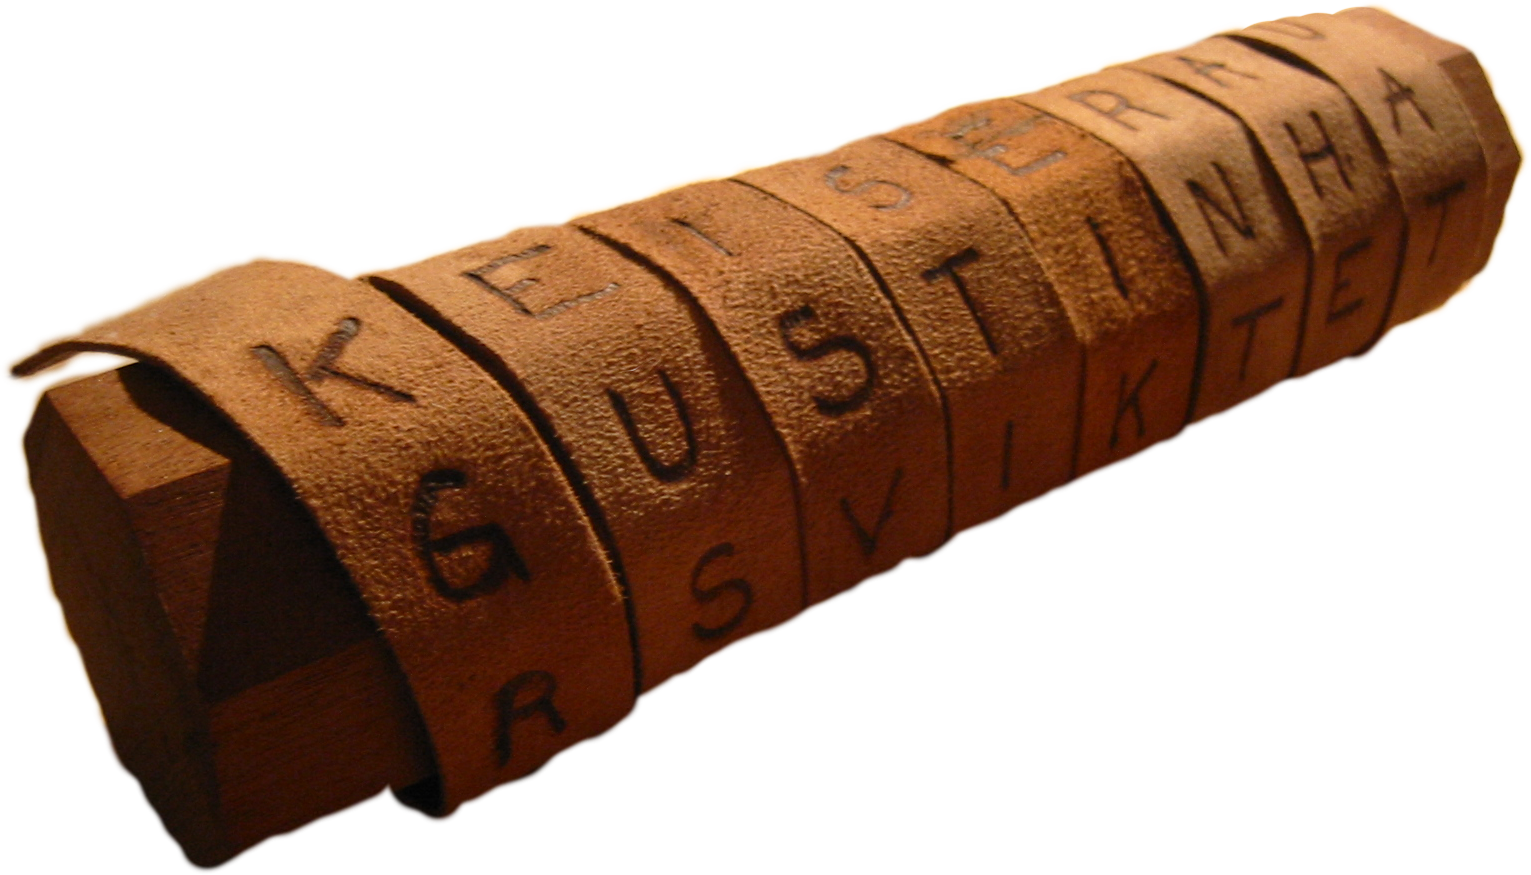
\includegraphics[width=\marginparwidth]{images/skytale}
\caption[]{Une scytale. Une bande de parchemin �tait enroul�e avant d'�crire le message, une lettre par tour. Une fois d�roul�, le parchemin �tait illisible � moins de poss�der une scytale du m�me diam�tre.}
 \label{figfr:scytale}
}

Les machines � chiffrement �lectrom�canique, telles que la fameuse machine Enigma, ont apport� une impressionnante augmentation des possibilit�s de chiffrement.
Lors de la seconde guerre mondiale, les efforts de cryptanalyse des chercheurs alli�s visant � casser les codes �lectrom�caniques men�rent au d�veloppement des premiers ordinateurs.
Cette perc�e mena finalement � l'utilisation d'algorithmes cryptographiques fond�s sur des probl�mes math�matiques complexes.
De plus, l'informatique permet le chiffrement de n'importe quel type de donn�es encod�es en s�quences de bits.
Le d�veloppement continu de l'informatique et des 'algorithmes de chiffrement publics ont rendu la s�curit� des communications accessibles aux petites entreprises et aux individus.
Aujourd'hui, les communications sont chiffr�es par d�faut, et les utilisateurs sont �duqu�s � pr�ter attention aux indicateurs de s�curit�~\cite{mozillasecurityblog2017communicating} tels que l'icone HTTPS repr�sentant un cadenas vert~\ref{figfr:firefox_warning}.
Cependant, un tiers de confiance est malgr�-tout souvent requis afin d'�tablir la communication.

Plusieurs d�finitions de la confiance ont �t� propos�es.
Inspir�s par McKnight et Chervany~\cite{mcknight1996meanings}, J�sang et Presti d�finissent la confiance comme: ``the extent to which one party is willing to depend on something or somebody in a given situation with a feeling of relative security, even though negative consequences are possible''~\cite{josang2004analysing}.
Dans le sens d'une action, nous dirions que la confiance est la d�cision par un agent intelligent de coop�rer face � une incertitude ou un risque au sujet du comportement (sa capacit� ou son intention) d'un autre agent.
La confiance est une heuristique bas�e sur l'historique des interactions, la r�putation donn�e par une communaut�, ou les recommandations transmises par d'autres sources de confiance.

La s�curit� des informations vise � prot�ger les informations �chang�es lors d'une communication, en s'assurant que certaines propri�t�s de s�curit� sont v�rifi�es:
\begin{itemize}
\item Le secret des �changes, la discr�tion (en: privacy),
\item La confidentialit� des messages �chang�s,
\item L'int�grit� du contenu,
\item La non-r�pudiation de la communication,
\item L'authentification de l'identit� des autres participants.
\end{itemize} 
                
Les syst�mes s�curis�s sont complexes � construire et peuvent �tre peu pratiques pour un usage quotidien.
Dans cette situation, la confiance peut �tre une fa�on plus confortable d'assurer la s�curit� des communications.

Le World Wide Web (le Web) est construit sur un mod�le client-serveur.
Sa s�curit� est bas�e sur une cha�ne de certificat ancr�e dans le User-Agent, g�n�ralement un navigateur Web.
Les sites Web sont authentifi�s par leurs certificats et les communications entre navigateurs et serveurs sont s�curis�es par des protocoles tels que TLS.
L'�mergence de nouvelles fonctionnalit�s du Web offre beaucoup plus de cas d'usage via l'utilisation d'une interface de programmation (API) JavaScript.
Ces nouvelles interactions sont souvent tripartites entre un utilisateur et deux autres serveurs: un Service Provider (SP) et un Relying Party (RP).
C'est par exemple le cas des sc�narios de d�l�gation d'authentification.
Dans ces situations, chaque partie ne peut pas monitorer les interactions entre les deux autres parties.
La s�curit� et la confiance de telles communications peuvent donc �tre plus dures � �valuer.
Chaque entit� doit alors baser ses d�cisions sur des crit�res subjectifs et sa propre �valuation du risque, donc prendre une d�cision de confiance.


\marginpar{
\captionsetup{type=figure}
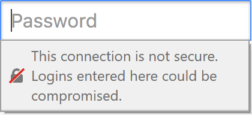
\includegraphics[width=\marginparwidth]{images/firefox_warning}\\\\
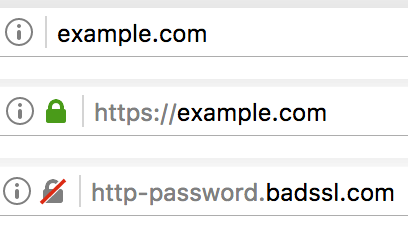
\includegraphics[width=\marginparwidth]{images/httpslevel}
\caption[]{Avertissements de s�curit� sur le navigateur Firefox.}
\label{figfr:firefox_warning}.
}

Les communications en temps r�el, sont un autre exemple de ces cas d'usage complexes impliquant plus qu'une simple relation client-serveur.
WebRTC est un ensemble d'API Web et de protocoles, sp�cifi�s par le W3C et l'IETF, permettant les appels audio, vid�o et le partage de donn�es en mode pair � pair.
Le d�ploiement de ce nouveau standard pourrait �tre une opportunit� d'ouverture des futurs services \gls{ott} [de l'acc�s internet].
Puisque WebRTC apporte de nouvelles fonctionnalit�s � l'�cosyst�me Web, sa s�curit� est un facteur critique de son succ�s.
Dans ce but, il est important que la sp�cification prenne en compte les probl�mes rencontr�s par les technologies pr�c�dentes.
C'est notamment vrai concernant la gestion d'identit�, en particulier compar�e � la qualit� de service.
Comme les exp�riences pr�c�dentes l'ont prouv�, un mod�le d'identit� fragile peut avoir un impact important et peut �tre particuli�rement dur � corriger une fois le syst�me d�ploy�. 


\section*{D�fis ouverts}
Notre intuition est que les utilisateurs de services de communication temps r�el devraient b�n�ficier de plus d'informations et de contr�le sur la s�curit� et le niveau de confiance de leurs sessions.
C'est notre objectif global.
Pour cela, nous devons construire un mod�le repr�sentant l'architecture de communication, les diff�rents canaux, protocoles et les acteurs impliqu�s.
Ce mod�le nous permettra de construire une m�trique caract�risant le risque d'utiliser un syst�me de communication, c'est-�-dire son niveau de confiance et de s�curit�.

Au vu de cet objectif, les questions suivantes sont ouvertes : 
Comment mod�liser une configuration de s�curit� d'une architecture de communication constitu�e de plusieurs canaux, protocoles et acteurs? 
Le m�me mod�le peut-il int�grer des informations de confiance et de s�curit� en une seule m�trique?
Quels param�tres de l'architecture de communication doivent �tre utilis�s pour construire cette m�trique?
Peut-on construire ce mod�le dynamiquement?

En supposant l'existence d'un mod�le de confiance et de s�curit� pour une architecture de communication, ce mod�le pourrait �tre utilis� pour agir sur le syst�me afin d'en augmenter  le niveau de confiance et de s�curit�.
Afin de donner ce genre de contr�le aux utilisateurs, nous devons aussi r�pondre aux questions suivantes:
Les utilisateurs peuvent-ils contr�ler le niveau de confiance et de s�curit� de leurs sessions de communication?
Est-il possible de faire confiance � une architecture de communication dans laquelle certains acteurs ne sont pas de confiance?
Les utilisateurs peuvent-ils choisir des acteurs de confiance pour l'�tablissement de leurs communications?

Afin de permettre aux utilisateurs de contr�ler la confiance et la s�curit� de leurs communications, la diversit� des configurations possibles doit �tre suffisamment �lev�e.
Cependant, les anciens syst�mes de communication t�l�phoniques ob�issent � des standards stricts.
Il peut y avoir plusieurs acteurs op�rant le r�seau, mais ils op�rent sous des configurations ferm�es et similaires.
Il y a aussi de nombreux services fournis \gls{ott}, mais ils op�rent en mode silo et en mode bo�te noire.
La diversit� de configuration de ces syst�mes est donc elle aussi basse.
Au contraire, WebRTC est une technologie Web disruptive.
Du fait de sa simplicit� , il est attendu que le nombre de services WebRTC explose dans un futur proche.
La version finale de WebRTC n'a pas encore �t� publi�e et certaines fonctionnalit�s restent � impl�menter dans les navigateurs.
C'est donc le bon moment pour �tudier l'architecture de s�curit� WebRTC.

\marginpar{
\captionsetup{type=figure}
\centering

\includegraphics[width=.6\marginparwidth]{images/webrtc}
\caption[]{Le logo de WebRTC.}
}

Pour ces raisons, nous souhaitons focaliser nos questions de recherche sur la sp�cification WebRTC.
Nous voulons comprendre � quel point les utilisateurs peuvent avoir confiance dans une session WebRTC, y compris si l'un des acteurs n'est pas de confiance.
Notre premi�re question de recherche est donc la suivante:

\begin{itemize}
\item \textbf{RQ1}: Quels sont les risques pour l'utilisateur d'une session WebRTC et quelle abstraction peut-on utiliser pour repr�senter ces risques aux utilisateurs?
\end{itemize}

Une fa�on de s'assurer qu'une session est s�curis�e est d'interagir avec des tiers de confiance, soit avant d'�tablir la session, soit lors de la session pour en augmenter le niveau de confiance et de s�curit�.
Cela pose les questions suivantes:

\begin{itemize}
\item \textbf{RQ2}: Peut-on agir sur une session WebRTC afin d'en augmenter le niveau de confiance et de s�curit�?
\item \textbf{RQ3}: Peut-on laisser les utilisateurs choisir des acteurs de confiance pour l'�tablissement de la communication?
\end{itemize}

\section*{Contributions}
Dans cette th�se, je propose trois contributions principales:

\subsection*{Discr�tion li�e � l'architecture d'identit� de WebRTC}
Dans notre premi�re contribution, nous �tudions l'architecture d'identit� WebRTC et plus particuli�rement son int�gration aux algorithmes de d�l�gation d'authentification existants.
Cette int�gration n'a pas encore �t� �tudi�e jusqu'� pr�sent.
Dans cette perspective, nous impl�mentons les composants de l'architecture d'identit� WebRTC ce qui nous permet de montrer que cette architecture n'est pas particuli�rement adapt�e � une int�gration aux protocoles de d�l�gation d'authentification existants tels qu'OpenID Connect.
Pour r�pondre � RQ1, nous montrons ensuite comment la position centrale des fournisseurs d'identit� dans l'�cosyst�me du Web est renforc�e par leur int�gration � l'�tablissement de session WebRTC, posant ainsi un risque suppl�mentaire contre la discr�tion des utilisateurs.
Dans l'�cosyst�me Web, la norme est l'architecture des services en silo dont les utilisateurs sont captifs.
C'est en particulier le cas des syst�mes de d�l�gation d'authentification, pour lesquels la plupart du temps, il n'est pas possible de choisir son fournisseur d'identit�.
Afin de r�pondre � RQ3, nous r�alisons une �tude afin de d�terminer pour quelles raisons les utilisateurs ne peuvent pas choisir leur fournisseur d'identit� sur Web.
Notre �tude montre que bien que ce choix soit possible en th�orie, l'absence d'impl�mentation de certains standards par les sites webs et les fournisseurs d'identit� emp�che ce choix en pratique.

\marginpar{
\captionsetup{type=figure}
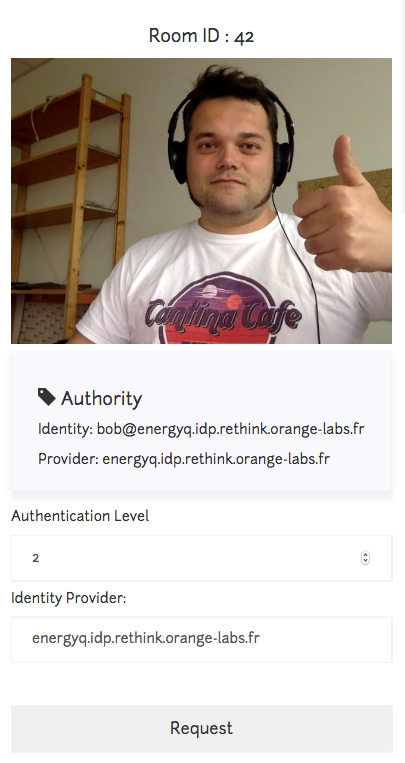
\includegraphics[width=.9\marginparwidth]{images/acor_negotiation}
\caption[]{Notre interface de n�gotiation d'identit� sur un service WebRTC.\\\\\\ }
\label{figfr:acor}
}

\subsection*{Controller les param�tres d'identit� de WebRTC}
Dans notre seconde contribution, nous cherchons � donner plus de contr�le � l'utilisateur.
Pour ce faire et en r�ponse � RQ2, nous proposons une extension de la sp�cification WebRTC afin de permettre la n�gociation des param�tres d'identit�.
Un prototype d'impl�mentation est propos� afin de valider notre proposition (voir Figure~\ref{figfr:acor}).
Cette impl�mentation r�v�le certaines limites dues � l'API d'identit� WebRTC emp�chant notamment d'obtenir un retour sur le niveau d'authentification de l'autre utilisateur ainsi que l'impossibilit� de changer de fournisseur d'identit� en cours de session.
Nous proposons ensuite une API Web permettant aux utilisateurs de choisir leur fournisseur d'identit� lors d'une authentification sur un site tiers via une interface de s�lection d'identit� contr�l�e par le navigateur.
R�pondant � RQ3, notre API repose sur une r�utilisation de l'architecture d'identit� WebRTC dans un sc�nario client-serveur.
Nous pr�sentons une impl�mentation de notre solution, bas�e sur une extension du navigateur Firefox, afin d'en d�montrer l'utilisabilit� (voir Figure~\ref{figfr:webconnect}).
Nos r�sultats montrent qu'� long terme, l'adoption de cette API pourrait r�duire la charge d'impl�mentation pour les d�veloppeurs de sites Web et permettre aux utilisateurs de pr�server leur discr�tion en choisissant des fournisseurs d'identit� de confiance.


\marginpar{
\captionsetup{type=figure}
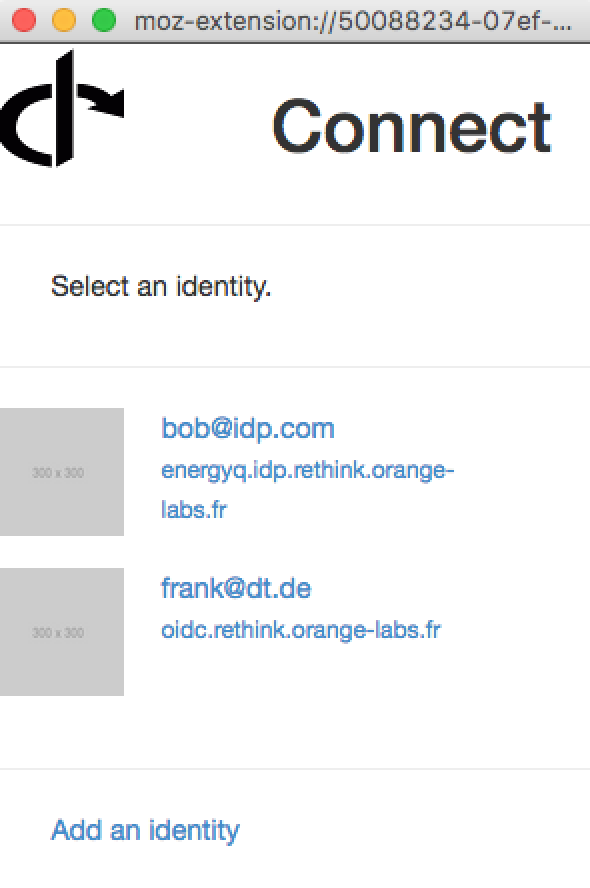
\includegraphics[width=.9\marginparwidth]{images/WebConnect}
\caption[]{L'interface de s�lection d'identit� de WebConnect.}
\label{figfr:webconnect}
}


\subsection*{Un mod�le de confiance et de s�curit� pour WebRTC}
Enfin dans notre troisi�me contribution, nous r�pondons � RQ1 en proposant un mod�le de confiance et de s�curit� d'une session WebRTC.
Ce mod�le int�gre en une seule m�trique les param�tres de s�curit� utilis�s lors de l'�tablissement de la session, les param�tres d'encryption des flux m�dia, et les param�tres de confiance de l'utilisateur dans les acteurs de la session WebRTC.
L'objectif de notre mod�le est dans un premier temps de permettre aux utilisateurs non-experts de mieux comprendre la s�curit� de leurs sessions WebRTC.
Afin de valider notre approche, nous r�alisons une exp�rimentation pr�liminaire �valuant la compr�hension de notre mod�le par des utilisateurs non-experts en s�curit�. 

\section*{Publications}
Mes travaux ont �t� le sujet de plusieurs publications et contributions, en voici la liste:

\subsection*{Publications Scientifiques}
\begin{description}
\item \cite{corre_webrtc_2017} \fullcite{corre_webrtc_2017}
\item \cite{corre_whyusers_2017} \fullcite{corre_whyusers_2017}
\item \cite{javed_cross-domain_2017} \fullcite{javed_cross-domain_2017}
\end{description}

\subsection*{Internet Drafts}
\begin{description}
\item \cite{I-D.copeland-rtcweb-p2p-idp-auth} \fullcite{I-D.copeland-rtcweb-p2p-idp-auth}
\end{description}

\paragraph{A note on RFC} Requests For Comments are documents published by the IETF and describing technical aspects of the internet.
RFC are first proposed as \textit{draft} with an expiration date of 6 months, which can be extended by submitting new version of the draft.
If an interest emerge, a working group may form.
This working group will develop the draft further until a request to publish it as a RFC is submitted.
Not all RFCs are however submitted on the standard track.
Their status may alternatively be \textit{informational}, \textit{experimental}, \textit{best current practice}, \textit{historic}, or \textit{unknown}.

\subsection*{Brevets}
\begin{description}
\item \cite{corre_authent} \fullcite{corre_authent}
\end{description}

\subsection*{Rapports Techniques}
\begin{description}
\item \cite{copeland_framework_2015} \fullcite{copeland_framework_2015}

\item \cite{crom_management_2015} \fullcite{crom_management_2015}

\item \cite{crom_implementation_2016} \fullcite{crom_implementation_2016}

\item \cite{crom_implementation_2017} \fullcite{crom_implementation_2017}

\end{description}


Cette th�se pr�sente le r�sultat de notre travail de recherche conduit lors des trois derni�res ann�es. Il est le r�sultat d'une collaboration entre l'�quipe Identity and Trust Architecture d'Orange Labs et l'�quipe DiverSE de l'INRIA.
Nous avons aussi contribu� au projet H2020 reThink, en particulier � l'architecture d'identit� et de s�curit�.

\clearpage

\newgeometry{
            left=2.2cm,
            right=2.2cm,
            top=2.2cm,
            bottom=3.5cm,
            ignoremp}
\renewpagestyle{scrheadings}{
  {\makebox[2em][r]{\thepage}\quad\rule{1pt}{100pt}\quad\leftmark}%
  {\hfill\rightmark\quad\rule{1pt}{100pt}\quad\makebox[2em][l]{\thepage}}%
  {}
}{
  {}%
  {}%
  {}
}
\renewpagestyle{plain.scrheadings}{
  {}%
  {}%
  {}
}{
  {\thepage}%
  {\hfill\thepage}%
  {}
}
\chapter*{Abstract}
\addcontentsline{toc}{chapter}{Abstract}
\thispagestyle{empty}
\glsresetall
Nowadays, communications transiting through the Internet are encrypted by default, often end-to-end.
Secure communication is a commodity accessible to everyone rather than restricted to powerful organisations.
Users are being educated to the security risks faced on the internet and to pay attention to security indications.
But this does not solve every security issues: a trusted third party is still required in order to setup the communication.
Security on the Web is based on a certificate chain anchored into the web browser.
The emerging web functionalities offer a lot more possible use-cases than the usual client-server communication.
Real-time media and data communication is one of these complex use-cases which involves peer-to-peer and full-duplex client-server communications.
On one hand legacy inter-operable communication systems suffer from issues regarding the trustworthiness of their incoming call.
On the other hand over-the-top communication networks are all set in a silo model: users are de-facto captive of these services.

WebRTC is a set of standard web API and protocols, which supports peer-to-peer audio-video calling and data sharing.
It is envisioned, given the simplicity to deploy a WebRTC services, that the number of WebRTC enabled websites could skyrocket in the near future.
To succeed, WebRTC should improve from the issues encountered by previous technologies.
A weak identity model may have an important impact later on and is particularly hard to fix once the system is deployed.
Considering the various use cases and the possible number of services and other actors, the complexity of a communication setup could be really difficult to assess by non-expert users.

Our intuition is that users should be given more informations and control on the security and trust level of their communications.
We want to build a model that could represent the communication setup, the different channels, protocols, and actors in operations.
This model would allow us to act on the system in order to raise the trust and security level.
At the moment, WebRTC's final version of the specification has not yet been published, and some functionalities are yet to be implemented in Web Browsers.
It may be the right time to challenge its security architecture by addressing the following research questions:

\begin{itemize}
\item \textbf{RQ1}: What are the risks for the user of a WebRTC session and which abstractions can we use to show these risks to the user?
\item \textbf{RQ2}: Can we act on a WebRTC session to raise the trust and security level? 
\item \textbf{RQ3}: Can users choose actors they trust to participate in the communication setup?
\end{itemize}

In this thesis, we propose three main contributions:

In our first contribution we study the WebRTC identity architecture and more particularly its integration with existing authentication delegation protocols.
This integration has not been studied yet. 
To fill this gap, we implement components of the WebRTC identity architecture and comment on the issues encountered in the process.
In order to answer RQ1, we then study this specification from a privacy perspective an identify new privacy considerations related to the central position of identity provider.
In the Web, the norm is the silo architecture of which users are captive.
This is even more true of authentication delegation systems where most of the time it is not possible to freely choose an identity provider.
In order to answer RQ3, we conduct a survey on the top 500 websites according to Alexa.com to identify the reasons why can't users choose their identity provider.
Our results show that while the choice of an identity provider is possible in theory, the lack of implementation of existing standards by websites and identity providers prevent users to make this choice.

In our second contribution, we aim at giving more control to users.
To this end and in order to answer RQ2, we extend the WebRTC specification to allow identity parameters negotiation.
We present a prototype implementation of our proposition to validate it.
It reveals some limits due to the WebRTC API, in particular preventing to get feedback on the other peer's authentication strength.
We then propose a web API allowing users to choose their identity provider in order to authenticate on a third-party website, answering RQ2.
Our API reuse components of the WebRTC identity architecture in a client-server authentication scenario. 
Again, we validate our proposition by presenting a prototype implementation of our API based on a Firefox extension.

Finally, in our third contribution, we look back on RQ1 and propose a trust and security model of a WebRTC session.
Our proposed model integrates in a single metric the security parameters used in the session establishment, the encryption parameters for the media streams, and trust in actors of the communication setup as defined by the user.
Our model objective is to help non-expert users to better understand the security of their WebRTC session.
To validate our approach, we conduct a preliminary study on the comprehension of our model by non-expert users.
This study is based on a web survey offering users to interact with a dynamic implementation of our model.
\cleardoublepage

\tableofcontents
\clearpage

\restoregeometry
\renewpagestyle{scrheadings}{
  {\hspace{-\marginparwidth}\hspace{-\marginparsep}\makebox[\overflowingheadlen][l]{\makebox[2em][r]{\thepage}\quad\rule{1pt}{100pt}\quad{}\leftmark}}%
  {\makebox[\overflowingheadlen][r]{\rightmark\quad\rule{1pt}{100pt}\quad\makebox[2em][l]{\thepage}}}%
  {}
}{
  {}%
  {}%
  {}
}
\renewpagestyle{plain.scrheadings}{
  {}%
  {}%
  {}
}{
  {\thepage}%
  {\makebox[\overflowingheadlen][r]{\thepage}}%
  {}
}


%%%%%%%%%%
% MAIN MATTER
\mainmatter
%%%%%%%%%%
\chapter*{Introduction}
\label{introduction}
\addcontentsline{toc}{chapter}{Introduction}
\glsresetall
\section*{Context}
\label{introduction.context}

Communications, deriving from the Latin \textit{communicatio}~\cite{communicatio}, is defined by the Oxford dictionary as ``the imparting or exchanging of information'' and ``the means of sending or receiving information, such as telephone lines or computers''~\cite{communication}.
In case of uncertainty and risk, such exchange is made possible if a trust relation can be established between the senders and receivers.
This trust relation must also cover the channels used to communicate.
Written communications were developed through several revolutions: from immobile chiselled pictograms to electronic signals instantly replicated and transmitted.
While these revolutions made communications more and more pervasive, the fundamental issue of trust remains.
Politicians and military commanders may always have had a need for secure communications, and for long the concept of secure communication was equivalent to the confidentiality of a message. 
Steganography, the fact of hiding a message in plain sight, was the earliest technique to secure a written communication. 
It can be achieved by using an invisible ink or by inserting a message inside another document, for instance, using bits of a numerical image to encode a secret text.
Cryptography, on the other hand, is a technique transforming a secret message, called a plaintext, into an encrypted cyphertext in order to hide its meaning.
The first known evidence of cryptography is an engraved pottery from 1900bc.
The Spartan scytale, shown in Figure \ref{fig:scytale}, was the first known institutional military cypher, reported as being used in 404~B.C.~\cite{singh2000code}.

\marginpar{
\captionsetup{type=figure}
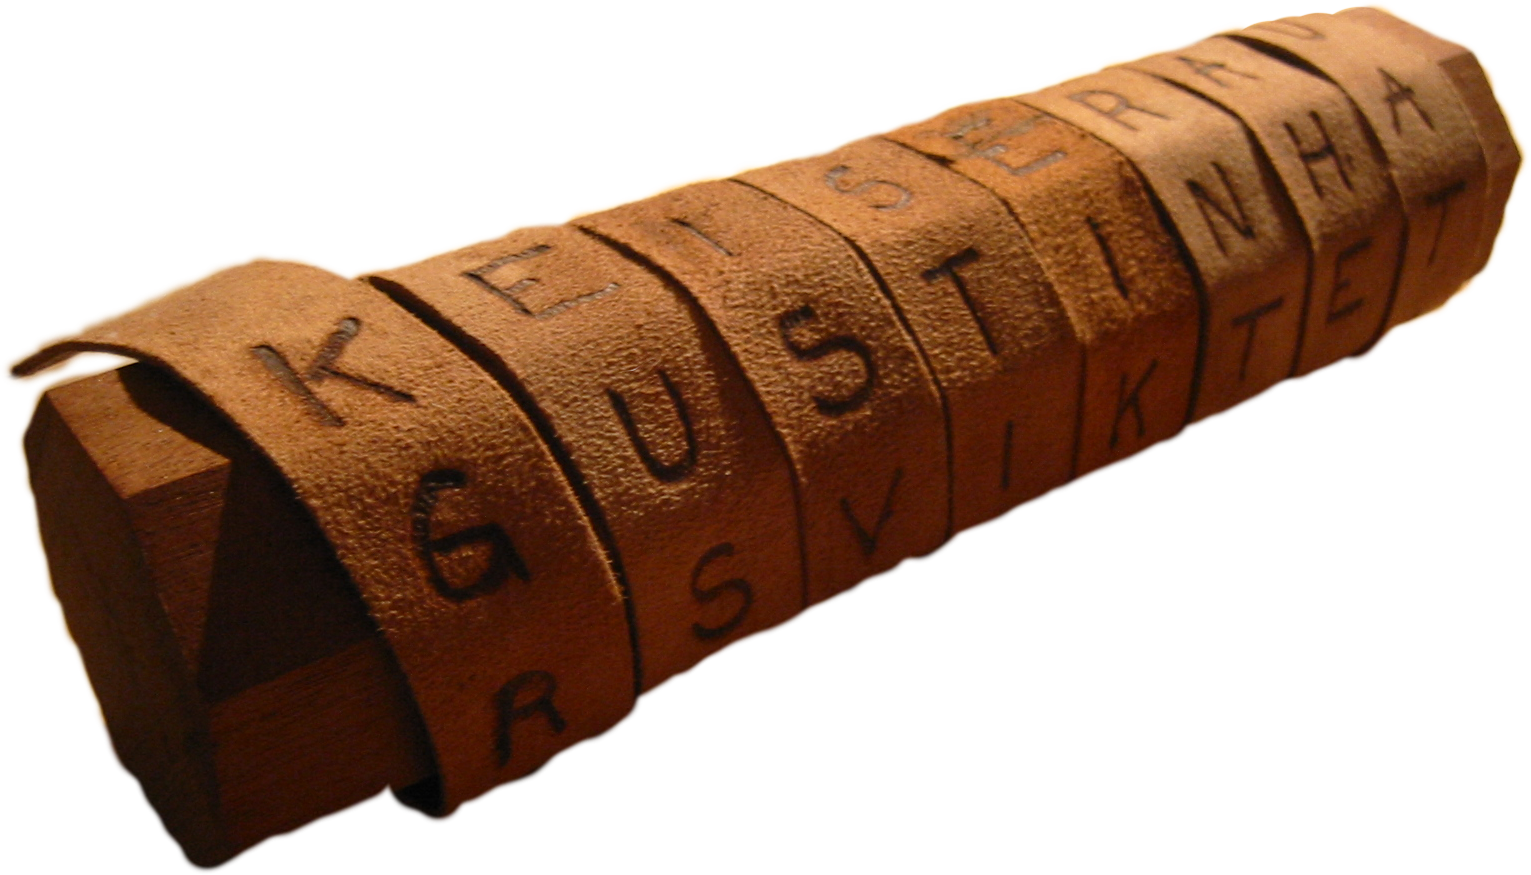
\includegraphics[width=\marginparwidth]{images/skytale}
\caption[A Scytale]{A band of parchment was first wrapped around the scytale, then the message was written one letter per convolution. Once unfolded, the message would be unreadable except for the receiver which would have another scytale of the same diameter. }
\label{fig:scytale}
}

Caesar's cypher may be one of the simplest cryptographic technique.
In this technique, letters are replaced by another letter at a given distance in the alphabet.
Julius Caesar was reported as using this cypher with a shift of three letter to write secret messages to his generals.
Knowing the shift value, \ie the secret key, a recipient of an encrypted message could reverse the shift to uncover the plaintext message.
Alberti invented around 1467 a polyalphabetic substitution cypher where the key is modified at random through the text.
Though later works derive from Alberti's invention, such cryptography technique was already known by the 8th century's mathematician Al-Kindi.
Substitution cyphers are vulnerable to letter frequency attack.
Indeed, a cryptanalyst can guess the key of a simple substitution cypher by comparing the letter frequencies of the cyphertext to the letter frequencies of another plaintext known to be written in the same language.
Polyalphabetical substitutions try to alter the frequency of letters by continuously changing the substitution alphabet.
These are however still vulnerable to more complex frequency analysis.
The development of substitution cyphers was thus a race between cryptographers inventing new keying mechanisms and cryptanalysts.

Rotor machines, such as the famous Enigma machine, brought a large increase in the number of possible substitutions. 
Cryptanalysis efforts by allied researchers during the second world war resulted in the development of the first programmable computer.
This breakthrough also allowed the use of much more complex cyphers based on complex mathematical problems.
Furthermore, computers allow the encryption of any kind of data encoded as a sequence of bits.
The development of computer and public cryptographic algorithms made security accessible to small companies and individuals. 
Everyday communications are now encrypted by default, and users are being educated to pay attention to security indications~\cite{mozillasecurityblog2017communicating} such as the one presented in Figure~\ref{fig:firefox_warning}.
This, however, does not solve every issue: a trusted third party is still often required to set up the communication.

\marginpar{
\captionsetup{type=figure}
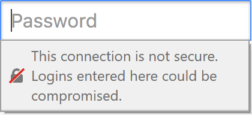
\includegraphics[width=\marginparwidth]{images/firefox_warning}\\\\
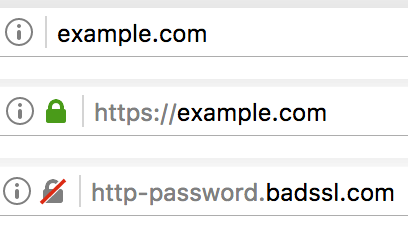
\includegraphics[width=\marginparwidth]{images/httpslevel}
\caption[Browser Security Indications]{By displaying warning on insecure HTTP webpage, the Firefox web browser is educating its users to the faced risk, and at the same time pushing web developers to implement security for HTTP.}
\label{fig:firefox_warning}
}

%% TRUST DEFINITION

Several definitions of trust have been proposed.
Inspired by McKnight and Chervany~\cite{mcknight1996meanings}, J{\o}sang and Presti define trust as: ``the extent to which one party is willing to depend on something or somebody in a given situation with a feeling of relative security, even though negative consequences are possible''~\cite{josang2004analysing}.
In the sense of an action, we would say that trust is the decision of intelligent agents to cooperate in the face of risk and uncertainty about the behaviour (capability or intention) of other agents.
This heuristic is often based on prior interaction history, reputation from a community or recommendations from other trusted sources.
 
%% SECURITY DEFINITION
Information security, on the other hand, aims at protecting information exchanged during a communication, by ensuring that certain security properties are met:
\begin{itemize}
\item The secrecy of the exchange, \ie the \textit{privacy}.
\item The \textit{confidentiality} of the exchanged message.
\item The \textit{integrity} of the content.
\item The \textit{non-repudiation} of the communication.
\item The \textit{authentication} of the other peer's identity.
\end{itemize}

Fully secure systems are difficult to build and may be impractical for everyday usage. 
In this situation, trust may be a more relaxed way of ensuring the security of the communication.

The World Wide Web (in short: the Web) is built on a client-server model.
Its security is based on a certificate chain anchored into the \gls{ua}, usually a web browser, acting as the \gls{tcb}.
Websites are authenticated by their certificates and communications between the \gls{ua} and the server are secured by protocols such as \gls{tls}. 
The emerging web functionalities offer a lot more possible use-cases through JavaScript web \gls{api} and \gls{http}~\cite{RFC2616} based protocols.
These new relations are often tripartite between a user and two other servers, a service provider and a \gls{rp}.
This is, for instance, the case in authentication delegation scenarios.
In these tripartite situations, each party cannot fully monitor interactions between the others parties.
The security and trustworthiness of such communication may be more difficult to assess.
As a result, it is up to each entity to take a decision based on subjective criteria and its own evaluation of the faced risk, \ie to take a trust decision.

Real-time media and data communication is another complex use-case involving more than a single client-server relation.
On one hand, legacy inter-operable communication systems, operated by telephony companies and Internet service providers (often referred as Telco) have been cluttered by issue regarding the trustworthiness of their incoming call.
These legacy services suffer from a weak trust and identity model which is subject to abuse.
The openness of trust-circle networks and the availability of computation power allow malicious actors to launch thousands of robocalls at once\footnote{In 2014, the United States' Federal Trade Commission has received over 22 million complaints about illegal and unwanted phone calls~\cite{tu2016sok}.
Even though the practice of phone spam is illegal in the European Union without an opt-in from the recipient, in France 1,6 million voice and SMS spams were reported in 2016 to the 33700, the national spam reporting number~\cite{33700}.}.
This factor could be one of the reasons behind the drop of value in telephony services~\cite{arcep_observatoire}, a major asset of Telco, benefiting to \gls{ott}\footnote{\gls{ott} services are provided on top of existing internet service providers networks} services.
On the other hand, \gls{ott} are rapidly gaining market share over Telco but are all set in silo model.
The silo model implies that while these services benefit from a controlled trust model, they cannot communicate with each other and are the theatre of an intensive battle to become, or stay, the hegemonic service\footnote{Chocking examples of this competition were the buyout of Whatsapp and its 450 millions users in 2014 by Facebook for \$16 billions~\cite{goel_facebook}, and the buyout of Skype and its 663 millions users by Microsoft in 2011~\cite{rosoff_microsoft}. In particular, the Skype buyout was conducted after rumours of interest from Cisco, Google, and Facebook, \ie Microsoft's competitors.}.
As it is difficult to change network without losing the ability to reach their contacts, users are de-facto captive of these services.

WebRTC is a set of web \gls{api} and protocols, specified by the \gls{w3c} and the \gls{ietf}, which supports \gls{p2p} audio-video calling and data sharing.
As WebRTC brings useful new functionalities to the web ecosystem, its deployment could be an opportunity to open the future \gls{ott} services.
For the WebRTC specification to succeed, it should learn from the issues encountered by previous technologies.
As past experiences have proved~\cite{RFC5039}, a weak identity model may have an important impact later on and is particularly hard to fix once the system is deployed.

\section*{A Motivating Scenario}
\label{introduction.scenario}
%Currently the main WebRTC use case is to easily integrate real-time communication into a webpage.
In a conference call, several users connect to a single room to organise a meeting.
Users share their audio and video, they may also share some documents or their screen~\cite{w3c:screencapture}.
%WebRTC is particularly fitting to this use case due to the possibility to open media and data channels.
%Technically, sessions between users may be organised in a mesh topology, but more realistically an efficient architecture would use a Multipoint Control Unit. 
Several communication services are already offering this kind of service, some using WebRTC. 
However, a common issue appears when participants connect from different company, for instance during a collaborative project.
While the service is often integrated with one company's \gls{idp}, participants from other companies may not authenticate with it and may have to fallback to a declarative or self-asserted identity.
Because the subject of their conversation is sensible, participants want to ensure that no one is maliciously listening, including the communication service itself which may come from a third party company.
Currently, implementation decisions made by the \gls{cs} website drastically limit the user's choice.
And at the same time communication services are missing the capability to interface with any \gls{idp}.

Going further, supposing every participant authenticated to each other, one of them may want to raise the security level of the session.
Each participant would then be required to authenticate with a higher strength, and the session security would be renegotiated with stronger parameters.
For this to be possible, it is required to have a model of the trust and security level of the session and a mechanism to negotiate it.
In the long-term, the future telephony will move to a fully IP-based network, interconnected with the Web.
In this scenario, inter-operability, \ie the ability for a user of one \gls{cs} to call a user from another \gls{cs}, could be imposed by regulations.
Some projects are already writing work in progress inter-operable \gls{cs} architectures~\cite{toutain2015webco,matrix,rethink}.
Evaluating the security of a call session is necessary for users to make an informed trust decision on whether or not to accept or pass a call.
However, in these inter-operable architectures, the communication stack is drastically more complex than the usual client-server model.

\section*{Open Challenges}
\label{introduction.challenges}
Our intuition is that users should be given more information and control over the security and trust level of their communications.
This is our global objective.
For this to be possible, we need to build a model that could represent the communication setup, the different channels, protocols, and the actors in operation.
This model would allow us to forge a single metric characterising the risk of using the communication system, \ie the trust and security level.
It would also be a useful tool to model an instance of a communication setup specification and discuss it with expert.

To inform the user of the security of its communication session, it is necessary to answer the following questions:
\begin{itemize}
\item How to model the security of a communication setup made with several distinct channels, protocols, and actors?
\item Can the same model integrate trust and security information into a single meaningful metric?
\item Which parameters of the communication setup can be used to forge this metric?
\item Can we build this model at runtime?
\end{itemize}

Supposing we dispose of a trust and security model for the communication setup, we could leverage this model to raise the trust and security level of the session.
This process could either be manually or automatically controlled by the user.
To give this kind of control to the users, we would also have to answer the following questions:
\begin{itemize}
\item Can users control and eventually raise the trust and security level of their communication sessions?
\item Is it possible to trust a communication setup in which some of the actors are not trusted?
\item Can users choose trusted actors to participate in their communication setup?
\end{itemize}

As we mentionned, legacy communication services obey strict standards allowing interoperability between actors.
%There may be several actors on the network, but they operate under the same configurations.
There are also multiple \gls{ott} communication services, but since they are set in silo and often operate closed-source softwares, we consider them as blackboxes.
WebRTC, however, is a disruptive technology for web real-time communications.
It is envisioned, given the simplicity to deploy a WebRTC service, that the number of WebRTC enabled websites could skyrocket in the near future.
Considering the proposed use cases, the number of WebRTC services, and the other actors: the complexity of communication setup, from a trust and security perspective, could be difficult to assess for non-expert users.
At the moment, WebRTC's final version of the specification has not yet been published, and some functionalities are yet to be implemented in web Browsers\footnote{The state of WebRTC implementations on web browsers can be followed on Mozilla's developer website: \url{https://developer.mozilla.org/en-US/docs/Web/API/RTCPeerConnection}.}.
It may be the right time to challenge its security architecture.

For these reasons, we want to address our research questions with respect to the WebRTC specifications.
We want to understand to which extent users could trust a WebRTC session, even if some parties are untrusted.
Our first research question is thus the following:

\begin{itemize}
\item \textbf{RQ1}: What are the risks for the user of a WebRTC session and which abstractions can we use to show these risks to the user?
\end{itemize}

One way to ensure that the session is secured is to interact with trusted parties, either before the session is established, or during the session to raise the trust level.
This opens the two following questions:
\begin{itemize}
\item \textbf{RQ2}: Can we act on a WebRTC session to raise the trust and security level? 
\item \textbf{RQ3}: Can we let users chose actors they trust to participate in the communication setup?
\end{itemize}

\section*{Contributions}
\label{introduction.contributions}
In this thesis, I propose three main contributions:

In our first contribution, we study the WebRTC identity architecture and more particularly its integration with existing authentication delegation protocols.
This integration has not been studied yet. 
To fill this gap, we implement components of the WebRTC identity architecture and comment on the issues encountered in the process.
In order to answer RQ1, we then study this specification from a privacy perspective and identify new privacy considerations related to the central position of \gls{idp}.
In the Web, the norm is the siloed architecture of which users are captive.
That is all the more the case for authentication delegation systems where most of the time it is not possible to freely choose an \gls{idp}.
In order to answer RQ3, we conduct a survey of the top 500 websites according to Alexa\footnote{\url{https://alexa.com}} to identify the reasons why users cannot choose their \gls{idp}.

In our second contribution, we aim at giving more control to users.
To this end and in order to answer RQ2, we extend the WebRTC specification to allow identity parameters negotiation.
We present a prototype implementation of our proposition to validate our proposition.
We then propose a web \gls{api} allowing users to choose their \gls{idp} in order to authenticate on a third-party website.
Our \gls{api} reuse components of the WebRTC identity architecture in a client-server authentication scenario. 
Again, we validate our proposition by presenting a prototype implementation of our \gls{api} based on a Firefox extension.

Finally, in our third contribution, we look back on RQ1 and propose a trust and security model of a WebRTC session.
Our proposed model integrates into a unique metric the security parameters used in the session establishment, the encryption parameters for the media streams, and trust in actors of the communication setup as defined by the user.
Our model's objective is to help non-expert users to better understand the security of their WebRTC session.
To validate our approach, we conduct a preliminary study on the comprehension of our model by non-expert users.
This study is based on a web survey offering users to interact with a dynamic implementation of our model.

Figure~\ref{contrib} represents how our contributions articulate and how they relate to our research questions.
In our first contribution we study the WebRTC identity architecture.
We then experiment on how to control this identity architecture to increase trust and security.
Finally and based on our knowledge, we close the loop and propose a model of the trust and security of the WebRTC security architecture.
 
\begin{figure}[H]
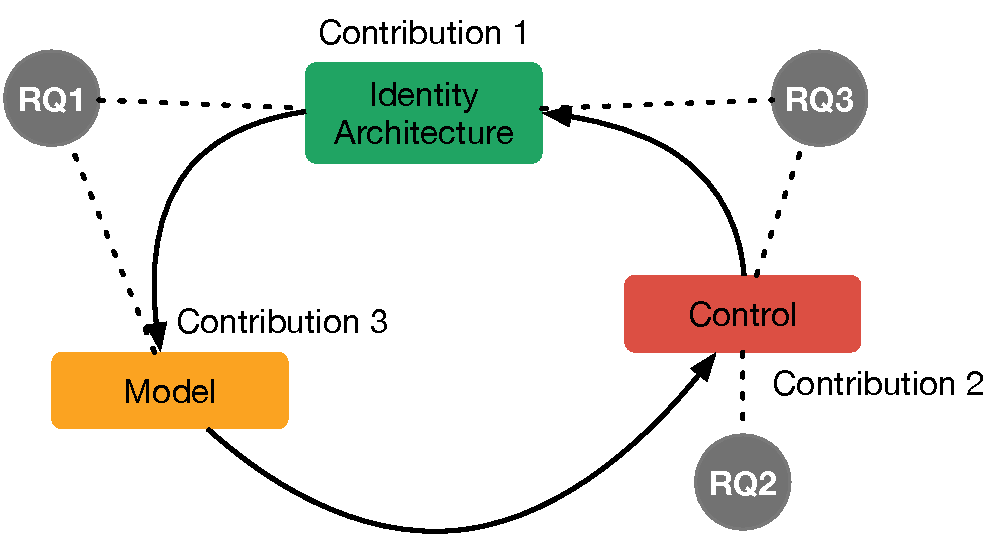
\includegraphics[scale=.5]{images/controlloop}
\caption{Overview of our Contributions}
\label{contrib}
\end{figure}


%
%\begin{figure}[tbp]
%\begin{center}
%    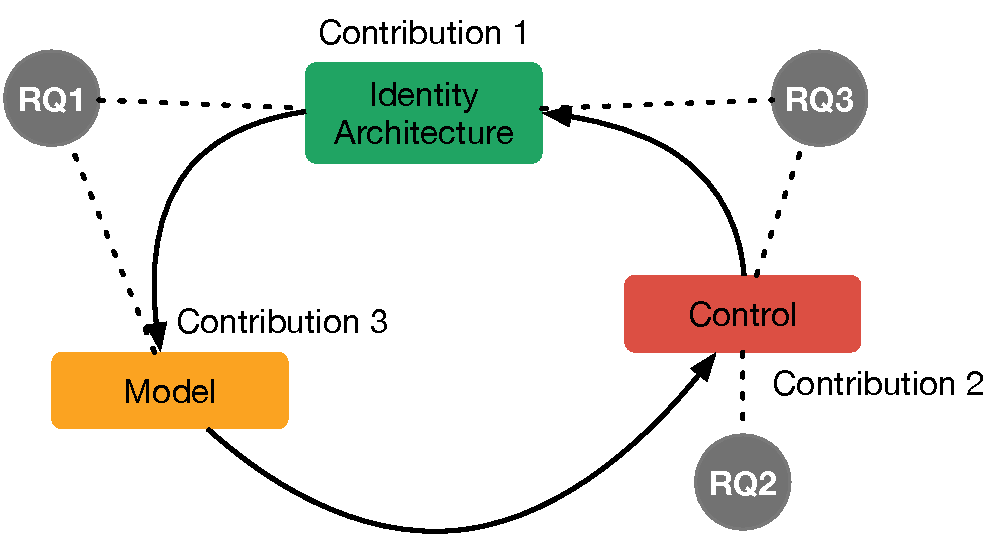
\includegraphics[width=\linewidth]{images/controlloop}
%\end{center}
%    \begin{tikzpicture}
%    \node(rq1)[rectangle, minimum width=0.6cm, minimum height=0.4cm, fill=matgreen] at (-1,0) {};
%    \node[] at (-.1,0) {\footnotesize RQ1};
%    \node(rq2)[rectangle, minimum width=0.6cm, minimum height=0.4cm, fill=matred] at (-1,-.5) {};
%    \node[] at (-.1,-.5) {\footnotesize RQ2};
%    \node(rq3)[rectangle, minimum width=0.6cm, minimum height=0.4cm, fill=matblue] at (-1,-1) {};
%    \node[] at (-.1,-1) {\footnotesize RQ3};
%    \node[] at (8,0) {};
%    \end{tikzpicture}
%\caption{Trust and security level control loop and related research questions.}
%\label{fig_controlloop}
%\end{figure}
%
%A way to represent our research questions and contributions is a control loop for the trust and security level of a WebRTC session, as present in Figure~\ref{fig_controlloop}.
%The goal of RQ1 is to build a sensor and a model, together capable of measuring the trust and security level of the session.
%In RQ2 we search to act on the session to raise the security level.
%Finally, in RQ3 we try to determine if and how users could choose trusted actors, in order to raise the trust level of the communication setup.
%

\section*{Organisation}
\label{introduction.organisation}
The document is organised in three main parts.
In the first part, we expose the context of our research.
In Chapter~\ref{security}, we detail the technical specifications used in our work such as OAuth~2 and WebRTC.
We then present the state of the art to which our work contributes in Chapter~\ref{sota}.
In the second part of this thesis, we present our contributions.
In Chapter~\ref{webrtcprivacy} we study WebRTC privacy issues based on actual implementations of the WebRTC identity architecture.
In Chapter~\ref{identitynegotiation} we propose to give users more control over their WebRTC identity parameters.
Chapter~\ref{webrtcmodel} presents a trust and security model of a WebRTC session intended to help advanced users in understanding the security of their WebRTC session.
Finally, the third part of this thesis proposes a summary of our contributions in Chapter~\ref{conclusion} and discusses our perspectives in Chapter~\ref{perspectives}.

\subsection*{Part \ref{context}:  Context}
\paragraph{Chapter \ref{security}} \textit{WebRTC Trust and Security Architecture} is an introduction to the techniques, algorithms, and protocols securing WebRTC and forming the context of our thesis.
In this chapter, we introduce the WebRTC architecture and specifications, present an overview of the concepts accomplishing practical security on the Web, and focus on the protocols used to secure a WebRTC communication.
We also introduce the concept of trust and we explain privacy in the context of the Web and in particular the privacy consideration of the WebRTC specification.
Finally, we present some signalling architecture that could be deployed by WebRTC services.

\paragraph{Chapter \ref{sota}} \textit{State of the Art} presents the state of the art on \gls{voip} security research.
We review the results of a comprehensive survey of 245 articles on \gls{voip} security and published in 2012.
As the first draft of the WebRTC specification was published the same year, this survey is a solid starting point to study the field of WebRTC security.
We then present our own survey of \gls{voip} and WebRTC security research collecting papers published between 2012 and 2017.
Based on our findings, we review collected papers dealing specifically with WebRTC.


\subsection*{Part \ref{contributions}: Contributions}
\paragraph{Chapter \ref{webrtcprivacy}} \textit{Privacy Implications of the WebRTC Identity Architecture} studies the WebRTC identity architecture from a privacy point-of-view.
The specification lacks support and, to the best of our knowledge, there is no public implementation.
We first describe our implementation of the WebRTC identity architecture and its integration with existing authentication delegation protocols.
We then comment on encountered issues and detail additional privacy considerations.
Finally, we report on our study on why users cannot choose their \gls{idp} on the Web. 


\paragraph{Chapter \ref{identitynegotiation}} \textit{Controlling the WebRTC Identity Parameters} proposes to give users more control over WebRTC identity parameters.
Firstly, we define a \gls{sdp} extension to negotiate the other peer's \gls{idp} and authentication strength during the call setup and present our implementation.
Secondly, this chapter presents WebConnect, a prototype for an Identity Metasystem \gls{api} based on the WebRTC identity specification which allows users to preserve their privacy by selecting trusted \gls{idp}.
The WebRTC identity specification offers some interesting concepts limited to the scope of user-to-user authentication, WebConnect extends them to the use case of user-to-server authentication.


\paragraph{Chapter \ref{webrtcmodel}} \textit{WebRTC Trust and Security Model} presents a trust and security model intended to help advanced users in understanding the security of their WebRTC session.
We first present our methodology to build our model and then details our actual WebRTC trust and security model.
The model evaluates security with regards to the risk presented on the confidentiality and integrity of the communication and shows which trust relations must be valid for the security level to be trusted too. 
In order to validate our approach, we present a preliminary study on the understanding of our model by advanced users based on a survey and a dynamic implementation of our model.


\subsection*{Part \ref{summary}: Conclusion and Perspectives}
\paragraph{Chapter \ref{conclusion}} \textit{Conclusion} presents the conclusions of our work.

\paragraph{Chapter \ref{perspectives}} \textit{Perspectives} discusses possible future research directions and perspectives. 
More particularly, we look at continuing work on our WebRTC trust and security model, improving the WebRTC identity architecture and integrating it with other authentication protocols, and comparing the WebRTC identity architecture to the current work of the \gls{w3c} WebPayment working group.

\section*{List of Publications}

\subsection*{Scientific Publications}
\begin{description}
\item \cite{corre_webrtc_2017} \fullcite{corre_webrtc_2017}
\item \cite{corre_whyusers_2017} \fullcite{corre_whyusers_2017}
\item \cite{javed_cross-domain_2017} \fullcite{javed_cross-domain_2017}
\end{description}

\subsection*{Internet Drafts}
\begin{description}
\item \cite{I-D.copeland-rtcweb-p2p-idp-auth} \fullcite{I-D.copeland-rtcweb-p2p-idp-auth}
\end{description}

\paragraph{A note on \gls{rfc}}: \gls{rfc} are documents published by the \gls{ietf} and describing technical aspects of the internet.
\gls{rfc} are first proposed as \textit{draft} with an expiration date of 6 months, which can be extended by submitting new version of the draft.
If an interest emerges, a working group may form.
This working group will develop the draft further until a request to publish it as a \gls{rfc} is submitted.
Not all \gls{rfc} are however submitted on the standard track.
Their status may alternatively be \textit{informational}, \textit{experimental}, \textit{best current practice}, \textit{historic}, or \textit{unknown}.

\subsection*{Patents}
\begin{description}
\item \cite{corre_authent} \fullcite{corre_authent}
\end{description}

\subsection*{Technical Reports}
\begin{description}
\item \cite{copeland_framework_2015} \fullcite{copeland_framework_2015}

\item \cite{crom_management_2015} \fullcite{crom_management_2015}

\item \cite{crom_implementation_2016} \fullcite{crom_implementation_2016}

\item \cite{crom_implementation_2017} \fullcite{crom_implementation_2017}

\end{description}



\section*{}
This thesis presents the results of my three years research work. 
It is the result of a collaboration between the Identity and Trust Architecture research project from Orange Labs and the INRIA DiverSE Team.
We also contributed to the H2020 reThink project for its identity and security architecture. 
\clearpage
    \newgeometry{
            left=2.2cm,
            right=2.2cm,
            top=2.2cm,
            bottom=3.5cm,
            ignoremp}
            
            \renewpagestyle{scrheadings}{
  {\makebox[2em][r]{\thepage}\quad\rule{1pt}{100pt}\quad\leftmark}%
  {\hfill\rightmark\quad\rule{1pt}{100pt}\quad\makebox[2em][l]{\thepage}}%
  {}
}{
  {}%
  {}%
  {}
}
\renewpagestyle{plain.scrheadings}{
  {}%
  {}%
  {}
}{
  {\thepage}%
  {\hfill\thepage}%
  {}
}
            
\part{Context}
\label{context}

\restoregeometry
\renewpagestyle{scrheadings}{
  {\hspace{-\marginparwidth}\hspace{-\marginparsep}\makebox[\overflowingheadlen][l]{\makebox[2em][r]{\thepage}\quad\rule{1pt}{100pt}\quad{}\leftmark}}%
  {\makebox[\overflowingheadlen][r]{\rightmark\quad\rule{1pt}{100pt}\quad\makebox[2em][l]{\thepage}}}%
  {}
}{
  {}%
  {}%
  {}
}
\renewpagestyle{plain.scrheadings}{
  {}%
  {}%
  {}
}{
  {\thepage}%
  {\makebox[\overflowingheadlen][r]{\thepage}}%
  {}
}

\chapter{WebRTC Trust and Security Architecture}
\label{security}

\begin{quote}
\textit{
Information security aims at protecting the confidentiality, integrity, and availability of an information.
These objectives are referred to as the CIA triad and are often associated with additional security objectives such as non-repudiation, authenticity, and privacy.
Our research questions are centred on the idea of building a security and trust model for WebRTC.
This chapter is an introduction to the techniques, algorithms, and protocols securing WebRTC and forming the context of our thesis.
Firstly we introduce the WebRTC architecture and specifications in Section~\ref{sec:webrtc}.
Then we present an overview of the concepts accomplishing practical security on the Web in Section~\ref{sec:websecurity} and later focus on the protocols used to secure a WebRTC communication in Section~\ref{sec:webrtcid}.
We also introduce the concept of trust and present the WebRTC trust model in Section~\ref{sec:trustintro}.
Even if the content of a communication is sufficiently secure, the attacker's knowledge that a communication happened may also be a risk for the user.
In Section~\ref{sec:privacy}, we explain privacy in the context of the Web and in particular the privacy considerations of the WebRTC specification.
Finally, we present some signalling architecture that could be deployed by WebRTC services in Section~\ref{sec:voip}.
WebRTC does not specify a signalling architecture, but these have an important impact on the underlying trust and security properties.
}
\end{quote}
\glsresetall
%%%%%%%%%%%%%%%%%%%%%%%%%%%%%%%%%%%%%%%%%%%%%%%%%%%%%%
%%%%%%        WEBRTC 
%%%%%%%%%%%%%%%%%%%%%%%%%%%%%%%%%%%%%%%%%%%%%%%%%%%%%%
\section{WebRTC Overview}
\label{sec:webrtc}
%\subsection{Overview}
WebRTC is a standardisation effort for interoperable real-time communication in the Web, in line with the specifications of HTML5 technologies.
This set of specifications aims to provide for dynamic webpages\footnote{Dynamic HTML is the generic name for the set of techniques used by a webpage in order to modify itself. It is now more often referred to as a JavaScript/HTML/CSS page.}, running in a compatible browser, and suitably authorized by the user, with the capability to set up audio, video, or data communications.
The main use-cases are audio conferencing, e-commerce support, and personal or enterprise communications.
But other use-cases are also envisioned such as gaming or file sharing. 
Due to the ease of deploying a WebRTC service: a simple web server is enough, it is expected to see the emergence of a larger number of WebRTC enabled websites.

The three main tracks for WebRTC are a set of dedicated protocol profiles defined by the \gls{ietf}~\cite{I-D.ietf-rtcweb-overview}, and two JavaScript \gls{api} specified by the \gls{w3c} for WebRTC session management~\cite{w3c:webrtc} and for audio and video media capture~\cite{w3c:mediacapture}.
These specifications work in conjunction so that ``for all options and features of the protocol specification, it should be clear which \gls{api} calls to make to exercise that option or feature; similarly, for any sequence of \gls{api} calls, it should be clear which protocol options and features will be invoked''~\cite{I-D.ietf-rtcweb-overview}.
Although the endpoints targeted by the \gls{api} are web browser implementing WebRTC, it is also possible to use non-browser WebRTC endpoints.
These endpoints conform to the protocol specification but not to the WebRTC \gls{api}.
For instance, such endpoints may be a native library in C++ offering WebRTC call functionality to an application.

Figure~\ref{fig:webrtcbrowser} presents the components of the WebRTC browser model and their interactions.
The design of WebRTC does not assume that the browser should provide every functionality required by telephone or conference services.
Instead, the browser only offers functions required for a web application to implement such services.
Hence why the only vital interfaces are the RTC \gls{api} and the protocols for browser-to-browser communication.
A typical WebRTC communication setup is presented in Figure~\ref{fig:webrtcsig}.
The Media path represents the browser-to-browser communication path over which media and data channels are established.
Signalling is the communication between WebRTC endpoints establishing, managing, and controlling the media path.
The signalling path generally involves one or more signalling server to serve as a rendezvous point. 
The mechanisms and architectures for client-server and eventually inter-server signalling are out of scope of the WebRTC specification.
We present examples of such architectures in Section~\ref{sec:voip}.

\begin{figure}
\centering
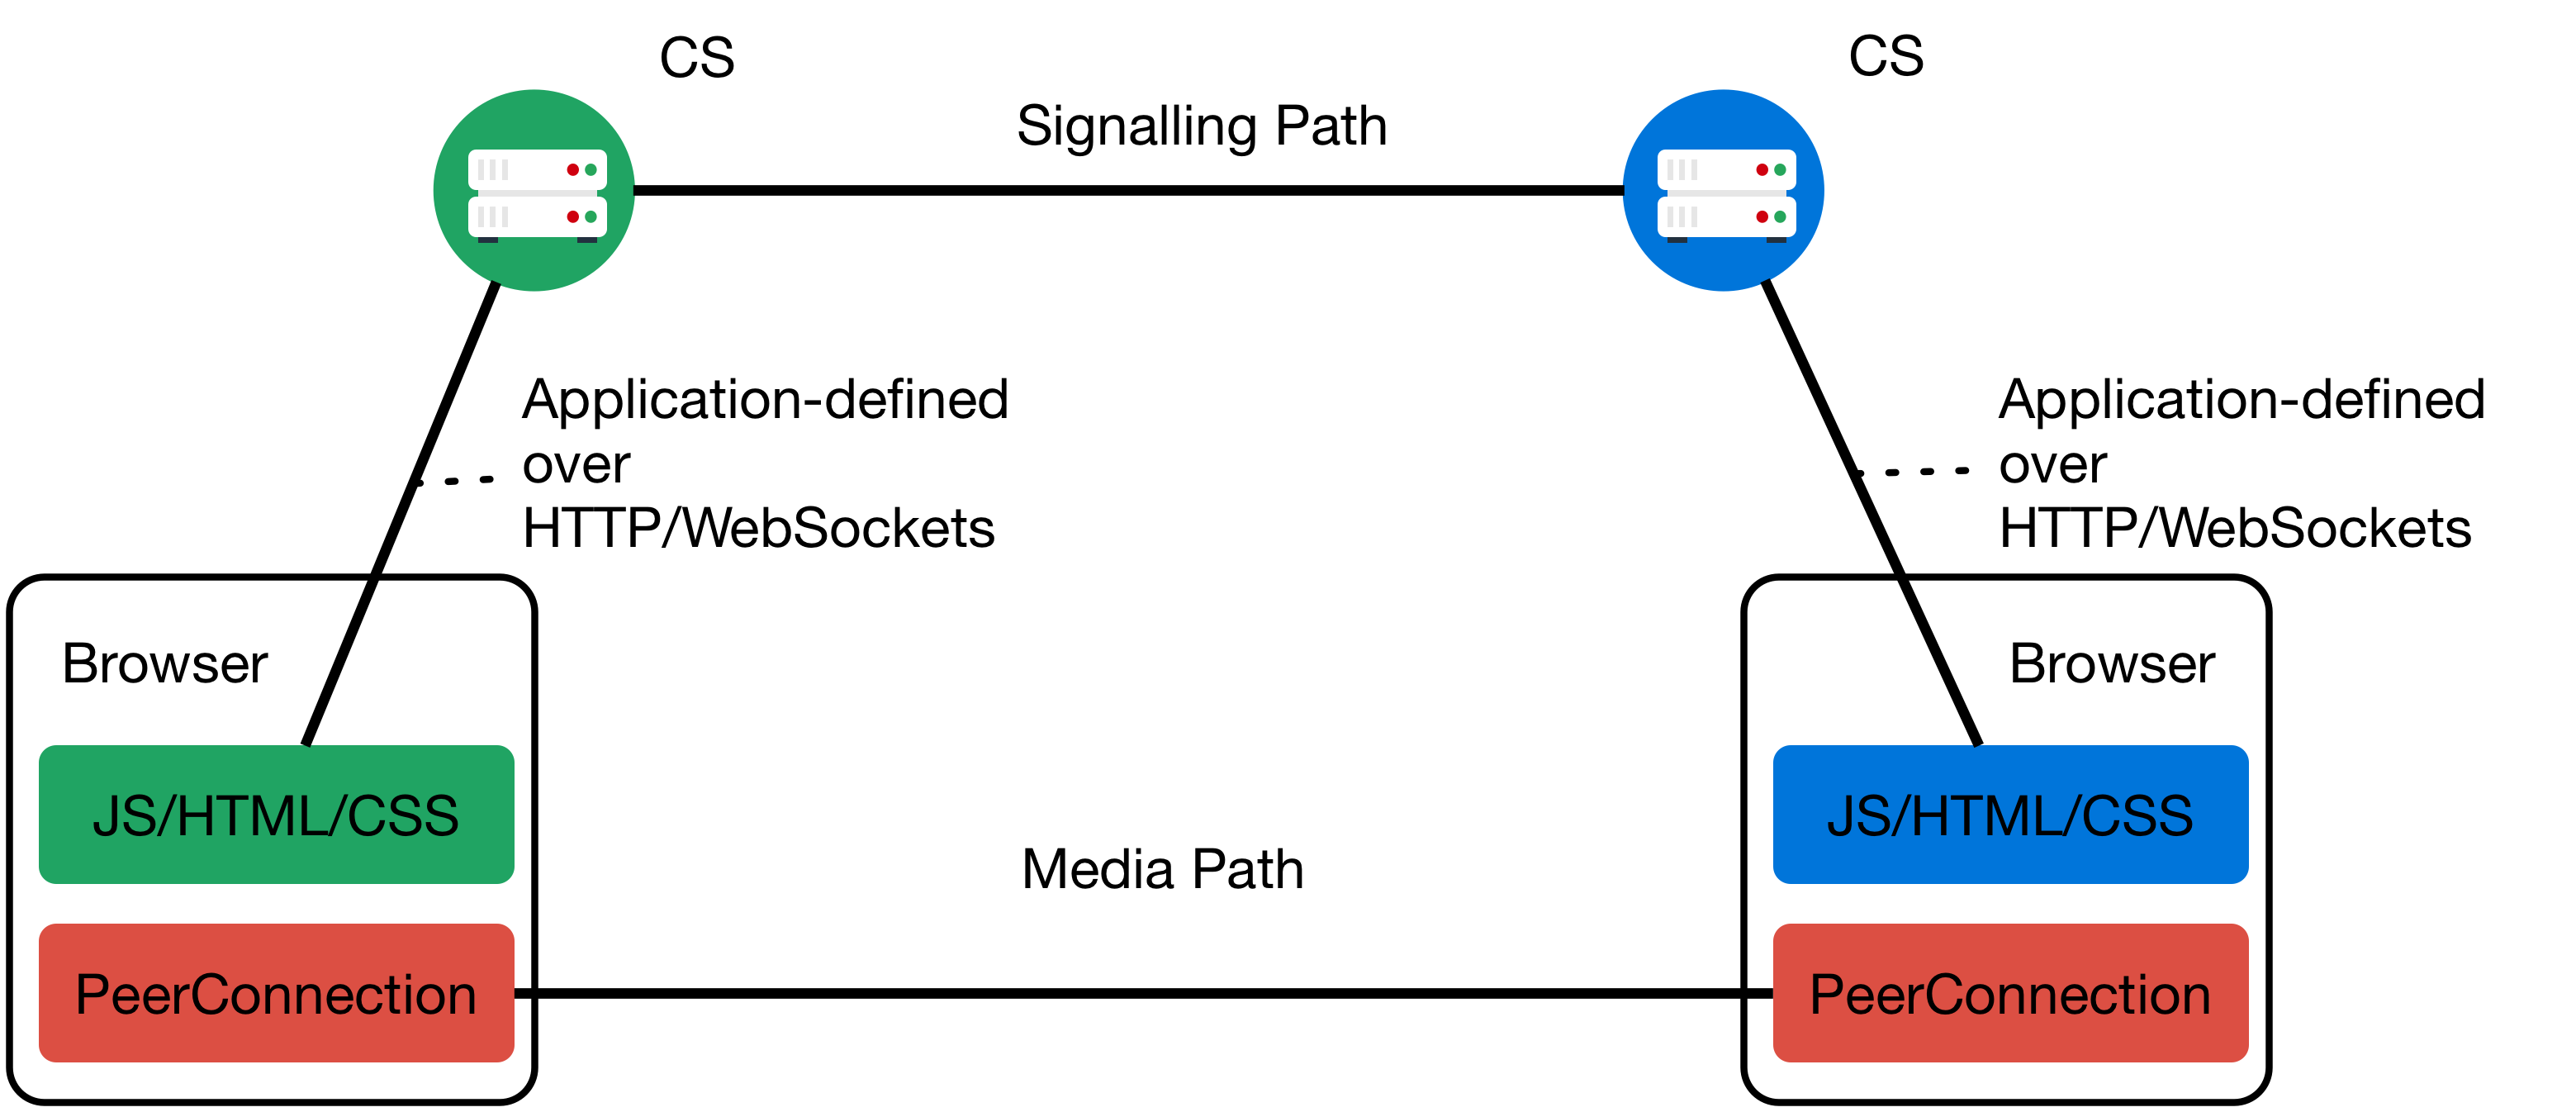
\includegraphics[width=.9\textwidth]{images/webrtcDeployment}
\caption{WebRTC deployment with two browser endpoints and two signalling servers~\cite{I-D.ietf-rtcweb-overview}.}
\label{fig:webrtcsig}
\end{figure}


\marginpar{
\captionsetup{type=figure}
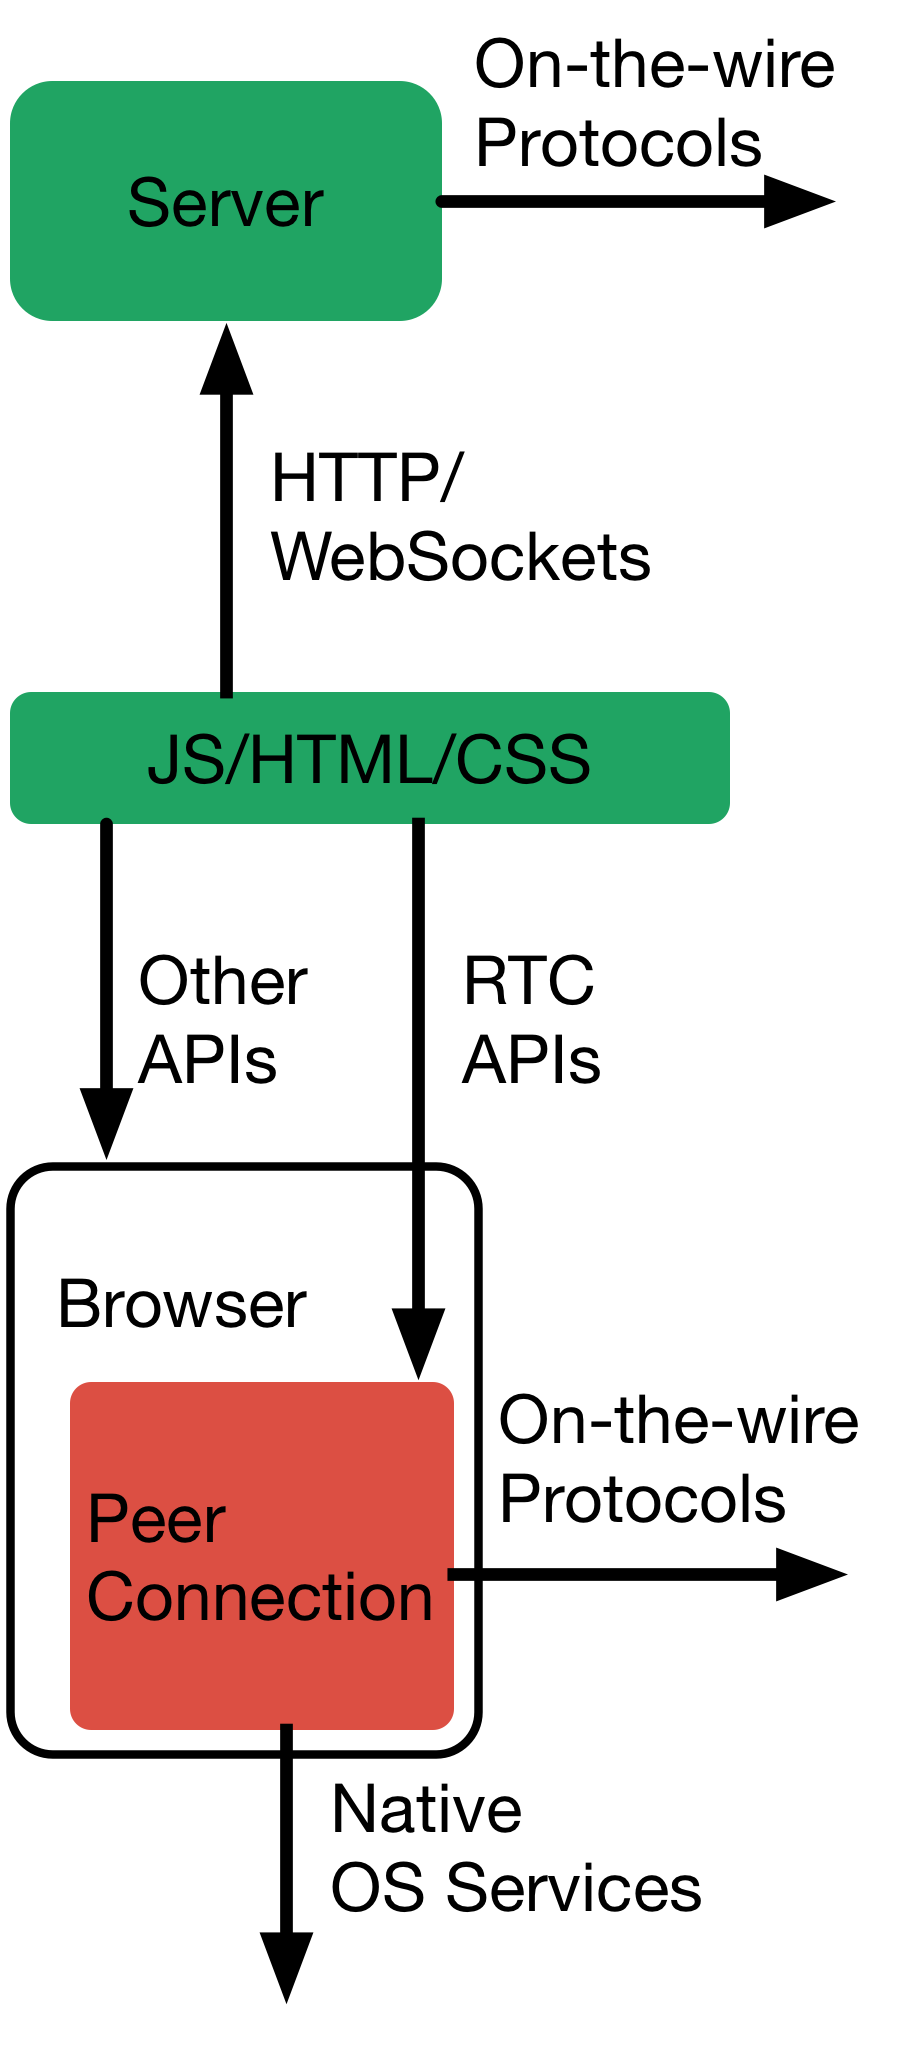
\includegraphics[width=\marginparwidth]{images/webrtcEndpoint}
\caption{WebRTC browser endpoint model~\cite{I-D.ietf-rtcweb-overview}.}
\label{fig:webrtcbrowser}
}


The main interface exposed by the WebRTC \gls{api} is the RTCPeerConnection~\cite{w3c:webrtc}.
It exposes functions to the webpage's JavaScript allowing it to manage the WebRTC session and signalling.
The \gls{jsep} \gls{ietf} draft~\cite{I-D.ietf-rtcweb-jsep} describes how the RTCPeerConnection is used.
\gls{jsep} permits the establishment and control of a WebRTC session through the exchange of session description messages, in a simple offer/answer negotiation mechanism.
When an offer/answer exchange is required, the initiating endpoint calls the \texttt{createOffer()} function. 
The resulting offer is installed as a local configuration, using \texttt{setLocalDescription()}, and transmitted on the signalling path.
When received, the offer is used as a remote configuration, with the \texttt{setRemoteDescription()} interface.
Finally, the process is reversed: the receiver generates an answer, applies it as a local configuration, and sends it.
On receiving the answer, the initiator installs it as a remote description, completing the initial setup.

Session description messages use the \gls{sdp}~\cite{RFC2327} syntax, as presented in Figure~\ref{fig:sdpsyntax}.
The \gls{sdp} syntax defines a list of parameters, identified by type letters and belonging to one of the description levels: the session description level, the time description level, and one or more media description level. 
The set of type letters is quite small and not extensible, however, extensions are possible through the use of \texttt{a=} attribute lines.

\begin{figure}
\begin{verbatim}
Session description
        v=  (protocol version)
        o=  (owner/creator and session identifier).
        s=  (session name)
        i=* (session information)
        u=* (URI of description)
        e=* (email address)
        p=* (phone number)
        c=* (connection information - not required if included in all media)
        b=* (bandwidth information)
        One or more time descriptions (see below)
        z=* (time zone adjustments)
        k=* (encryption key)
        a=* (zero or more session attribute lines)
        Zero or more media descriptions (see below)

Time description
        t=  (time the session is active)
        r=* (zero or more repeat times)

Media description
        m=  (media name and transport address)
        i=* (media title)
        c=* (connection information - optional if included at session-level)
        b=* (bandwidth information)
        k=* (encryption key)
        a=* (zero or more media attribute lines)
\end{verbatim}
\caption{Session Description Protocol syntax}
\label{fig:sdpsyntax}
\end{figure}
% after audio
%a=sendrecv
%a=fmtp:109 maxplaybackrate=48000;stereo=1;useinbandfec=1
%a=fmtp:101 0-15
%a=ice-pwd:cf1b0f7d3182718ee580de9a5bc68645
%a=ice-ufrag:495d215b
%a=mid:sdparta_0
%a=msid:{0e832fa8-b782-0549-9e9e-3a071487d5c6} 
%    {979b603a-395e-2941-aa8d-e2bc0ddb0033}
%a=rtcp-mux
%a=rtpmap:109 opus/48000/2
%a=rtpmap:101 telephone-event/8000
%a=setup:active
%a=ssrc:2196327089 cname:{17ce3841-2445-ba43-a3a7-60e428f22d43}

Figure~\ref{fig:sdpexample} shows an example of a (shortened) \gls{sdp} message for a WebRTC session.
It is an \gls{sdp} answer for a session with audio and video channels, respectively identified as \texttt{sdparta\_0} and \texttt{sdparta\_1}.
Declaration of these channels starts with a \texttt{m} line specifying the channel type, \eg \texttt{m=audio}.
In the \gls{sdp} offer/answer negotiation, peers have to agree on various parameters, for example, audio and video codecs.
In order to conduct the negotiation, an offer includes multiple supported parameters.
If compatible, the answerer accepts these parameters by including them in his answer.
Preceeding this example, the original offer proposed five codecs for the audio channel: \texttt{opus}, \texttt{telephone-event}, \texttt{G722}, \texttt{PCMU}, and \texttt{PCMA}.
Only two, \texttt{opus} and \texttt{telephone-event}, are included in the answer and thus accepted by the answerer.


\begin{figure}
\begin{verbatim}
v=0
o=mozilla...THIS_IS_SDPARTA-54.0.1 5897145307417630851 0 IN IP4 0.0.0.0
[...]
a=fingerprint:sha-256 33:B1:D7:4B:29:29:29:AA:87:01:47:B3:59:41:[...]5D
a=group:BUNDLE sdparta_0 sdparta_1
a=ice-options:trickle
a=msid-semantic:WMS *

m=audio 29188 UDP/TLS/RTP/SAVPF 109 101
c=IN IP4 74.125.39.43
a=mid:sdparta_0
a=candidate:0 1 UDP 2122252543 131.254.67.174 54163 typ host
[...]
a=candidate:20 1 UDP 8331263 74.125.39.43 29188 typ relay [...]
a=rtpmap:109 opus/48000/2
a=rtpmap:101 telephone-event/8000
[...]

m=video 29188 UDP/TLS/RTP/SAVPF 121
c=IN IP4 74.125.39.43
a=mid:sdparta_1
[...]
\end{verbatim}
\caption{Example of a SDP message (answer)}
\label{fig:sdpexample}
\end{figure}

In order to efficiently communicate in a \gls{p2p} fashion, peers use the \gls{ice}~\cite{RFC5245} to find which of their network interfaces are able to see each other.
Indeed, a computer may be connected to different networks through different interfaces.
In the \gls{ice} protocol, peers collect candidate addresses and exchange them during the \gls{sdp} negotiation in \texttt{a=candidate} attributes.
Each pair of local and remote candidates are then tested to find potential matching interfaces. 
In some situations, for example behind a \gls{nat}, a peer may not know his publicly visible address. 
\gls{stun}~\cite{RFC5389} is a client-server protocol used by a client to discover the binding between his source address and his reflexive transport address\footnote{NAT modify the source or destination of packets going through them. The reflexive transport address is the public \gls{ip} address and port created by the \gls{nat} closest to the \gls{stun} server.}.
\gls{stun} is a tool that may not work in some configuration, in particular, if both peers are behind \gls{nat} routers with endpoint-dependant-mechanisms for address attribution.
In that case, a relay can be setup using the \gls{turn}~\cite{RFC5766} extension to \gls{stun}.
Once ICE checks have completed, both peers can set up their secure channels.



%%%%%%%%%%%%%%%%%%%%%%%%%%%%%%%%%%%%%%%%%%%%%%%%%%%%%%
%%%%%%        WEB SECURITY
%%%%%%%%%%%%%%%%%%%%%%%%%%%%%%%%%%%%%%%%%%%%%%%%%%%%%%

\section{Security on the Web}
\label{sec:websecurity}
The World Wide Web, or more commonly the Web, is one of the many applications of the Internet.
It allows to retrieve and manipulate resources hosted by a server and referencing other resources by hypertext links.
The Web is built on a client-server model, and the most common type of client is, of course, the web browser.
Web clients are often referred to as user-agents, particularly in web specifications.

The set of protocols and specifications forming the Web are mainly defined by two standardisation bodies.
Languages such as HTML and CSS, protocols such as the \gls{http}, and web \gls{api} such as WebRTC \gls{api} are standardised by the \gls{w3c}~\cite{W3CStandard, W3CAPI}.
As the Web is built on the Internet, the \gls{ietf} contributes to protocol specifications which are then used in the context of the Web.
The \gls{ecma} is also an important actor as it standardises the ECMAScript programming language, better known under the name of Mozilla's implementation: JavaScript.
Browser makers, as the implementors of the most used web clients, are also central to the definitions, evolutions, and adoptions of web specifications.
The most important browser makers are Google (Chrome), Mozilla (Firefox), Microsoft (Edge/IE), and Apple (Safari). Figure~\ref{fig:w3schools} gives a rough indication of the balance of power between these main four browsers.
If a feature is not implemented or removed from one of the popular browsers it will soon be abandoned by websites.
Yet, implementing the full standard specifications is a daunting task and browsers, although regularly updated, often offer incomplete support for some features.
Keeping up with particular features and implementations from each browser is a complex task for website developers.
A common technique is to conditionally use \textit{shims} or \textit{polyfills}, adapter code that abstract browsers' implementations under a single interface.


\marginpar{
\captionsetup{type=figure}
\centering
\begin{tikzpicture}
\begin{axis}[
    ybar=0pt,
    ytick={0,25,50,75},
    axis y line*=none,
    axis x line*=none,
    tick label style={font=\footnotesize},
    legend style={font=\footnotesize},
    label style={font=\footnotesize},
    width=\marginparwidth,
    bar width=2.5mm,
    xtick=data,
    %xmin=-1,
    %xmax=2,    
    yticklabels={0\%, 25\%, 50\%, 75\%},
    xticklabels={w3school.com,gs.statcounter.com},
    xticklabel style={rotate=45},
    ymin=0,
    area legend,
    legend style={at={(1,1)},anchor=south east},
    y=.5mm,
    enlarge x limits={abs=0.5}
    %enlargelimits=false
    %enlarge y limits={abs=0.},
]
\addplot[ybar,matred,fill=matred] coordinates{(0,3.3)(1,14.2)};
\addplot[ybar,matblue,fill=matblue] coordinates{(0,4.6)(1,3.6)};
\addplot[ybar,matorange,fill=matorange] coordinates{(0,13.3)(1,6)};
\addplot[ybar,matgreen,fill=matgreen] coordinates{(0,76.3)(1,55.7)};

\legend{Safari, Edge/IE, Firefox, Chrome}
\end{axis}  
\end{tikzpicture}
\caption{Percentage of recorded browsers visiting \protect\url{w3schools.com} and \protect\url{amiunique.org} in June 2017.}
\label{fig:w3schools}
}

\subsection{The Trusted Computing Base}
\label{sec:tcb}
The \gls{tcb} is the set of hardware and software on which the security of a system relies upon.
In a correct implementation of a \gls{tcb}, if a part of the \gls{tcb} is compromised, then the whole system's security may be at risk.
However a compromised component not part of the \gls{tcb} should not present a risk to the security of the system in general or to any other components in particular.
While from an \gls{os} point of view the browser is just an application outside of the \gls{tcb}, in the context of the Web the browser is a central part of the \gls{tcb}. 

In other words, the browser can actually be considered as the \gls{os} of the Web.
Indeed, it is responsible for downloading and running client web application, while exposing resources and services through web \gls{api}.
As other \gls{os}, the browser is also responsible for maintaining applications isolation.

\subsection{The Same Origin Policy}
For web applications, isolation relies on the concept of origin and the same-origin policy~\cite{RFC6454}.
An origin is a protection domain regrouping \gls{uri}~\cite{RFC3986} sharing the same triple of scheme, host, and port.
Two pages from different origins are isolated and cannot share resources, such as variables or cookies.
However, communication is still possible using the postMessage \gls{api}.
This interface allows pages from different origins to exchange scoped message and cloned variables.

\begin{figure}
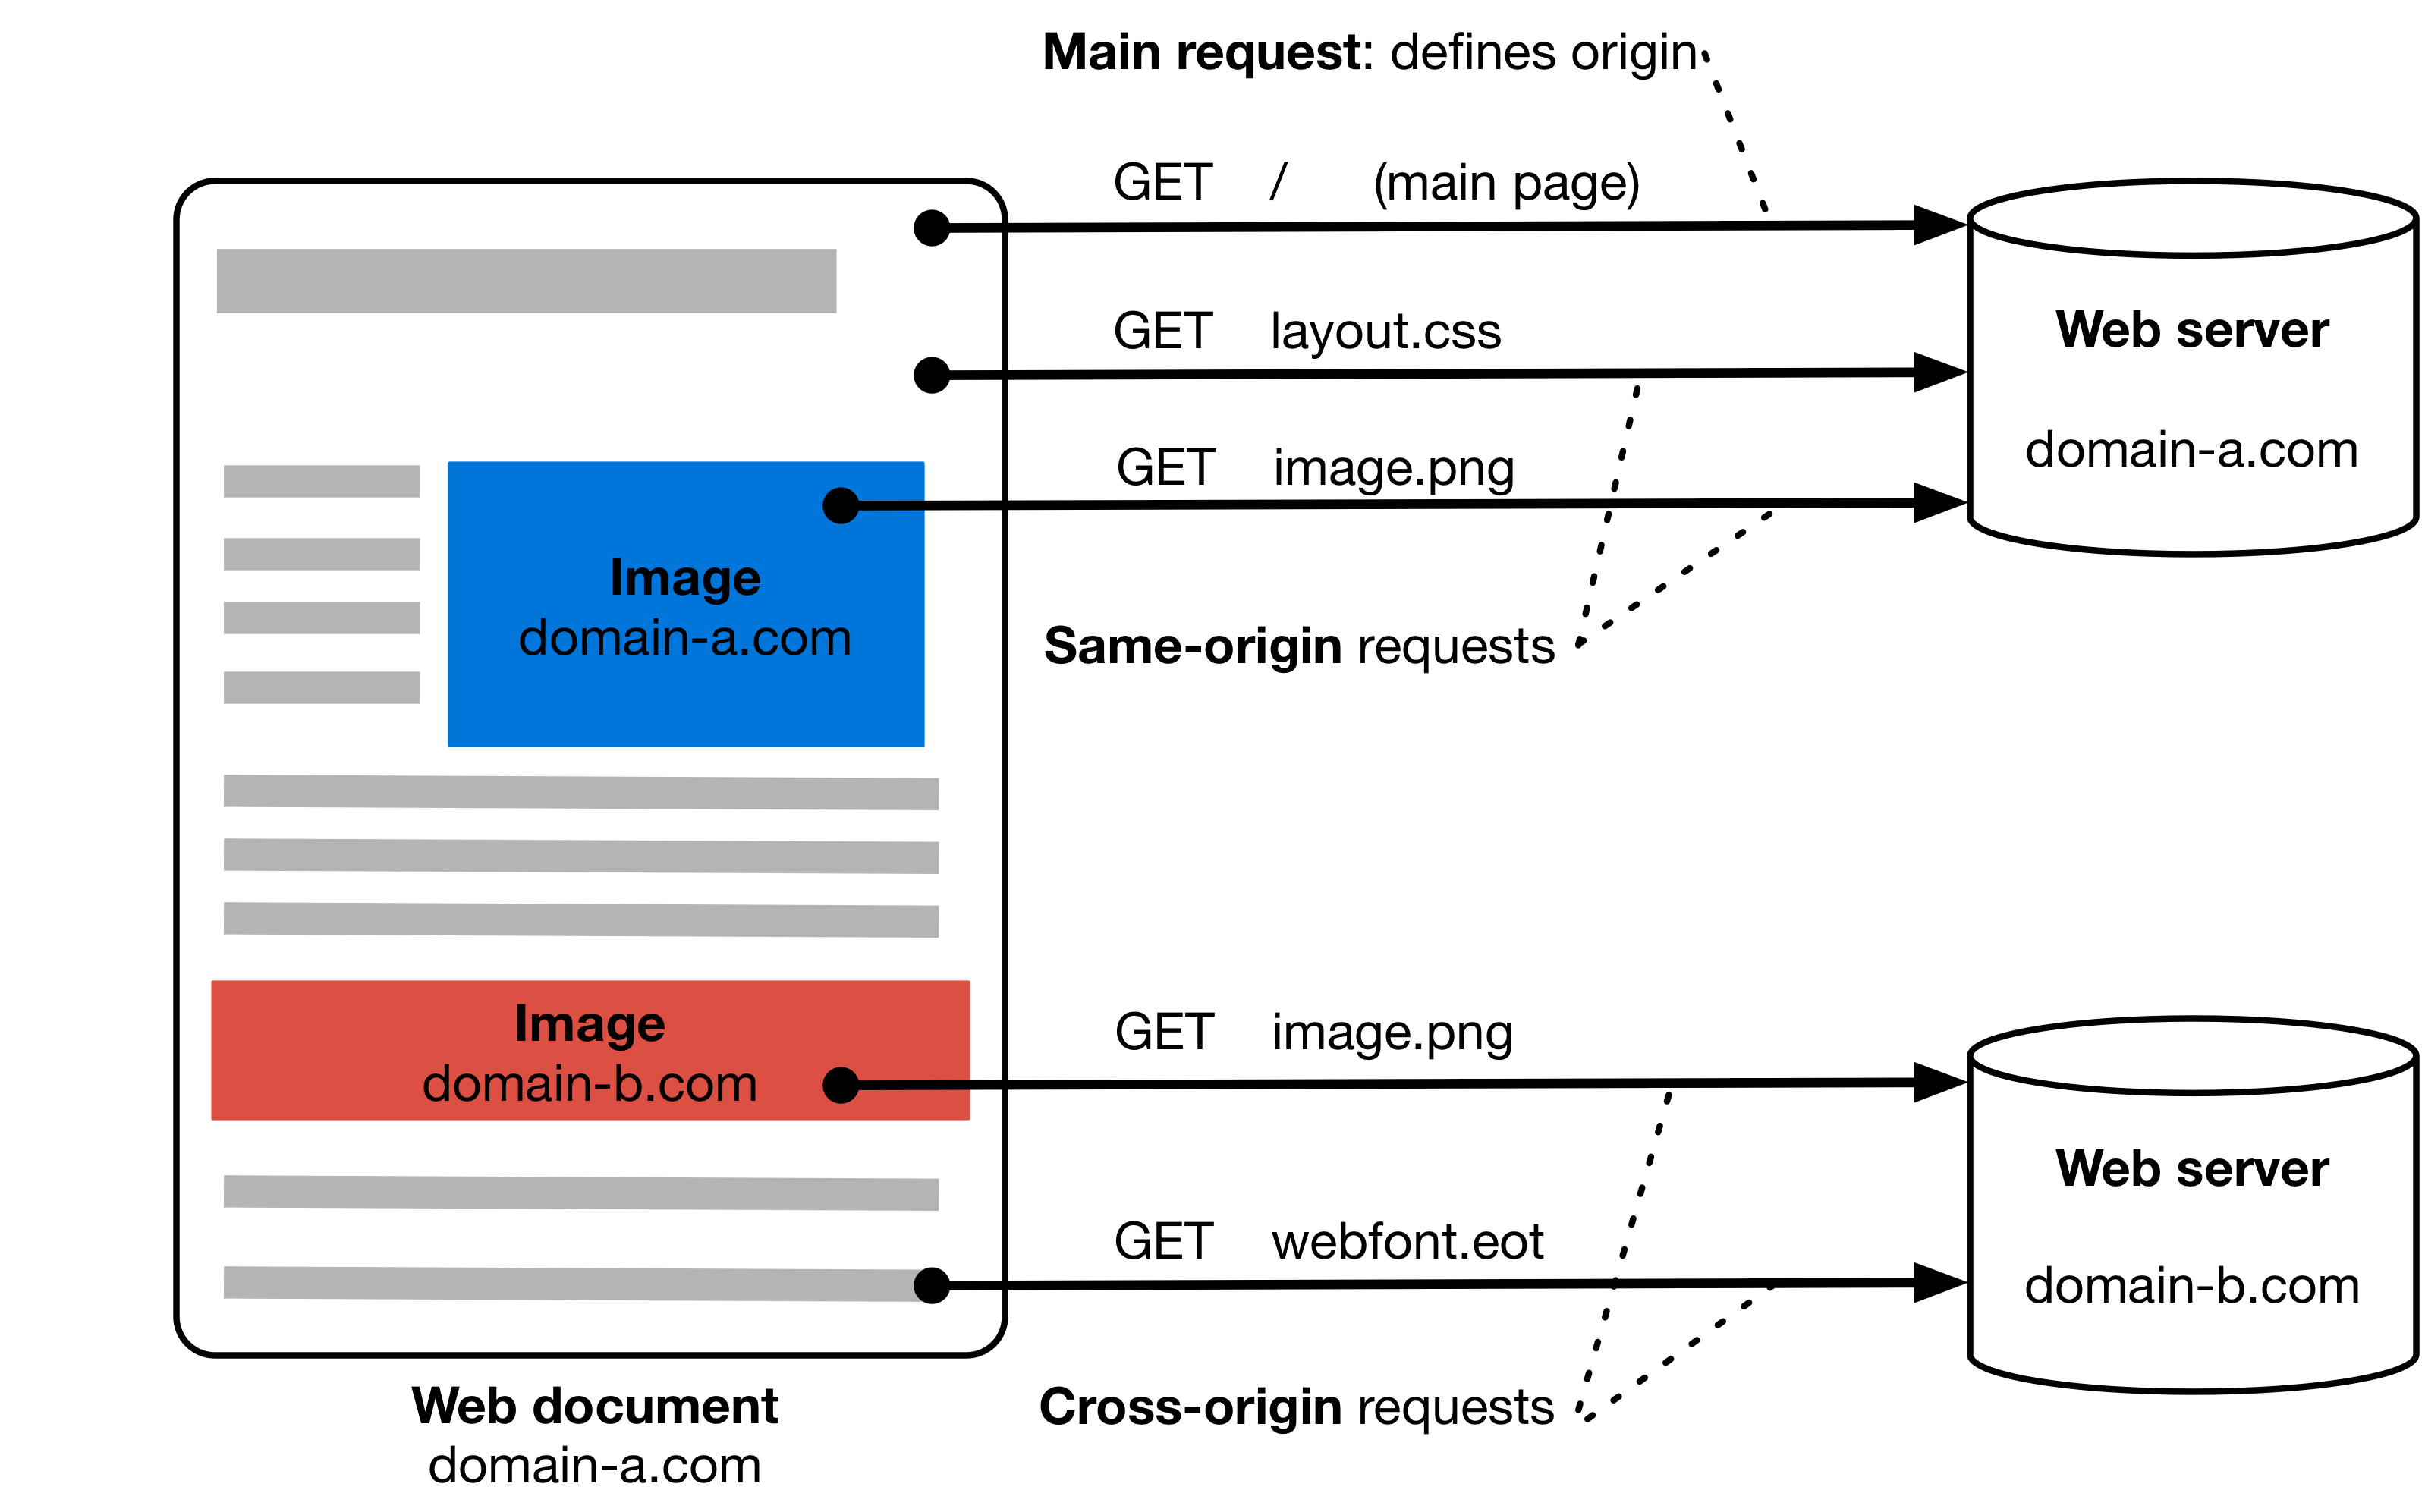
\includegraphics[width=\textwidth]{images/CORS}
\caption[Cross-site Request Example]{Cross-site request example. The HTML page from \protect\url{domain-a.com} requests resources from \protect\url{domain-a.com} and \protect\url{domain-b.com}. Requests for \protect\url{domain-a.com} are same-origin and always allowed. Requests for \protect\url{domain-b.com} are cross-origin and requires valid CORS headers and CSP directives. Example taken from \protect\url{developer.mozilla.org}.}
\label{fig:cors}
\end{figure}

A web application can also embed contents such as scripts or images from other origins. 
Figure~\ref{fig:cors} shows an example of a webpage with content loaded from two different domains.
Cross-origin content may enable vulnerabilities in a webpage as it enables the coexistence of two origins in a single security-context.
\gls{xss} and others code injection attacks exploit the user's trust in a webpage.
This kind of privilege escalation attack allows a malicious script to gain access to sensitive session information from the security context of the main origin.
One way for a webpage to prevent \gls{xss} is to define whitelisted origins through the use of \gls{csp} directives~\cite{9524886}.
This ensures that only trusted content can be loaded and executed by the web application.
Unlike \gls{xss} attacks, \gls{csrf} attacks exploit a web application's trust in a user's authentication to issue commands in place of the user.
To issue a \gls{csrf} attack a malicious webpage visited by the user executes an illegitimate \gls{http} request on the vulnerable server.
The request may, for instance, be triggered by loading a link inside an HTML image element or the execution of a JavaScript fetch request.
Supposing that the user is authenticated on the vulnerable application the illegitimate request inherits from this authentication, for instance through a session cookie.
Web applications may deter \gls{csrf} attack by enforcing the same-origin policy for some of their exposed \gls{http} interface.
This can be achieved by setting unique and unpredictable csrf-token cookie on the client side, or by defining \gls{cors}~\cite{RFC6454} headers on \gls{http} responses.
In both types of attacks, \gls{csrf} and \gls{xss}, the browser is responsible for correctly applying policies defined by web applications in order to protect the user.

Web-based protocols may require the discovery of policy or configuration information through metadata.
In order to avoid collisions with existing resources but also prevent impersonation on self-hosting services, \gls{rfc} 5785~\cite{RFC5785} defines well-known \gls{uri}.
A well-known \gls{uri} is a \gls{uri} whose path components starts with \texttt{/.well-known/}.
Specifications often define resources located under a well-known \gls{uri} and assume that they are under control of the host.


\subsection{The HyperText Transfer Protocol Secure}
\label{sec:https}
\glsreset{http}
\glsreset{tls}
\glsreset{https}
The \gls{http}~\cite{RFC2616} is an Internet application layer protocol~\cite{RFC1122} developed to access and modify web resources.
It offers several methods to send resource requests from a client to a server.
The two main ones are GET which is used to retrieve a resource, and POST which is used to send data to the server for creating or updating a resource. 
Responses to \gls{http} requests are made of a status code and an eventual body containing the actual response, \eg a file or an object.
For instance, the status code 200 means that the request is successful while the set of 300 codes indicates a redirection.

\gls{https}~\cite{RFC2818} is the combination of the \gls{http} and \gls{tls}~\cite{RFC5246} protocols\footnote{Note that as HTTP is not considered secure, HTTP and HTTPS page from the same domain are not considered to be from the same origin.}.
\gls{tls} enables authentication and secure communication between a client and server\footnote{Although client authentication is also possible with TLS, it is not much used and often limited to server-server interactions or other particular use cases.}. 
To authenticate itself to a client a server must provide a signed and valid certificate containing, in particular, his public key, his domain name, and the certification authority which issued the certificate.
After the client validated the certificates, it uses the public key to communicate a secret session key to the server initiating a secure communication between both parties.

Certification authorities are the entities responsible for issuing and signing certificates.
There exist four types of \gls{https} certificates ranging from self-signed certificates to Extended Validation certificates.
These types differ from the verification conducted by certification authority, their costs, and the way they are displayed by browsers.
Although there is debate whether Organisation Validation certificates offer more guarantees as Domain Validation certificates.
Some Extended Validation certificates are integrated by browser makers within their browser installation packages.
These are often referred to as root certificates as they do not depend on other certificates.
It is the responsibility of the browser makers to select trustworthy certification authority for providing root certificates.

In addition to initialising trust chains, the responsibility of the browser is to provide security information to the user when they connect to a website.
This is usually done by displaying a colour coded indications of the page security level in the address bar and in-context warning such as in Figure~\ref{fig:httpssecurity}.
Mixed contents such as an insecure login forms are also taken into account to determine the security level.
However, if the certificate is invalid the page is automatically blocked by the browser.
While this effectively deters attacks, users usually only see false alarms~\cite{herley2009so} which could, in turn, have the effect of lowering their vigilance.

Browser makers are currently pushing \gls{https} and advocating for a fully encrypted Web.
For instance, Firefox indicated that they will advertise \gls{http} site similarly to bad certificate~\cite{mozillasecurityblog2017communicating}. 
A full \gls{https} web would lower the trust of users in \gls{http} websites, and force those site to finally adopt \gls{https}.
This objective is made possible thanks to automated \gls{ca} such as Let's Encrypt which operates the \gls{acme} protocol.
Let's Encrypt aims at drastically reducing the complexity and cost of certificate deployment by avoiding manual operations, a major barrier for the multitude of small websites.
Ultimately, the usage of \gls{https} is not a proof of trustworthiness of the website itself but only that the control of its domain name was verified to some extent and that secure communication is in place.

\marginpar{
\captionsetup{type=figure}
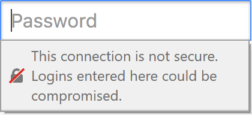
\includegraphics[width=\marginparwidth]{images/firefox_warning}\\\\
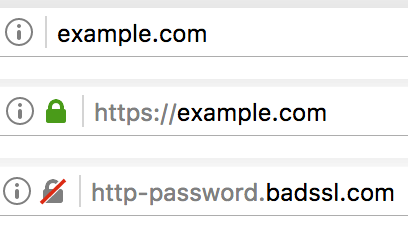
\includegraphics[width=\marginparwidth]{images/httpslevel}
\caption[Web Browser Security Indications]{Security indications for HTTP, HTTPS and insecure password form on Firefox. The HTTP indicator will soon be replaced by a warning similar to the example shown here.}
\label{fig:httpssecurity}
}

\subsection{Public Key Cryptography}
\label{sec:pubkey}
This section introduces the notion and usages of public key cryptography, a corner-stone of the security of the Web.
This technique allows to sign, authenticate, and secure messages exchanged by two peers without the need to share a common secret key.
Public key cryptography is used in the certificate infrastructure deployed by browsers and \gls{ca} for \gls{https}, but also in the WebRTC security protocols, and in authentication delegation protocols.


In 1976 Diffie and Hellman published the concept of public key cryptography, also called asymmetric cryptography.
The race for such an algorithm was won by Ron Rivest, Adi Shamir, and Leonard Adleman with the publication of the famous RSA algorithm.
In symmetric cryptography, the same key is used to encrypt and decrypt the message. 
This is, for instance, the case with Caesar's cypher where the key is the number of shifts to apply in order to encrypt a plaintext message, but also the number of opposite shift to decrypt the message. 
Conversely, public key cryptography protocols use two keys.
The secret key is randomly generated while the public key is derived from the secret key, both forming a key pair.
As knowledge of the public key does not allow to retrieve the private key, the public key can be shared freely.
We do not go into details on the specific cryptography mechanisms and algorithms but focus on the use cases made possible by asymmetric cryptography.

In order to bind an identity to a key pair, a \gls{ca} issues a digital certificate.
These certificates contain information about the public key, the signing algorithm, the owner's identity, and the \gls{ca}.
Certificates may also refer to the \gls{ca}'s own certificate until a trusted root certificate is reached forming a chain of trust.
X.509 certificates, one of the most used standards for digital certificates, contain several fields describing the certificate itself, the issuer, and the subject.
An example is given in Figure~\ref{fig:x509}.
Another way to issue certificates is to participate in a web of trust where members respectively sign their keys during key exchange party.
OpenPGP~\cite{RFC4880} is the most widely used web of trust standard, particularly for signing emails.

\begin{figure}
\begin{tabular}{@{}ll@{}}\toprule\toprule
   \textbf{Subject} & \\
   Common Name & energyq.idp.rethink.orange-labs.fr \\\midrule
   \textbf{Subject's Public Key} & \\
   Public Key Algorithm & PKCS \#1 RSA Encryption \\
   Public Key & c5 44 1c 33 79 bf e5 [...] c9 26 a4 e3 5e 4e 6d\\\midrule
   \textbf{Issuer} & \\
   Common Name & Let's Encrypt Authority X3 \\\midrule
   \textbf{Period of Validity} & \\
   Begins On & 31 mai 2017 \\
   Expires On &  29 ao�t 2017\\\midrule
   \textbf{Fingerprints} & \\
   Signature Algorithm & PKCS \#1 SHA-256 With RSA Encryption \\
   SHA-256 Fingerprint &  77:21:3C:64:0A:ED:E3:AD:0F:82:03:6D:9B:45:66:B4:\\ & D0:28:D8:04:9E:F3:41:C1:C7:A5:EA:57:BB:A0:34:1D\\\bottomrule
   \hline
\end{tabular}
\caption[X.509 Certificate]{Extract of a X.509 certificate issued by Let's Encrypt to energyq.idp.rethink.orange-labs.fr. }
\label{fig:x509}
\end{figure}

\begin{figure}[H]
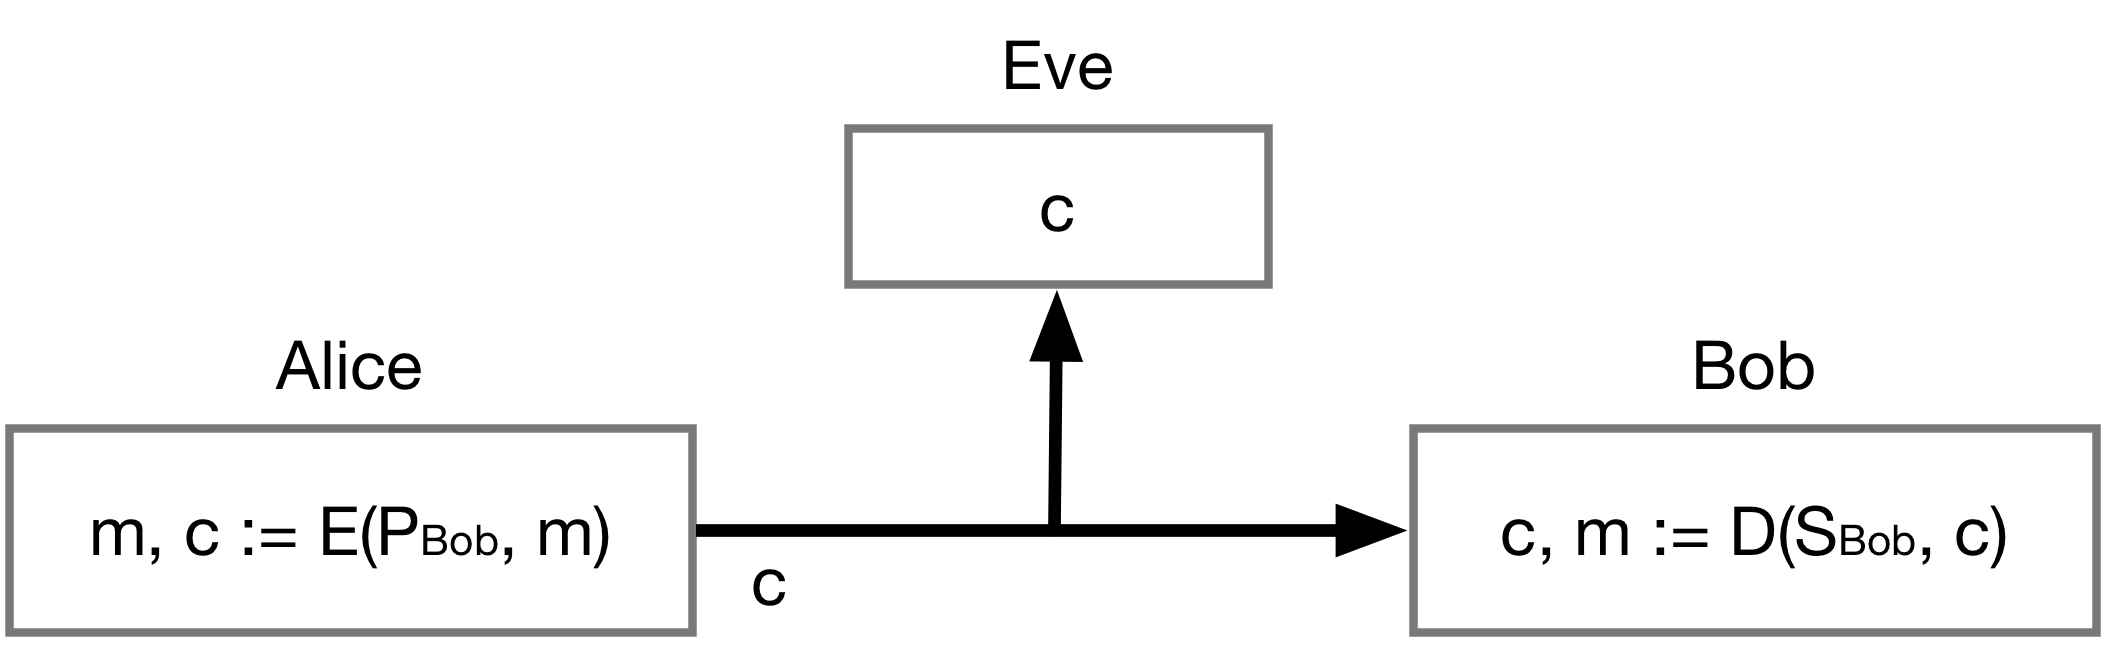
\includegraphics[width=.7\textwidth]{images/encrypt}
\caption{Public-key encryption of $m$ from Alice to Bob~\cite{ferguson2011cryptography}.}
\label{fig:symenc}
\end{figure}

In the public key encryption scenario (Figure~\ref{fig:symenc}), Alice wants to send an encrypted message $m$ so that it is only readable by Bob, the intended recipient.
Bob possesses a key pair $(P_{Bob}, S_{Bob})$ and publishes its public key.
Alice then uses this public key to encrypt the message and send the cyphertext to Bob.
On receiving the encrypted cyphertext, Bob uses its secret key to decrypt the message.
While the attacker Eve could not read the cyphertext, it could still intercept the message and modify it. 
Confidentiality is ensured, but encryption does not prove message integrity nor the sender's authenticity.


\begin{figure}[H]
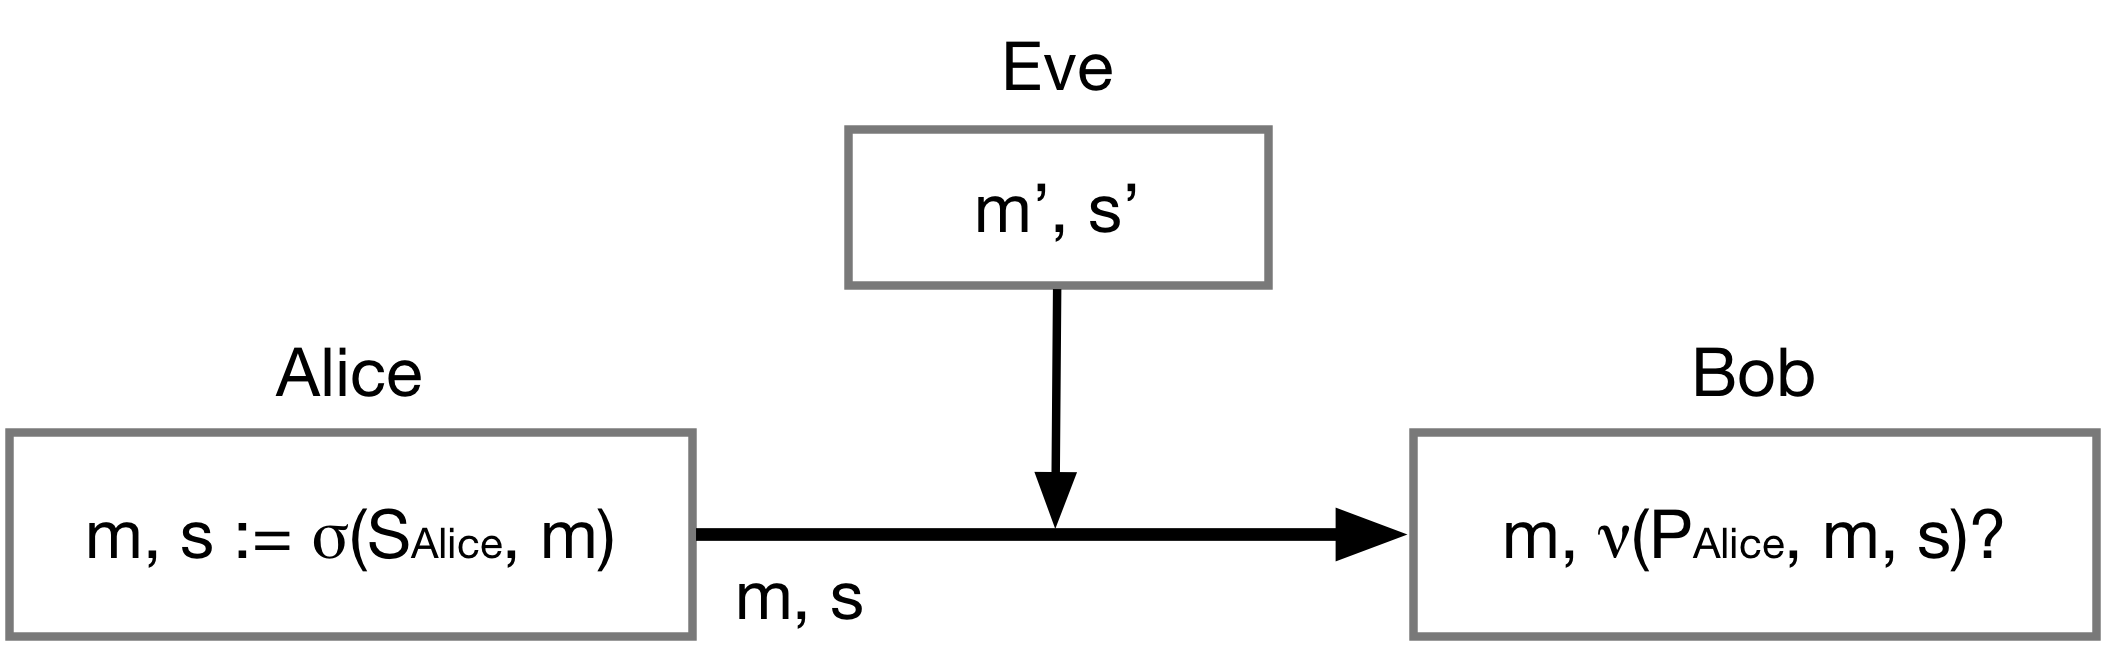
\includegraphics[width=.7\textwidth]{images/signature}
\caption{Public-key signature of a message $m$ from Alice to Bob~\cite{ferguson2011cryptography}.}
\label{fig:symsig}
\end{figure}

In the signature scenario (Figure~\ref{fig:symsig}), Alice possesses a key pair $(P_{Alice}, S_{Alice})$ and publishes its public key.
In order to sign a message $m$, Alice uses a signing algorithm with the private key and the plain text as a parameter to produce a tag, \ie the signature $s$.
She then sends both plain text and signature to the recipient.
The signature algorithm is often associated with a cryptographic hash function, a one-way function mapping the message to a fixed size string.
In this case, the signature is applied on the resulting hash, also called a digest.
By verifying the signature with the public key and comparing it to the message, or the message's digest, the receiver is then able to verify the integrity of the received message.
Only the holder of the secret key could have produced the signature.
If the key pair is bound to the sender's identity, for instance with a certificate containing the sender's name, the receiver also verifies the authenticity of the message.

Achieving both confidentiality and integrity is possible if both parties publish their respective public keys.
To do so the sender would sign the message with its own private key and then encrypt both message and signature with the other party's public key.
Using asymmetric encryption is, however, a computationally heavy operation compared to symmetric encryption. 
In order to solve this problem, public key cryptography is used to establish a symmetric session key.
Such key exchange scheme is often referred to as a Diffie-Hellman exchange.

A cypher suite is a standardised configuration of cryptographic algorithms and options meant to serve as a toolbox for establishing a secure communication.
In \gls{tls}, a cypher suite would define the key exchange algorithm, the bulk encryption algorithm, the signature algorithm and the relevant key size to be used.
Prior to starting the negotiation, both peer would make a hand-shake to compare their respective available cypher suite and find a common ground.
Figure~\ref{fig:cyphersuit} shows the cypher suit used on \url{idp.energyq.rethink.orange-labs.fr} with Firefox.

\marginpar{
\captionsetup{type=figure}

\footnotesize{\textbf{TLS\_ECDHE\_RSA\_\\WITH\_AES256\_GCM\_\\SHA384}}
\caption[Cypher Suit Example]{This cypher suit defines ECDHE as the key exchange mechanism, RSA as the authentication mechanism, AES\_256\_GCM as the symmetric encryption algorithm, and SHA384 as the digest algorithm.}
\label{fig:cyphersuit}
}


%%%%%%%%%%%%%%%%%%%%%%%%%%%%%%%%%%%%%%%%%%%%%%%%%%%%%%
%%%%%%        WEBRTC SECURITY
%%%%%%%%%%%%%%%%%%%%%%%%%%%%%%%%%%%%%%%%%%%%%%%%%%%%%%
\section{WebRTC Security}
\label{sec:webrtcid}

While the signalling path is secured as any other client-server connection on the Web.
The media path serves for real-time media communications and as such uses different protocols.
Figure~\ref{fig:stack} shows the protocol stack for the WebRTC signalling and media path.
WebRTC mandates the use of secure media channels\footnote{A consistent decision with the direction for HTTPS everywhere.}~\cite{I-D.ietf-rtcweb-security-arch}.
In this section we present the protocols protecting confidentiality, integrity, and availability of the media channel.
The WebRTC security architecture also introduces an optional identity path to let users verify their peer's authenticity.
We give definitions related to user authenticity in Section~\ref{sec:authn} and present the WebRTC Identity Path in Section~\ref{sec:webrtcidpath}.
We also give an overview of some alternative key management protocols in Section~\ref{sec:keymanagement}.

\begin{figure}
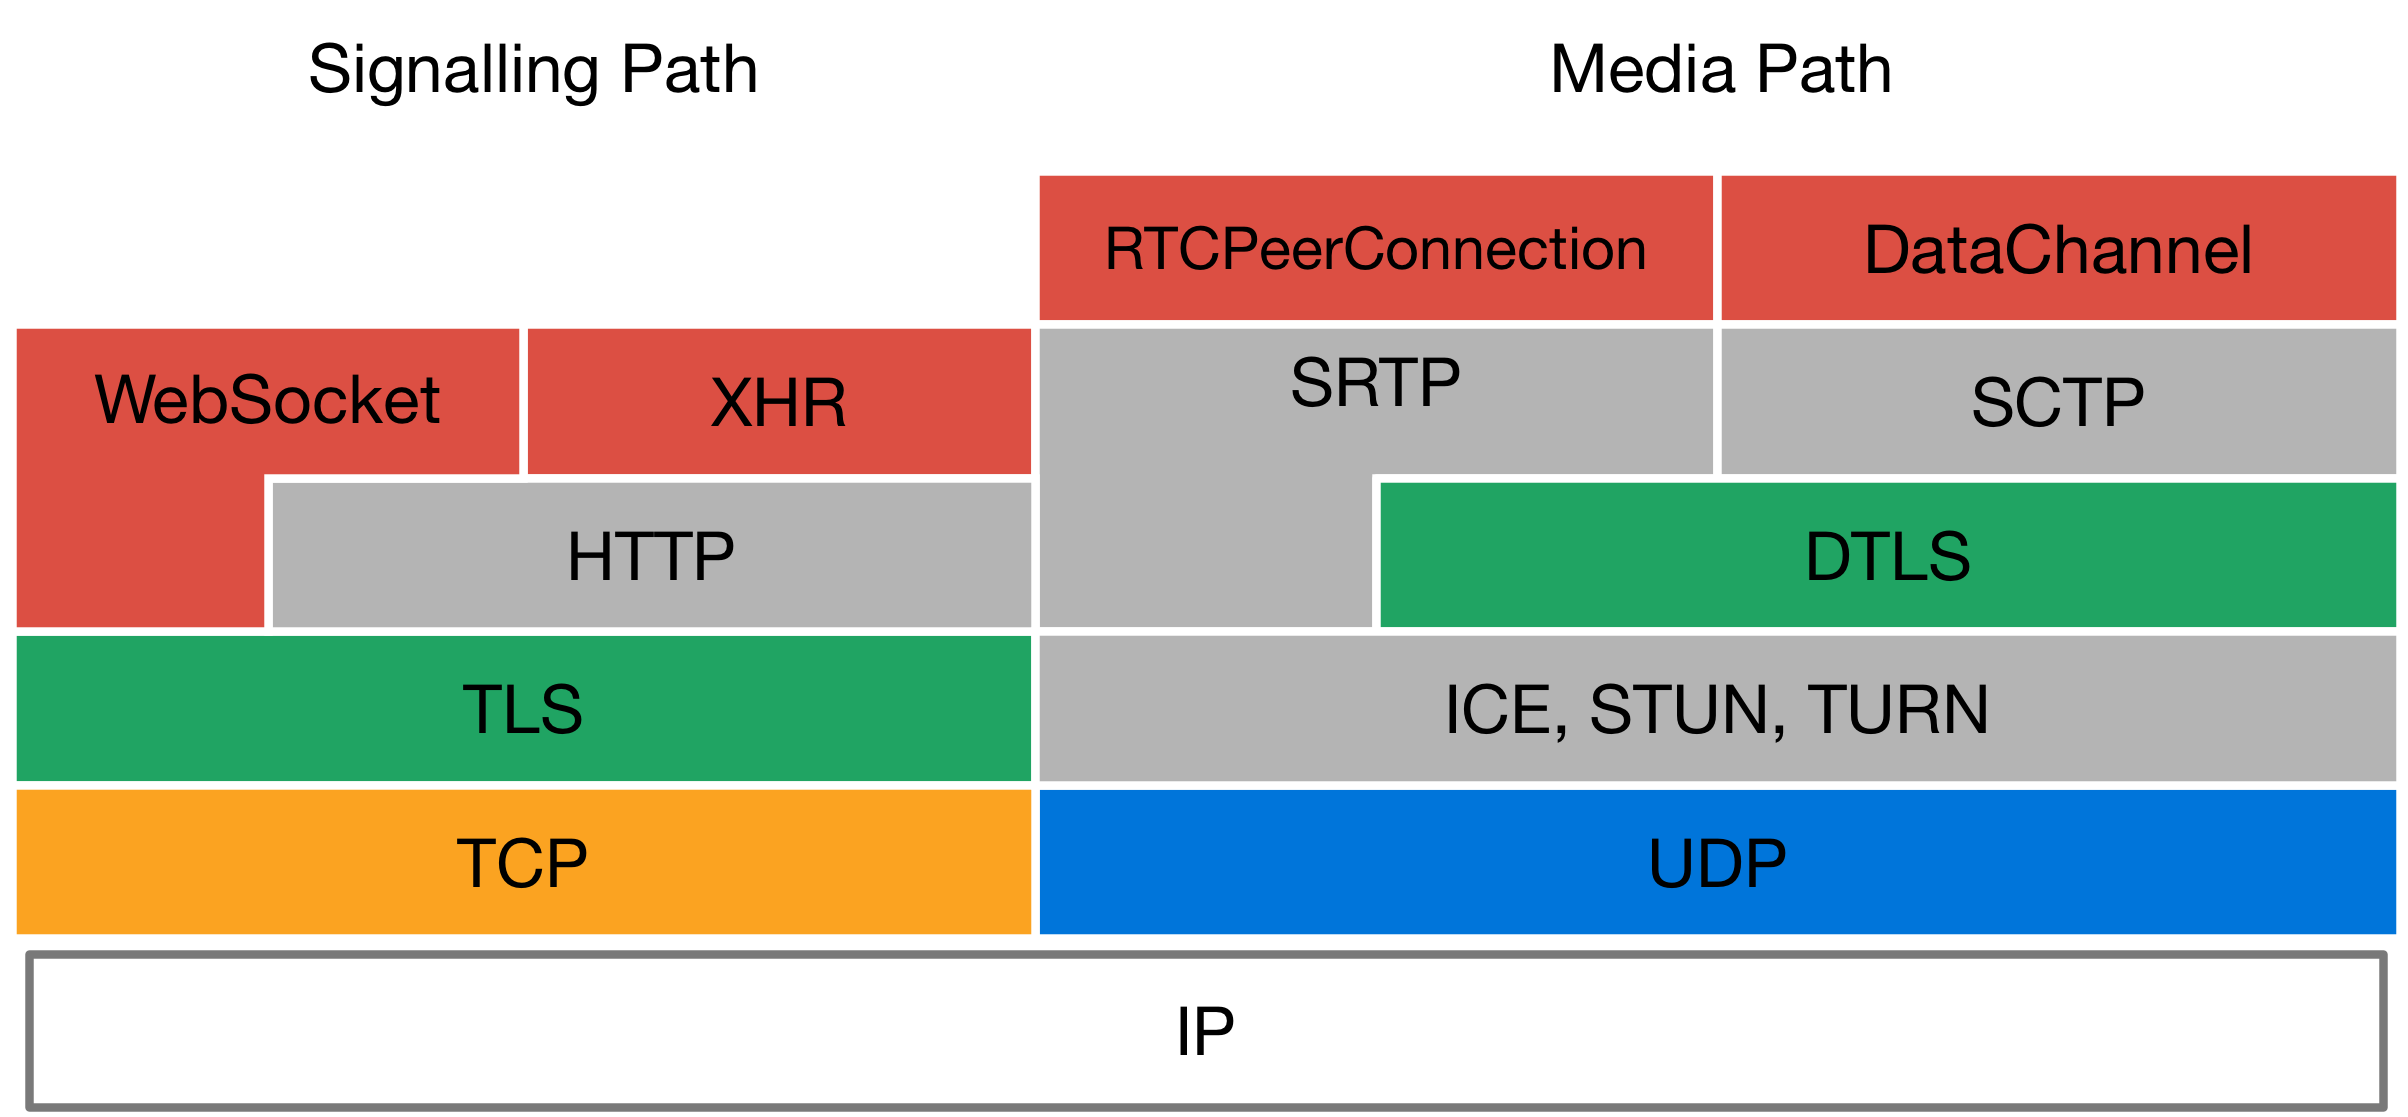
\includegraphics[width=.8\textwidth]{images/webrtcStack}
\caption{WebRTC Protocol Stack~\cite{HPBN}.}
\label{fig:stack}
\end{figure}

\subsection{Confidentiality and Integrity of the Media Path}
The media path is a \gls{p2p} connection between two WebRTC endpoints.
This path allows both the setup of media streams offered by the Media Capture and Streams \gls{api} or data channels from the RTCDataChannel \gls{api}.

\glsreset{srtp}\glsreset{rtp}\glsreset{rtcp}\glsreset{srtp}
Media streams are transported over the \gls{srtp}~\cite{RFC3711}, a secure profile for the \gls{rtp}~\cite{RFC3550} and \gls{rtcp} ``which can provide confidentiality, message authentication, and replay protection''.
Usually, the \gls{rtp} protocol (and \gls{srtp}) is carried over the \gls{udp}~\cite{RFC768} as real-time media streams are time-sensitive\footnote{Contrary to the \gls{tcp}~\cite{RFC793}, UDP does not guarantees the delivery, ordering, or duplicating of its packets and avoids the overhead of such guarantees.}.
As \gls{srtp} does not offer key management functionality, it must rely on another key management protocol.
The preferred and default protocol for \gls{srtp} key management is the \gls{dtlssrtp}~\cite{RFC5763} which must be offered by any WebRTC implementation.
\gls{dtls}~\cite{RFC6347} is an adaptation of \gls{tls} to datagram transport protocols.
\gls{dtlssrtp}~\cite{RFC5764} is ``a \gls{srtp} extension for \gls{dtls} that combines the performance and encryption flexibility benefits of \gls{srtp} with the flexibility and convenience of \gls{dtls}-integrated key and association management''.
\gls{dtlssrtp} can thus be seen as a \gls{dtls} optimisation for \gls{rtp}.
On the other hand, data channels use the \gls{sctp}\footnote{SCTP can be configured to provide similar features to UDP or TCP.}~\cite{RFC4960} and are secured by \gls{dtls} only.

In order to exchange their public keys and setup a session key, peers proceed to a \gls{dtls} handshake over the media path by exchanging certificates.
Contrary to server exposing certificates signed by trusted \gls{ca}, peers' certificates are self-asserted and thus untrusted.
In order to authenticate the received certificates, fingerprints of these certificates are previously exchanged over the signalling path in session level \texttt{a=fingerprint} \gls{sdp} attributes (see Figure~\ref{fig:sdpexample} for an example).
As long as the signalling path is trusted, the confidentiality and integrity of the media path is ensured.


\subsection{Availability of the Communication}
\label{sec:availability}
The main threat to availability of a WebRTC communication consists in \gls{dos} attacks, and in particular \gls{ddos}.
As WebRTC calls are programmatically controlled, a malicious software could launch multiple calls from several users to a single destination, for instance a call-center.
The consent mechanisms required by the Media Capture and Streams \gls{api} mitigate these kinds of attack using media streams.
However, data channels do not require consent before being initialised and may be used to mount \gls{ddos} attacks.
Client applications and automated WebRTC implementations, \ie call-center gateway, should implement filtering policies to detect and respond to suspicious call, \ie call without audio or video.
The WebRTC security architecture~\cite{I-D.ietf-rtcweb-security-arch} details and reference additional availability attacks against WebRTC. 

More generally, WebRTC clients may also be vulnerable to \gls{spit}, \ie the transmission of bulk unsolicited call offers.
The possibility of WebRTC spam depends on the underlying signalling architecture.
For instance an open signalling federation would be more vulnerable to \gls{spit} than a one-way call service deployed on a website.
Nonetheless, there is few doubts that in the former case a spam agent would be easy to write.
\gls{rfc}~5039~\cite{RFC5039} references solutions to \gls{spit} call for \gls{sip} that could probably be adapted to WebRTC scenarios.
One solution proposed by the RFC is to implement white and black lists to automatically accept or reject incoming calls.
However, obtaining a new identity may be quite cheap making black lists ineffective. 

Finally, a WebRTC session may be impacted by the available bandwidth on the network.
Janczukowicz \etal\cite{JanczukowiczBTB16} demonstrate that concurrent \gls{tcp} flow may have an impact on the perceived quality of a WebRTC flow under best-effort routing.
Saturating a network path could thus be used to compromise the availability of the communication.
Alternative routing mechanisms could be used to provide specialised and paid communication services with a managed quality of service.
For instance using \gls{turn} servers for routing the media path, rather than using \gls{p2p} best-effort~\cite{JanczukowiczBTF15}.
However, specialised services on the internet are criticised by some as being against the philosophy of the Net Neutrality\footnote{The french \gls{arcep} published a state of the art report on net neutrality regulations and operators practices in September 2015~\cite{ARCEPNet}.}.


\subsection{User Authenticity}
\label{sec:authn}
For users navigating the Web, authentication is a common action involving an identifier and a password.
But it may be difficult for them to explain what are the authentication inherent concepts, and what precisely is their identity.
In the following paragraphs, we define and explain the concepts of identity, identifier, credentials, and claims.
We explain what constitutes an authentication process, and what makes it secure.

A subject's \textit{identity} is a set of attributes, called claims, representing the subject in a specific scope~\cite{identityCrisis}.
As an identity is only defined for a specific scope, and a subject may exist in multiple scopes, a subject may have multiple identities.
For instance, the claims described by a subject's driver license constitutes one of his identity. 
The same subject may also have a passport and some social network accounts.
Although these identities belong to the same individual and may overlap, for instance sharing the same name and age, they are distinct identities.

Identity is often used in the sense of an identifier~\cite{identityCrisis, usercentricity06}.
This confusion is due to the fact that a name, or a public identifier in digital identity, is often used as a synonym for an identity.
In the rest of our thesis, we will clearly make the distinction to avoid confusion.

\textit{Claims} are the attributes constituting an identity.
Identity claims can describe features of a user such as his name, his age, or his address.
But claims may also be used to grant access to resources.
In that case, we talk about authorization claims.
Though some of the claims on a driver license would be describing the driver itself, \eg \texttt{name:~Bob} or \texttt{age:~30}.
Some other claims may describe the category of cars the driver is authorized to drive, \eg \texttt{cat.~A: authorized}.
On the Web, an authorization claim may allow write and read access to some data or \gls{api}.
Claims are usually uniquely identified by a URI or reserved names defined by various standards.
For instance the OpenID Connect~\cite{sakimura_openid_2014} specification defines a set of standard identity claims.
As claims can change over time, an identity may also be dynamic.

An \textit{identifier} is a claim uniquely identifying the subject in a given scope.
Identifiers may have different forms such as a pseudonym, an email address, or a random text.
A website identifies the claimed identity by looking up its records and verifying if such identifier exists. 

\textit{Authentication} is the process by which an entity proves the validity of some claims to another party.
In the most common scenario, a user authenticates by claiming his identifier.
In this case, we say that the user authenticates himself (or just authenticates if unambiguous).
In order to prove the ownership of an identifier, \ie to authenticate, the user has to present valid \textit{authentication factors}.
Contrary to identifiers, authentication factors are not necessarily unique.
Indeed, several users may, by coincidence, use the same password. 
%However, these should be resistant to common attacks, as described in Section~\ref{later subsection}.\todo{define entropy for password}

Although authentication commonly refers to proving the ownership of an identifier, it is also possible to authenticate non-identifying claims.
%Pursuing data minimization (see Section~\ref{sec:privacy}), 
For instance, to protect its privacy a user may want to claim only his age without revealing his identifier.
In order to allow for this scenario, a trusted third-party is often necessary to assert the validity of claims.
However, identification remains possible if enough claims are provided.

In the most simple case, authentication is a simple relation involving two participants.
However, for privacy, usability, or security reasons, the process may be delegated to a trusted third party.
An \gls{idp} is a trusted authority issuing and validating identity claims.
The \gls{rp} is the consumer of identity claims.
Technically, claims are requested, obtained, and validated using authentication delegation protocols.
These protocols allow the exchange of claims through security tokens.
Depending on the protocol, the \gls{rp} requests some claims to an \gls{idp} or to the subject before granting access to a service\footnote{An \gls{rp} is also commonly referred to as a Service Provider. However, we reserve this term for the context of WebRTC. Note that due to the need of authenticating users, a WebRTC Service Provider is often an \gls{rp} too.}.

Usually, the \gls{idp} is responsible for the lifecycle of an identity.
This includes the enrolment, the management, and the eventual revocation of an identity.
Before validating any claims, verifying authentication factors, and checking an identifier, the identity must first be created.
\textit{Enrolment} is the registration process used to create or update an identity.
In this situation, there are two possible stances: to define a new identity ex nihilo or to create an identity from a previously existing one, \eg by authenticating a national identity card.
In some use cases, \eg banking or communications, a server may require a user's identity to be anchored into a trusted identity.
To cater for these different needs, the \gls{aal} have been proposed by several national or regional frameworks and later standardised as ISO:29115:2013~\cite{ISO29115}.
These frameworks categorise the \gls{aal} into four roughly equivalent categories, though details may differ for historical or cultural reasons.
Hatin \etal\cite{hatin_continuous_2017} propose a mapping of these discrete levels into a continuous authentication score.
Authentication strength may also be associated with a time to live or an eroding factor applied over time.
Such authentication model shows similarity to trust models (see Section~\ref{sec:trustintro}) and current work on pervasive authentication systems further contributes to closing the gap between authentication and trust levels~\cite{hatin_continuous_2017}.

Alternatively, some servers may be satisfied to know that a user is indeed just a returning customer.
In these cases, the actual identity of the user is not that important and the server is more concerned with the authentication.
Such identity can be qualified as a declarative identity and its claims are said to be self-asserted.
Although confidence in the authenticity of such identity may be low, anchoring it into a source of reputation such as a social network may prove its trustworthiness.
Conversely, verifying that identity documents are genuine and up to date is a complex task~\cite{DBLP:conf/coria/AwalA16,DBLP:conf/iciap/SicreAF17}.

\subsection{WebRTC Identity Path}
\label{sec:webrtcidpath}
In some scenarios, users may not trust the website or the underlying communication provider on which they are making the call. 
Indeed, the signalling server may be lying about the connection authenticity and could be mounting a man-in-the-middle attack.
This type of attack, presented in Figure~\ref{fig:mitm}, allows an invisible attacker Eve to be setup in the middle of the media path between Alice and Bob by a malicious signalling server S.
When Alice sends her \gls{sdp} offer to Bob through S, the offer is instead relayed to Eve.
Eve then generates an offer to Bob and configured so that Alice's media stream is relayed to Bob.
Bob believing to be receiving a legitimate call from Alice replies to Eve with his own media.
Again, Eve relays Bob's media to Alice.
While Alice and Bob talk to and see each others over encrypted media streams, the encryption is not end-to-end.
Alice and Bob have actually negotiated their media path encryption with Eve, without knowing it, and Eve is thus able to decrypt their streams.

\begin{figure}[H]
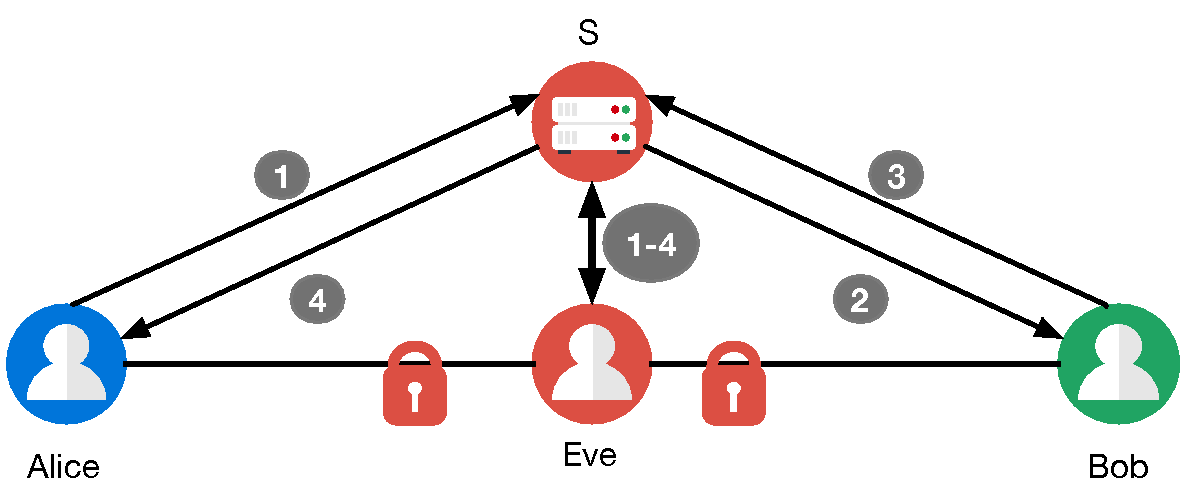
\includegraphics[width=.8\textwidth]{images/mitm}
\caption[WebRTC Man-in-the-Middle Attack]{WebRTC Man-in-the-Middle attack. The \gls{sdp} messages are: (1) Alice's offer relayed to Eve, (2) Eve's offer impersonating Alice, (3) Bob's anwser, (4) Eve's answer.}
\label{fig:mitm}
\end{figure}

To solve this issue, WebRTC proposes a mechanism for peers to authenticate to one another using an \gls{idp} as a trusted third party.
We refer to this mechanism as the WebRTC identity architecture, presented in Figure~\ref{fig:webrtcDeployId}.
To authenticate, peers bind their session fingerprint to a human readable identity by providing an identity assertion.
This identity assertion covers two main claims: the user identifier and the session fingerprint used.
By verifying the assertion and comparing it to the received session fingerprint attribute, peers can authenticate the other peer and verify that no man-in-the-middle attack is being mounted.

\begin{figure*}
\centering
\begin{subfigure}{\textwidth}
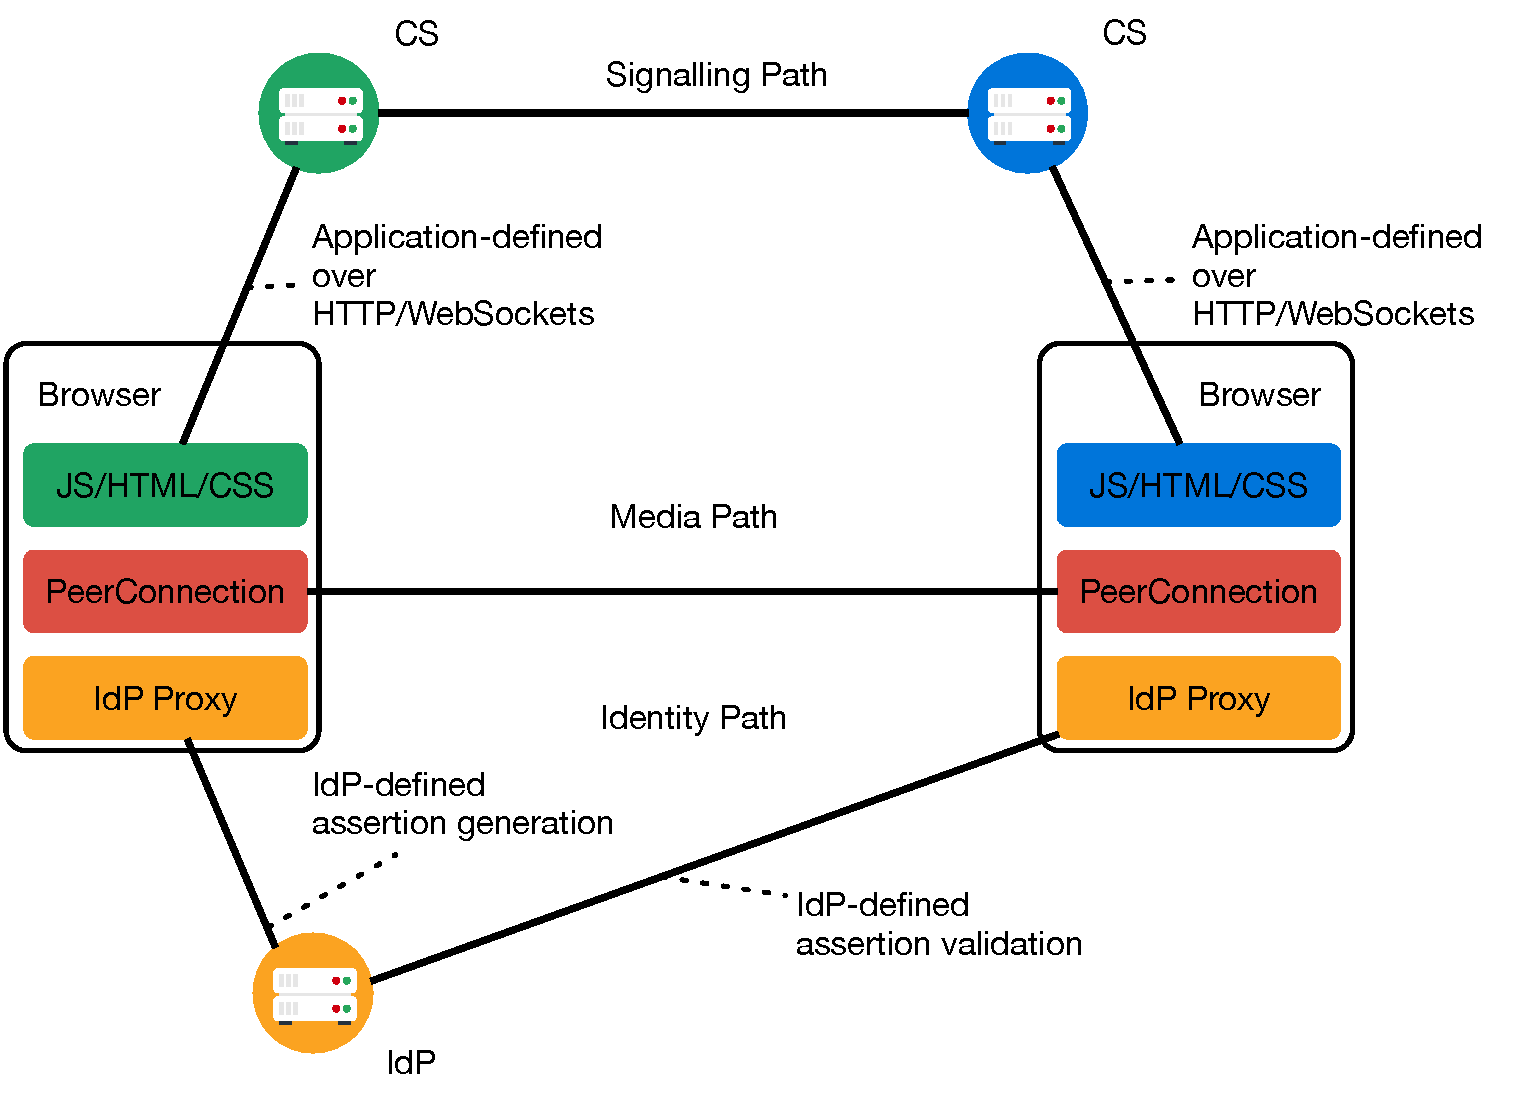
\includegraphics[width=.9\textwidth]{images/webrtcDeploymentId}
\caption[WebRTC deployment with two browser endpoints]{WebRTC deployment with two browser endpoints, two signalling servers, and a single identity provider authenticating the left-side peer.}
\label{fig:webrtcDeployId}
\end{subfigure}
~
\begin{subfigure}{\marginparwidth}
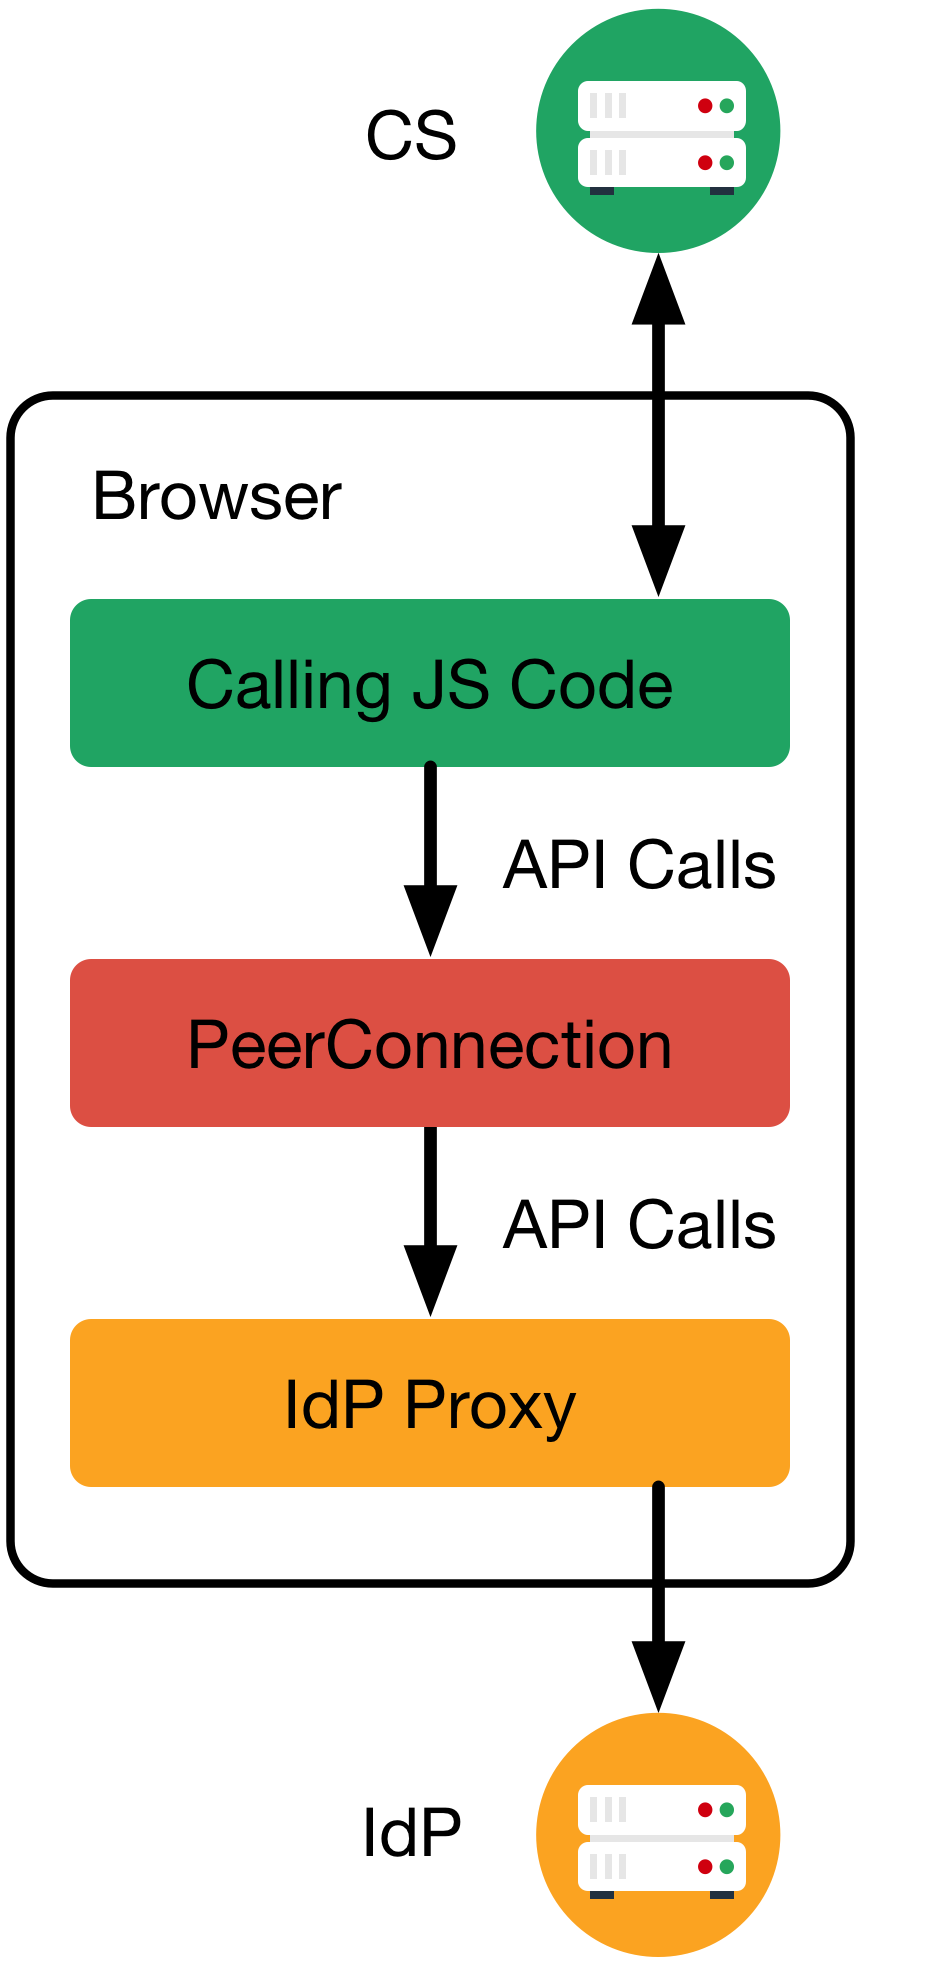
\includegraphics[width=\marginparwidth]{images/webrtcIdPProxyArch}
\caption{WebRTC Identity API Architecture}
\label{fig:webrtarch}
\end{subfigure}
\caption{WebRTC Identity Architecture}
\end{figure*}

In order to enable the generation and the verification of identity assertions from any authentication delegation protocol and providers, the WebRTC security architecture~\cite{I-D.ietf-rtcweb-security-arch} specifies the \gls{idp} Proxy component.
This component serves as an interface between the WebRTC PeerConnection object and the \gls{idp} through the interface presented in Figure~\ref{idProxyWebIDL}.
The \gls{idp} Proxy is available at a well-known location on the \gls{idp} domain.
Before making an \gls{sdp} call offer or answer, the PeerConnection calls the \gls{idp} Proxy to generate an assertion covering the session fingerprint.
After the \gls{idp} authenticated the user, the identity assertion is returned.
This assertion is then included in the \gls{sdp} message in an \texttt{a=identity} attribute, along with the \gls{idp} Proxy location on the \gls{idp} domain.
This allows peers to discover \gls{idp} Proxy location without prior knowledge or relationship with the \gls{idp}.
On receiving an \gls{sdp} message containing an Identity Assertion, the PeerConnection object downloads the \gls{idp} Proxy from the specified location.
It then calls the \gls{idp} Proxy's assertion verification function.
If the verification is successful, the session fingerprint and the user identity are returned.

\begin{figure}[H]
\begin{Verbatim}[commandchars=\\\{\}]
dictionary \textcolor{matred}{RTCIdentityProvider} \{
    \textcolor{matred}{generateAssertion}(
        \textcolor{matblue}{DOMString}                    contents,
        \textcolor{matblue}{DOMString}                    origin,
        \textcolor{matred}{RTCIdentityProviderOptions}   options,
    ),
    \textcolor{matred}{validateAssertion}(
        \textcolor{matblue}{DOMString}                    assertion,
        \textcolor{matblue}{DOMString}                    origin,
    )
\end{Verbatim}
\caption{Interface Exposed by Identity Providers in WebIDL.}
\label{idProxyWebIDL}
\end{figure}

The WebRTC specification allows users to choose a default \gls{idp} in their browser preferences if none was specified by the \gls{cs}.
But implicitly, if the \gls{cs} sets up an \gls{idp} to authenticate a WebRTC call, we would expect it to be the same \gls{idp} used to sign into the \gls{cs}'s website.
Indeed, the \gls{cs} must be able to handle the authentication procedure and needs to know that the user has an active account on this \gls{idp}. 
Besides, from a user experience perspective, it is important that the identity presented on the \gls{cs} webpage and the one received in the identity assertion are consistent with each other.
In practice, the choice of \gls{idp} would thus be defined by the \gls{cs} and limited in the same way as for common authentication delegation services.
We refer to this constraint as \textit{identity continuity}.


\subsection{Considered Protocols for WebRTC Peer Authentication}
\label{sec:authProtocol}
In this section, we present the authentication delegation protocols considered for integration with the WebRTC identity architecture~\cite{I-D.ietf-rtcweb-security-arch}.
These protocols are the BrowserID - Mozilla Persona protocol and the OAuth~2 protocol and its identity extension OIDC.
Figure~\ref{idmstandards} replace these protocols in the history of standards and technologies for user identity management.
As it is a technical prerequisite to both protocols, we first explain the JSON Web Token standard.  

\begin{figure*}
\centering
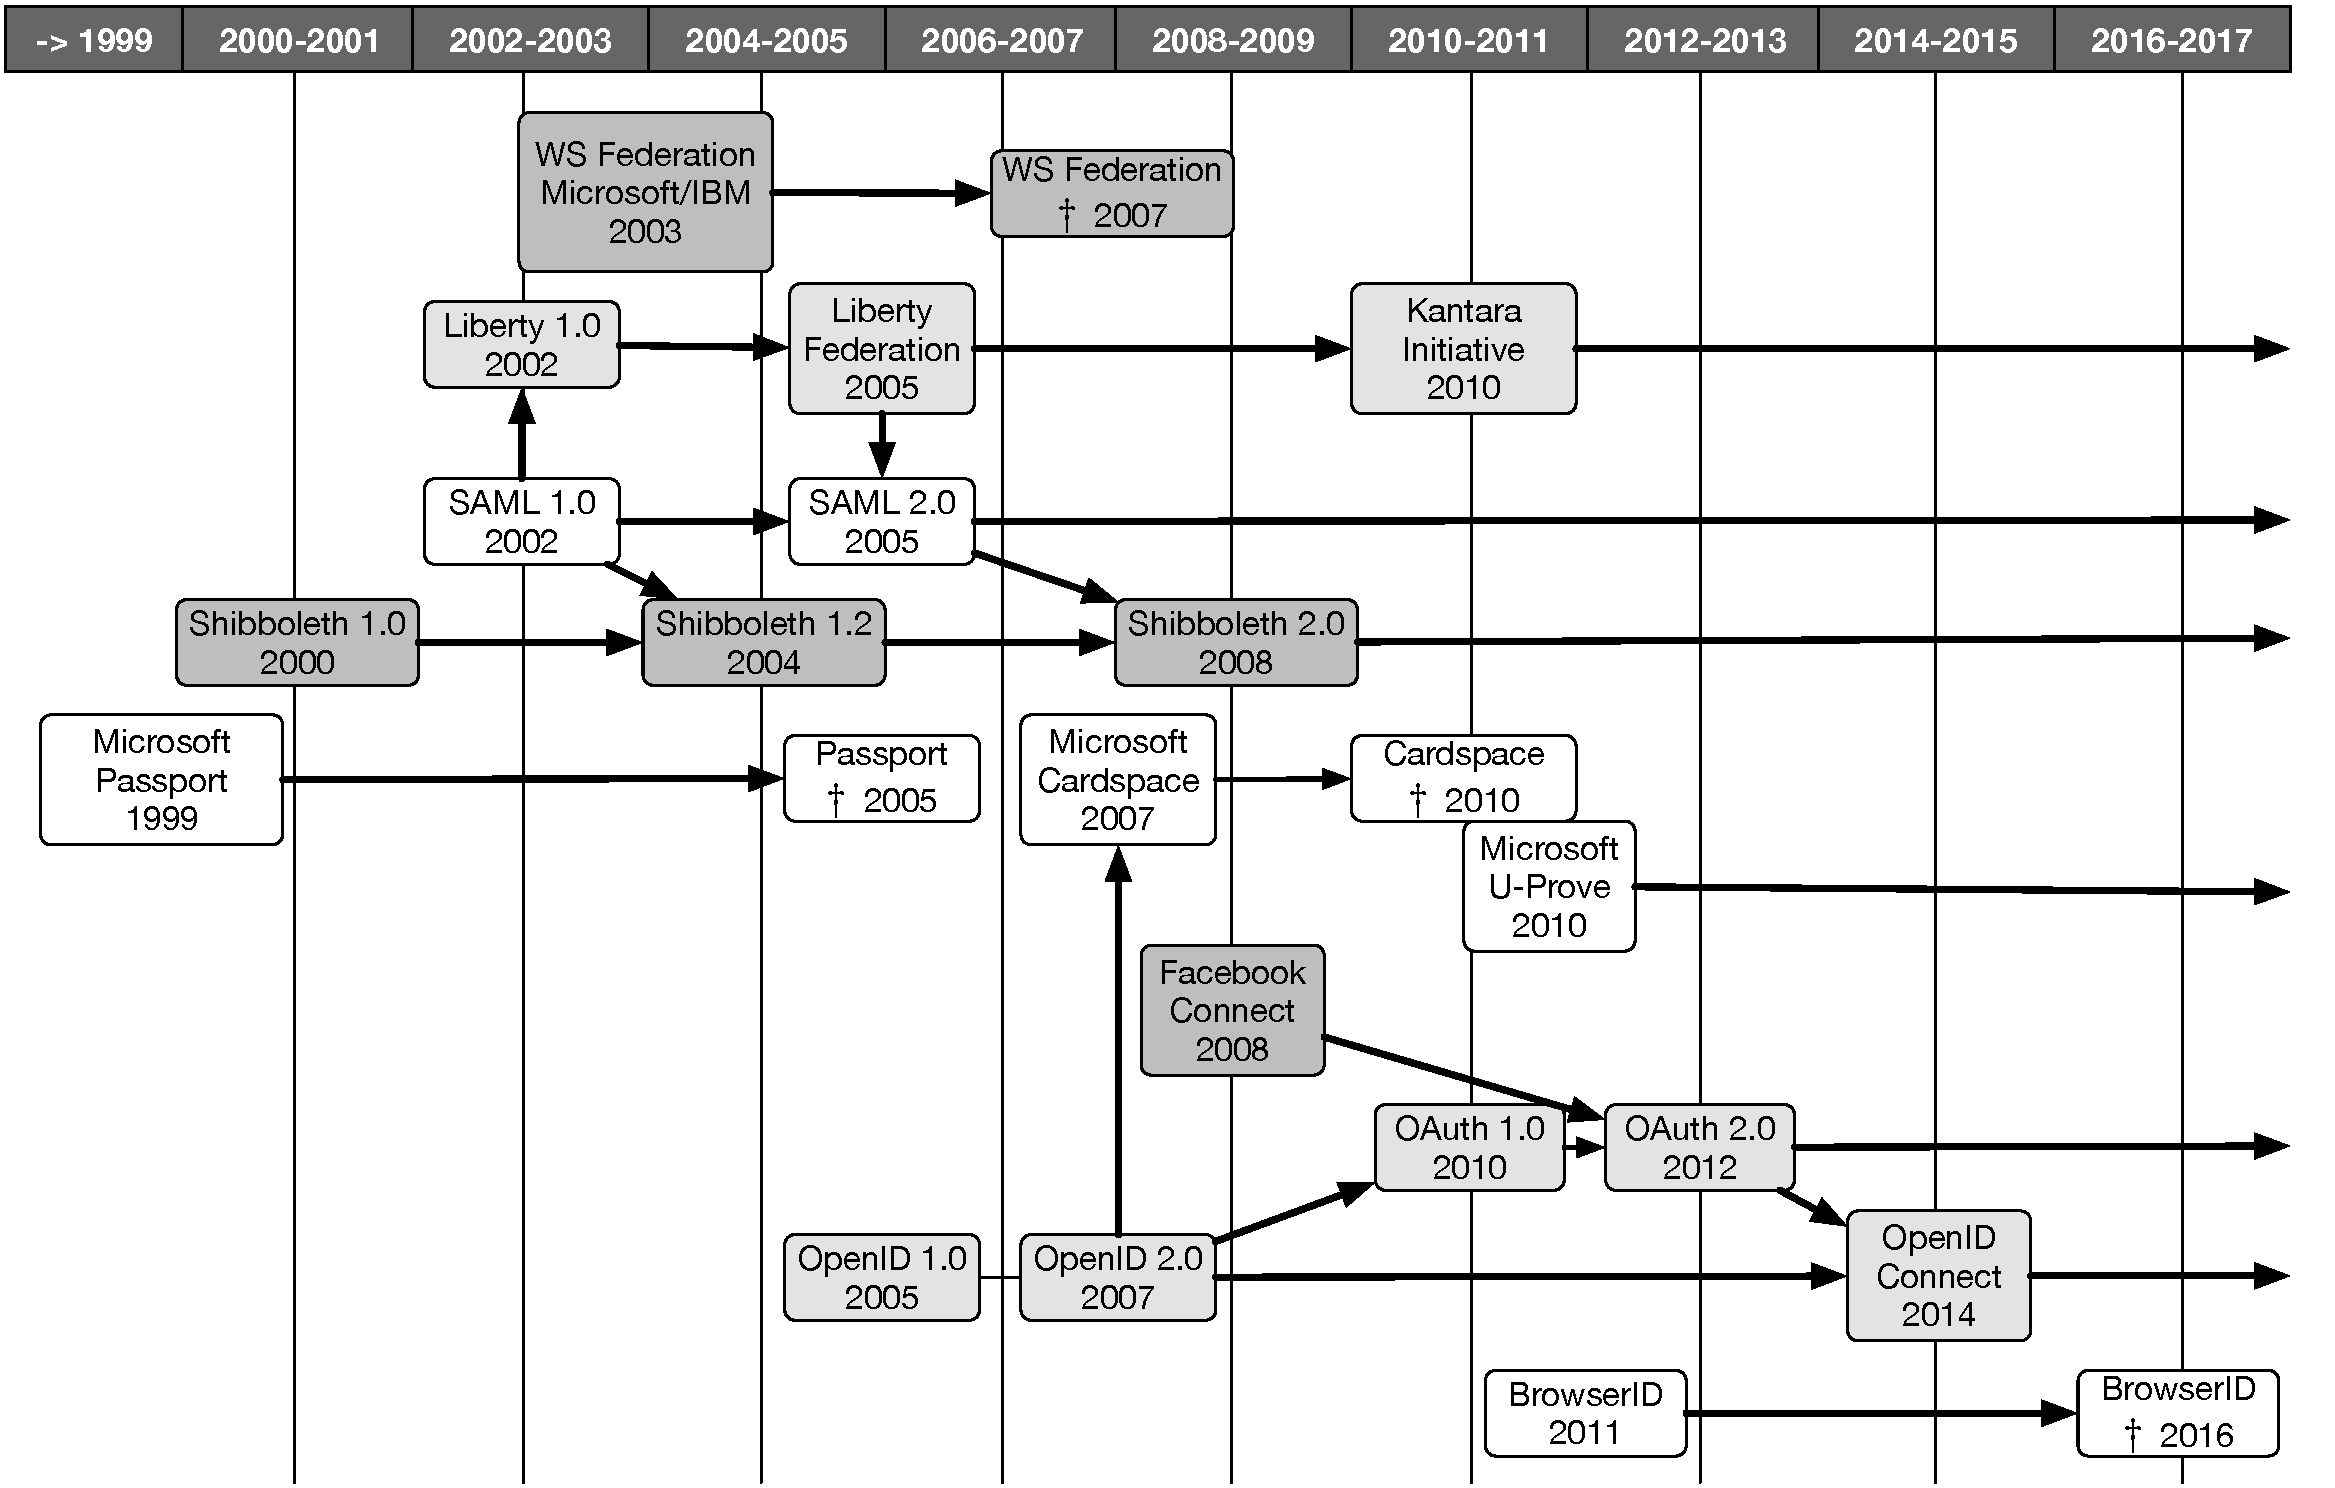
\includegraphics[width=\overflowingheadlen]{images/idmstandards}
\caption{Evolution of standards and technologies for user identity management, updated from J{\o}sang's 2014 survey~\cite{josang14}.}
\label{idmstandards}
\end{figure*}

\subsubsection{JSON Web Token}
\label{jwt}
\gls{jwt}, specified by \gls{rfc}~7519~\cite{RFC7519}, is a way of representing claims to be exchanged by two parties.
These claims are encoded in a \gls{json}~\cite{RFC7159} object which can then be signed as a \gls{jws}~\cite{RFC7515} or encrypted as a \gls{jwe},~\cite{RFC7516}.
\gls{jws} and \gls{jwe} tokens contain several \gls{json} members and in particular, a header and a payload or cyphertext, \ie the \gls{jwt} claims set.
These tokens can be compactly serialised by concatenating their base~64 encoded members.
The acronym \gls{jwt} is commonly used in place of \gls{jws} or \gls{jwe} depending on the context.

For instance, the following set of claims describes the subject \texttt{248289761001} whose name is \texttt{Jane Doe}.
The token was issued by \texttt{http://server.example.com} at \texttt{1509105796} seconds since the \gls{posix} Epoch, \ie January the 1st of 1970.

\begin{verbatim}
{
  "iss": "http://server.example.com",
  "sub": "248289761001",
  "aud": "s6BhdRkqt3",
  "nonce": "n-0S6_WzA2Mj",
  "exp": 1509192196,
  "iat": 1509105796,
  "name": "Jane Doe",
  "given_name": "Jane",
  "family_name": "Doe",
  "gender": "female",
  "birthdate": "1987-01-01",
  "email": "janedoe@example.com",
  "picture": "http://example.com/janedoe/me.jpg"
}
\end{verbatim}

The following \gls{jose} header describes the usage of the \texttt{RS256} algorithm and the key with id \texttt{1e9gdk7}.
RS256 is the compact representation of the \texttt{RSASSA-PKCS-v1\_5 using SHA-256} algorithm, \ie a public key signature algorithm.

\begin{verbatim}
{"kid":"1e9gdk7","alg":"RS256"}
\end{verbatim}

Serialisation of this token is done by encoding both components in base~64 and concatenating them separated by a dot.
The signature is then computed by using this string and the specified algorithm and appended to the serialised token.
The following text is the previous \gls{jwt} and \gls{jose} header examples signed into a \gls{jws}. 
The red part is the header, the violet is the \gls{jwt} payload, and in blue is the signature~\footnote{}.

\begin{figure}[H]
\begin{Verbatim}[commandchars=\\\{\}]
    \textcolor{matred}{eyJraWQiOiIxZTlnZGs3IiwiYWxnIjoiUlMyNTYifQ}.\textcolor{matviolet}{eyJpc3MiOiJodHRwOi}
    \textcolor{matviolet}{8vc2VydmVyLmV4YW1wbGUuY29tIiwic3ViIjoiMjQ4Mjg5NzYxMDAxIiwiYXV}
    \textcolor{matviolet}{kIjoiczZCaGRSa3F0MyIsIm5vbmNlIjoibi0wUzZfV3pBMk1qIiwiZXhwIjox}
    \textcolor{matviolet}{NTA5MTkyMTk2LCJpYXQiOjE1MDkxMDU3OTYsIm5hbWUiOiJKYW5lIERvZSIsI}
    \textcolor{matviolet}{mdpdmVuX25hbWUiOiJKYW5lIiwiZmFtaWx5X25hbWUiOiJEb2UiLCJnZW5kZX}
    \textcolor{matviolet}{IiOiJmZW1hbGUiLCJiaXJ0aGRhdGUiOiIxOTg3LTAxLTAxIiwiZW1haWwiOiJ}
    \textcolor{matviolet}{qYW5lZG9lQGV4YW1wbGUuY29tIiwicGljdHVyZSI6Imh0dHA6Ly9leGFtcGxl}
    \textcolor{matviolet}{LmNvbS9qYW5lZG9lL21lLmpwZyJ9}.\textcolor{matblue}{iYiil5mBuznlG5aGMnOeHkVALg41q1aK}
    \textcolor{matblue}{BFCoXW2f5sth3mZtkCwaRWUbj18pMN7iXlJOOdp9YVthccXORflV1hHlMKnrI}
    \textcolor{matblue}{aqlsoTo6aSnAHVgCJc64pKKMTOsIF0EVhcJ-obigxx0UOvme8AV1oQQkn8Bzc}
    \textcolor{matblue}{2Dd9E5D0qJX5YbeDw}
\end{Verbatim}
\caption[A JWT Example: OIDC ID~Token]{A JWT Example: OIDC ID~Token. Visit \url{https://jwt.io} to decode the token. It can also be verified using the following public key: 

\footnotesize{\texttt{-{}-{}-{}-{}-BEGIN PUBLIC KEY-{}-{}-{}-{}-
MIGfMA0GCSqGSIb3DQEBAQUAA4
GNADCBiQKBgQCrpVE2fAdanHGf
HA10RkmNPIFvCry5XMccRguIGR
zU9wgVBfJ+UeChN9GmcmGf67bE
GbtOY7mScWidKpm3u+XZUOXfl3
PQTF3kIPzKU2cOUwDeziHRmGKR
QXvtTy2esBH45GKzKjFHH6ti6o
Uy3QG7wSZ7kXGGS6pgXjkPBU6y
qwIDAQAB\\
-{}-{}-{}-{}-END PUBLIC KEY-{}-{}-{}-{}-}}}
\label{fig:jwt}
\end{figure}

\subsubsection{BrowserID - Mozilla Personna}
\label{sec:browserid}
BrowserID~\cite{browserid-specs} was Mozilla's attempt at a decentralized \gls{sso} protocol. 
Though it has been deprecated in 2016 due to a declining usage, the protocol was a central example of the WebRTC identity architecture~\cite{I-D.ietf-rtcweb-security-arch} interoperability claim.
Mozilla Persona was the BrowserID service hosted by Mozilla and using a simple email ownership verification mechanism to authenticate users.
The reason for the failure of BrowserID is probably that it did not attract enough interest from potential \gls{idp}.

BrowserID adds the \textit{id} property to the browser's \textit{window.navigator} object.
This property exposes several functions allowing a website client script to request an identity assertion from the browser.
The browser responds to identity assertion requests with a signed \gls{jwt}.
This \gls{jwt} contains the user identifier and a certificate for the user's public key corresponding to the \gls{jwt}'s signature.
The \gls{idp}'s public key verifying the certificate is publicly exposed on the \gls{idp}. 
Any website can verify the certificate's signature thus establishing a trust chain from the user to the \gls{idp}.

The BrowserID protocol allows any domain to be used as an \gls{idp} by signing a certificate for the user.
The user identifier must be an email address whose domain corresponds to the \gls{idp}'s domain name.
The email's domain allows \gls{idp} discovery as the location of the \gls{idp}'s public key and other endpoints are standardised on a \texttt{/.well-known} route.
The browser stores user's certificates and is then responsible for signing identity assertion for requesting website.
This separation of functionalities between the \gls{idp} and the browser allows for a privacy-friendly approach as the \gls{idp} is not aware of which site is the user login into.

Hiding the user's login actions behind a trusted component is also an approach proposed by Orange with the Trusted Identity Module~\cite{tim}.
Similarly, our technique described in the patent for a Method of managing the authentication of a client in a computing system~\cite{corre_authent} protects user privacy by putting the identity assertion in a decentralised network such as a blockchain.
In these architectures, the \gls{idp} cannot monitor who is verifying the identity assertion.


\subsubsection{OAuth 2 and OIDC}
\label{sec:oauth2}
\label{sec:oidc}

\begin{figure}
\begin{subfigure}{.3\textwidth}
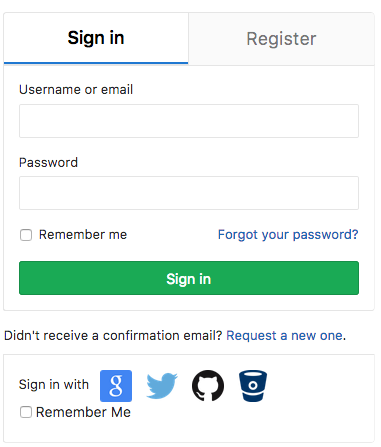
\includegraphics[width=\marginparwidth]{images/signinGitlab}
\caption[Sign in page]{GitLab sign in page with a selection of IdP.}
\label{fig:signinGitlab}
\end{subfigure}
~
\begin{subfigure}{.3\textwidth}
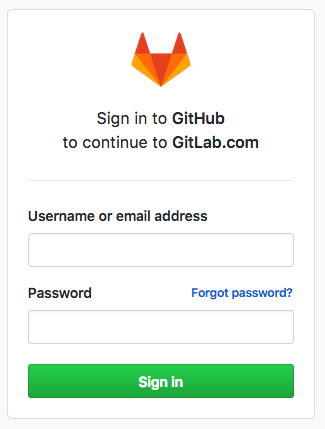
\includegraphics[width=\marginparwidth]{images/authnGitlab}
\caption[Redirection page]{Redirection to Github sign in page for Gitlab.}
\label{fig:authnGitlab}
\end{subfigure}
~
\begin{subfigure}{.3\textwidth}
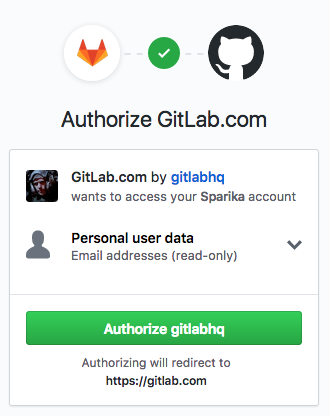
\includegraphics[width=\marginparwidth]{images/authzGitlab}
\caption[Consent page]{Github consent page to share email with Github.}
\label{fig:authzGitlab}
\end{subfigure}

\caption[OAuth~2 Process Example]{OAuth~2 process involving Github as AS and RS, and Gitlab as client.}
\label{fig:oauth2Gitlab}
\end{figure}

With more and more content being published by users, websites and in particular social networks need a way to securely expose their \gls{api}.
In order to respect users' privacy, it is, however, necessary to get users' consent to share private information. 
The original OAuth specification was published in 2006 as a solution to the problem of authorization delegation.
OAuth was then standardised by RFC~5849~\cite{RFC5849} and later deprecated by RFC~6749~\cite{RFC6749}: the OAuth~2.0 protocol.

The OAuth~2 specification defines four roles.
The \gls{ro}, in most case a user, is legally capable of granting access to the resource.
The \gls{rs} is where the resource is hosted.
The Client is the application requiring access to the resource on behalf of the resource owner and with its authorization.
Finally, the \gls{as} can grant an access token to the client after getting the resource owner consent.

The main OAuth~2 protocol flow is called the code flow, represented in Figure~\ref{fig:oauthsequence}.
Figure~\ref{fig:oauth2Gitlab} shows the user actions in such a flow.
An OAuth~2 flow is based on \gls{http} and make use of redirection response (code 300) to let servers exchange information on behalf of the user.
In this flow, the client makes an \gls{http} request for an authorization from the \gls{ro} for a specific resource (1 in Figure~\ref{fig:oauthsequence}).
The \gls{as} authenticates the user (Figure~\ref{fig:authnGitlab}) and then asks for his consent (Figure~\ref{fig:authzGitlab}).
The requested authorizations are transmitted to the \gls{as} in the \textit{scope} parameter of the \gls{http} authorization request.
After the \gls{as} got the user's consent, the request is redirected to the client (2).
This redirection contains an authorization code, for instance in the URL query parameter, which can be retrieved by the client.
The client then exchanges the authorization code with the \gls{as} for an access token (3, 4).
This exchange happens out of the \gls{ro} scope and allows the \gls{as} to authenticate the client.
The access token is then used to access the resource on the \gls{rs} (5,6).
In order to be authenticated by the \gls{as}, the client must be registered.
The process of registration most often involves the client's developer taking manual actions to register on the \gls{as} through HTML forms.
However, automatic discovery and registration are also possible if the \gls{as} exposes some metadata and registration endpoints.
%Although specifications for automatic discovery and registration exist for both OAuth~2 and OpenID Connect, we show in \ref{OAuth study} that they are not implemented by AS.

\begin{figure}
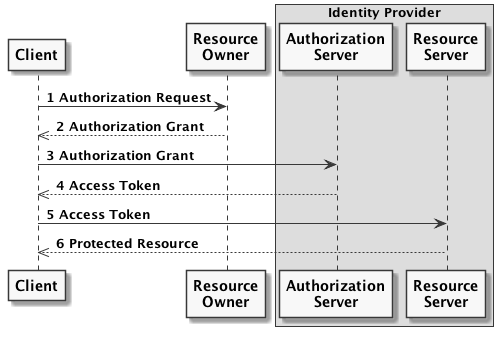
\includegraphics[width=.78\textwidth]{images/oauth2}
\caption{Abstract Oauth~2 code flow taken from RFC~6749.}
\label{fig:oauthsequence}
\end{figure}

In the alternative implicit flow, the \gls{as} directly responds to the authorization request with the access token rather than with an authorization code. 
This simplified flow is adapted for client implemented in the browser rather than on a server.
In such scenario, the client code is visible from the user and cannot protect a secret key. 
As a result, the client cannot be authenticated by the \gls{as} and the authenticated authorization grant is unnecessary.
However, the resulting process is less secure as the access token may be exposed on the web browser.

While OAuth~2 is able to convey user authentication information, it does so in non-standard ways left for implementors to decide.
Actually, authentication in OAuth~2 is implicit as it is assumed that the user was authenticated by the \gls{as} in order to get the user's consent.
For the client, getting the user's email means that the owner of the email has been authenticated, but it does not know much more than that.

\glsreset{oidc}
\gls{oidc}, developed by the OpenID foundation, is ``a simple identity layer on top of the OAuth 2.0 protocol''~\cite{sakimura_openid_2014}.
It allows clients to retrieves an ID~Token in parallel from the access token.
This ID~Token is a \gls{jwt}, containing information related to the user's identity, as the one in Figure~\ref{fig:jwt}.
In addition to the ID~Token and additions to the OAuth~2 protocol, OIDC standardises a set of identity claims.
A client using OpenID Connect and requesting an ID~Token must add the \textit{openid} scope to his OAuth~2 authorization request.
The received ID~Token contains a list of attributes describing the user's authentication result.
In particular, the triple of identifiers \textit{iss}, \textit{sub}, \textit{aud} respectively identify the token ISSuer (\ie the \gls{as}), the SUBject (\ie the user), and the token AUDience (\ie the client).
The audience identifier certifies to the client that it is the intended audience of the token and is not subject to replay attacks.
Note that to avoid correlation attacks (as described in Section~\ref{sec:privacy}), the subject identifier must be locally unique \ie the same user must not have the same \texttt{sub} identifier for two different clients.
The ID~Token also contains expiration time and security parameters such as authentication time, nonce, and authentication level.
The requested claims describing the user identity can either be contained in the ID~Token or retrieved from the UserInfo endpoint.
This endpoint is an OAuth~2 protected resource that can be accessed with a valid access token for the \texttt{openid} scope.
While \gls{oidc} standardises a set of identity claims, additional claims can be added freely to both the ID~Token and the UserInfo endpoint as long as they use collision-resistant names or that naming conflicts are unlikely.

From a user's point of view, the difference between OAuth~2 and \gls{oidc} flows should not be visible.

\subsection{Alternative Key Management Protocols}
\label{sec:keymanagement}
\gls{dtlssrtp} and \gls{dtls} in conjunction with the use of the identity path allow to bind negotiated keys to an identity authenticated by an \gls{idp}.
Although these are the default and preferred key management protocols respectively for media and data channels, alternative key management protocols offer different security guarantees.
In this section, we present the SDES and ZRTP protocols.

The \gls{sdes}~\cite{RFC4568} was the main competitor to \gls{dtlssrtp} as the default security protocol for WebRTC.
The main advantage of \gls{sdes} consists in its existing deployment in existing \gls{sip}/\gls{rtp}~\cite{I-D.ohlsson-rtcweb-sdes-support} based \gls{voip} networks\footnote{VoIP designates the techniques to communicate using voice or voice and video over any compatible \gls{ip} networks.}.
In particular, interconnectivity between WebRTC and \gls{sip}/\gls{rtp} endpoints would require the deployment of media gateways.
As media gateways are complex and costly to implement, leveraging the existing implementations of \gls{sdes} gateways would reduce costs and favour WebRTC interconnectivity.
Additionally, due to the existing \gls{sdes} deployment, gateways may not have to decrypt/encrypt session negotiated with \gls{sdes} thus achieving end-to-end encryption.
However, contrary to \gls{dtls}, in the \gls{sdes} protocol keys are exchanged in clear over the signalling path inside \gls{sdp} messages.
This implies that the \gls{cs} can decrypt the streams invisibly.
While this seems to be a major vulnerability, in the context of real-time communication it may be a legit requirement from \gls{cs} as they may be subject to lawful interception requirements.
In comparison, mounting lawful intercept against \gls{dtlssrtp} is mainly possible through a \gls{mitm} interception as described earlier\footnote{Note that in interconnectivity scenarios, gateways can decrypt \gls{dtlssrtp} streams unless both endpoints are using \gls{dtlssrtp} in conjunction with verified identity assertions.}.
\gls{dtls} was considered by the \gls{ietf} as offering stronger security guarantees and qualified as mandatory to implement.
Furthermore the implementation of both the \gls{dtls} and \gls{sdes} protocols may allow for a downgrade attack.
To implement such attack, a malicious service would have to modify the \gls{sdp} messages to only advertise \gls{sdes} support.
As a result, peers could negotiate a lower security level, allowing the service to then mounts an invisible interception attack. 
Not only was \gls{dtlssrtp} preferred over \gls{sdes}, but \gls{sdes} was also not authorized for implementation in WebRTC endpoints.

\marginpar{
\captionsetup{type=figure}
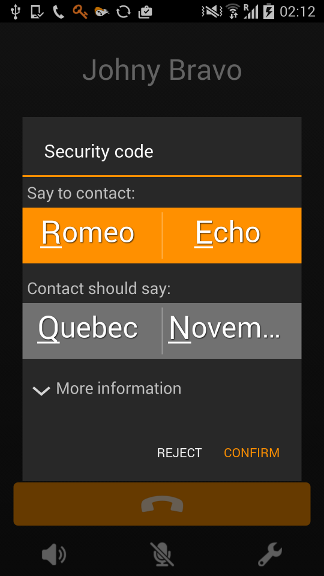
\includegraphics[width=\marginparwidth]{images/zrtp}
\caption{Phone-X application displaying the ZRTP SAS.}
\label{fig:zrtp}
}

The ZRTP protocol~\cite{RFC6189} is a media path keying protocol for \gls{srtp}.
It uses a simple Diffie-Hellman exchange to agree on the symmetric session key.
A \gls{sas} is then derived from the session-key and vocally transmitted over the media path (see Figure~\ref{fig:zrtp}).
As both peers compare the exchanged \gls{sas}, \ie $hash(K_A) = hash(K_B)$, they get a confirmation that they negotiated the same session-key and that no MitM is being set up, \ie $K_A = K_B$. 
Although the \gls{sas} comparison is vulnerable to a real-time audio spoofing attack, in practice it is quite complicated.
Indeed, to succeed and remain undetected, the attacker must inject his own \gls{sas} at the right moment.
This requires detecting, how, when, and which one of the peers will say the \gls{sas}.
Video session may further deter such attack.
However, practical attacks and bugs on ZRTP implementations have been recently reported~\cite{SchurmannKHW17}.
As a matter of fact, ZRTP is currently implemented by multiple \gls{voip} clients offering end-to-end encryption.
But their reliance on the \gls{sas} vocal comparison procedure and their implementations of different security indicators and procedures may be confusing for most users.
ZRTP is also less flexible than the \gls{idp} Proxy solutions of WebRTC as it is only adapted for the \gls{voip} use case.
WebRTC data channels, uni-directional communications, or non-human peer use cases cannot be secured by ZRTP.









%%%%%%%%%%%%%%%%%%%%%%%%%%%%%%%%%%%%%%%%%%%%%%%%%%%%%%
%%%%%%        TRUST
%%%%%%%%%%%%%%%%%%%%%%%%%%%%%%%%%%%%%%%%%%%%%%%%%%%%%%

\section{Trust}
\label{sec:trustintro}
Evaluating the security of a system is only possible if it can be observed and monitored.
In communication scenarios, only a fragment of the whole system is under the user control.
The rest of the system is controlled by other peers, certificate authorities, communication service providers, identity providers, and public internet service providers or enterprise network administrators.
If a complete monitoring is not possible, it may be necessary to make a trust decision.
In this section, we define trust and the properties often associated with formal trust models.
We then explain the actual WebRTC trust model.

\subsection{Introduction on Trust}
Experienced every day, trust is nonetheless hard to define due to the broad range of situations and interactions it covers. 
Several definitions of trust have been proposed.
Inspired by McKnight and Chervany~\cite{mcknight1996meanings}, J{\o}sang and Presti define trust as: ``\textbf{the extent to which one party is willing to depend on something or somebody in a given situation with a feeling of relative security, even though negative consequences are possible}''~\cite{josang2004analysing}.
In the sense of an action, we would say that trust is the decision of intelligent agents to cooperate in the face of risk and uncertainty about the behaviour (capability or intention) of other agents.
This heuristic is often based on prior interaction history, reputation from a community, or recommendations from other trusted sources.

A truster is a person, an organisation, or a software agent while a trustee is an agent, possibly non-intelligent, that can provide a service to the truster.
Figure \ref{fig_trust} presents such a simple trust relationship.
Trust between two agents is asymmetric and depends on a specific context, \ie a specific scope of action for which trust is granted. 
Transitivity is a property commonly associated with trust relationship where an agent D would recommend its trust in E to B (see Figure~\ref{fig_trustnet}).
As capability in a given context does not imply the capability to recommend other agents in the same field of expertise, transitivity is not present in all models.
However, a recommendation could be seen as a context allowing transitivity to other contexts.
Indeed, J{\o}sang and Pope describe a transitive path as a chain of recommending trust terminated by a functional trust~\cite{josang2005semantic}. 
Trust recommendation can also be aggregated from multiple sources.
Figure~\ref{fig_trustnet} shows trust transitivity and aggregation. 
Dashed arrows represent recommendations, while the dotted arrow represents the trust relation from A to E built from recommendations aggregation. 


\marginpar{
\centering

\captionsetup{type=figure}
\caption{Trust representation}
\label{fig_trust2}

\captionsetup{type=subfigure}
\begin{tikzpicture}[transform shape, scale=.8]
\node(A)[circle, fill=gray!30] at (0,0) {Truster};
\node(B)[circle, fill=gray!30] at  +(3,0) {Trustee};
\node(T) at  +(1.5,0.5) {Trust};
\draw [->][thick] (A) -- (B);
\end{tikzpicture}
\caption{Trust relationship}
\label{fig_trust}
\bigskip

\captionsetup{type=subfigure}
\begin{tikzpicture}[transform shape]
\tikzstyle{every node} = [circle, fill=gray!30]
\node(A) at (0,6) {A};
\node(B) at  +(.5,4) {B};
\node(C) at  +(-.5,4) {C};
\node(D) at  +(0,2) {D};
\node(E) at  +(0,0) {E};
\foreach \from/\to in {D/E}
\draw [->][thick] (\from) -- (\to);
\foreach \from/\to in {A/B, A/C, B/D, C/D}
\draw [->][dashed] (\from) -- (\to);

\draw [->][dotted, thick] (A) to [out=-45,in=45] (E);

\end{tikzpicture}
\caption{Trust transitivity}
\label{fig_trustnet}
\medskip

}

Methods to establish trust are commonly categorised between policies and reputation based~\cite{artz2007survey}:
\begin{itemize}
\item Policies describe the ``hard evidence'' requirements to obtain trust in a situation where trust in an agent itself is unknown but there is an existing trust in a third party authority. 
\item The concept of reputation describes the perception of a community on the reliability of an agent part of this community for a particular context.
%An opinion is a subjective view of an agent about another agent's past behaviour. 
%Reputation in a community is thus formed by the aggregation of opinions by means of recommendation. 
These recommender systems are either organised by a trusted third party or in a peer-to-peer fashion.
Furthermore, recommender systems can only establish a reputation in a network where data about agents' behaviour is available.
\end{itemize}

Trust relationships are dynamic as new feedback and credentials creation or revocation will impact previously existing trust. In some models, recommendations are part of this dynamic as delay can occur in a trust information propagation.
Time may also play an important role in trust dynamic, either as an ageing factor determining ponderation of new experience over previous ones or as an eroding factor decreasing trust or the precision of a trust value. 

Various trust metrics have been proposed ranging from discrete or fuzzy to continuous scale~\cite{artz2007survey}.
We observe two categories of trust measure representations that differ from their representation of distrust. 
The first category represents trust on a scale of $[-x;+x]$ with the negative value representing distrust, and zero a neutral trust.
The second category uses a scale of $[0;x]$ with 0 representing full distrust.
In the first case, a bad recommendation by a distrusted source contributes positively to the final trust level, while on the second computational model, the recommendation would simply be discarded due to a low ponderation.
Other representations can be considered as a special case of these two categories.

Authors in the literature~\cite{mui2002computational,josang2006exploring} define operators for trust relationships. In these models, trust transitivity is generally computed with a multiplicative operator while trust sources aggregation is modelled by an averaging operator. Some models may as well represent certainty and distrust. These models handle contradiction in trust recommendation and uncertainty of trust sources. 

\subsection{The WebRTC Trust Model}
From a security perspective, trust is often synonym with ``providing proofs of identity, authorization, and performance''~\cite{artz2007survey}.
Although multiple formal trust models have been proposed and refined in the literature~\cite{artz2007survey}, commercial softwares and services often make use of trust models in a simpler manner.
The current WebRTC trust model is an informal model categorising entities into three categories: the \gls{tcb}, authenticated entities, and unauthenticated entities.

At the root of the model is the WebRTC agent, in most cases a browser, which serves as the \gls{tcb}.
All security properties must be guaranteed by the \gls{tcb}, as we explained in Section~\ref{sec:tcb}.
In particular, the \gls{tcb} is responsible for authenticating other entities acting on the communication.

In WebRTC, authenticated entities are either \gls{cs}, \gls{idp} or other peers.
Optimally, these are cryptographically authenticated by presenting certificates via \gls{https} for servers, and \gls{dtls} or identity assertion for peers.
We previously described in Section~\ref{sec:pubkey} how \gls{ca} build a chain of trust from a root certificate to the final owner's certificate.
The trust chain is then anchored in the browser as it is browser makers who configure the list of root certificates in browsers.
Similarly, the signalling path forms a transitive recommendation path for media session security certificates.
Note that while these entities are authenticated, these may not necessarily be trusted\footnote{``Just because we can verify that https://www.evil.org/ is owned by Dr Evil does not mean that we can trust Dr Evil to access our camera and microphone''~\cite{I-D.ietf-rtcweb-security-arch}.}.
However, it is mandatory to authenticate entities before making a trust decision.
This trust decision is ultimately left for the user to decide.

In particular, while the \gls{cs} has a large control over the WebRTC session, in some scenarios it may be untrusted.
For this reason, the specification introduces an alternative identity path to exchange identity assertions.
These assertions bind media session security certificates to an identity and from a trust perspective, this forms an alternative transitive recommendation path.
Paradoxically, this identity path is left for the \gls{cs} to configure and control as it is the \gls{cs} who sets the \gls{idp} to use.
From our point of view, it is not clear if the identity path can be trusted independently of the \gls{cs}.
%This question underlies RQ3: \textit{Can we let users chose actors they trust to participate in the communication setup?}.

Other network elements are generally not authenticated by the browser.
The WebRTC specification thus assumes that they behave maliciously and the system is supposed to be secure against attacks from these entities.








%%%%%%%%%%%%%%%%%%%%%%%%%%%%%%%%%%%%%%%%%%%%%%%%%%%%%%
%%%%%%        PRIVACY
%%%%%%%%%%%%%%%%%%%%%%%%%%%%%%%%%%%%%%%%%%%%%%%%%%%%%%
\section{Privacy of the Call-Session}
\label{sec:privacy}
Some JavaScript web \gls{api} may expose critical data to malicious websites. 
To protect users these resources must be guarded against unwanted access.
This is done by enforcing explicit consent policies asking users whenever a website requests access to a sensitive \gls{api}.
Permissions may be granted or denied based and websites origin.
\gls{http} origins, considered insecure, are often limited to one time authorizations.
Considerations for privacy in internet standards is steadily increasing\footnote{The battery status \gls{api} was even removed after its implementation in browsers as its benefits were estimated less important than the privacy risk faced by users. This \gls{api} is now only available from privileged code in Firefox~\cite{batteryFF}.}.

\gls{rfc}~4949~\cite{RFC4949} defines privacy as ``the right of an entity (normally a person), acting on its own behalf, to determine the degree to which it will interact with its environment, including the degree to which the entity is willing to share his personal information with others''.
This definition emerged from the United States Privacy Act of 1974. which was concerned with the growing amount of personal data stored by the U.S. government.
In the meantime, the protection of personal data emerged in Sweden, France, and Deutschland, mainly driven by the fear of mass surveillance by an authoritarian state~\cite{usaeuprivacy}.
Privacy should not be used as a synonym for data confidentiality: as a right, privacy is a reason for security rather than a mean.
In this section, we describe types of privacy attack and possible mitigation techniques. 
We also give a brief overview of the legal regulation applying to personal data protection.
Finally, we present existing privacy considerations of the WebRTC security architecture.
%In the rest of the Context part, we will develop privacy consideration when necessary.
%In particular ... \todo{ref to privacy considerations in other context chapter and state of the art.}

\subsection{Attack and Threat Mitigation}
The risks associated with privacy threats are multiple~\cite{RFC6973}.
In the most trivial cases, individuals can suffer from the divulgation of their private life by financial or reputation loss.
Individuals can also feel a sense of unease by knowing or fearing the monitoring of their actions.
This feeling can even lead users to refrain from acting freely.
In the worst case, if the attacker is able to physically harm the individual, the individual's life may be endangered.
\gls{rfc}~6973~\cite{RFC6973} categorise privacy threats between combined security-privacy and privacy specific threats:
\begin{itemize}
\item \textbf{Combined security-privacy threats}
\begin{itemize}
\item Surveillance
\item Stored Data Compromise
\item Intrusion
\item Misattribution or Spoofing
\end{itemize}
\item \textbf{Privacy specific threats}
\begin{itemize}
\item Correlation
\item Identification
\item Secondary Use
\item Disclosure
\item Exclusion
\end{itemize}
\end{itemize}

Particularly related to the context of web real-time communications are the threats of surveillance, misattribution, correlation, and identification.
Surveillance is conducted by an attacker who observes or monitors the individual's communications.
The threat is present even if the communication is encrypted as the possibility of surveillance can lead the individual to change his behaviour, while the fact that the communication is happening may be enough knowledge for the attacker.
Misattribution of behaviour can happen as a result of inadequate or insecure authentication.
Similarly, a privacy attacker may also draw wrong conclusions based on his observations of the individual behaviour. 

Correlation threats are made possible by the combination of pieces of information regarding an individual.
By correlating pieces of information from different sources, an attacker may learn more than what the individual believes to have shared.
Finally, identification is the correlation of an individual's information in order to infer or establish the individual's identity.
For instance, browser fingerprinting techniques can uniquely identify a browser, and its associated user, by executing a set of JavaScript scripts on a website~\cite{laperdrix2016}.
Combined together these technical pieces of information can form a unique and portable identifier, without the user knowledge.

The main solution to mitigate privacy threat is data minimisation.
As it is difficult to define what information can cause a privacy risk, reducing data disclosure globally reduce the privacy attack surface.
Data minimisation is a general principle that should be applied by developers.
The most straightforward approach is to limit data collection to the minimum required, however, a limit may also be set to the time of retention of an information.
In some cases, individuals may themselves enforce data minimisation by reducing the information they expose to websites.
Though this may come as a tradeoff between privacy and functionalities.
If the original value of some data is legitimate, denying its usage can protect an individual's privacy but at a cost.
For instance, most browser fingerprinting techniques rely on the execution of JavaScript.
It is possible to deactivate JavaScript through browser's options but this would break most websites in the process.

An individual is said to be anonymous if it belongs to a set of individuals appearing to have the same attributes.
This set is called an anonymity set and individuals within it must be indistinguishable from each other. 
Anonymity is relative to the point of view of the attacker as it depends on the type of information the attacker can observe.
Additionally, the risk of correlation means that it may be difficult to assess if one belongs to an anonymity set or not.
A slight difference in attributes collected may de-anonymise an individual or at least reduce the size of the anonymity set.
Some privacy preserving approaches thus try to quantify the uniqueness of an attribute.

Respect for privacy recognises the right for an individual to determine to which degree it is willing to interact and share private information with its environment.
For this reason, data collection happening ``in secret'' can be detrimental to an individual's privacy. 
User participation approaches involve the individual in the collection process by asking his consent.
Though modern privacy regulations enforce a strict policy for explicit user consent (see Section~\ref{privacyRegulation}).
Depending on the use case and underlying architecture it may be easier or harder to explicitly ask the user for his consent.

Finally, security in itself is an essential component of privacy protection.
Confidentiality of exchanges and strong peer authentication ensure that data are protected against a malicious third party.

\subsection{Regulations}
\label{privacyRegulation}
Privacy-preserving regulations have been in development since the 1970's both in the USA and in European countries.
Growing concerns by citizens for their privacy on the Internet pushed legislators to adopt more protective legislation.
The new European \gls{gdpr}~\cite{gdpr} is a regulation adopted by the European Parliament in 2016 to reinforce and unify data protection for individuals within the \gls{eu}.

On one hand, the \gls{gdpr} simplify the regulatory environment by unifying it across the \gls{eu}.
On the other hand, the requirements for companies or public entities collecting personal data are more significant.
At the same time, possible sanctions are also more severe going up to 20 000 000 euros or 4\% of the global company revenue.
New principles are also introduced such as privacy by design and by default.
Privacy by design is a concept developed in 1995 by a joint-team from Canada and the Netherlands.
As defined by the \gls{gdpr} in its article 25, privacy by design means that appropriate technical and organisational measures should be taken both at design time and processing time.
The definition of Privacy by default states that appropriate measures should be taken to ensure that only necessary personal data are collected, processed, and stored for each specific purpose of processing.
This principle also comes with an obligation of conformity as soon as the design time of a personal data processing system.
The responsibility to implement and prove conformity regarding the regulation belongs to a Data Protection Officer appointed by each company or public entity.

Major differences oppose the United States and the \gls{eu} regarding how their laws protect the privacy of their citizens~\cite{usaeuprivacy}.
In the United States, privacy is a right recognised by the Constitution in order to protect citizens freedom from the government.
In addition, privacy-preserving laws are decided at the state level rather than at the federal level.
Oppositely, though the \gls{gdpr} also concerns public entities, the regulation is primarily aimed at the \gls{ott} companies often located in the United States. 
For users, the \gls{gdpr} introduces important new rights such as explicit consent, right to be forgotten, right of access, and right of rectification.
Furthermore, the \gls{gdpr} protects \gls{eu} citizens whether the company processing data is located inside or outside the \gls{eu}.
Such protective regulations from the \gls{eu} affect companies across the world forcing them to be compliant.
For these reasons, both United States and \gls{eu} laws are led to interact with each other.
In a similar fashion, several national legislation across the world have been influenced by European laws.

In the meantime, terrorist attacks are pushing governments to adopt new disposition to facilitate the collection and the exchange of data between security services.
While governments reinforce privacy preserving regulations and may invest in privacy-preserving research, communication surveillance is also an ever more important objective for their security services.
As an example of these contradictory efforts, the United States government is both funding research on the Tor network~\cite{DBLP:journals/popets/JohnsonJHSS17} and trying to break it through efforts of the National Security Agency~\cite{ball_nsa_2013}.


\subsection{Privacy Considerations for WebRTC}
The WebRTC security architecture intends to prevent several types of privacy attacks.
Persistent identifiers such as \gls{dtls} certificates allow for correlation attacks against anonymous call.
To prevent this, WebRTC implementations should allow resetting such identifiers, for instance with a similar lifetime as cookies or through a website-controlled mechanism.

\gls{ice} candidates addresses may also form a unique identifier, either by themselves or in conjunction with other web \gls{api} during browser fingerprinting attacks.
Alternatively, \gls{ice} candidates may be used to discover the peer's location.
Several mechanisms implemented by browsers allow controlling exposed candidates addresses.
For instance, users may deactivate the sharing of local candidates or force the use of a \gls{turn} relay.
The sharing of local candidates may also be bound to a consent mechanism, for instance when requesting \texttt{getUserMedia}~\cite{I-D.ietf-rtcweb-ip-handling}.
This trade-off between privacy and availability means that an optimal network path may not be available for the communication.


\subsection{Tor: Onion Routing}
\label{sec:tor}
Anonymity networks protect user's privacy from network surveillance and traffic analysis by anonymising their communications.
The most used anonymity network on the Internet is Tor\footnote{\url{torproject.org}}~\cite{INTA_DarkWeb}.
In this section we give an overview of Tor functioning, and explain how it is not practical for WebRTC.

Tor is an implementation of onion routing whose principle is to build an anonymous routing protocol on top of the Internet.
The goal of such protocol is to defeat traffic analysis attacks.
The Tor network is constituted of thousands of public routing nodes publishing their public key, and clients.
Clients often connect to Tor using Tor Browser, a privacy-preserving browser based on Firefox.


\marginpar{
\centering
\captionsetup{type=figure}
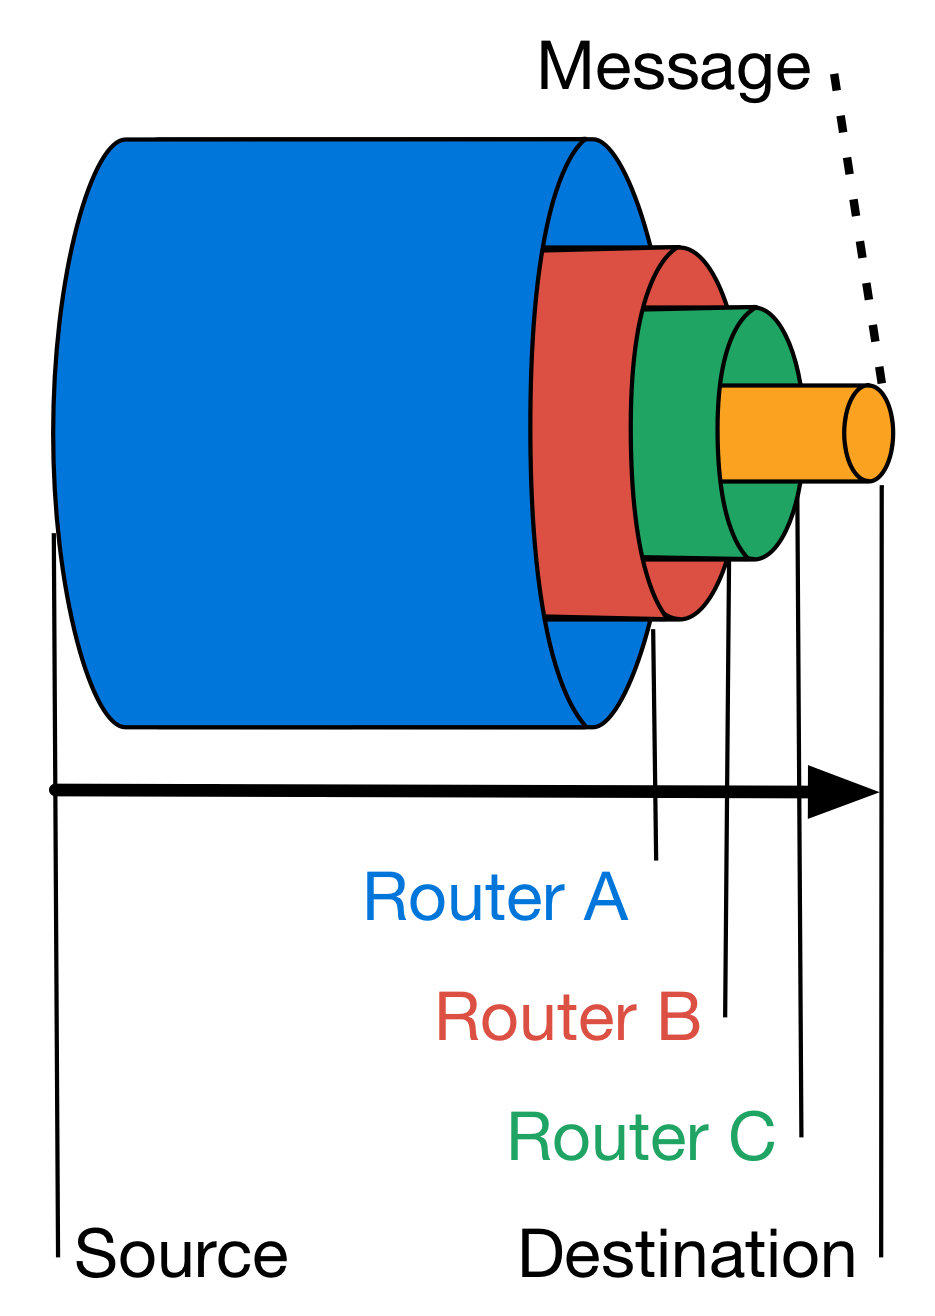
\includegraphics[width=\marginparwidth]{images/onion}
\caption[Tor Onion Encryption]{In this example, the message is sequentially encrypted with keys from router C, B, and A. It is then routed through these routers starting from A. Each router removes a layer of encryption and routes the message to the next router. Finally, router C transmits the message to the destination. This example is taken from \protect\url{wikipedia.org}.}
\label{fig:onion}
}

In order to establish a communication through Tor, a client randomly chooses nodes to build a routing circuit.
In a circuit, each node knows only the previous and next nodes.
The entry node (resp. the exit node) knows only the IP of the source client (resp. the destination client).
Before sending a packet to the circuit the client encrypts it sequentially with the public key of each nodes part of the circuit, starting from the exit node.
This creates layers of encryption around the original packet.
To route a Tor packet, each node decrypts the received packet using its own private key, peeling an encryption layer each time.
The resulting packet is then sent to the next node in the circuit.
When the exit node finally decrypts the packet the original \gls{tcp} packet is recovered and sent in clear to its destination.
An example of onion routing is presented in Figure~\ref{fig:onion}.


Tor is particularly useful for avoiding traffic analysis and circumventing internet censorship.
This is particularly of interest for journalists, human-rights activists, lawyer, and whistleblowers.
However, due to the time consuming layered encryption of each packet and the additional routing overhead, the latency over the Tor network is quite high compared to the standard Internet.
Additionally, some JavaScript functionalities or other libraries can reveal privacy-sensitive data.
As a result, they are blocked by Tor Browser.
For these reasons Tor is not adapted to protect web real-time media communications and WebRTC is actually not implemented in the Tor Browser.


%%%%%%%%%%%%%%%%%%%%%%%%%%%%%%%%%%%%%%%%%%%%%%%%%%%%%%
%%%%%%        SIGNALLING ARCHITECTURE
%%%%%%%%%%%%%%%%%%%%%%%%%%%%%%%%%%%%%%%%%%%%%%%%%%%%%%
\section{Signalling Architectures}
\label{sec:voip}

WebRTC does not mandate any signalling architectures.
Silo architectures are the most frequent for web services but do not offer interoperability between \gls{cs}.
In this configuration users are captive of their \gls{cs} domain.
This architecture can be represented in a triangle involving only one \gls{cs} server, as in Figure~\ref{fig:silo}, 
On the contrary, interoperable architectures allow users of some \gls{cs} to call users from other \gls{cs}. 
They are often represented as a trapezoid architecture with the signalling path involving two \gls{cs} servers as in Figure~\ref{fig:webrtcsig}.

\begin{figure}
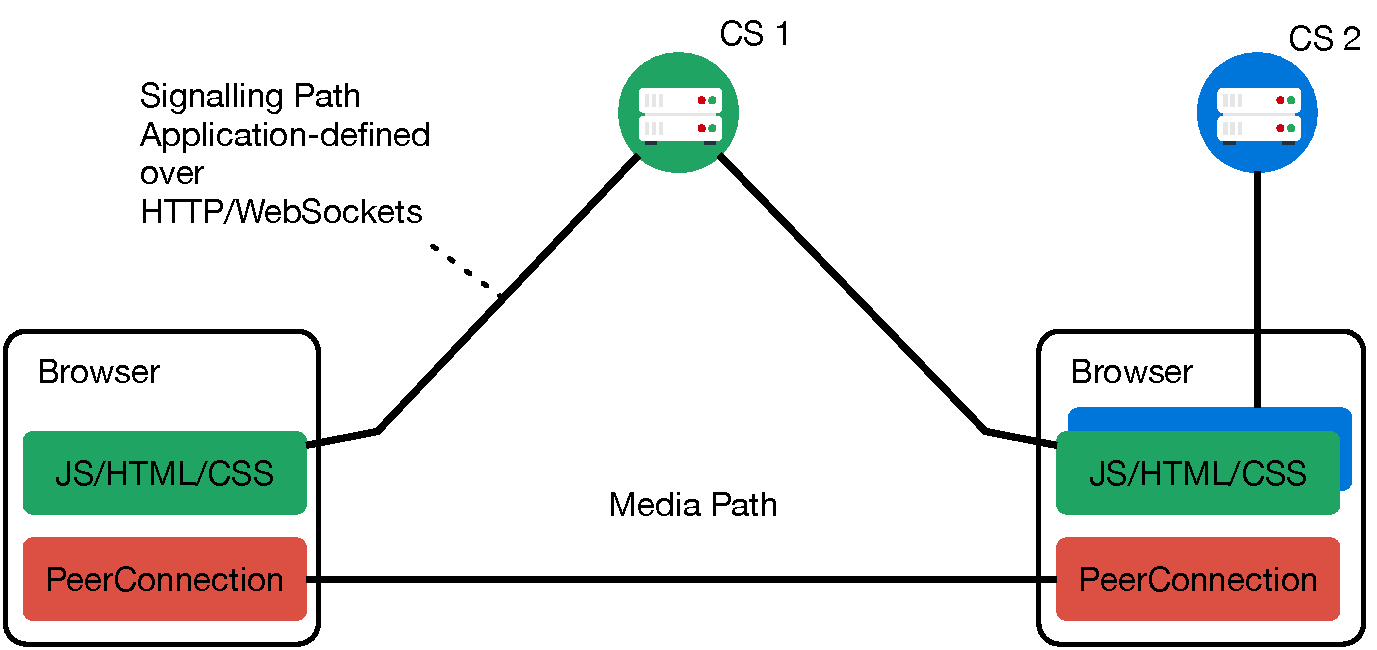
\includegraphics[width=.8\textwidth]{images/silo}
\caption[Silo Architecture]{In silo architecture users have to connect though the same \gls{cs} to establish a session.}
\label{fig:silo}
\end{figure}

Many existing companies offer \gls{voip} communication services, some of which are already switching to WebRTC\footnote{Interestingly, browsers makers porting their own communication services to WebRTC aim first at compatibility with their existing solutions and tend to implement non-standard features in their WebRTC implementation. For instance, WebRTC in Chrome supports \gls{sdes} to cater for hangouts while Edge's first video codec support was H.264 Skype's proprietary codec.}.
The only constraint for signalling is that it uses the \gls{sdp} offer/answer model.
For the moment \gls{voip} communication services on the Web are heavily relying on the silo model.
More complex architectures are being developed to allow inter-domain interoperability.
These architectures differ by the way they handle user discovery, routing, and identity management and formats.
Although the main use case for WebRTC is \gls{voip}, other services such as video streaming~\cite{nurminen2013p2p} and data sharing~\cite{vogt2013leveraging} can be supported.
In this section, we give a quick overview of some interoperable and distributed signalling architectures.

\subsection{Voice over LTE and WebRTC Interconnectivity}
\label{sec:ims}
\gls{volte} is an architecture for \gls{voip} over 4G mobile networks.
Figure~\ref{fig:volte} presents a simplified view of the \gls{lte} mobile network, a standard for high-speed mobile networks designed by the \gls{3gpp}.
This architecture is separated in an access network, \ie a network of eNodeB responsible for all radio-related functions including encryption of data sent over radio interfaces, and a core network responsible for the control of the \gls{ue} and the establishment of \gls{ip} connectivity.
In the core network, the Serving Gateway (S-GW) and Mobility Management Entity (MME) handle the \gls{ue} mobility, while the PDN Gateway (P-GW) handles \gls{ip} addresses allocation and \gls{qos} enforcement.
Finally, the Home Subscriber Server (HSS) is a database containing user's profile, location, and IP information.
It is responsible for the user authentication, subscription, and discovery.
\gls{volte} interconnects the \gls{lte} network with the \gls{ims} network.
The main goal of the \gls{ims} is to achieve the concept of Fixed Mobile Convergence\footnote{The convergence of fixed and mobile telephony networks under an All-\gls{ip} environment.}.
A simplified view of the \gls{ims} architecture is presented in Figure~\ref{fig:ims}.
\gls{cscf} form the core of an IMS domain.
The Proxy-\gls{cscf} (P-CSCF) is a \gls{sip} proxy server which serves as the point of contact for each user equipment.
When a \gls{ue} connects to a network, it looks up for a reachable P-\gls{cscf}.
In \gls{ims} roaming scenario, the \gls{ue} connects directly to the visited network's P-\gls{cscf} rather than to his home network. 

\begin{figure}[tbp]
\begin{center}
\begin{subfigure}{\textwidth}
    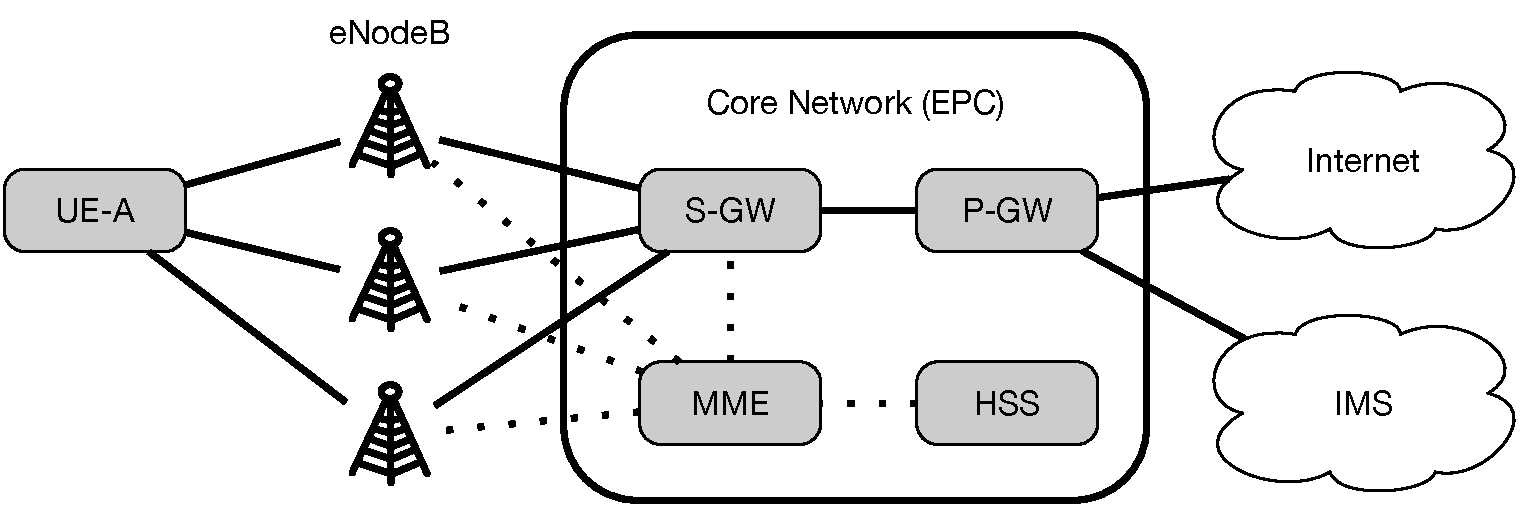
\includegraphics[scale=0.5]{images/VoLTE}
\caption{Simplified LTE architecture.}
\label{fig:volte}
\end{subfigure}\\


\begin{subfigure}{\textwidth}
    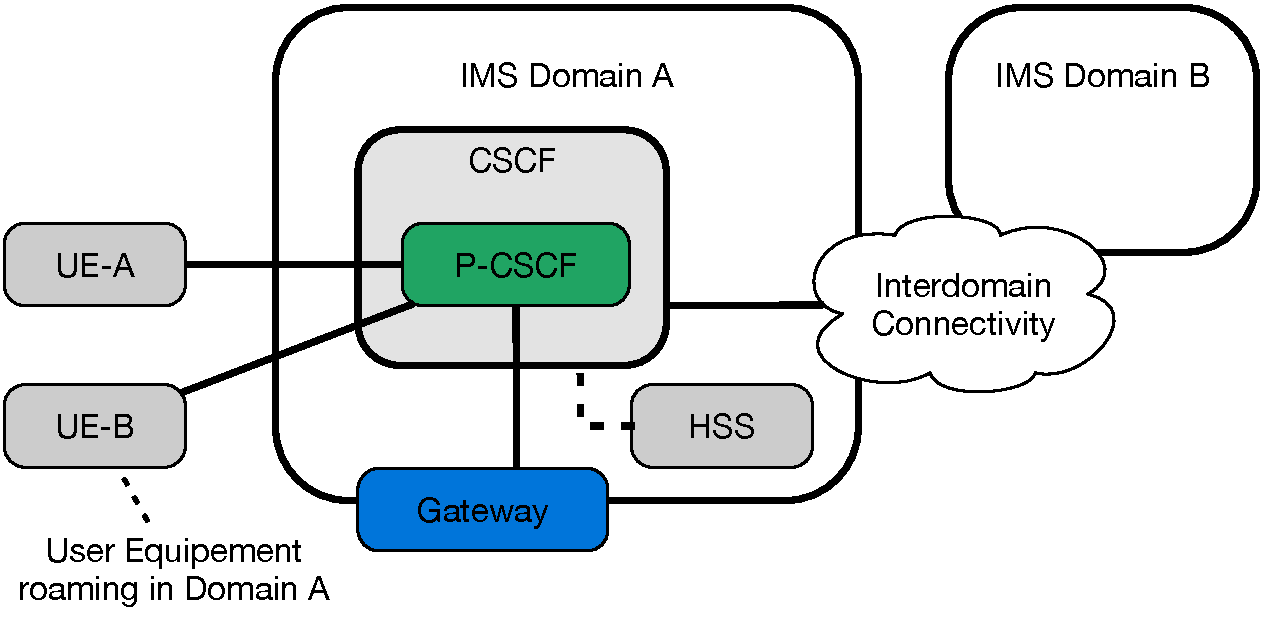
\includegraphics[scale=0.5]{images/IMSArchSimplified}
\caption{Simplified IMS architecture.}
\label{fig:ims}
\end{subfigure}
\caption[Simplified VoLTE Architecture]{A simplified view of the VoLTE architecture. The LTE offers connectivity to the Internet and to the IMS while the IMS offers VoIP service.}
\end{center}
\end{figure}

\gls{sip} is a signalling protocol supporting the determination of user location, availability, as well as session negotiation, setup, and management.
As it is only concerned with the signalling part of the communication session, \gls{sip} is used in conjunction with other protocols such as \gls{sdp} and SRTP (presented in Section~\ref{sec:webrtc}).
A network of proxy servers allows \gls{sip} endpoints to register and routes requests to a user's location.
In \gls{volte}, the \gls{ue} contains a \gls{sip} user-agent and an \gls{uicc} often refered to as a ``SIM Card''.
The \gls{uicc} contains several identity modules including the IP Multimedia Services Identity Module (ISIM) which in particular provides the \gls{ims} home domain name, a private and public identity\footnote{The public identity is a telephone \gls{uri} of the form \texttt{tel:phonenumber}.}, and a secret key used for authentication and registration.

\gls{volte} offers roaming, handover, and interconnectivity with other networks.
Interconnectivity with WebRTC can be handled by an \gls{ims} domain offering a compatible gateway (see Figure~\ref{fig:ims}).
In this case, the \gls{ims} domain has to deploy a WebRTC web server, a WebRTC JavaScript client, and enhanced functionalities for WebRTC in the P-\gls{cscf}.
The gateway performs adaptation between WebRTC and \gls{ims} protocols such as transcoding and encryption.
While encryption using \gls{dtlssrtp} is mandatory in WebRTC (see Section~\ref{sec:webrtcid}), encryption of both media and signalling is optional in the \gls{ims}.
Furthermore, as \gls{volte} security relies on the radio encryption of the access network, its \gls{rtp} profile does not support encryption.
This constraint implies that WebRTC-\gls{volte} interconnectivity cannot use End-to-End encryption with \gls{srtp} and is instead limited to End-to-Access-Edge encryption (see Figure~\ref{fig:voltesecurity}).

\begin{figure}[tbp]
\begin{center}
\begin{subfigure}{\textwidth}
    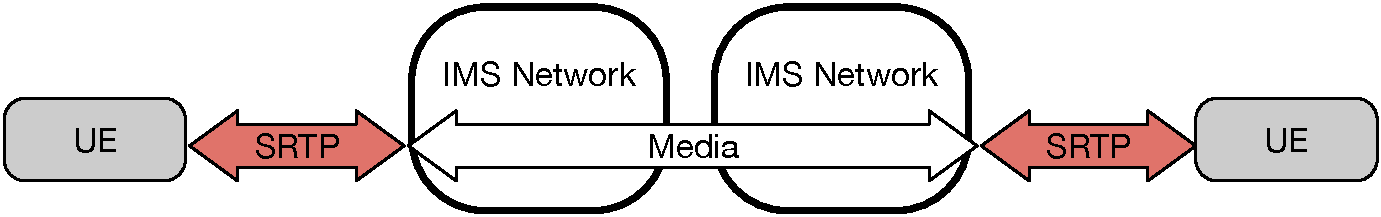
\includegraphics[scale=0.5]{images/e2aeEncryption}
\caption{End-to-Access-Edge Encryption}
\label{fig:e2ae}
\end{subfigure}\\


\begin{subfigure}{\textwidth}
    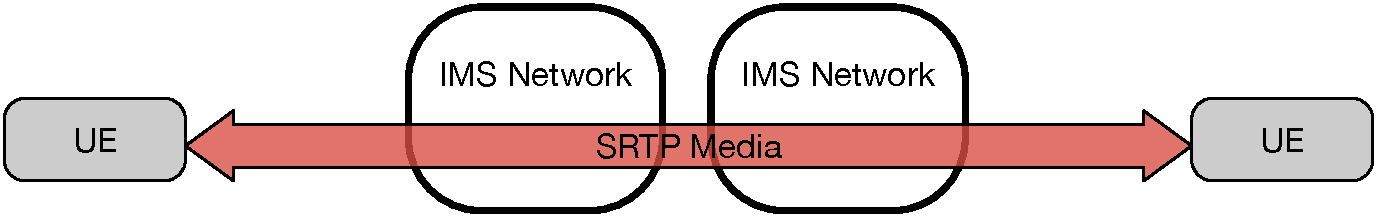
\includegraphics[scale=0.5]{images/e2eEncryption}
\caption{End-to-End Encryption.}
\label{fig:e2e}
\end{subfigure}
\caption[E2E and E2AE IMS Encryption]{End-to-End and End-to-Access-Edge encryption scenario over IMS networks.}
\label{fig:voltesecurity}
\end{center}
\end{figure}


\subsection{Matrix}
\label{sec:matrix}

Matrix~\cite{matrix} is a specification for a messaging and data synchronisation federation.
One of its use cases is the exchange of signalling message for WebRTC communications.
Figure~\ref{fig:matrix} shows three users, each connected to a Matrix home server, and exchanging synchronised message in a room. 

Matrix specifies several \gls{api}, amongst which a client-server and a server-server \gls{api}.
The server-server \gls{api} defines the \gls{http} interfaces and data format allowing Matrix home servers to synchronise messages with each other in real-time.
Servers can either push a message to another server, broadcast it to all servers in a room, or make a query to a server to get a state snapshot.
This \gls{api} also defines how servers are discovered and authenticated, and how user's presence information is exchanged between home servers.
The client-server \gls{api} defines the \gls{http} interfaces for a client application to connect and communicate with a Matrix home server.
It allows the application to manage rooms and send messages.
The client-server \gls{api} also defines how users authenticate to their home server through any Matrix application.
This particularity of the Matrix architecture means that users can choose any application to connect to any home server.

Matrix user identifiers are of the form \texttt{@UserID:HomeServerDomain}.
These identifiers are used internally by home servers, and in particular for home server discovery.
However, Matrix also defines third-party identifiers (3PID) as a more user-friendly way to refer to users.
The Identity Service \gls{api} defines how 3PID are associated to Matrix identifiers, stored, and queried.
This service relies on a trusted federation of Matrix identity servers.

Despite its interesting concepts, the Matrix ecosystem is still in early development.
Most implementations are in the alpha stage and the specification itself is rated as unstable.
The Matrix identity specification is the less advanced specification, and no identity server implementation is referenced on the Matrix webpage. 

\begin{figure}
\begin{center}
    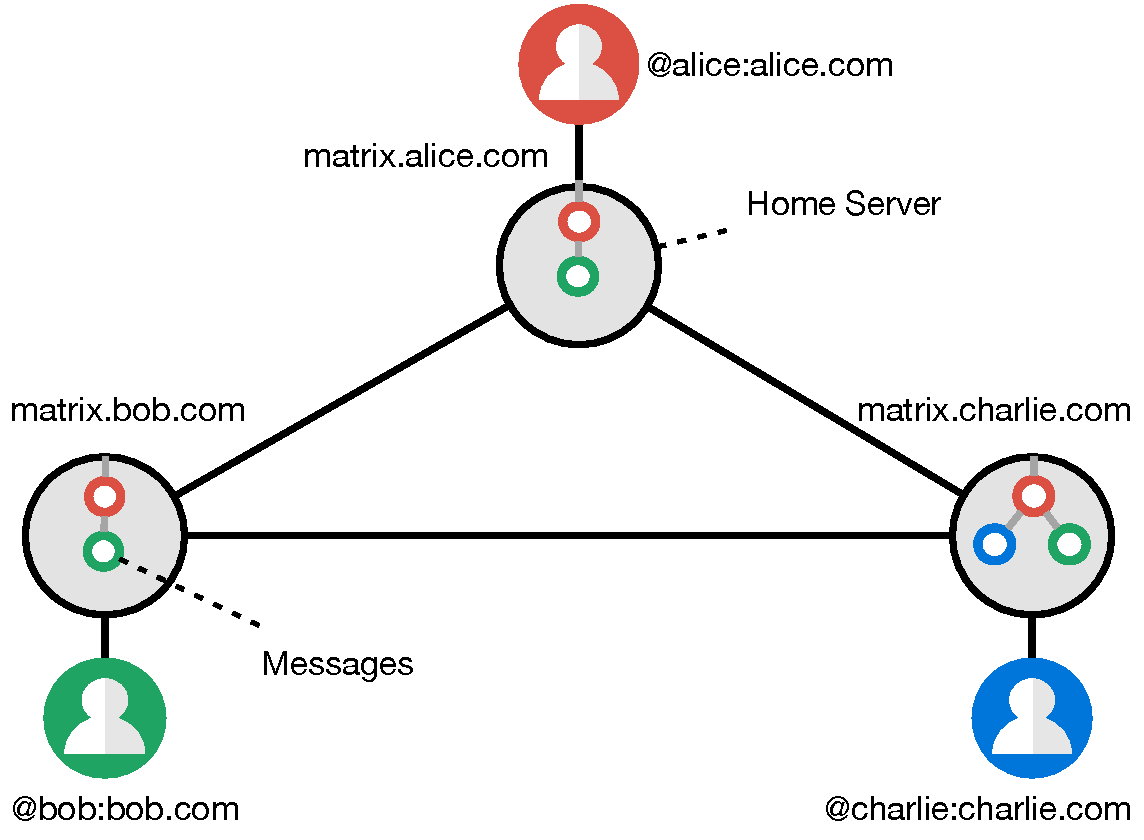
\includegraphics[scale=0.5]{images/matrixArch}
\end{center}
\caption[Matrix Messaging Federation]{Federated messaging and data synchronisation between three Matrix home servers.}
\label{fig:matrix}
\end{figure}

\subsection{reThink}
\label{sec:rethink}

reThink, an H2020 European project, specified and experimented with a real-time communication framework.
Its global objective is to allow Telcos to compete with large \gls{ott} companies by offering open and interoperable communication services and applications.

A simplified view of the reThink architecture is presented in Figure~\ref{fig:rethinkArch}.
It builds on the earlier signalling on-the-fly concept from the Wonder European project\footnote{\url{http://hypercomm.github.io/wonder/}}.
Signalling on-the-fly avoids the standardisation of messaging protocols by providing a messaging \gls{api}.
When two parties want to communicate, they agree on a protocol and download the corresponding protocol-stub implementing the messaging \gls{api}.
While this architecture allows interoperability without standards protocols, it still requires standardisation of the messaging \gls{api} and message format used for communication.

On the user's side, reThink applications are executed inside the runtime.
The runtime can be a modified web browser or a native program\footnote{The runtime was initially envisioned as a web browser modification. However, it was implemented as a JavaScript library due to the complexity and costs involved.}.
reThink applications make use of modular software components, called hyperties.
These hyperties are downloaded from service provider catalogues and executed in sandboxed environments.
Hyperties can provide many services to an application, including \gls{p2p} communications.
In the interoperable reThink architecture, users can connect to each other through different service providers.
Signalling between two hyperties is thus established through one users' service provider.
More specifically through a messaging node exposed by the selected service provider. 
In order to establish the connection, both runtimes agree on available protocols and download the corresponding proto-stub from the chosen service provider's catalogue.
This process allows hyperties to set up their session and eventually open a \gls{p2p} communication.

\begin{figure*}[tbp]
\begin{center}
    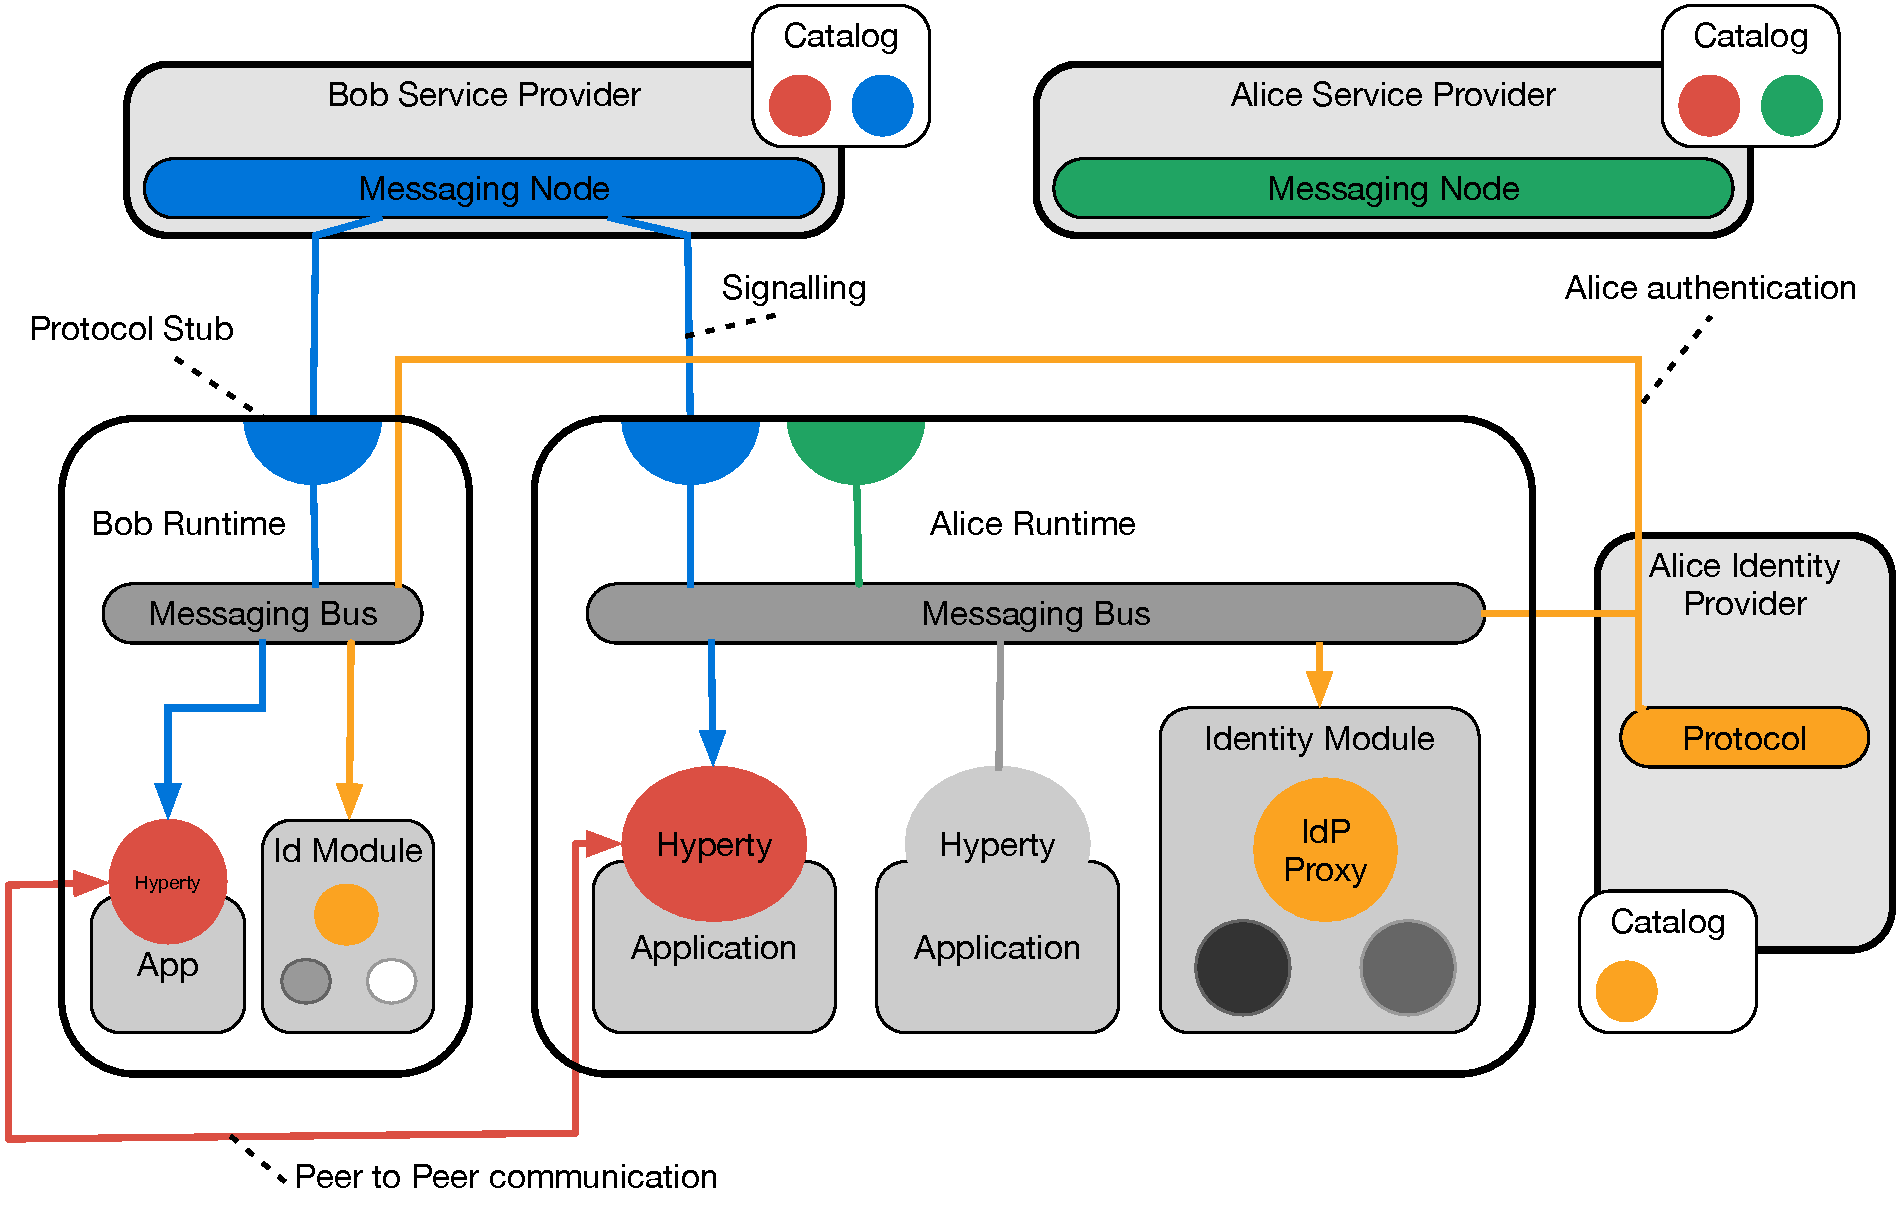
\includegraphics[scale=0.45]{images/rethinkArch}
\end{center}
\caption{Simplified reThink architecture}
\label{fig:rethinkArch}
\end{figure*}

Identity management in the reThink architecture is handled by the Identity Module and reuses the concept of the WebRTC \gls{idp} Proxy.
Some of its design objectives in addition to the WebRTC compatibility are the ability for users to choose their \gls{idp} and the availability of discovery and presence services.
In particular, reThink discovery, presented in Figure~\ref{fig:rethinkDiscovery}, is a layered architecture relying on a cryptographic \gls{guid}.
The global registry, a trusted distributed hash table run by a consortium of service providers, maps \gls{guid} to user profile information.
Users can manage and control their public profile information stored in the \gls{dht} by proving ownership of a private key.
These user profiles also point to user identities on service providers by exposing pairs of service provider domain and service bound user identifiers.
Services providers, in turn, expose a domain registry containing the user's reachability information.
\gls{guid} can either be exchanged manually or discovered through the use of a discovery service.

%reThink identity design objectives are WebRTC compatibility, \ie IdP exposing a WebRTC \gls{idp} Proxy would be also compatible with reThink, and .
\begin{figure}
\begin{center}
    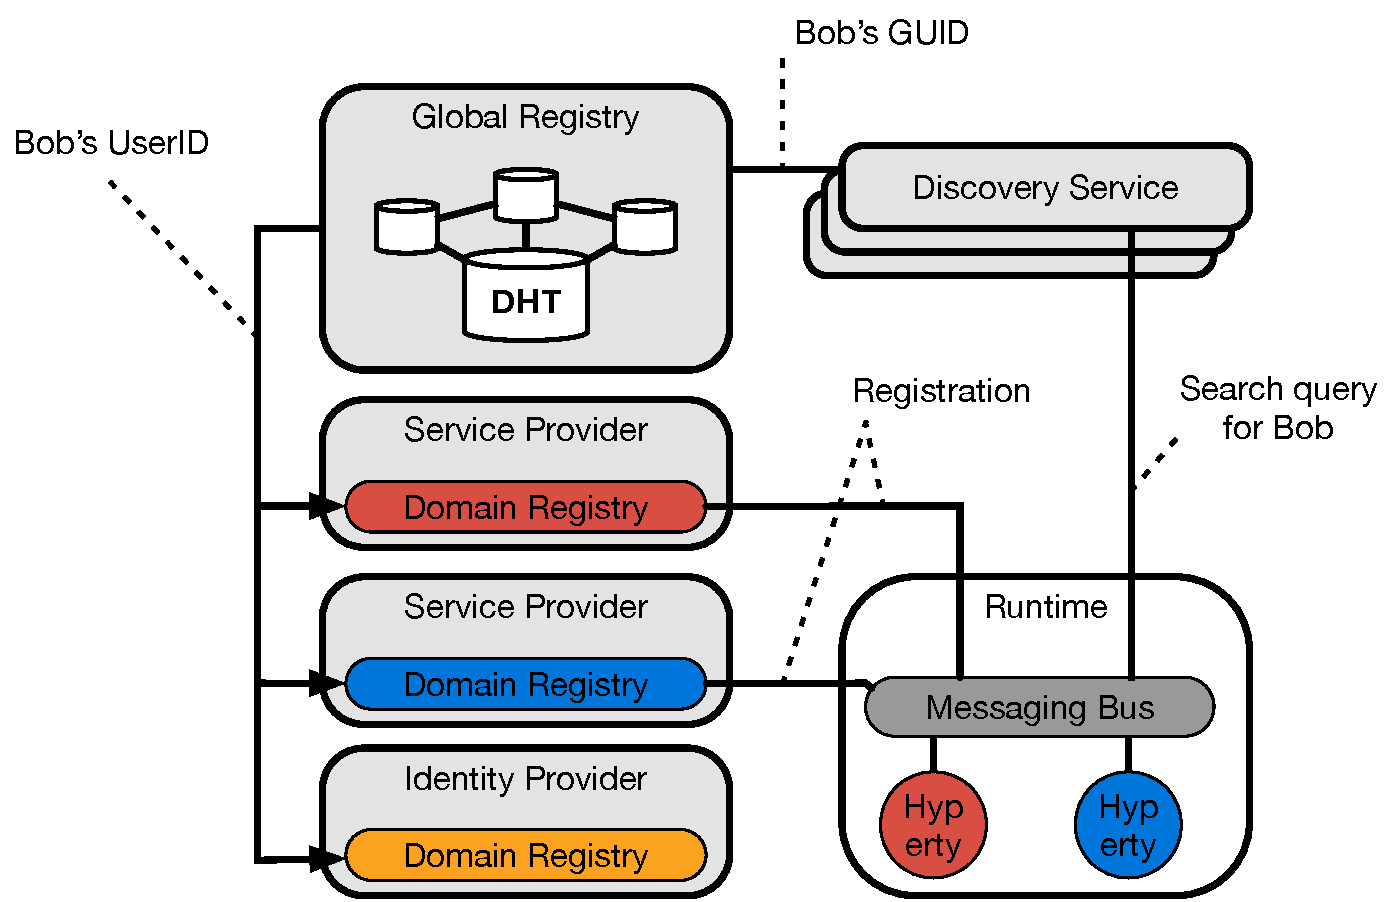
\includegraphics[scale=0.5]{images/rethinkDiscovery}
\end{center}
\caption{reThink Identity Discovery}
\label{fig:rethinkDiscovery}
\end{figure}



\subsection{Distributed Signalling Architectures}
\label{sec:spray}
The rapid growth of web traffic and video streaming, in particular, has an important impact on infrastructure costs both for content providers and network operators.
\gls{cdn} are constituted of proxy servers geographically distributed to be as close to clients as possible.
Besides tidying core network traffic, \gls{cdn} optimise the availability and performance of content delivery through various techniques and in particular caching, load-balancing, and routing techniques.
Distributed \gls{cdn} merge the advantages of \gls{cdn} and \gls{p2p} networks.
These networks leverage their clients' upload bandwidth to redistribute content to other clients and further reduce costs.
However, distributed \gls{cdn} require the installation of client-side software or browser plugin~\cite{roverso2014hive}.

WebRTC allows browser-to-browser \gls{p2p} communication for video streaming and data channels without third-party plugins.
It is thus possible to build distributed \gls{cdn} around a network of WebRTC enabled browser.
To create such network, clients first reach a bootstrapping server.
This server allows new clients to open data channels with other clients already part of the network.
These data channels form an overlay signalling network.
Once a client joined the network, it can discover other distant clients and establish \gls{p2p} connections with them, for instance, to retrieve a file or a video stream. 
Figure~\ref{fig:spray} shows an example of such network architecture where P3 joins the network and finally retrieves a video stream from P1.
As the signalling message from P3 to P1 goes through P2, the signalling architecture is similar to \gls{mitm} attack as shown in Figure~\ref{fig:mitm}.
Such signalling path may not be trusted and depending on the use case it may be an issue.
Zhang~\etal\cite{zhang2013maygh} also report some security and privacy considerations for their WebRTC \gls{cdn} framework.

\begin{figure}
\begin{center}
    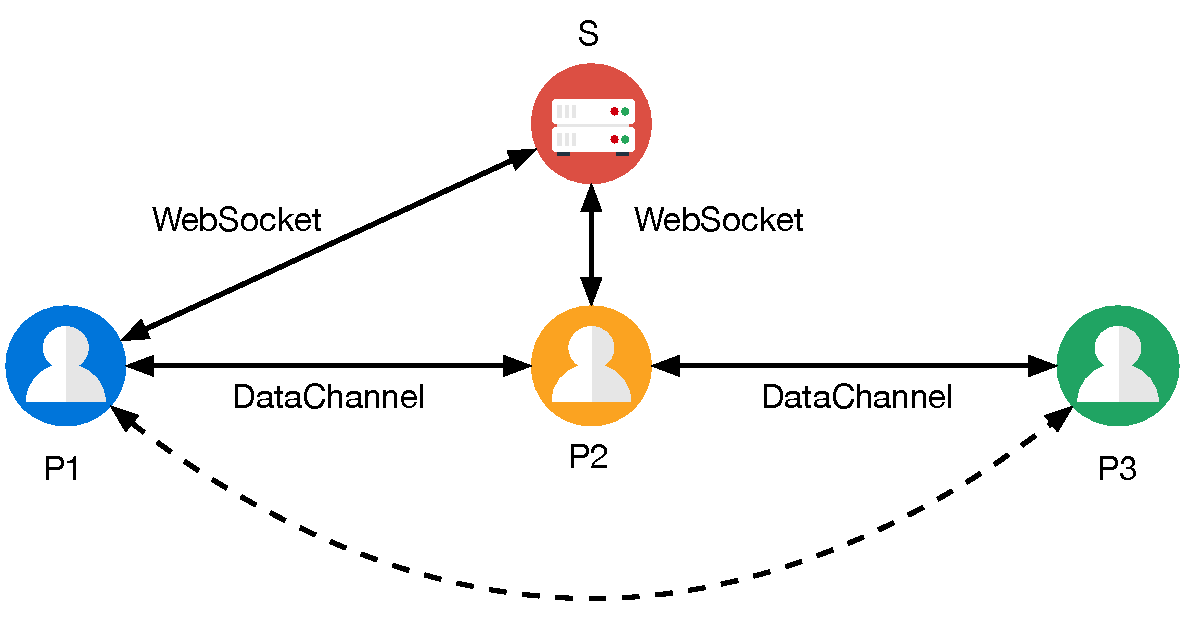
\includegraphics[scale=0.5]{images/sprayArch}
\end{center}
\caption[Spray Architecture]{In this example P1 and P2 are already part of the network. To join the network P3 first reaches the bootstrapping server S.
S signals P2 and P3 so that they open a P2P data channel. P3 then requests a video stream from P1. \gls{sdp} messages between P3 and P1 are signalled through P2 using existing data channels. Finally, the video stream is established from P1 to P3~\cite{nedelec2015spray}.}
\label{fig:spray}
\end{figure}


\clearpage
\invisiblesection{Summary}
\label{sec:contextSummary}
%\vspace*{3cm}

\blockmargin%
%\hspace{-\marginparwidth}\hspace{-\marginparsep}
\makebox[\overflowingheadlen][l]{
\begin{minipage}{\overflowingheadlen}

\begin{mdframed}[style=ContextFrame,frametitle={\ref{sec:contextSummary}~Summary}]
The WebRTC peer-to-peer media path is negotiated by peers exchanging \gls{sdp} offer/answer messages over the signalling path.
Media path encryption is mandatory and is mainly built around the \gls{dtls} and \gls{srtp} protocols. 
It ensures confidentiality and integrity of the \gls{p2p} sessions between peers.
The signalling path generally involves one or more signalling server and its security relies on standard web security protocols.
At the root of these protocols is the web browser which acts as the trusted computing base.
WebRTC applications and their associated signalling servers are also responsible to protect the availability of the session and network resources by filtering incoming call.

\medskip

Depending on the signalling architecture or the signalling servers' origin the signalling path may be untrusted by users.
WebRTC remedies to this issue by allowing peers to bind \gls{dtls} certificates to identity assertions.
These assertions are generated and verified by identity providers forming two symmetric identity paths.
Paradoxically, these identity paths are configured by the communication services.

\medskip

Privacy is a growing concern for users and contributors of web specifications alike.
The main privacy threats against WebRTC users are related to identification of anonymous callers and correlation of web browsing and call history.
Browsers enforce consent policies to protect users against malicious sites launching non-legitimate calls.
However, legitimate communication services also gain an important knowledge of their users' call history.

\medskip



\end{mdframed}

\end{minipage}
}
\unblockmargin

%
%
%\todo{Should we conclude the summary by a reference to the research questions? Given the responsibility of actors of the call setup related to the security and privacy of WebRTC communications, users should be able to choose trusted actors and understand to which level is their security guaranteed. At the moment, the WebRTC trust model is quite informal. and so on.}

\chapter{State of the Art}
\label{sota}
\label{sec:secandtrust}

%%%%%%%%%%%%%%%%%%%%%%%%%%%%%%%%%%%%%%%%%%%%%%%%%%%%%%
%%%%%%        MODELLING SECURITY AND TRUST
%%%%%%%%%%%%%%%%%%%%%%%%%%%%%%%%%%%%%%%%%%%%%%%%%%%%%%
\begin{quote}
\textit{
In this chapter, we present the state of the art on \gls{voip} security research.
In Section~\ref{sota2012} we present the results of a survey reviewing 245 articles on \gls{voip} security and published in 2012 by Keromytis~\cite{keromytis2012comprehensive}.
As the first drafts of WebRTC specifications were published the same year, this survey is a solid starting point to understand the field of \gls{voip} security.
In Section~\ref{sec:sota2012+}, we present our own survey of \gls{voip} and WebRTC security research papers published between 2012 and 2017.
We follow a similar methodology as used by Keromytis and collect and classify 208 papers.
We then review the papers dealing specifically with WebRTC.
}
\end{quote}
\glsresetall
\section{VoIP Security Research - 2012}
\label{sota2012}
WebRTC is in 2018 still a young technology.
The \gls{w3c} WebRTC Working Group was created in May 2011 and the first version of the WebRTC Security Architecture draft was published in January 2012.
The same year, Keromytis published ``A Comprehensive Survey of Voice over IP Security Research''~\cite{keromytis2012comprehensive} which reviews 245 articles related to fields of \gls{voip} security.
This survey is a starting point for understanding the field of \gls{voip} security research just before the introduction of WebRTC. 
Indeed, WebRTC contributors built on the same accumulated experience when making design and implementation decisions.

In this section, we summarise Keromytis' survey and categorisation of \gls{voip} research topics.
We also give additional references from our personal knowledge when it seems relevant.
We particularly focus on research that could be applied in the context of WebRTC communication.
Note that a large part of the security research on \gls{voip} is focused on the network side such as the \gls{sip} signalling protocol and \gls{sip}-based architectures.
While WebRTC does not mandate a particular signalling architecture, \gls{sip}-based researches are still relevant to WebRTC.
Actually, \gls{sip} could be used on the signalling path, but more importantly, most vulnerabilities and defence mechanisms related to \gls{sip} are still relevant for ad-hoc signalling protocols.

\subsection{Threats Classification and Methodology}
\label{keromytis}
To build the survey, Keromytis initially collected papers from personal knowledge, searches on online library\footnote{CiteSeer, IEEE Xplore, ACM Digital Library, and Google Scholar.}, and browsing of proceedings of top security conferences, journals, and specific workshops\footnote{IEEE Security \& Privacy Symposium, ISOC Symposium on Network and Distributed Systems Security, ACM Computer and Communications Security, USENIX Security, RAID, ACM Transactions on Information and Systems Security, and IEEE Transactions on Dependable and Secure Computing.}.
In particular, searches were conducted with the following keywords: ``VoIP security'', ``VoIP vulnerabilities'', ``VoIP attacks'', ``SIP security'', ``SIP vulnerabilities'', and ``SIP attacks''.
The collection was then expanded by browsing the proceedings of conferences in which these papers appeared and searching for other VoIP security papers by the same authors.
The process was iterated over until no new papers were added to the collection.

These papers were then manually classified according to an extended version of the \gls{voipsa} threat taxonomy~\cite{zar2005voip}.
The considered \gls{voipsa} threat classes are the following: social threats, traffic attacks, denial of service, and service abuse.
In addition, eight additional classes were considered: overviews and surveys, field studies and system/protocol analysis, performance analysis, authentication protocols, architectures, middleboxes, intrusion detection, and miscellaneous. 
Figure~\ref{fig:keromytis} presents the repartition of surveyed papers in these classes.

\begin{figure}
\begin{center}
    
\includegraphics[scale=.5]{images/keromytis}
\end{center}
\caption{Classification tree~\cite{keromytis2012comprehensive}}
\label{fig:keromytis}
\end{figure}


\subsection{Keromytis Survey Summary}
\subsubsection{Social Threats}
Social Threats represent the attacks aimed at the human users rather than at the software systems.
Such attacks are for instance unwanted contacts misrepresenting the identity of a malicious calling party or bypassing opt-out consent.
In practice, research on social threats is mostly focused on defence against \gls{spit} call which we presented in Section~\ref{sec:availability}.

According to the \gls{voipsa}, the classification of call as spam is subjective. 
Indeed, \gls{spit} call may be lawful solicitations and become spam only after bypassing refused consent.
The bulk of defence against \gls{spit} thus focus on getting user's input.
Caller classification may follow a simple binary approach into whitelists or blacklists.
However, more complex approaches propose to use reputation-based models and social relations between users to assign a trust value to an incoming call.
In these systems, the intelligence of \gls{spit} detection algorithms is located at the endpoints and allow users to manage their own policies for \gls{spit} rejection.

Other approaches place \gls{spit} detection at the network level, \ie on the signalling path.
These systems measure various criteria such as the number of incoming and outgoing calls, call duration, and call history.
Deviation from standard long-term expected average may reveal a spam call.
These analyses may further be refined by user input or filtered with a Turing test\footnote{Turing tests tries to distinguish computers from humans.} presented to the caller.
Some authors also propose to apply fingerprinting techniques, either targeting \gls{sip} messages format or the audio data of incoming \gls{voip} calls.
\gls{spit} calls would be detected by the presence of unique fingerprint over a large number of different calls.
Sorge \etal\cite{DBLP:conf/icc/SorgeS09} propose to evaluate the reputation of \gls{cs} and their \gls{spit} detection algorithms, providing incentives to honest \gls{cs} to correctly tag outgoing calls.

Trust and reputation models may easily be bypassed under weak caller authentication.
Some authors thus propose to enforce strong caller identity verification.
In particular, Srivasta \etal\cite{srivastava2004preventing} propose to consider the caller origin domain and the confidence level in the authentication performed while Croft \etal\cite{croft2005model} propose to include a Verifying Authority into the call setup.
This Verifying Authority would be responsible for applying policies in particular based on the caller identity before transmitting the call to the user.

\subsubsection{Traffic Attacks}
The traffic attacks and defences class is concerned with the risks of eavesdropping, interception, and modification of signalling data and media sessions.
These attacks may either target unencrypted sessions or bypass cryptographically protected sessions.
This field of research, however, does not consider generic cryptography research but only focus on specific \gls{voip} cases.

Indeed, the specific nature of \gls{voip} traffic, transmitting voice in stream sessions, may allow specific attacks.
Some researchers thus propose to use packet delay variation (also referred to as jitter) in order to de-anonymise \gls{voip} streams or introduce covert channel.
Other researchers apply machine learning techniques to determine the language spoken or identify blank, phrases, or even words in encrypted voice streams.
As summarised in Figure~\ref{fig:vbrRecognition}, these attacks use packet size variation of \gls{vbr} human-speech codecs.
\gls{vbr} codecs, as opposed to Constant Bit Rate codecs, use variable packet size depending on factors such as encoded phonemes, blank in speech, or encoding quality.
As \gls{voip} is a time-sensitive application, delay or jitter may have a dramatic impact on the availability of the communication.
Thus reducing bandwidth usage and adapting to network conditions is a critical feature for \gls{voip} usability.
However, these researches reveal a trade-off between security and availability/quality of \gls{voip} communications.
\gls{rfc}~6562~\cite{RFC6562} gives guidelines on the usage of \gls{vbr} codecs in conjunctions with \gls{srtp} sessions.

\begin{figure}
\begin{center}
    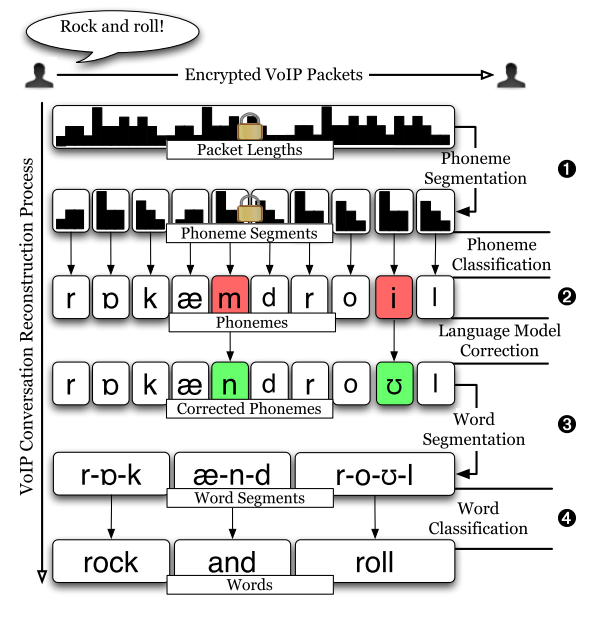
\includegraphics[scale=.5]{images/vbrRecognition}
\end{center}
\caption[VBR Transcripts Reconstruction]{Overall architecture of an approach for reconstructing transcripts of \gls{voip} conversations from sequences of encrypted packet sizes~\cite{White2011}.}
\label{fig:vbrRecognition}
\end{figure}

Traffic analysis and signalling data can be used to compromise users' privacy.
Some researchers study approaches based on anonymisation networks such as Tor (see Section~\ref{sec:tor}) and traffic padding techniques~\cite{DBLP:conf/acsac/MelchorDI07,DBLP:conf/cms/ZhangF10, }. 
Srivasta~\etal\cite{DBLP:conf/sp/SrivatsaLI08} study the issue of \gls{qos}-sensitive routes in anonymising networks. 
To this day, QoS is still an issue for \gls{voip} over anonymisation networks and researchers are still exploring possible solutions~\cite{DBLP:journals/popets/HeuserRPCDEKST17}.

A number of researches suppose unencrypted signalling paths or media session or focus on alternative key agreement protocols such as ZRTP. 
As WebRTC mandates the use of \gls{dtls} and \gls{srtp} for media and data sessions, and browsers enforce the use of \gls{tls} for signalling session, we do not consider these results as relevant to our research.

\subsubsection{Denial of Service}
We presented \gls{dos} attacks in Section~\ref{sec:availability}.
While \gls{dos} attacks may target either endpoints or networks elements, researches in this field mostly focus on attack and detection at the network level.
\gls{dos} flooding attacks, schematised in Figure~\ref{fig:dos}, have similarities to \gls{spit} calls meaning that these can be detected by monitoring deviation from standard call frequencies or error rate. 
Legitimate situations such as emergencies may also conduct to flooding scenarios.
Some researchers thus try to differentiate \gls{dos} attacks from flash crowds situations~\cite{DBLP:conf/ccs/FuchsALM08}.
However, the main difference with \gls{spit} is that \gls{dos} attacks aim at shutting down the \gls{voip} network.
It is crucial for detection algorithms to introduce as few overheads as possible during call setup.

Indeed, other \gls{dos} attacks directly aim at flooding the memory or CPU of network elements and in particular \gls{sip} servers.
While strong message authentication is proposed as a solution against \gls{dos} attacks, some researchers show that authentication may have a negative impact in some \gls{dos} scenarios~\cite{DBLP:conf/noms/LuoPL08}. 
Whitelisting or lightweight authentication based on call history from regular caller's identity or \gls{ip} adress, actually similar to some trust models, are proposed to mitigate attacks.
Other mitigation techniques also propose to adapt server procedures during \gls{dos} scenarios, for instance, dropping ringing call earlier when being overloaded~\cite{DBLP:conf/ism/ConnerN08}.

\begin{figure}
\begin{center}
    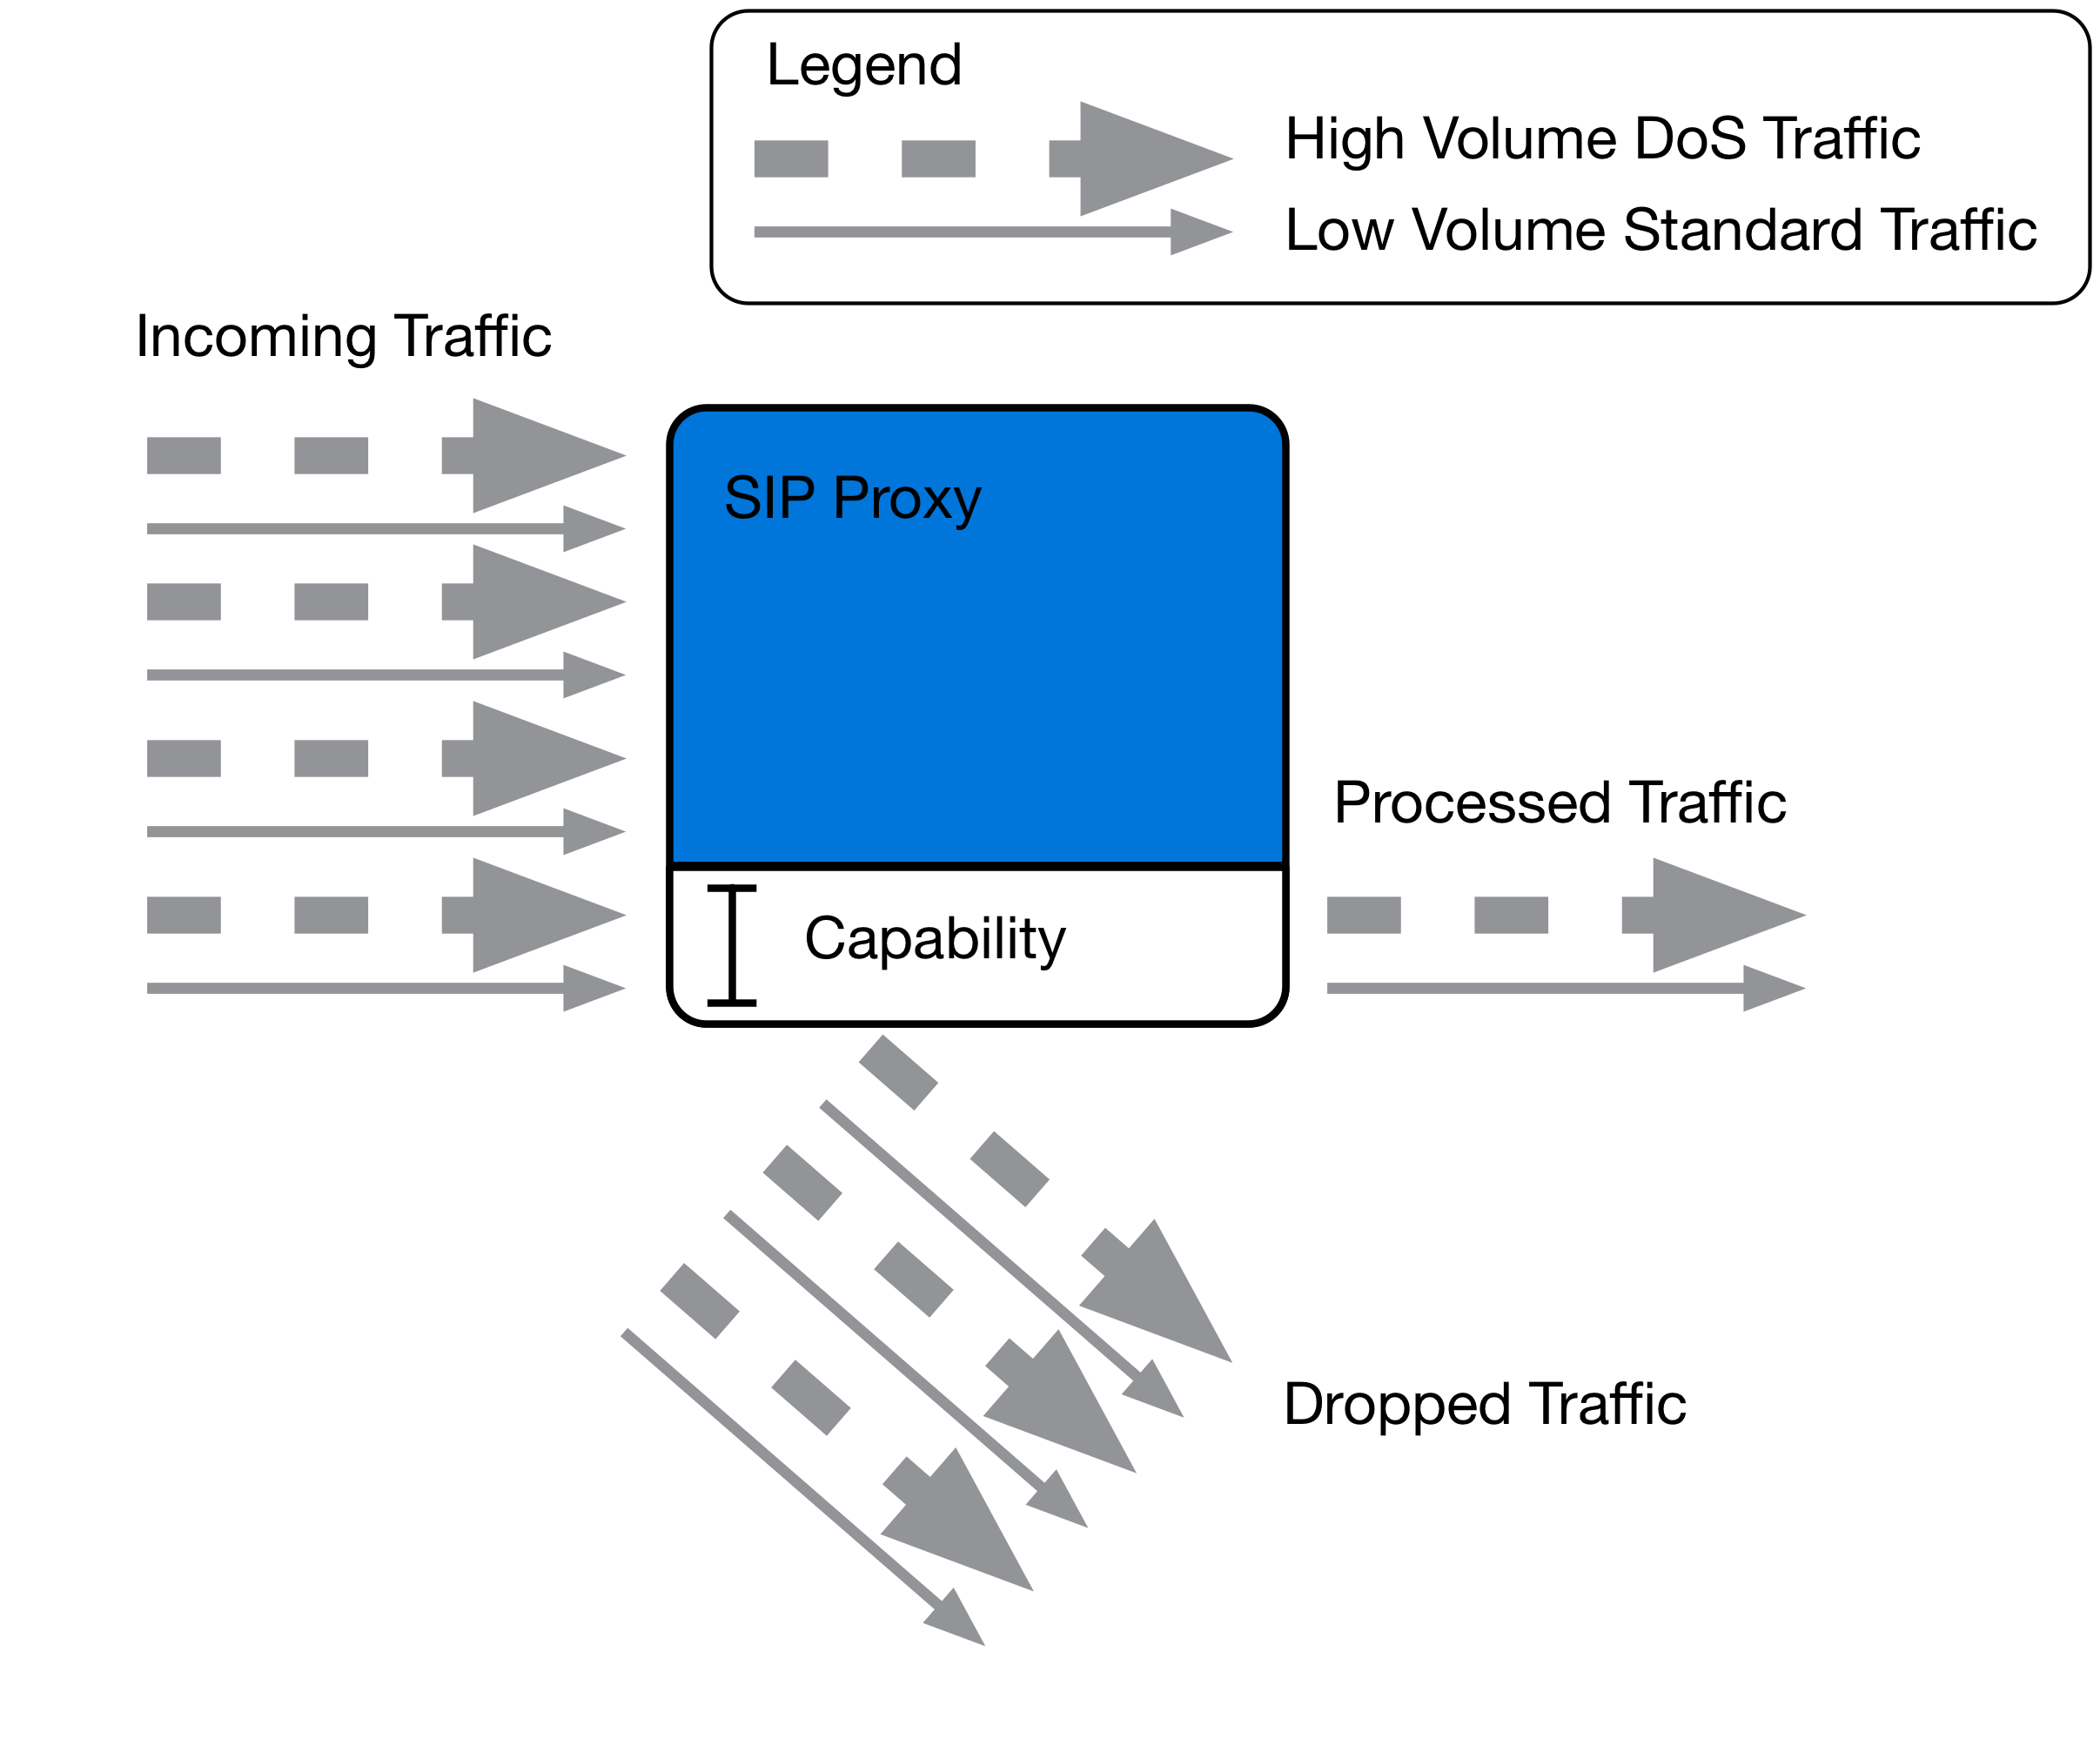
\includegraphics[scale=.5]{images/dos}
\end{center}
\caption[Denial of Service Flooding Attack]{Schematic overview of a \gls{dos} flooding attack. Due to the server's limited processing capabilities a lot of regular requests cannot be processed if a high load of malicious messages are targeted towards the server~\cite{ehlert2010survey}.}
\label{fig:dos}
\end{figure}

Payload and flow tampering attacks target specific signalling protocols, respectively to crash servers or abort sessions.
Most research on these attacks focus on \gls{sip} and protection mechanisms are well-known~\cite{ehlert2010survey} including tools to check \gls{sip} implementations.
Additionally, encryption on the signalling path deters flow tampering attacks.


\subsubsection{Service Abuse}
Service abuse threats are related to the improper use of \gls{voip} services especially in commercial services, for instance, to increase or avoid billing.
The research in this area is quite limited compared to other threat classes as it features only 7 references.
This can be explained by the specificity of architectures concerned by service abuse threats.
Billing is closely associated with authentication and authorization of users.
Some described attacks use a \gls{sip} protocol vulnerabilities revealed by formal verification to forge \gls{sip} messages impersonating users.
A solution to fraud and proposed by Geneiatakis \etal\cite{geneiatakis2008mechanism} is to let an \gls{aaa} server sign \gls{sip} messages after the user authenticated to the server, hence providing authenticity and non-repudiation for signalling messages. 
Although the solution is based on Telco rather than web protocols, it shows similarity to the introduction of a third-party \gls{idp} in WebRTC communication setup.


\subsubsection{Field Studies and System/Protocol Analysis}
Researches in this category focus on analysing protocols, implementations, and deployed systems using various techniques in order to find security vulnerabilities and flaws. 
Techniques used include formal verification~\cite{DBLP:conf/csfw/GuptaS07}, fuzzy testing~\cite{DBLP:conf/im/AbdelnurSCP07}, as well as black-box~\cite{DBLP:conf/infocom/BasetS06} or source code analysis~\cite{berson2005skype}. 
Similar analyses are also conducted in paper classified in other categories.

Formal verification techniques ensure that supposing a defined attacker model, the attacker cannot learn compromising information.
Such an attacker model is the Dolev-Yao~\cite{dolev1983security} model in which the attacker can listen to any message on the network, build arbitrary messages from known information, and send them over to the network.
The AVISPA project\footnote{\url{avispa-project.org}}, for Automated Validation of Internet Security Protocols and Applications, is a suite of tools for formal modelling and verification of security protocols.
In particular, the project offers a library of protocol models in the High-Level Protocol Specification Language, some with known and demonstrated attacks.

Formal verification should not hide the fact that actual implementations may present faults and weaknesses. 
These faults may be due to weak specification, error in the implementation, or use of default configurations.
For instance the Heartbleed bug\footnote{\url{heartbleed.com}} allowed an attacker to reveal the memory of an OpenSSL protected system, the most popular \gls{tls} implementation, by using a missing bound-check in the handling of the \gls{tls} heartbeat\footnote{The actual fix shows how a small implementation error can have dramatic consequences: \url{https://git.openssl.org/gitweb/?p=openssl.git;a=commitdiff;h=96db902}}.

A number of surveyed work resulted in vulnerability disclosure publications in databases such as the \gls{cve} database.
Such database allows the rapid dissemination of vulnerability disclosures and fixes to organisations using security software.


\subsubsection{Performance Analysis}
Performance analysis works focus on evaluating the impact of security protocols on both call setup and media sessions.
We already mentioned the trade-offs between security and availability/quality of the communications.
Papers in this category try to precisely measure this trade-off.

Results globally show that the main overhead is due to the asymmetric encryption of signalling messages while the symmetric encryption of the media session only produces a small overhead.
The exact figures vary depending on the actual protocol and configurations being compared.
For instance, a prototype demonstrates an improvement from a factor between 2 and 8 in handled call setup requests per second by using the Elliptic Curve DSA algorithm instead of RSA.

Other researches, not referenced in the survey, evaluate the strength of cryptographic protocols.
In practice, perfect security is highly impracticable and only imperfect security can be achieved~\cite{Shannon1949}.
Modern cryptography thus aims for a high enough security given reasonable computation power. 
Guessing attacks (or brute-force) form an upper-bound to the amount of computation required to break an encryption.
Against some encryption schemes, faster techniques than exhaustive search can be used.
To estimate the difficulty of an attack against these encryptions it is necessary to factor computation time and cost in the equation. 
For instance, Kleinjung et al.~\cite{Kleinjung2012} use Amazon cloud public prices to compare the security level of current algorithms with the level of the DES in 1980, as proposed by Lenstra~\cite{Lenstra2004}. 
As the computing power increases and computing cost decreases over time these estimations must be updated regularly. 
National security agencies~\cite{ANSSI, NIST} also give recommendations on security algorithm implementations and usages to achieve reasonable security properties in a given timeframe.

Alia \etal\cite{alia2010putting} propose a component-based adaptation model to manage the trade-offs between \gls{qos} and Security.
They model the adaptable \gls{voip} system as a composition of components each providing different \gls{qos} and security properties.
A utility function aggregating \gls{qos} and security dimensions, shown in Figure~\ref{fig:utilityFunction}, allows discriminating between different configurations.
Considered dimensions are the latency and video scheme quality for \gls{qos} and the confidentiality, anonymity, and authentication for security.
Their model also uses user's preferences as weight in the utility function and risk context as minimal required value for each security dimensions.

\begin{figure}[H]
\begin{center}
$U = W^{lat}.F(lat) +  W^{qua}.F(qua) + W^{conf}.F(conf) +$\\

$ W^{anon}.F(anon) + W^{auth}.F(auth)$
\end{center}
\caption[Alia~\etal\cite{alia2010putting} Utility Function]{Overall utility function~\cite{alia2010putting} with $F(k)$ the utility functions and $W^k$ the user preference weights for dimensions $k$ as latency, video scheme quality, confidentiality, anonymity, and authentication.}
\label{fig:utilityFunction}
\end{figure}

\subsubsection{Authentication Protocols}
The \gls{sip} authentication mechanism is based on \gls{http} digest authentication~\cite{RFC3261} and allows any \gls{sip} proxy or \gls{sip} user-agent to issue an authentication challenge when receiving a request. 
The response to the challenge is basically a hash of some information including a nonce, \ie a unique random number associated with the request, and a password.
The response also includes a username.
Upon receiving the response, the entity which issued the challenge looks up the password corresponding to the submitted username. 
It can then perform the same digest operation and compare the result to the given digest response to validate it.

Researchers working on authentication protocols mainly propose extensions or variants to \gls{sip} authentication and are mostly focused on \gls{voip} as a use case for cryptography.
Interestingly, an article published by Cao and Jennings~\cite{cao2006providing} in 2006 deals with the issue of end-to-end user identity in \gls{voip} call establishment.
One of their assumptions is that using TLS over each signalling hop is unrealistic\footnote{The authors explains this as to be ``because of some difficulties and other reasons for deploying TLS''~\cite{cao2006providing}.}, thus breaking the necessary chain of trust.
In 2017 this assumption cannot be considered valid anymore and the WebRTC security architecture recommends for the signalling path to be secured by TLS\footnote{``[The signalling] message is sent to the signalling server, e.g., by XMLHttpRequest or by WebSockets preferably over TLS''~\cite{I-D.ietf-rtcweb-security-arch}.}.


\subsubsection{Other categories}
Other research surveyed by Keromytis are categorised as middleboxes, architectures, and intrusion detection aiming at various threats but ``not easily classified in any of the previous categories''.
Middleboxes are network devices manipulating traffic for other purposes than packet forwarding.
Researches on \gls{voip} middleboxes thus focus on the traversal and operation of firewall and gateways to other networks.
Architecture and intrusion detection researches mainly focus on the detection of anomalies in \gls{voip} networks, either from malicious or non-adversarial causes and related defences.


\subsubsection{Observations}
According to Keromytis observations, almost 20\% of the surveyed publications offer an overview of \gls{voip} security problems and solutions.
He also observes that over 15\% of the work is coming from the cryptographic community, either to increase security or performance and that roughly 20\% of researches are dedicated to addressing \gls{spit}.
While he remarks that \gls{spit} is not currently an issue for \gls{voip}, he adds that prior and current experiences in email and telemarketing spams should be sufficient motivations to continue researches against \gls{spit}.

Comparatively, he observes that the problem of \gls{dos} is less studied and that researches on the subject focus on the network side of things. 
In previous surveys on the \gls{cve} database, Keromytis reported a majority of \gls{sip}-specific \gls{dos} vulnerabilities with half of the \gls{dos} vulnerabilities present at the endpoint.
He thus argues for more research targeting this problem, especially looking at strengthening implementations and not addressing the problem from a black-box approach.
Finally, Keromytis also argue for more work addressing cross-protocol and cross-implementation problems.


\section{VoIP and WebRTC Security Research - 2012+}
\label{sec:sota2012+}
\label{sec:vapen}
To complete our state of the art we survey and categorise \gls{voip} research and published since 2012.
We first present our methodology for collecting papers.
We then give a rough overview of the repartition of \gls{voip} research since 2012 by classifying collected papers.
Finally, we review collected papers dealing specifically with WebRTC.

\subsection{Methodology}
To build our survey we first look at collecting papers related to \gls{voip} security research and published between 2012 and 2017.
We use the same keywords as Keromytis~\cite{keromytis2012comprehensive}, that is: ``VoIP security'', ``VoIP vulnerabilities'', ``VoIP attacks'', ``SIP security'', ``SIP vulnerabilities'', and ``SIP attacks''. 
As WebRTC was introduced in 2012 and is the focus of our research, we also look for papers specifically targeting WebRTC.
To this end we use WebRTC as an additional keywords, \ie ``WebRTC security'', ``WebRTC vulnerabilities'', ``WebRTC attacks''.
The search is finally conducted on Google Scholars search engine and using the search strings presented in Figure~\ref{fig:searchString}.

\begin{figure}[H]
\begin{center}
``VoIP OR SIP OR WebRTC Security OR Vulnerabilities OR Attacks ''\\

``WebRTC Security OR Vulnerabilities OR Attacks ''
\end{center}
\caption{Paper collection search strings used on Scholar.}
\label{fig:searchString}
\end{figure}

Google Scholar indicates 27 800 results for the first search string and 2 890 results for the second string.
We crawl these results, ordered by relevance until we estimate that proposed papers are not relevant anymore.
Paper selection is done based on title and abstract, and ultimately our paper collection on \gls{voip} research returns 208 results.
We do not consider non-peer reviewed papers. Relevant \gls{rfc} are presented in the background Chapter~\ref{security} on WebRTC trust and security architecture. 

\subsection{Observations on VoIP Security Research since 2012}

\begin{table}
\begin{tabular}{{@{}lcccc@{}}}\toprule\toprule
  \textbf{Category} & \textbf{-/2012} & \textbf{2012/2017} & \textbf{diff} & \textbf{WebRTC} \\\midrule
  \textbf{Denial of Service} & $12.6\%$ (31) & $16.4\%$ (33) &  $+ 3.8\%$ & $0$ \\
  \textbf{Service Abuse} &$  2.9\%$ (7) &$ 5\%$ (10) &$ + 2.1\% $& 0\\
  \textbf{Social Threats} &$ 17.5\%$ (43) &$ 6.5\%$ (13) &$ - 11\% $& 1 \\
  \textbf{Traffic Attacks} &$ 12.2\%$ (30) &$ 5\%$ (10) &$ - 7.3\% $& 2 \\\midrule
  \textbf{Overviews and Surveys} &$ 20.4\%$ (50) &$ 15.9\%$ (30) &$ - 4.5\% $& 7 \\
  \pbox{20cm}{\textbf{Field Studies and} \\ \textbf{System/Protocol Analysis}} &$ 4.9\%$ (12) &$ 8.9\%$ (18) &$ + 4\% $& 2 \\
  \textbf{Performance Analysis} &$ 5.7\%$ (14) &$ 7.5\%$ (15) &$ + 1.8\% $& 0 \\
  \textbf{Authentication Protocols} &$ 6.1\%$ (15) &$ 16.4\%$ (33) &$ + 10.3\% $& 1 \\
  \textbf{Architectures} &$ 7.7\%$ (19) &$ 10.4\%$ (21) &$ + 2.7\% $& 8 \\
  \textbf{Middleboxes} &$ 4.5\%$ (11) &$ 1\%$ (2) &$  - 3.5\% $& 2\\
  \textbf{Intrusion Detection} &$ 4.5\%$ (11) &$ 4.5\%$ (9) &$ - $& 0\\
  \textbf{Miscellaneous} &$ 0.8\%$ (2) &$ 2.5\%$ (5) &$ + 1.7\% $& 0 \\\midrule
  \textbf{Total} & 100\% (245) & 100\% (201) & & 23\\\bottomrule
  \hline
\end{tabular}
\caption{Classification of VoIP security papers returned by our search.}
\label{tab:classificationPaper}
\end{table}

We roughly classify our collection of 208 papers, based on title and abstract, into the same categories as presented in Section~\ref{keromytis}.
This allows to compare the proportion of results for both periods and get a picture of the repartition of researches.
Table~\ref{tab:classificationPaper} shows the classification of collected papers and compare them with the repartition of paper collected by Keromytis.

According to our classification, we observe some significant changes ($> +/-5\%$) in the repartition of research.
Firstly, we observe a drop in the proportion of research focusing on social threats by $11\%$ for the period since 2012. 
Keromytis remarked that most of the social threat researches were focused on \gls{spit} mitigation, although it was not an issue in \gls{voip} yet. 
This fact may explain the decrease in research for this threat category.
Researches focused on traffic attack also decreased by more than $7\%$ on the same period.
In particular, we do not observe any research related to traffic attack since 2016 and we classify only one 2015 paper as traffic attack related.
Conversely, the authentication protocol category of research sees an increase of more than $10\%$.
In particular, we collected multiple papers applying elliptic-curve cryptography to \gls{voip} while in Keromytis's survey only two references are given.
Note that some of these differences may be due to the way we collected and classified papers compared to Keromytis process.

We then looked for references to WebRTC in surveyed papers.
We extracted a list of authors of these WebRTC security papers and looked for any missing publications using DBLP\footnote{\url{dblp.uni-trier.de}}, revealing two additional overview papers.
Unsurprisingly, the categories of Denial of Service, Service Abuse, and Intrusion Detection do not contain WebRTC related research.
Such attacks are generally targeted against the service architecture which is not the focus of the WebRTC specification.
Similarly, the social threats and traffic attacks categories only contain one and two WebRTC related paper respectively.
While WebRTC mandates or recommends the use of some security mechanisms on the signalling and media paths security, researches in these areas are not specific to WebRTC and may target out-of-scope protocols such as \gls{sip}.
Surprisingly, although WebRTC does not specify any signalling architecture we observe several WebRTC papers in the architecture and middleboxes categories.
A large proportion of these papers are dealing with issue of integrating WebRTC services inside enterprise environment and existing \gls{voip} infrastructures.

\subsection{Survey of WebRTC Security Research}

\subsubsection{Traffic Attacks (2)}
In their 2015 articles, Mauro and Longo~\cite{di2015decision,mauro_revealing_2017} use machine learning techniques to identify encrypted WebRTC traffic.
Used classifier algorithms are configured to consider the inter-arrival times, packet lengths, and the number of packets received and sent.
They implemented a detection system and tested it with three then four classification algorithms.
Their results are however limited in significance due to the small and artificial test sample.

%Burgstaller \etal propose to build an onion routing layer on top of WebRTC in order to provide anonymity to participants. Their architecture relies on a protocol stack organised in three layers (see Figure~\ref{}). 
%The peer-to-peer communication layer manages individual connections between nodes and is built using WebRTC.
%The onion layer routes packets inside an onion chain, web workers are used to decrypt the onion layers.
%Finally, an end-to-end communication layer allows to securely route message between two onion chains.
%An implementation is referenced
% --> Use WebRTC but does not provide anonymity to WebRTC

\subsubsection{Overviews and Surveys (6)}
In 2013, one year after the first WebRTC drafts, Jennings \etal\cite{jennings2013real} published an overview of the WebRTC architecture and its design principle.
They present the security and identity architecture, in particular, mentioning that their approach aims at allowing users to ``use their preferred identity provider and logs on to the provider in whatever way that provider uses''.
A similar overview paper is published in 2014 by Barnes and Thomson~\cite{barnes2014browser} this time focusing on the security and identity architecture exclusively.

Loreto and Romano published in 2012~\cite{loreto_real-time_2012} an overview of the ongoing efforts for WebRTC specifications in which they discuss some security considerations.
In July 2017 they published an overview of the remaining efforts towards WebRTC~1.0~\cite{loreto_how_2017}.

Rahaman published an overview on WebRTC security in 2015~\cite{rahaman2015survey}.
After presenting the WebRTC security architecture, examples of trusted third-parties \gls{idp} are provided: Google, Facebook, LinkedIn, as well as the Browser Id and WebFinger protocols.
Rahaman also lists concerns for WebRTC security including the inheritance of \gls{voip} attacks through gateways and the security of third-party \gls{idp}. 
No details are however given on particular attacks. 
Issues of gateway implementation to integrate WebRTC service with \gls{sip}-based systems are also the subject of a 2013 paper by Amirante \etal\cite{amirante2013seamless}.
%
%Feher \etal published an overview of WebRTC security threats associated with particular WebRTC clients. 
%The threats considered are server crashes due to malformed JSON and server takeover, JavaScript injection attacks in web client, malware in android clients, and traffic eavesdropping. 
%They also reference mitigation techniques for some threats.
%\todo{Feher works seems to not be peer-reviewed -no reference to conference or journal, nor on Scholar or Dblp ...}

The Strategic Research Roadmap for European Web Security project's (STREWS)\footnote{The STREWS project was a European research project running between 2012 and 2015.} major contribution is a technical state of practice document for web security~\cite{de2013web}.
The project's studied methodology targets new aspects added to the web ecosystem in parallel with the standardisation and deployment of the technology bringing these aspects.  
Following this methodology, the project published a security case study report on WebRTC~\cite{bos2014case} as it was deemed a ``security sensitive extension to the Web''.
This document identifies six assets related to WebRTC and describes new threats.
These assets are the browser, the client machine, the server machine, the client-side application code, the identity provider's infrastructure, and \gls{stun}/\gls{turn} servers.
The threats described cover a large scope including some \gls{dos} attacks, service abuse attacks, \gls{mitm} attacks, and privacy attacks.
In the second part of the document, a few areas are studied in-depth and new attacks and vulnerabilities are described including:
\begin{itemize}
\item In additions to \gls{mitm} attacks, malicious web applications can also redirect both streams to an attacker either by accessing streams directly from JavaScript or by taking screenshots using the HTML canvas elements containing the video streams.
\item The central position of \gls{idp} means that they can be used as a meta-data capture service, for instance, to allow legal pervasive monitoring or user profiling.
\item The WebRTC identity architecture allows the disclosure of precise user identity information to malicious web applications.
\item The web certificate infrastructure does not have an effective scoping of \gls{ca}'s authority. This issue extends to \gls{idp} handling caller authentication in many WebRTC scenarios.
\end{itemize}

\subsubsection{Field Studies and System/Protocol Analysis (2)}
Reiter and Marsalek published in 2017~\cite{reiter2017webrtc} an article describing new attacks to WebRTC.
They identify multiple unprotected assets exposed by WebRTC that can be leveraged by attackers.
These assets are the peers' public and private IP addresses, the local network, bandwidth, and peer identity.
Based on these assets they present four attacks and possible mitigation techniques.
They first consider an untrusted signalling path and show that a \gls{mitm} attack can be mounted against the media path.
This attack is already considered in the WebRTC security architecture \gls{ietf} draft~\cite{I-D.ietf-rtcweb-security-arch} which proposes the use of an identity path (see Section~\ref{sec:webrtcid}).
Observing that this solution introduce dependencies to third-party \gls{idp}, Reiter and Marsalek propose manual verification of \gls{dtls} certificates as a ``lightweight alternative''.
Two others presented attacks use \gls{ice} IP address leaks against a peer's privacy, in particular, to allow device fingerprinting.
Finally, they show that a flooding attack can be mounted from malicious JavaScript, \ie without relying on an infected host. 
The JavaScript setups a WebRTC connection and then sends multiple \gls{ice} candidate offers to flood the target.

Also considering \gls{ice} \gls{ip} address leaks, Al-Fannah \etal\cite{al2017one} test combinations of \gls{os}, browser, \gls{vpn}, and \gls{vpn} configurations.
Based on the results from their 116 test cases, they report differences in the type of address leaked.
They recommend that users concerned by this vulnerability carefully choose their browser and \gls{vpn}.


\subsubsection{Authentication Protocols (1)}
De Groef \etal\cite{de2016ensuring} try to determine whether ``WebRTC provides endpoint authenticity guarantees for the peer-to-peer connection''?
They consider the integrity and binding of \gls{dtls} certificate to the identity assertion as a prerequisite to ensure endpoint authenticity.
Three possible attacks are described, relying either on a malicious signalling server or a malicious third-party JavaScript provider.
Firstly, the \gls{dtls} fingerprint may be compromised by a malicious JavaScript provider, supposing no binding with an identity assertion.
Their second attack assumes the \gls{idp} does not correctly check the origin of request from \gls{idp} Proxy.
A malicious JS provider tricks an \gls{idp} to sign a certificate for a certificate controlled by an attacker, allowing a \gls{mitm} attack.
Finally, they argue that the lack of user interface controls to select a preferred identity or \gls{idp} undermine the integrity of identity assertion in WebRTC.
They discuss mitigation strategies for each actor and in particular that ``the browser should provide the necessary \gls{ui} chrome to enable users to select an appropriate identity from their favourite Identity Providers, and, even more important, enables them to only grant access to remote identities of their choice to set up a peer connection''.
They also recommend that ``website owner needs to ensure that in all cases an Identity Provider is used [and if no] external Identity Provider is needed, the website owner can deploy his own \gls{idp} Proxy, that [could] for instance piggybacks on the session mechanism for the website''.
While code snippets examples are provided for each attack, no implementation of an \gls{idp} Proxy is referenced.
In particular, the second attack refers to a ``rtcweb://'' origin and communication to \gls{idp} Proxy through the postMessage \gls{api} although we were not able to find references to such features in the specifications.

\subsubsection{Architectures (8)}
Mur�nyi and Kotuliak~\cite{muranyi2013identity} simulate the interconnection between a WebRTC based streaming service and the \gls{ims} using OpenID. 
OpenID is implemented as an \gls{sso} solution on the web service and used to perform \gls{aaa}. 
It is however not used as peer to peer authentication as proposed by the WebRTC identity architecture.

Li \etal\cite{li2014calling} consider a WebRTC architecture with multiple communication services. 
They observe a mismatch between the WebRTC identity architecture and traditional \gls{sso} authentication\footnote{In their scenario communication services may use \gls{idp} Proxy to authenticate users from other domains. This possibility is not considered by the WebRTC identity architecture which only considers \gls{idp} Proxy in peer to peer authentication.}.
To solve this issue they propose three alternative identity architectures.
The first architecture relies on an Identity Adaptor Provider (IdAP) providing \gls{idp} Proxy and interfacing between the browser and an identity provider.
In the second architecture, a communication service from a domain (site B) can request a user (Alice) from another domain (Site A) to authenticate by issuing a challenge.
Alice then authenticates using her own \gls{idp} which suppose the existence of a trust relationship between Alice's \gls{idp} and Site B.
Finally, the last architecture proposes to set up a web-of-trust between identity providers and based on PGP.
This web-of-trust allows creating an authentication chain between two browsers.
While the paper discusses several architectures and authentication protocols, no implementation is mentioned.

\begin{table*}
\begin{tabular}{{@{}lllllll@{}}}\toprule\toprule
  \textbf{Identity model} & Identification & \pbox{20cm}{Anonymity\\to peers} & \pbox{20cm}{Anonymity\\to CS} & Unlinkability & \pbox{20cm}{Identity\\conf.} & \pbox{20cm}{CS\\unlink.} \\\midrule
  Nontrust (BrowserID) &$\checkmark$&$-$&$-$&$-$&$-$&$\checkmark$\\
  Nontrust (RP-Centric) &$\checkmark$&$\checkmark$&$\checkmark$&$\checkmark$&$-$&$-$\\
  Partial trust (RP-Centric) &$\checkmark$&$\checkmark$&$\checkmark$&$\checkmark$&$-$&$-$\\
  Full trust (no SSO) &$\checkmark$&$\checkmark$&$-$&$-$&$-$&n/a\\
  \bottomrule
  \hline
\end{tabular}
\caption{User privacy properties in identity provision model~\cite{beltran2014user}.}
\label{tab:beltranPrivacy}
\end{table*}


Beltran \etal\cite{beltran2014user} works on the trust relationships between actors of the call setup implied by the WebRTC identity model in a single \gls{cs} scenario.
They identify differences between browser-centric \gls{sso} protocols, \eg BrowserID, on which the WebRTC identity model is based and \gls{rp}-centric protocols such as OAuth~2 or \gls{oidc}.
They discuss adaptation of \gls{rp}-centric protocols to the WebRTC model, however without discussing implementation.
Finally, they evaluate whether user's privacy is protected depending on the underlying trust model and \gls{sso} protocol used as presented in Table~\ref{tab:beltranPrivacy}.
Beltran \etal also discuss the question of trust relationships between actors in enterprise communication scenarios in two other articles~\cite{beltran2015unified,beltran2015identity}.
In particular, they observe that as identity providers may not know which are the targeted communication services, applying enterprise-specific policies may prove to be difficult.
 
In follow up papers, Javed \etal\cite{javed2016browser,javed2016br2br} continue working on a WebRTC trust model.
Their proposed trust architecture is presented in Figure~\ref{fig:javed}.
For each trust relations, they propose attributes that should be considered to evaluate a trust relation.
In their model, trust relations represent previous experiences, identification, and reputation each as a vector representing trust, distrust, and mistrust.
For instance the vector $<1,0,0>$ represents an absolute trust, while $<0,.5,.5>$ represent a doubtful distrust.
Trust scores are computed as the proportion of previous good, bad, or unknown previous interactions and weighted by an ageing factor. 
They also refine the privacy comparison of the \gls{sso} protocol used in WebRTC identity architecture proposed by Beltran \etal\cite{beltran2014user}.
While they propose an extremely detailed trust model for WebRTC, Javed \etal do not clearly explain how they extract input for their trust score from real WebRTC services and user input. 
For instance, it is not clear what defines a bad experience with a communication service and whether it can be observed at all.
We also note that their proposed trust model do not consider authentication of \gls{idp} and \gls{cs} server, \ie \gls{tls} channels.

\begin{figure}
\begin{center}
    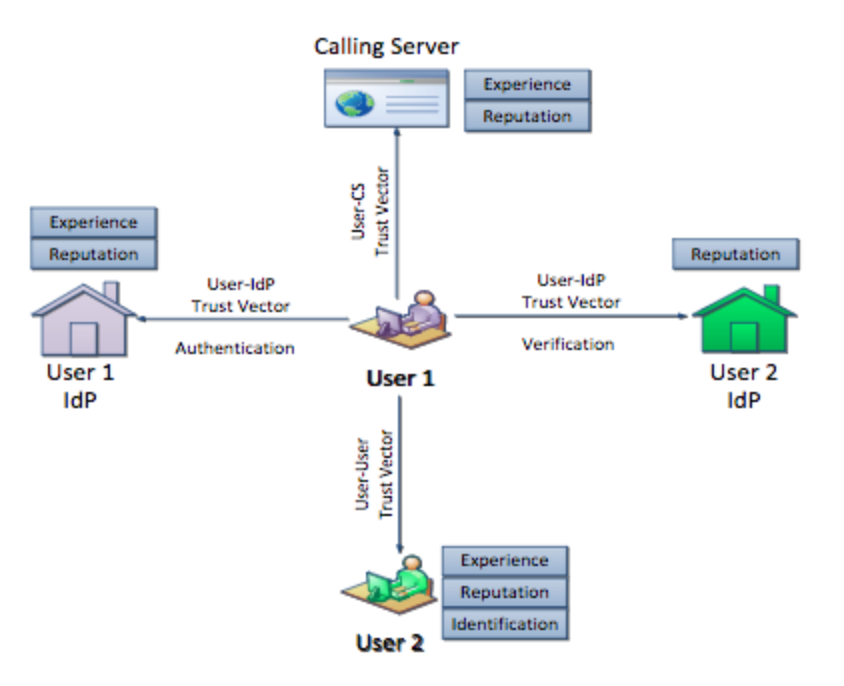
\includegraphics[scale=.8]{images/javed}
\end{center}
\caption{Javed \etal\cite{javed2016br2br} WebRTC trust model.}
\label{fig:javed}
\end{figure}

Copeland and Copeland proposed in 2016~\cite{copeland1question} a ``better than best effort'' architecture allowing communication services to select the appropriate network depending on selected profiles.
These profiles are built on balance between four considered criteria: QoS, Urgency, Security, and Affordability (QUSA).
Profiles and the associated network are selected based on the context of the communication. 
The context is derived from input from multiple sources, \eg calendar, social network, or location, with each source being attributed precision, accuracy, and confidence scores.
The overall architecture is summarised in Figure~\ref{fig:qusa}. 
The paper claims to have simulated 200 cases but point at the absence of real-world data.

\begin{figure}
\begin{center}
    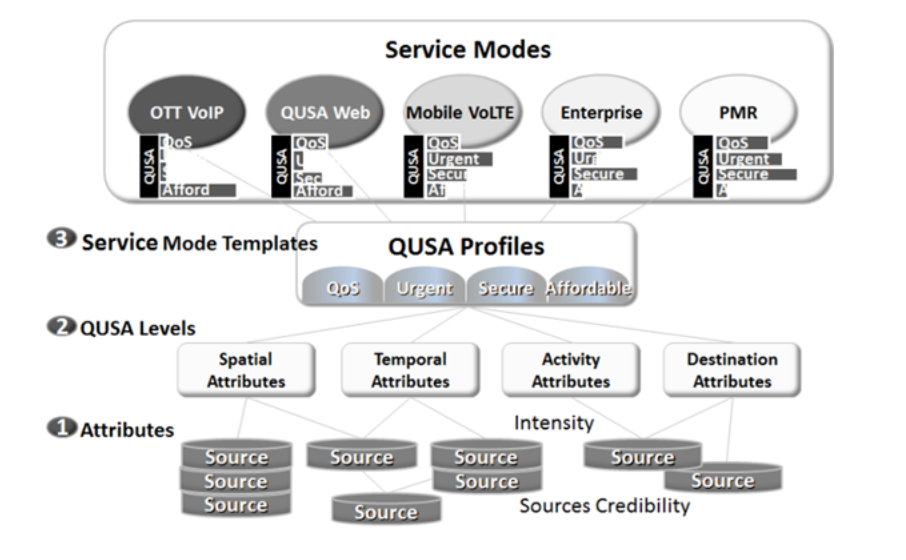
\includegraphics[scale=.8]{images/qusa}
\end{center}
\caption{Service Mode decision process based on context and QUSA profiles.}
\label{fig:qusa}
\end{figure}

\subsubsection{Social Threats (1)}
Following on their WebRTC trust model, Javed~\etal\cite{javed2017trustcall} propose a trust model evaluating trust in peers of a WebRTC communication in real-time.
In their model, a trust value is centrally computed by the communication service for each peer. 
This trust value is the weighted sum of an authenticity score, in fact a reputation, and a behavioural score based on talk time, incoming call numbers, and outgoing call numbers.
They simulate their approach and compare it to other trust models from the literature against some \gls{voip} social threats and trust model attacks.
Security considerations in this work are quite limited and only consider the authenticity of the other peer.
Furthermore, this authenticity of a peer is actually a reputation score rather than a measure of actual authentication.

In 2015, Vapen et al.~\cite{DBLP:conf/sec/VapenCMS15} studied the identity management landscape on the web\footnote{This paper is not part of our \gls{voip} security research collection.}. In their study, they classified the type of information shared by \gls{idp} to \gls{rp} in five classes: basic information, personal information, created content, friend's data, and a transversal action class.
They also defined semi-ordered risk types classes, build as conjunction of information shared classes. 
These classes range from R- to RA++ risk levels, A denoting action authorization.
In addition, their observations show that in practice \gls{rp} offer few choices of \gls{idp} to their users, with \SI{47}{\percent} offering only one \gls{idp}, and \SI{19}{\percent} offering four or more \gls{idp}. 
This situation profits to a few \gls{idp} trusting the top ranks, with Facebook as the number one, followed by Google and Twitter.

\subsubsection{Middleboxes (2)}
Johnston \etal\cite{johnston2013taking} look at the issues of WebRTC communication services in enterprise networks, \ie the traversal of enterprise firewalls for WebRTC session negotiated over \gls{https}.
They first present an overview of the issue and identify that current approaches for session border control and enterprise policies are not applicable to WebRTC.
The reason is that contrary to traditional \gls{voip} application using \gls{sip}, WebRTC applications may not expose sessions information to firewalls.
Several possible solutions are then described and discussed.
Other issues, not related to security, are also discussed such as the interoperation of WebRTC technologies with existing \gls{voip} infrastructures.

Singh \etal\cite{singh2015enterprise} implemented a Google Chrome extension to apply enterprise policies to WebRTC calls without help from underlying web application.
The extension overloads the WebRTC \gls{api} to intercept calls, it can then inserts user's enterprise identity in signalling messages.
Rather than implementing an \gls{idp} offering an \gls{idp} Proxy, the extension relies on an enterprise public key infrastructure to sign and verify signalling message.
The extension also forces the use of an enterprise media relay, \ie a modified \gls{turn} server responsible for applying enterprise's policies.

%\centering
\begin{table*}
\begin{tabular}{{@{}rlllllll@{}}}%\toprule\toprule
  &\textbf{Category / Title} & \textbf{Year} &\rotatebox{90}{\textbf{Security}} & \rotatebox{90}{\textbf{Trust}}& \rotatebox{90}{\textbf{Privacy}}& \rotatebox{90}{\textbf{Negotiation}}& \rotatebox{90}{\textbf{\gls{idp} Proxy}}\\\midrule

&\textbf{Social Threats}\\
\small{\cite{javed2017trustcall}}&\pbox{11cm}{\small{\textit{TrustCall: A Trust Computation Model for Web Conversational Services}}} & 2017 & & $\checkmark$ & & &  $\checkmark$ \\
\small{\cite{DBLP:conf/sec/VapenCMS15}}&\pbox{11cm}{\small{\textit{Information Sharing and User Privacy in the Third-Party Identity Management
               Landscape}}} & 2015 & & & $\checkmark$ \\
\midrule

&\textbf{Traffic Attacks}\\
\small{\cite{di2015decision}}&\pbox{11cm}{\small{\textit{A Decision Theory Based Tool for Detection of Encrypted WebRTC Traffic}}} & 2015 &  $\checkmark$ \\
\small{\cite{mauro_revealing_2017}}&\pbox{11cm}{\small{\textit{Revealing Encrypted WebRTC Traffic via Machine Learning Tools}}} & 2015 &  $\checkmark$ \\ 
\midrule

&\textbf{Overviews and Surveys}\\
\small{\cite{jennings2013real}}&\pbox{11cm}{\small{\textit{Real-time Communications for the Web}~}} & 2013 & $\checkmark$  & & & &  $\checkmark$\\ 
\small{\cite{barnes2014browser}}&\pbox{11cm}{\small{\textit{Browser-to-Browser Security Assurances for WebRTC}}} & 2014 & $\checkmark$ & & & &  $\checkmark$\\ 
\small{\cite{loreto_real-time_2012}}&\pbox{11cm}{\small{\textit{Real-Time Communications in the Web: Issue, Achievements, and Ongoing Standardization Efforts}}} & 2012 & $\checkmark$ \\ 
\small{\cite{loreto_how_2017}}&\pbox{11cm}{\small{\textit{How Far Are We from WebRTC-1.0?}}} & 2017 & $\checkmark$  & & & &  $\checkmark$\\ 
\small{\cite{rahaman2015survey}}&\pbox{11cm}{\small{\textit{A Survey on Real-Time Communication for Web}}} & 2015 & $\checkmark$  & & & &  $\checkmark$\\ 
\small{\cite{amirante2013seamless}}&\pbox{11cm}{\small{\textit{On the Seamless Interaction Between WebRTC Browsers and SIP-based Conferencing Systems}}} & 2013 & $\checkmark$ \\ 
\small{\cite{de2013web}}&\pbox{11cm}{\small{\textit{D.1.1 Web-platform security guide }}}  & 2013 & \checkmark \\
\small{\cite{bos2014case}}&\pbox{11cm}{\small{\textit{D1.2 Case Study: Security Assessment of WebRTC }}}  & 2014 & \checkmark \\
\midrule

&\textbf{Field Studies and System/Protocol Analysis}\\
\small{\cite{reiter2017webrtc}}&\pbox{11cm}{\small{\textit{WebRTC: Your Privacy Is at Risk}}} & 2017 & $\checkmark$ & & $\checkmark$ & &  $\checkmark$  \\
\small{\cite{al2017one}}&\pbox{11cm}{\small{\textit{One Leak Will Sink a Ship: WebRTC IP Address Leaks}}} & 2017 & & & $\checkmark$ \\
\midrule

&\textbf{Authentication Protocols}\\
\small{\cite{de2016ensuring}}&\pbox{11cm}{\small{\textit{Ensuring Endpoint Authenticity in WebRTC Peer-to-Peer Communication}}} & 2016 & $\checkmark$ & & & R & $\checkmark$\\
\midrule

&\textbf{Architectures}\\
\small{\cite{muranyi2013identity}}&\pbox{11cm}{\small{\textit{Identity Management in WebRTC Domains}}} & 2013 & & $\checkmark$ \\
\small{\cite{li2014calling}}&\pbox{11cm}{\small{\textit{Who Is Calling Which Page on the Web?}}} & 2014 & & $\checkmark$ & & &  $\checkmark$\\
\small{\cite{beltran2014user}}&\pbox{11cm}{\small{\textit{User Identity for WebRTC Services: A matter of trust}}} & 2014 & & $\checkmark$& $\checkmark$ \\
\small{\cite{beltran2015unified}}&\pbox{11cm}{\small{\textit{Unified Communications as a Service and WebRTC: an Identity-Centric Perspective}}} & 2015 & & $\checkmark$ & & &  $\checkmark$ \\
\small{\cite{beltran2015identity}}&\pbox{11cm}{\small{\textit{Identity Management for Web Business Communications}}} & 2015 & & $\checkmark$ & & & $\checkmark$\\
\small{\cite{javed2016browser}}&\pbox{11cm}{\small{\textit{Browser-to-Browser authentication and trust relationships for WebRTC}}} & 2016 & & $\checkmark$ & $\checkmark$ & &  $\checkmark$\\
\small{\cite{javed2016br2br}}&\pbox{11cm}{\small{\textit{Br2Br: a Vector-Based Trust Framework for WebRTC Calling Services}}} & 2016 & L  & $\checkmark$ & & &  $\checkmark$\\
\small{\cite{copeland1question}}&\pbox{11cm}{\small{\textit{A Question of Quality - VoIP, WebRTC or VoLTE?}}} & 2016 & & & & $\checkmark$ &$\checkmark$ \\
\midrule

&\textbf{Middleboxes}\\
\small{\cite{johnston2013taking}}&\pbox{11cm}{\small{\textit{Taking on WebRTC in an Enterprise}}} & 2013 & & P\\
\small{\cite{singh2015enterprise}}&\pbox{11cm}{\small{\textit{Enterprise WebRTC Powered by Browser Extensions}}} & 2015 &  & P & & & L\\

  \bottomrule
  \hline
\end{tabular}
\caption[Reviewed WebRTC Papers]{List of reviewed WebRTC papers. Checkmarks indicate whether the papers look or address the issues of security, trust model, privacy, security parameters negotiation, and the WebRTC identity architecture. The letters stand for L: \textit{limited}, R: \textit{recommends}, and P: \textit{policy trust}.}
\label{tab:SOTAobservations}
\end{table*}

\subsection{Observations}
We now compare the surveyed state of the art on WebRTC security to our research questions.
These observations allow us to narrow the focus of our contributions presented in later chapters.

Threats against user's security in the context of real-time multimedia communications and mechanisms to protect against these have been well-studied.
WebRTC has been built on this foundation, and the state of the art on \gls{voip} security research continued to develop since then.
As WebRTC is not a full-stack solution, we observe that researches on WebRTC and on WebRTC security mainly focus on security at the endpoint, including privacy risks for the users, and the issues of WebRTC deployment in enterprises.
One novelty introduced by the WebRTC security architecture is the integration of third-party \gls{idp} into the communication setup through the \gls{idp} Proxy mechanism.
This specification attracted a lot of interest from the community: as presented in Table~\ref{tab:SOTAobservations} we observe that out of 22 WebRTC security papers, a total of 13 papers reference the WebRTC identity architecture.
However, the security and privacy of this specification are only studied from a theoretical point of view~\cite{de2016ensuring}.
In particular, while WebRTC is intended to be interoperable with any \gls{sso} protocol, cross-implementation issues between the \gls{sso} protocol and WebRTC are rarely considered~\cite{li2014calling,de2016ensuring}.
The specification itself only sketches a short example using OAuth in annexe A~\cite{I-D.ietf-rtcweb-security-arch}. 
Additionally, other works study the privacy implications of the identity architecture but only consider the privacy threats posed by a malicious signalling server against user identity.
Consideration for this type of threats is already present in the WebRTC security architecture draft~\cite{I-D.ietf-rtcweb-security-arch}.
However, we do not observe research considering the privacy of the communication against the identity provider itself.

Besides understanding the threats faced by WebRTC users, we also want to act on a WebRTC session to raise the trust and security level.
Some surveyed work propose to negotiate the configuration of a WebRTC or \gls{voip} communication setup in order to achieve a given security level.
The solution of Copeland and Copeland~\cite{copeland1question} focus on selecting an appropriate underlying network, \ie at the network access layer, which does not allow to manage upper layer parameters.
Alia~\etal\cite{alia2010putting} propose an interesting model for balancing security and \gls{qos}.
However, their utility function is not convincing.
While an additive approach is coherent for modelling performance overheads, it does not achieve to model the dependent nature of security parameters.
For instance, a weak integrity on the signal path may have an important impact on confidentiality of the media path.

Increasing privacy, for instance to mitigate \gls{ice} \gls{ip} address leaks~\cite{al2017one}, mostly relies on permanent configuration options such as the selected \gls{os} or browser parameters.
Choosing proper actors to participate in the communication setup may also be a way to increase privacy, either because they implement privacy-preserving protocols or because they are trusted to not compromise user's privacy.
Regarding this last point, we note that De~Groef~\etal\cite{de2016ensuring} recommend that browsers allow users to select an \gls{idp} of their choice, \ie trusted, to participate in WebRTC sessions set up.

We want a model representing both security and trust to help users in the configuration and negotiation of WebRTC security parameters.
A lot of work has been conducted on modelling reputational-trust in WebRTC~\cite{beltran2014user,beltran2015unified,beltran2015identity,javed2016browser,javed2017trustcall}.
However, these papers generally do not consider the security of the session and the strength of security parameters in their models.
At most, only the user authentication strength is taken into account~\cite{javed2016br2br}.
Alternatively, some researchers~\cite{johnston2013taking,singh2015enterprise} consider trust policies with respect to WebRTC security.
However, they focus on applying enterprise policies and do not propose a complete model of WebRTC security.

\clearpage
\invisiblesection{Summary}
\label{sec:sotaSummary}
%\vspace*{3cm}

\blockmargin%
%\hspace{-\marginparwidth}\hspace{-\marginparsep}
\makebox[\overflowingheadlen][l]{
\begin{minipage}{\overflowingheadlen}

\begin{mdframed}[style=SOTAFrame,frametitle={\ref{sec:sotaSummary}~Summary}]

We conducted a research survey on \gls{voip} and WebRTC security research.
In total, we classified 208 research papers of which 23 were actually addressing WebRTC security. 
We then reported on the researches conducted in these 23 WebRTC security paper.

\medskip

Firstly, we observe that the WebRTC identity architecture attracted a lot of interest from the community.
However, we note that the security and privacy of the specification are only studied from a theoretical point of view~\cite{de2016ensuring}. 
In particular, the cross-implementation issues between \gls{sso} protocol and WebRTC are rarely considered~\cite{li2014calling,de2016ensuring}. 
The specification itself only sketches an implementation with the OAuth protocol in its annexe~\cite{I-D.ietf-rtcweb-security-arch}. 
We neither observe research considering the \gls{idp} as a possible attacker of the user's privacy.
In order to remedy to this issue, we intend to base our analysis of the WebRTC security and identity architecture on an actual implementation of \gls{sso} protocols in the context of a WebRTC service.

\medskip

Secondly, one of our research objectives is to build a model representing the trust and security of a WebRTC session and capable of returning a single metric.
In our survey, however, we do not observe research combining elements of trust and security models.
At best, one of the trust model uses limited security parameters~\cite{javed2016br2br} which confirms that combining trust and security for \gls{voip} is a novel approach.
Existing researchs work on the dynamic configuration of \gls{voip} services, but also uses a simplistic security model~\cite{alia2010putting}.
Nevertheless, other researchers recommend that users be given more control over which \gls{idp} they use in \gls{voip}~\cite{de2016ensuring} and more broadly on the Web~\cite{Sun2011}.
As we want to give them more control over the trust and security of their WebRTC session, we will focus on allowing users to negotiate WebRTC identity parameters. 

\end{mdframed}

\end{minipage}
}
\unblockmargin





%      \newgeometry{
%            left=2.2cm,
%            right=2.2cm,
%            top=2.2cm,
%            bottom=3.5cm,
%            ignoremp}
%      %\printbibliography
%      
%      \printbibliography[title={WebRTC Security State of the Art},keyword=sota]
%      
%      \clearpage
%      
%      
%    \restoregeometry

\newpage

    \newgeometry{
            left=2.2cm,
            right=2.2cm,
            top=2.2cm,
            bottom=3.5cm,
            ignoremp}
            
\renewpagestyle{scrheadings}{
  {\makebox[2em][r]{\thepage}\quad\rule{1pt}{100pt}\quad\leftmark}%
  {\hfill\rightmark\quad\rule{1pt}{100pt}\quad\makebox[2em][l]{\thepage}}%
  {}
}{
  {}%
  {}%
  {}
}
\renewpagestyle{plain.scrheadings}{
  {}%
  {}%
  {}
}{
  {\thepage}%
  {\hfill\thepage}%
  {}
}
            
\part{Contributions}
\label{contributions}

\restoregeometry
\renewpagestyle{scrheadings}{
  {\hspace{-\marginparwidth}\hspace{-\marginparsep}\makebox[\overflowingheadlen][l]{\makebox[2em][r]{\thepage}\quad\rule{1pt}{100pt}\quad{}\leftmark}}%
  {\makebox[\overflowingheadlen][r]{\rightmark\quad\rule{1pt}{100pt}\quad\makebox[2em][l]{\thepage}}}%
  {}
}{
  {}%
  {}%
  {}
}
\renewpagestyle{plain.scrheadings}{
  {}%
  {}%
  {}
}{
  {\thepage}%
  {\makebox[\overflowingheadlen][r]{\thepage}}%
  {}
}

\chapter*{Foreword on Methodology}
\thispagestyle{empty}
\addcontentsline{toc}{chapter}{Foreword on Methodology}

As we explained in Section~\ref{sec:webrtc}, WebRTC is a set of standard specifications aiming to provide to webpages the capability to setup \gls{voip} communications.
These specifications also rely on other standards and techniques: authentication delegation protocols, \gls{voip} protocols and archirectures, JavaScript \gls{api}, cryptography, ...
At the heart of the WebRTC identity architecture is the proposal of an abstract authentication interface for peer-to-peer authentication and the claim that trust in an \gls{idp} can replace trust in the signalling path. 
We aim to study these propositions and at the same time answer our research questions.
However, we believe that formal paper-based study of standards must be conducted in conjunction with study of running implementations, in a complementary approach.
Indeed, standards are ultimately implemented in actual running code.
During this continuous process, implementors may take liberties with the specification, add non-standard functionalities, or decide to not implement some of them.
Furthermore, cross-implementation issues may arise, in particular when the integration of two specifications has not been thoroughly considered.
This is precisely the case of the WebRTC identity architecture which only sketches the OAuth~2 protocol integration.
It appears that, from our state of the art survey in Chapter~\ref{sota}, most of the researches on WebRTC security have been conducted without considering actual implementations.

\begin{figure}[H]
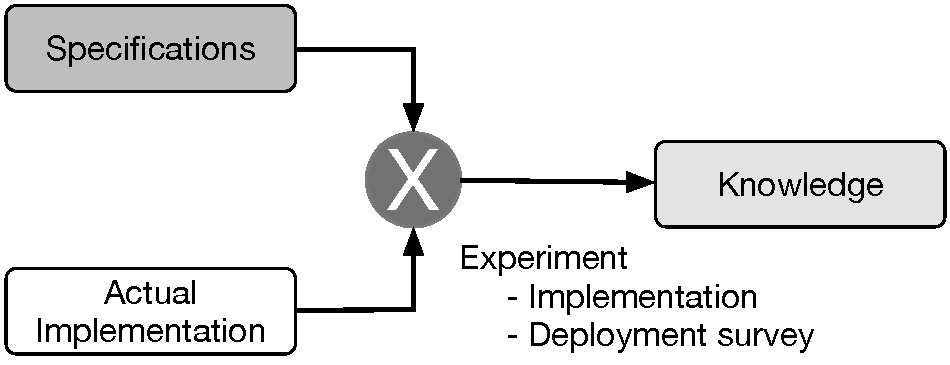
\includegraphics[scale=.5]{images/science}
\caption{Overview of our Scientific Methodology}
\label{science}
\end{figure}

Our approach, which we schematise in Figure~\ref{science}, differs.
The first step of our work is to conduct a study of these standards and techniques.
We presented the results of this step in Chapter~\ref{security}~and~\ref{sota}.
However, we then use actual implementations to answer our research questions. 
To do so, we conduct two types of experiments:
\begin{itemize}
\item In implementation experiments we develop software to put an already specified or a new functionality into action.
This allows us to discover actual issues encountered during the implementation and integration processes.
We describe our implementations so that our experiments can be reproduced~\footnote{The description of our implementations may also be helpful for developers facing similar needs.}.
\item In deployment survey experiments, we observe whether a functionality is implemented or used in existing and deployed softwares.
Observing an exposed functionality demonstrates if and how it can be used, while observing its actual usage reveals its importance for other services.
\end{itemize}

These experiments form the basis of our scientific methodology which we apply in the following contribution chapters.



\chapter{Privacy Implications of the WebRTC Identity Architecture}
\label{webrtcprivacy}
\begin{quote}
\textit{
A claim of the WebRTC security architecture specification~\cite{I-D.ietf-rtcweb-security-arch} is that trust in the signalling layer can be replaced by trust in the \gls{idp}.
This has implications regarding potential privacy issues.
As signalling and identity functions are decoupled, a new actor (the \gls{idp}) is introduced in the communication setup.
Even-though \gls{idp} already occupy a central role on the Web, their role in WebRTC has the potential to reinforce their position.
In this chapter, we study the privacy implications of the WebRTC Identity Architecture.
This part of the WebRTC specification lacks support on web browsers.
To the best of our knowledge, there is no publicly implementation or deployment of a WebRTC identity enabled WebRTC service or of an \gls{idp} supporting the WebRTC identity architecture.
To better understand the WebRTC Identity Architecture, it is thus necessary to first implement it.
We describe our implementations in Section~\ref{idpproxyimplem}.
We then detail additional privacy considerations in Section~\ref{sec:privacyissue}.
One issue we observe is that the \gls{idp} choice is limited by the \gls{cs} which may appear contradictory with the initial objective of the specification.
In Section~\ref{userschooseidp} we study why users cannot choose their \gls{idp} on the Web. 
}
\end{quote}

\begin{figure}[H]
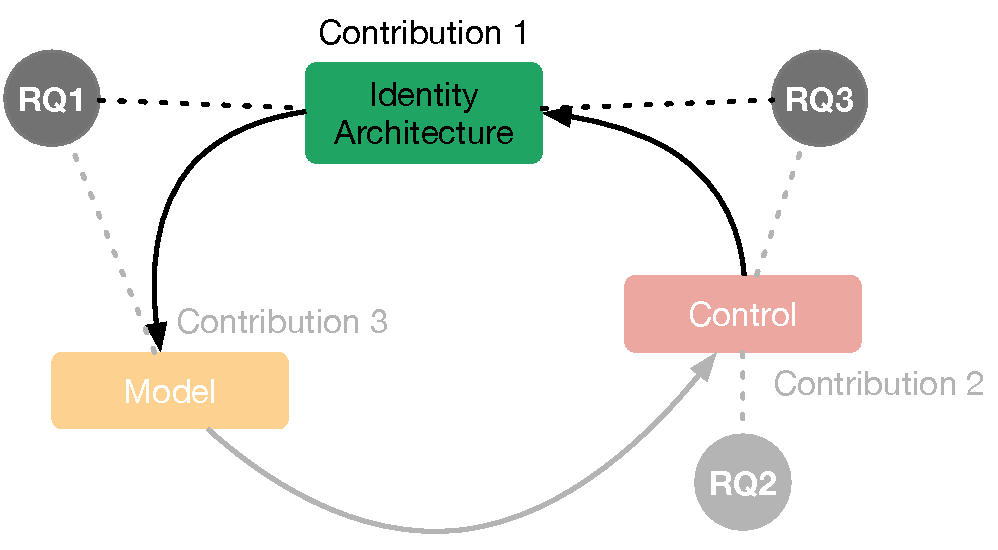
\includegraphics[scale=.5]{images/contrib1}
\caption{Overview of our Contributions: Study of the WebRTC Identity Architecture.}
\label{contrib1}
\end{figure}


\glsresetall
\section{WebRTC Identity Architecture Implementation}
\label{idpproxyimplem}
The explicit peer authentication proposed by the WebRTC specification plays a central part of the WebRTC identity architecture.
But it is also, for the moment, a feature whose implementation in browser lags behind others WebRTC features.
The \texttt{RTCPeerConnection} identity interface is only implemented in Firefox.
As a result and to the best of our knowledge, no \gls{idp} or WebRTC service are supporting it\footnote{\url{https://bugs.chromium.org/p/chromium/issues/detail?id=493640}}.
Our first research question (RQ1) consists in understanding the risk for the user of a WebRTC session. 
More particularly, in this section we address the following question:
\begin{itemize}
\item \textbf{RQ1.1}: Are there any security vulnerabilities in the identity path of the WebRTC security architecture?
\end{itemize}
We want to validate our work on a running implementation of the WebRTC identity architecture.
To do so, we develop a simple WebRTC service\footnote{\url{https://github.com/Sparika/ACOR\_SDP}} offering communication for two users in a single room.
The communication server is built with the NodeJS framework.
Session signalling is done through the \gls{cs} server over web sockets and the JavaScripts client code manages the call session.
We conduct our tests on Firefox version 50.1.0. 

As the RTCPeerConnection identity interface is provided by Firefox, the missing part of the WebRTC identity architecture is an \gls{idp} exposing \gls{idp} Proxy.
In addition to a WebRTC service, we also implement \gls{idp} Proxies for three different \gls{idp}, following the WebRTC specification.
The first \gls{idp} is actually our WebRTC communication service itself in what we call a local authentication scenario.
We present this implementation in Section~\ref{sec:idpstd}.
Our two other \gls{idp} Proxies are developed for two OIDC servers.
The first server is one of the reference implementations by Nat Sakimura\footnote{\url{https://github.com/reTHINK-project/dev-IdPServer-phpOIDC}}, while the second one is an implementation in NodeJS\footnote{\url{https://github.com/reTHINK-project/dev-IdPServer}}.
We also conducted these implementations within the context of the reThink project, in order to reuse WebRTC identity architecture for the reThink Identity Module (see Section~\ref{sec:rethink}).
Section~\ref{sec:idpoidc} details how we implement \gls{oidc} \gls{idp} Proxies and how we adapt their respective \gls{idp} servers.
Finally, in Section~\ref{sec:proxyImplemObs} we discuss our implementations.

\subsection{Local Authentication Implementation}
\label{sec:idpstd}
\marginpar{
\captionsetup{type=figure}
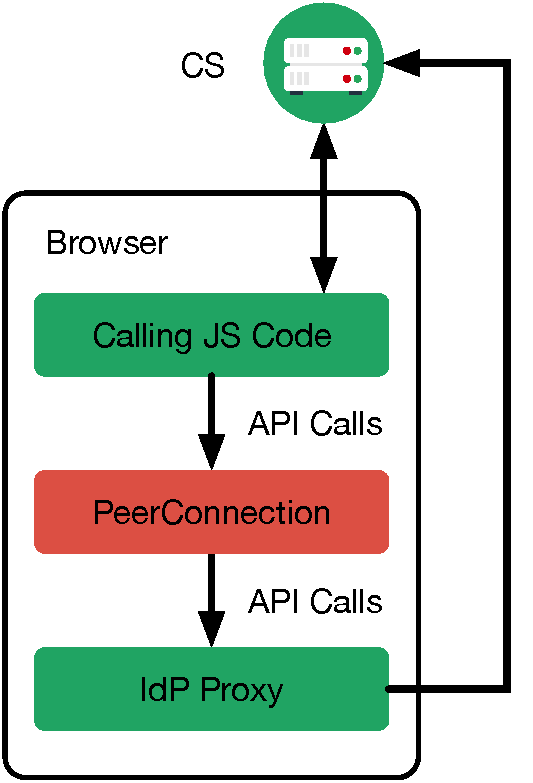
\includegraphics[width=\marginparwidth]{images/localAuthArch}
\caption{Local Authentication Architecture}
\label{fig:localAutharch}
}
Local authentication refers to a scenario where the \gls{cs} also plays the role of the \gls{idp} in the WebRTC identity architecture, as in Figure~\ref{fig:localAutharch}.
It is not the architecture initially envisioned by the specification.
As we explained in Section~\ref{sec:webrtcid}, the decoupling of identity and signalling functions are meant to prevent the \gls{cs} from setting up a man-in-the-middle during the call session establishment.
This architecture may nonetheless be useful.
Firstly, it provides a simple test use case for an \gls{idp} Proxy with a login and password authentication as used by most websites not relying on \gls{idp}.
Secondly, in an interoperable signalling architecture, multiple \gls{cs} are used to establish the session.
A user may not trust the signalling path, except for his own \gls{cs}. 
In this case using his \gls{cs} as an \gls{idp} would offer a protection against man-in-the-middle attack from other \gls{cs}.
Finally, in compatibility scenarios call transit through a legacy interface, for instance, a \gls{sip} Gateway.
In this case, the legacy interface plays the role of both the \gls{cs} and the \gls{idp}.

Functionally, our implementation of the \gls{idp} Proxy maps the identity assertion to the \texttt{contents} parameter, \ie the session fingerprint.
The identity assertion thus serves as the key to retrieve claims covered by the assertion, and verify in the process that these claims were effectively registered on the \gls{idp}.
Figure~\ref{localAuthGen} presents the identity assertion generation interface exposed by the server to the \gls{idp} Proxy and its sequence diagram.
To store a new pair, the \texttt{generateAssertion} function of the \gls{idp} Proxy POST a content to the \texttt{/assertion} REST interface. 
After the server checked that the user is logged in, the user's identity and content parameter are stored in a map and the key is returned with an \gls{http} 200 success response.
The \gls{idp} Proxy then uses the key to instantiate an \texttt{RTCIdentityAssertionResult} (see Figure~\ref{idAssertWebIDL}) and resolve the \texttt{generateAssertion} promise with it.
On the promise's resolution, the browser adds the assertion dictionary to the \gls{sdp} message.

\begin{figure}[H]
\begin{Verbatim}[commandchars=\\\{\}]
dictionary \textcolor{matred}{RTCIdentityAssertionResult} \{
    required \textcolor{matred}{RTCIdentityProviderDetails}       idp;
    required \textcolor{matblue}{DOMString    }        assertion;
\};

dictionary \textcolor{matred}{RTCIdentityProviderDetails} \{
    required \textcolor{matblue}{DOMString    }                domain;
             \textcolor{matblue}{DOMString}                        protocol = "default";
\};

\end{Verbatim}
\caption[RTCIdentityAssertionResult specification in WebIDL]{RTCIdentityAssertionResult specification in WebIDL. The assertion is an "opaque string that MUST contain all information necessary to assert identity". It is consumed by the validating IdP.}
\label{idAssertWebIDL}
\end{figure}

Alternatively, if the user does not have an active session, the \texttt{generateAssertion} promise is rejected with an \texttt{IdPLoginError} \gls{json} object.
This object may contain an \texttt{idpLoginUrl} element, which can be used by the client service to open a login page on the \gls{idp}.
A successful login following this \gls{url} is signalled by a \texttt{LOGINDONE} message sent using the postMessage \gls{api} to the login page's opener window, \ie the communication service client page.

\begin{Verbatim}[commandchars=\\\{\}]
<script>window.opener.postMessage(\textcolor{matblue}{'LOGINDONE'}, \textcolor{matblue}{'*'})</script>
\end{Verbatim}

Figure~\ref{localAuthVerif} shows the \textit{local} identity assertion validation REST interface and its associated sequence diagram.
To validate a received identity assertion, the peer's browser downloads the \gls{idp} Proxy from the \gls{idp} which produced the identity assertion.
The \texttt{RTCIdentityProviderDetails} dictionary (see Figure~\ref{idAssertWebIDL}), included in the assertion, describes the \gls{idp} Proxy location.
Once the browser instantiated the verifying \gls{idp} Proxy, it calls the \gls{idp} Proxy's \texttt{validateAssertion} function.
Our implementation of this function sends a GET request to the \texttt{/assertion} interface, using the provided assertion (see Figure~\ref{idpproxyimplem:getapi}). 
The result of the request is a \gls{json} object containing the stored identity and content.
This object is used to instantiate an \texttt{RTCIdentityValidationResult} dictionary (see Figure~\ref{idValidWebIDL}) which is then returned to the browser.
The browser verifies that the provided \texttt{contents} matches the \gls{sdp} fingerprint attribute, binding the fingerprint to the assertion's \texttt{identity}.

\begin{figure}[H]
\begin{Verbatim}[commandchars=\\\{\}]
dictionary \textcolor{matred}{RTCIdentityValidationResult} \{
    required \textcolor{matblue}{DOMString    }                identity;
    required \textcolor{matblue}{DOMString    }                contents;
\};

\end{Verbatim}
\caption{RTCIdentityValidationResult specification in WebIDL.}
\label{idValidWebIDL}
\end{figure}

\begin{figure*}
\begin{subfigure}{\textwidth}
\begin{center}
    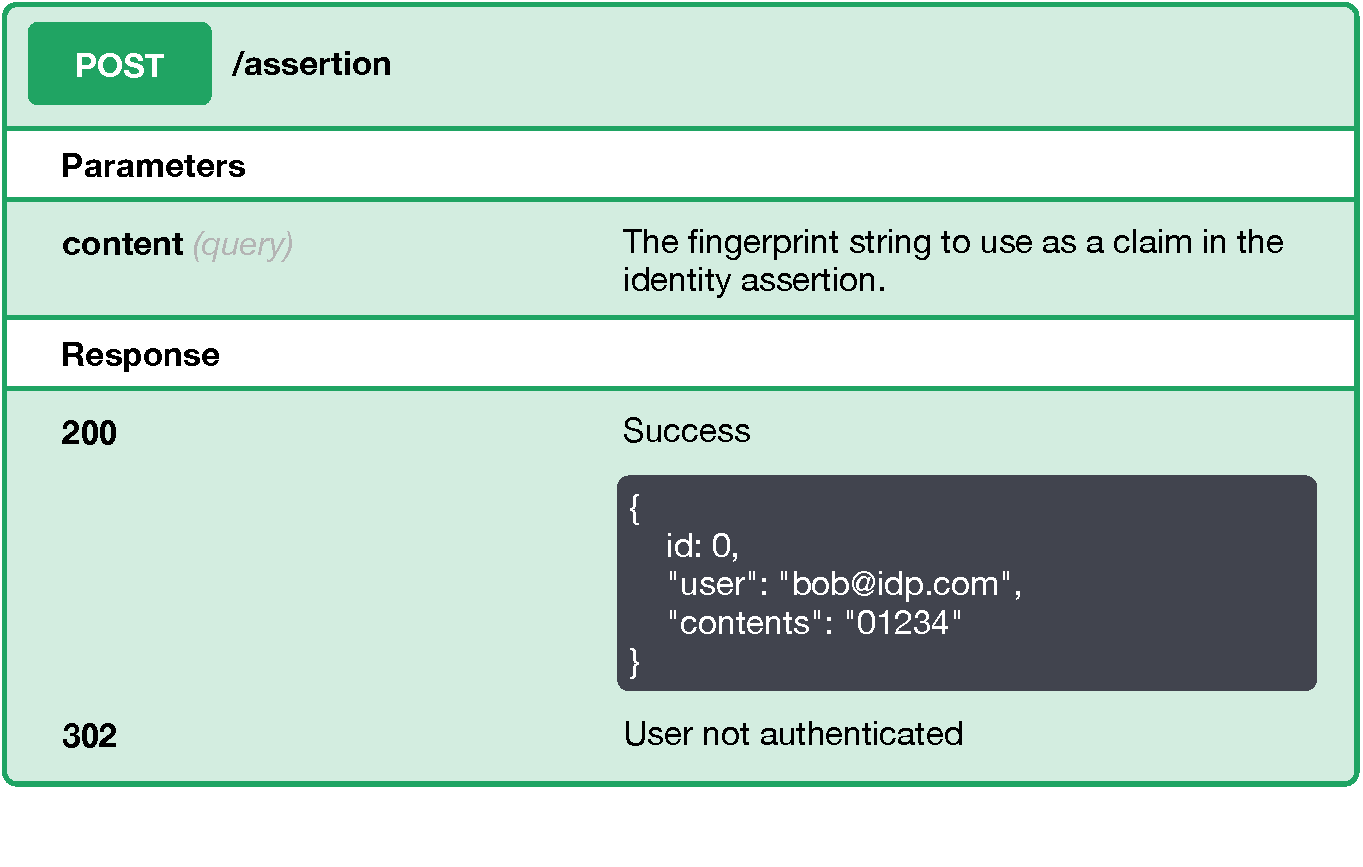
\includegraphics[scale=0.5]{images/localProxyAPIPOST}
\caption{/assertion POST API}
\label{idpproxyimplem:postapi}
\end{center}
\end{subfigure}
\begin{subfigure}{\textwidth}
\begin{center}
    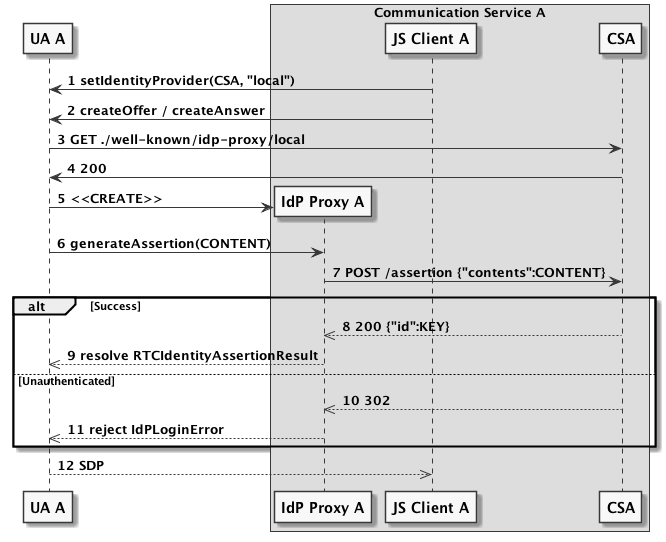
\includegraphics[scale=0.55]{images/localAuthGen}
\caption{Sequence Diagram}
\label{localAuthGen:seq}
\end{center}
\end{subfigure}
\caption{Local Identity Assertion Generation}
\label{localAuthGen}
\end{figure*}

\begin{figure*}[tbp]
\begin{subfigure}{\textwidth}
\begin{center}
    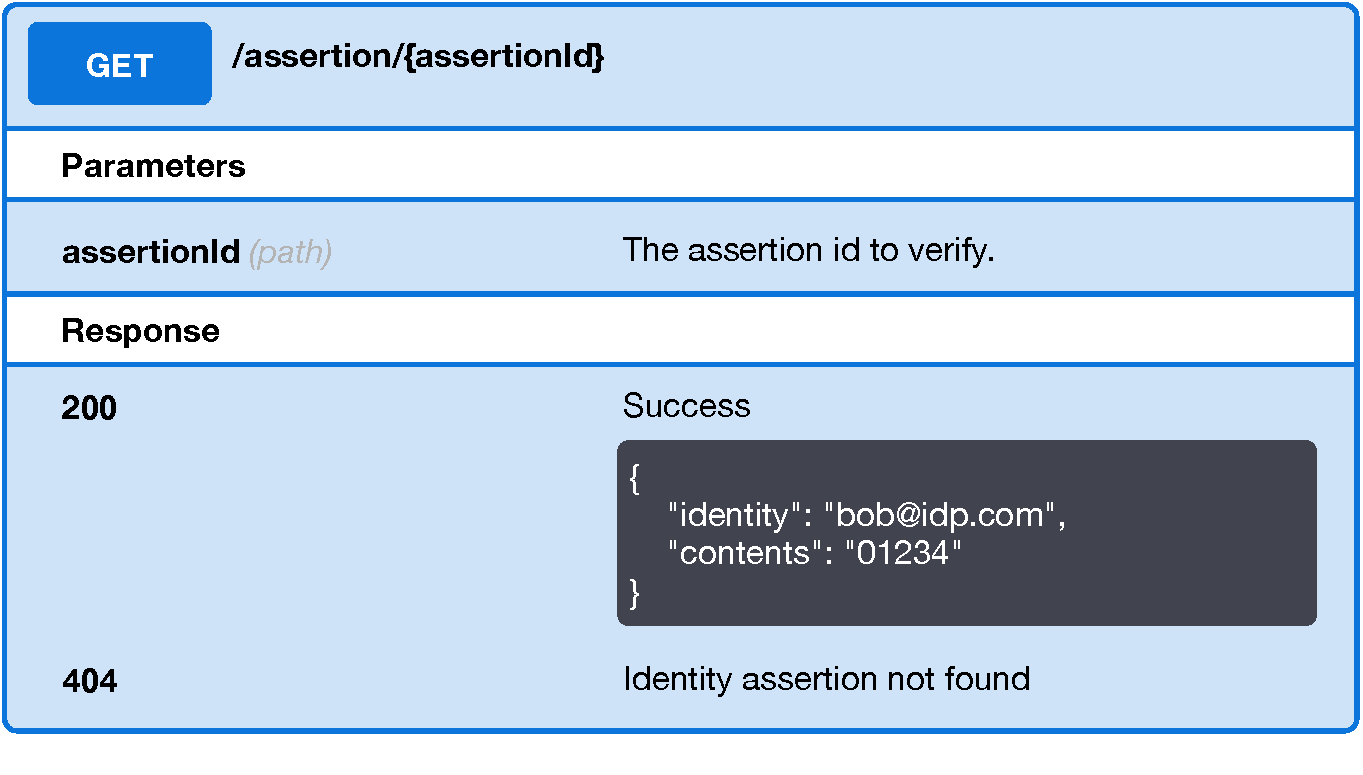
\includegraphics[scale=0.5]{images/localProxyAPIGET}
\caption{/assertion GET API}
\label{idpproxyimplem:getapi}
\end{center}
\end{subfigure}

\begin{subfigure}{\overflowingheadlen}
\centering
    \includegraphics[scale=0.55]{images/localAuthVerif}
\caption{Sequence Diagram}
\label{localAuthVerif:seq}
\end{subfigure}
\caption{Local Identity Assertion Verification}
\label{localAuthVerif}
\end{figure*}


\subsection{IdP Proxy with OpenID Connect}
\label{sec:idpoidc}

In order to integrate our \gls{oidc} servers into the WebRTC identity architecture, the \gls{idp} Proxy acts as the \gls{oidc} client.
In this role, the \gls{idp} Proxy requests an ID Token to the \gls{idp}.
The \gls{idp} authenticates the user and verifies that the user has authorized the \gls{idp} Proxy to obtain an ID Token.
As the \gls{idp} Proxy is a JavaScript code running inside the user's browser, \ie client side rather than server side, we use the \gls{oidc} \textit{implicit flow}.
This flow allows the client to directly get the requested token, as explained in \ref{sec:authProtocol}.
The resulting ID Token covers the user's identity and the session fingerprint as claims.
It thus serves as the WebRTC identity assertion.
Our implementation, however, requires additional modifications to \gls{oidc} requests.

Firstly, we include the session fingerprint as a claim of the ID Token payload so that it is covered by the server's signature.
To send it to the server, we define a new request parameter, \texttt{rtcsdp}, to convey this value in the request.
In practice, this parameter function is quite similar to the \texttt{nonce} request parameter.
Both convey random opaque numbers making the request unique.
However, in some cases, a WebRTC session may reuse a previously established key and thus the same session fingerprint twice.

Secondly, \gls{oidc} interactions with the user normally happen through a new tab or popup opened by the browser.
This graphical user interface allows the \gls{idp} to authenticate the user or request user's consent before authorizing the requesting client.
However, in our case, the \gls{idp} Proxy is running in a sandboxed invisible iframe.
The \gls{oidc} \texttt{/authorize} GET request (see Figure~\ref{idproxyimplem:oidcrequest}) is thus executed through the Fetch \gls{api}\footnote{Fetch is a standard web \gls{api} for network requests similar to the XMLHttpRequest (XHR) interface. An advantage of using the Fetch \gls{api} is that it easily integrates with the promise based WebRTC interfaces. See \url{https://developer.mozilla.org/en/docs/Web/API/Fetch\_API} for more details.}.
Such requests are invisible to the users, no new tab or window are opened.
Hence why the \gls{idp} Proxy has to throw an \texttt{IdPLoginError} in order to interact with the user.
As we described in Section~\ref{sec:idpstd}, this happens if the user is unauthenticated.
In the \gls{oidc} case, it also happens if the \gls{idp} Proxy client has not been authorized by the user.
The login or authorization URL is returned in an \texttt{IdPLoginError} to the \gls{cs}, which opens it so that the user can login or authorize the \gls{idp} Proxy.
In either case, the process followed by the user lands on a page messaging the \texttt{LOGINDONE} signal to the \gls{cs}.
The url of this page is defined using the \texttt{redirect\_uri} parameter of the \texttt{/authorize} request.
When receiving this message, the \gls{cs} restarts the \texttt{generateAssertion} procedure.

Finally, we also implement a new \texttt{response\_mode} value.
In the \gls{oidc} implicit flow, a successful authorization redirects to the client web page.
The ID token would be returned with the redirection either in the redirected URL's query or fragment.
However, both query or fragment are inaccessible from a Fetch (or XHR) response after following a redirection. 
Instead, the \gls{idp} returns the ID Token in the response body.
We thus define a new \texttt{response\_mode} value: \texttt{body} and modify the \gls{idp} server implementation accordingly.

Note that the \texttt{response\_mode} and \texttt{redirect\_uri} parameters are conflicting as they correspond to different HTTP response code, 200 and 302 respectively.
In our implementation, the \texttt{redirect\_uri} is only followed if \texttt{response\_mode} is not set to \texttt{body}.
Figure~\ref{idproxyimplem:oidcrequest} shows our modified \texttt{/authorize} request specification.

\begin{figure*}[tbp]
\begin{subfigure}{\textwidth}
\centering
    \includegraphics[scale=0.5]{images/OIDCProxyAPI}
\caption{/authorize GET API}
\end{subfigure}

\begin{subfigure}{\overflowingheadlen}
\centering
    \includegraphics[scale=0.55]{images/oidcAuthGen}
\caption{Sequence Diagram}
\end{subfigure}
\caption{OIDC Assertion Generation}
\label{idproxyimplem:oidcrequest}
\end{figure*}

To verify the ID Token validity, its signature must be verified by the \gls{idp} Proxy when it is executed from the other peer's browser.
It is either possible to add the \gls{idp}'s public key in the \gls{idp} Proxy code or retrieve it from a secured location on the \gls{idp}.
Optionally a reference to the key \gls{url} could be included in the ID Token header \texttt{jku} parameter.
This solution is discouraged by the \gls{oidc} specification which states that ``ID Tokens SHOULD NOT use the JWS or JWE x5u, x5c, jku, or jwk Header Parameter fields''~\cite{sakimura_openid_2014}.


\subsection{Observations}
\label{sec:proxyImplemObs}
We note that the Firefox implementation is more restrictive than the specification regarding identity format.
Firefox requires that the identity, the human-readable identifier, be in an email format with the domain of the email equals to the \gls{idp} Proxy domain.
This format prevents domains from asserting identity from other domains, \eg identifier ending in \url{@orange.com} could not be claimed by an \gls{idp} Proxy from the \url{dr.evil.net} domain.
However, using the email's domain as an indication of the \gls{idp}'s domain name is often an over-simplification.
As an example, Figure~\ref{fig:googleIdSelector} shows the Google identity selection popup.
Although the popup's domain name, \ie Google's \gls{idp} domain, is \url{accounts.google.com}, user's identifiers may end in \url{@gmail.com}.
Some valid identifiers may even end in other domain names if the user did not activate his Gmail mailbox, for example, \url{@orange.com}.

As shown by Table~\ref{tab:localProxyLines} the implementation of the local \gls{idp} Proxy is quite simple.
Proxy, Routes, and Model give the new and total number of JavaScript code lines respectively for the \gls{idp} Proxy, the \gls{http} interface implementation, and the database model.
On the project as a whole, our implementation required only 120 JavaScript code lines.
A number to be compared to the 6641 code lines, excluding NodeJS dependencies, of the full WebRTC service project.

\begin{table}
\begin{tabular}{{@{}lll@{}}}\toprule\toprule
  \textbf{Module} & \textbf{New code lines} & \textbf{Total code lines} \\\midrule
  \textbf{Proxy} & 66 & 66\\
  \textbf{Routes} & 38 & 290\\ 
  \textbf{Model} & 16 & 89\\\midrule
  \textbf{Project} & 120 & 6641\\\bottomrule
  \hline
\end{tabular}
\caption[JS code lines for local IdP Proxy]{JavaScript code lines for the local authentication IdP Proxy implementation.}
\label{tab:localProxyLines}
\end{table}

Compared to the local \gls{idp} Proxy, implementation of an \gls{oidc} \gls{idp} Proxy is a complex task.
Firstly, while following the same structure, the \gls{idp} Proxy is larger due to its requirement of ID Token signature verification, client key retrieval, and the handling of \gls{json} objects.
The \gls{idp} Proxy JavaScript file contains 207 JavaScript code lines.
The more complex modifications are however made on the \gls{oidc} server itself.
We add a few utility functions to the \gls{http} interface, but we also modify the core \gls{oidc} modules to support the parameters we introduced: \texttt{response\_mode=body} and the \texttt{rtcsdp} ID Token claim.
While these modifications are not that heavy in terms of code lines, they require the understanding and modification of a large code base.
As an example, the NodeJS dependency implementing the \gls{oidc} specification contains 1274 code lines in a single file.

Another issue of the \gls{oidc} implementation is its reliance on non-standard modification of the specification.
Industrial deployment of standards protocols may follow strict policies regarding the implementation of non-standard features.
In our case and due to the policies of our company, integrating our proposed change to the \gls{oidc} server in production would have required to first get them published by the OpenID foundation. 
The complexity of the \gls{oidc} implementation does not seem to brings benefits compared to the simple solution of the local authentication \gls{idp} Proxy.

Our implementations shows that \gls{oidc} facilitates the creation and signature of WebRTC identity assertion in an open standard format: \gls{oidc} ID Token.
However, it requires the modification of a complex code base not initially designed for this use case.
While using the ID Token format may have practical use cases to exchange WebRTC Identity assertion.
For some use cases, it may be as simple to use a map interface secured through \gls{https}.

\begin{figure}[h]
\includegraphics[width=1.3\marginparwidth]{images/googleIdSelector}
\caption[Google Identity Selection Page]{Google identity selection webpage.}
\label{fig:googleIdSelector}
\end{figure}

\section{RQ1.1 Additional Privacy Considerations}
\label{sec:privacyissue}

We presented the WebRTC security architecture in Section~\ref{sec:websecurity} and reviewed previous research works on WebRTC security in Section~\ref{sec:sota2012+}.
From this work, we observed that the identity path proposed by WebRTC security architecture has only been studied from a theoretical point of view and that in these works \gls{idp} had not been considered as possible attackers against the users' privacy.
In this section, we answer RQ1.1 by presenting new risks for the user's privacy introduced by the \gls{idp} Proxy component.
These privacy considerations were revealed by our implementation process.

\subsection{Audience Issue}
In addition to the \texttt{rtcsdp} claim, \ie the session fingerprint, the WebRTC identity assertion carries two important information: the peer's identity in human readable form, and the peer's identity provider fully qualified domain name.
Both pieces of information are necessary so that the assertion can be verified and associated with a peer's identity.
But from a privacy point of view, they are sensible identifying information.
In the \gls{sdp} message, the identity assertion is an opaque string encoded in base 64, which means that it has no actual definition.
However, the \gls{idp} Proxy can be downloaded by any party and instantiated to decode the identity assertion.

Although we explain this privacy issue with the \gls{oidc} scenario, it is present whether or not the \gls{idp} Proxy is based on \gls{oidc}.
As we explained in Section~\ref{sec:authProtocol}, OpenID Connect is based on OAuth2, an authorization protocol.
As such the concept of authorization and user consent is central to the protocol.
In theory, the client, identified by the \texttt{client\_id} in \gls{oidc} requests and the \texttt{audience} claim, is authenticated by the \gls{idp}.
In the implicit flow, the client authentication is not performed explicitly and instead relies on the \texttt{redirect\_uri} redirection to the client.
In the WebRTC use case of user-to-user authentication, the \texttt{redirect\_uri} is not followed as the ID Token is transmitted to the other peer over \gls{sdp} signalling.
There is no clear definition of the intended audience\footnote{The audience may not even be known a priori, for instance in the case of a call to an anonymous peer.} and in our implementation we define and use a unique \gls{idp} Proxy client and \texttt{client\_id}.
We explored the alternatives of one \texttt{client\_id} for each users, each \gls{cs}, or for each pair of user/\gls{cs} without finding clear advantage to any of these solutions.

As represented in Figure~\ref{idProxyWebIDL}, both \texttt{generateAssertion} and \texttt{validateAssertion} functions use an origin parameter.
This parameter is the origin of the \gls{cs} which required the instantiation of the \gls{idp} Proxy
However, the \texttt{validateAssertion} is executed after the identity assertion is transmitted over the signalling path.
As a result, the \gls{idp} does not know the signalling endpoint's origin during the generation of the assertion.
Some policy checks could still be applied during the execution of the \texttt{validateAssertion} function, eventually preventing the decoding and decryption of the identity assertion.
But the specification does not define the error that should be returned in this scenario and does not plan for transmitting a consent request back to the user.
Implementing such consent mechanism could be allowed using a push notification to the user's device.

On the other hand the \texttt{generateAssertion} can interact with the user through the \texttt{\gls{idp}LoginError}.
It can thus be subject to user authorization and \gls{idp} policies, as long as the \gls{idp} implements such mechanism.
Otherwise, without appropriate protection on the \gls{idp} Proxy, a web page could look for the user's identity.
This could reveal user identities, or at least existing user accounts on \gls{idp}s.
For instance, given a list of WebRTC compatible \gls{idp}s, running the script described in Figure~\ref{fig:audAttack} would reveal identity assertion from unprotected \gls{idp}s with active sessions.
This is a major issue, and implementors should take appropriate measures to protect their interfaces against such vulnerabilities.

\begin{figure}[H]
\begin{Verbatim}[commandchars=\\\{\}]
\textcolor{matred}{IdPArray}.\textcolor{matblue}{forEach}(function(idp)\{
    var \textcolor{matred}{pc} = new RTCPeerConnection()
    \textcolor{matred}{pc}.\textcolor{matblue}{setIdentityProvider}(idp.domain, idp.proxy)
    \textcolor{matred}{pc}.\textcolor{matblue}{getIdentityAssertion}()
    .\textcolor{matblue}{then}(res => {\textcolor{matblue}{alert}("Got your ID token: "+res)})
\})
\end{Verbatim}
\caption[JS Code for WebRTC Identity Collection]{This JavaScript code starts multiple invisible WebRTC sessions. It then associates an \gls{idp} for each of them and extract their generated identity assertion. }
\label{fig:audAttack}
\end{figure}

The only visible hint to the user that a WebRTC session is starting happens when the browser request consent to share video and audio input.
But it is also possible to start a WebRTC session without any attached media, as in our example in Figure~\ref{fig:audAttack}. 
In this case, the session is invisible for the user without looking into the browser WebRTC session statistics.
The \gls{ice} IP leak issue (see Section~\ref{sec:sota2012+}) is due to the same weakness where the user may not see and control the start of a WebRTC session.
A solution implemented to fix this issue is to tie the implicit sharing of private \gls{ip} addresses with the explicit authorization granted to the \texttt{getUserMedia} interface~\cite{I-D.ietf-rtcweb-ip-handling}.
The same solution could work to implicitly authorize the sharing of identity information for legitimate WebRTC session.
However, it may prove too restrictive for some use cases such as authenticated data sessions.
An alternative solution would be to have the browser explicitly manage consent for authentication.

\subsection{IdP in a Central Position}
\label{sec:idptrack}
The WebRTC Identity Architecture replaces the users' trust in \gls{cs} by trust in \gls{idp} to ensure secure communication through untrusted signalling.
Although \gls{idp} already occupy a central role on the Web, they gain the ability to track any user call covered by an identity assertion.

Indeed, the \gls{idp} Proxy code is deployed on both sides of the call and running in the context of its \gls{idp}'s origin.
It is also subject to the same sandbox restrictions whether on the identity assertion generation or validation side.
This implies that an \gls{idp} Proxy can place and read cookies on a user's \gls{ua} verifying an assertion.
Note that the user verifying the identity assertion does not actively access the \gls{idp}, it only receives a call offer or answer containing an identity automatically verified by the browser.
The \gls{idp} Proxy reading cookies could allow the \gls{idp} to track a user's call history.
Eventually, even an identity unknown to the \gls{idp} could be linked with a known identity, and the call history versed into an existing profile.
The \gls{idp} can also track user calls across multiple \gls{cs}, as long as they use, or are called with the same \gls{idp}. 

%\todo{If there is time, write some line of code to write in local storage from verifyAssertion function}

Reusing the classification proposed by Vapen et al., presented in Section~\ref{sec:vapen}, this ability to track user call history could at least be classified as \textit{R+}.
It could even be classified as \textit{R++}, the highest privacy risk level, with regards to the verifying user's data as it would fall under the \textit{Friend's data} class of privacy risk.
However, users may not have authorized or even be aware of such tracking capacity.
It is interesting to note that the information sharing relation is here reversed between the \gls{idp} and the \gls{cs}.
In a classical authentication delegation, the user authorizes the \gls{idp} to share resources with the \gls{rp}.
However, in this case, the \gls{cs} is in possession of call information and shares them with the \gls{idp} by adding it to the call setup.

\section{Why Can't Users Choose their Identity Providers on the Web?}
\label{userschooseidp}
In Section~\ref{sec:privacyissue}, we presented how the WebRTC identity architecture may be used by \gls{idp} to track user calls without explicit user's authorization or awareness. 
%What we call \textit{identity continuity} implies that the \gls{idp} set by the \gls{cs} for the communication session would be the same as the one the user would have previously chosen to authenticate to the CS\footnote{In the scenario of the WebRTC identity architecture, a peer is presented with two identities. One identity displayed on the \gls{cs} user interface, and the other validated by an \gls{idp} proxy and displayed by the peer's browser. For a coherent user experience both identities should ultimately be the same and thus have the same \gls{idp}.}.
As shown by Vapen~\etal\cite{DBLP:conf/sec/VapenCMS15}, on the web, users are presented with a very limited choice of \gls{idp} when signing in with authentication delegation.
They reported that 47\% of observed \gls{rp} offer only one \gls{idp}, and only 19\% offer four or more \gls{idp}.
Due to the identity continuity constraint\footnote{We presented the identity continuity constraint in Section~\ref{sec:websecurity} which implies that the \gls{idp} set by the \gls{cs} for the communication session would be the same as the one the user would have previously chosen to authenticate to the CS.} the same limitation on offered \gls{idp} choices applies to WebRTC \gls{idp}.
Users may have more trust in \gls{idp} whose business model does not rely on selling personal data or which they would host themselves~\cite{sporny2011webid}.
However, current \gls{sso} implementations do not permit users to make this choice.

Several reasons could explain that users choice is limited by the decision of the \gls{cs}.
Verifying the validity of these reasons would reveal if ``we can let users chose actors they trust to participate in the communication setup'' (RQ3) and eventual solutions to achieve this.
In this study we thus address the following questions:
\begin{itemize}
\item \textbf{RQ3.1}: Do \gls{rp} require specialised \gls{api}?
\item \textbf{RQ3.2}: Is dynamic discovery and registration commonly available for \gls{rp}?
\item \textbf{RQ3.3}: Do \gls{rp} requires a trust relationship with the supported \gls{idp}?
\end{itemize}


\subsection{The Study: OAuth Request Collection}
\label{userschooseidp.study}
To answer the first of our research questions we implement a browser extension to parse the browser navigation history and look for OAuth~2 and \gls{oidc} authorization request \gls{url}.
These requests can be identified as OAuth~2 requests by observing the presence of keyword parameters.
They contain information identifying the \gls{rp} making the request, the \gls{idp} to which the request is destined and the scopes requested by the \gls{rp}.

\begin{figure}[H]
\begin{Verbatim}[commandchars=\\\{\}]
\textcolor{matred}{https://accounts.google.com/o/oauth2/auth}?
     \textcolor{matblue}{client_id}=74[...].googleusercontent.com&
     \textcolor{matblue}{response_type}=code&
     \textcolor{matblue}{redirect_uri}=http://www.dailymail.co.uk/
     registration/signin/google.html&
     \textcolor{matblue}{scope}=email+https://www.googleapis.com/
     auth/plus.login&
     [...]
\end{Verbatim}
\caption{Example of an OAuth~2 request collected by our extension.}
\label{fig:oauth2req}
\end{figure}

The \gls{url} in Figure~\ref{fig:oauth2req} is an OAuth~2 request for an \texttt{accounts.google.com} (URL Domain Name) authorization following the OAuth~2 code flow (\texttt{response\_type=code}).
The request comes from the OAuth~2 client \texttt{74658[...].apps.googleusercontent.com}, also identifiable through the \texttt{redirect\_uri} parameter as \texttt{dailymail.co.uk}.
Comparison of redirection \gls{uri} domains allows associating client from several \gls{idp} to a single actual \gls{rp}.
For instance, this client and the \texttt{facebook.com} client registered as \texttt{146[...]95} both share the same \texttt{redirect\_uri} domain name.
The requested scopes are \texttt{email} and \texttt{\url{https://www.googleapis.com/auth/plus.login}}.
Note that these \gls{url} do not contain private information regarding the user as they are accessed before the user is identified or authenticated.

%We submitted our extension to a panel of thirty computer scientists from our laboratory.
%After installing the extension and being presented with an explanation of the study and a short disclaimer, they had to click on a button to actually launch the data collection and submit the results. 
% Of the thirty participants, about half submitted actual results. As it appeared, the others avoided to use \gls{sso} solutions and their instance of the extension did not found OAuth~2 requests.

To collect data, we manually visit each of the top 500 websites from the Alexa ranking\footnote{\url{http://www.alexa.com/topsites}} and try to use each one of the \gls{sso} solutions offered by these websites\footnote{Our initial objective was to share the extension to a large panel. We later switched to the Alexa ranking as our panel was too small. However, a large-scale study could deliver interesting results, particularly regarding smaller websites.}.
The visited \gls{url} are recorded into the browser history and then parsed by our extension.
In Section~\ref{userschooseidp:h1} we present the results of our study and use them to answer RQ3.1. 
Finally, we use data on collected \gls{rp} and \gls{idp} to answer RQ3.2 and RQ3.3 in Sections~\ref{userschooseidp:h2}~and~\ref{userschooseidp:h3} respectively.

As our data-collection search is focused on OAuth~2, we do not collect requests for \gls{idp} using other protocols, \eg Twitter and Amazon.
However, we scarcely encounter \gls{rp} offering only these \gls{idp}, as a result, the large majority of visited \gls{rp} is captured by our extension.
In total, we observe 103 unique \gls{rp} and 23 OAuth~2 provider's domain names. 
The two biggest observed \gls{idp}s are undoubtedly Facebook and Google, respectively serving 63 and 52 \gls{rp}.
The third most observed \gls{idp} is Twitter with 30 request \gls{url}, but it uses OAuth~1 and as such is not included in our data.

While our results confirm the claim that users are offered a limited choice of \gls{idp}, interestingly we also observe some variations of the number and domain of supported \gls{idp} based on \gls{rp} geographical origins.
Firstly, Chinese websites only offer to log in through Chinese \gls{idp} such as QQ.com\footnote{Chinese \gls{idp} also vary by the type of authentication mechanism as they often use phone authentication through a QR code.}. 
Occidental websites, \ie North-American and European, mostly offer to log in through one or both of the top two \gls{idp}, sometimes with a third solution.
Finally, Russian websites offer the largest number of solutions as they include Russian \gls{idp}, \eg VK.com, and occidental \gls{idp} often not limited to the top three providers.
Other regions were not represented in sufficient numbers to draw any conclusion.


\subsection{RQ3.1: Do RP require specialised API?}
\label{userschooseidp:h1}
\gls{rp} not only require user authentication but also authorization to access protected resources.
These resources may vary in nature, and may not share a standardised data format when of the same type.
One reason for \gls{rp} not to allow signing in with any \gls{idp} could be that they require specific resources, which are not available on any \gls{idp}.

We classify \gls{rp} in three categories: \textit{Authentication}, \textit{Profile}, and \textit{Specialised}, in function of the scope observed in OAuth~2 authorization requests.
Authentication classed \gls{rp} only require an assertion that the user got authenticated by the \gls{idp}.
Any \gls{idp} could serve such \gls{rp}, given a standardised assertion (\eg a signed \gls{jwt}).
This authentication assertion may also contain the user identifier for the \gls{rp}'s use.
\gls{rp} classified as Profile require basic user profile information in addition to an authentication assertion.
These pieces of information are often used to complete their own database and provide a personalised user experience.
\gls{idp} would need to give access to resources in a standardised data format in order to avoid a specific implementation on \gls{rp} side.
Finally, Specialised \gls{rp} require specific resources, for instance, write access on a user shared repository.
By definition, services provided by \gls{rp} of this class are specialised to use resources from a few \gls{idp}, each one requiring its own implementation.
They cannot be generalised to cover a broad range of \gls{idp}.

Figure~\ref{fig_rpclass} presents these classes, ordered by specificity. 
Indeed, access to a particular \gls{api} is more specific than accessing generic profile information.
Similarly, getting access to a username and phone number is more specific than authentication, which could be abstracted to a boolean, \ie authenticated or not.
Although special cases may exist, \eg access to authorized resources without authentication of the user, this classification allows us to define which \gls{rp} could, in theory, accept any \gls{idp}, and which one would be bound to a particular \gls{api}.

\begin{figure}

\begin{center}
    \includegraphics[scale=0.5]{images/authClasses2}
%\begin{tikzpicture}[scale=.9, transform shape]
%\draw(0,0) circle (0.5cm);
%\draw(0.5,0) circle (1cm);
%\draw [dashed] (1,0) circle (1.5cm);
%\draw(1.5,0) circle (2cm);
%
%\draw (0,0.5) -- (4,2);
%\draw (1.5,0) -- (4,1);
%\draw (2.4,-.5) -- (4,0);
%\draw (2.8,-1.5) -- (4,-1);
%
%\node [anchor=west] at (4.2,2) {authentication};
%\node [anchor=west] at (4.2,1) {profile};
%\node [anchor=west] at (4.2,0) {profile+};
%\node [anchor=west] at (4.2,-1) {specialized};
%
%\end{tikzpicture}
\caption{Classification of RP-IdP relationships.}
\label{fig_rpclass}
\end{center}
\end{figure}

We classify each \gls{rp}-\gls{idp} relationships, \ie each collected \texttt{client\_id}, into one of our three classes.
We evaluate from the available documentation if the requested scopes give access to a specialised \gls{api}, a profile information \gls{api}, or an authentication assertion.
Differences between classes may be blurry, for instance, email and friends list can be considered as user profile information.
However, email alone is often used as a unique user identifier in conjunction with a proof of authentication.
\gls{oidc} defines a list of user-information claims and their types, we consider this as the standard for user information.
Other types of information and \gls{api}, \eg friends lists or cloud access, are non-standard and not available from every \gls{idp}.
We classify these requests outside of the Profile and Authentication classes as Specialised.
Ultimately we define our classes as follows:

\begin{itemize}
\item \textbf{Authentication:} requests only subscriber identifier scopes, \eg the \texttt{openid} or \texttt{email} scopes.
\item \textbf{Profile:} requests scopes for user informations equivalent to \gls{oidc}'s standard claims.
\item \textbf{Specialised:} requests any scope not classified as either Authentication or Profile.
\end{itemize}

Some \gls{rp} offer to sign in with multiple \gls{idp} and may require different types of information for each \gls{idp}.
As a result, they may be classified differently for each of their implemented \gls{idp}.
Based on common \texttt{redirect\_uri} domain names, we regroup clients into unique \gls{rp}. 
For each \gls{rp} we attribute a minimum (MIN) and a maximum (MAX) classes, noted MIN/MAX.
As an example, a \gls{rp} classified as Authentication/Profile requires to access profile information on some of the supported \gls{idp} options, but only requires an authentication proof and a unique identifier on at least one offered \gls{idp}.
\gls{rp} offering only a single \gls{idp} are classified as MIN/-.

\subsubsection{Result analysis}
Our observations, summarised in Table~\ref{tab_class}, reveals that a majority of \gls{rp}, \SI{58}{\percent} of 103, are classified as Authentication or Profile. 
MAX-classed \gls{rp}, \SI{40}{\percent} in total, are the one providing support for multiple \gls{idp}.
In our observations, 24 out of 56 \gls{rp} with a Specialised class are classified with a MIN class of Authentication or Profile.
This double classification demonstrates that while some websites require Specialised services, they also adapt to support other \gls{idp} offering fewer resources.
Note that this also leads to different privacy risk level for the user.
On the other hand, \SI{34}{\percent} of observed \gls{rp} are rated as MIN-Specialized.

The large majority of Specialised \gls{rp} use resources from \gls{osn} such as friends list, user likes, and extended profile information.
While data from different social networks can be similar from a conceptual point-of-view, the format and \gls{api} used to access these data depend on the functionalities and concepts offered by social networks.
In these cases, the user fully depends on implementation choices by \gls{rp}.
Although being a standard protocol, OAuth~2 lets \gls{idp} define their scopes and data formats.
As a result, \gls{idp} may provide similar results in different scopes and data formats.
For instance, we observed six different scopes for email access and seven different scopes for basic profile information.
This gives an indication on the lower bound of the implementation work that \gls{rp} must complete to support these \gls{idp}s. 

\begin{table}
\centering
\begin{tabular}{@{}lcc@{}}\toprule\toprule
  \textbf{Min/Max Classes} & \textbf{Observed} & \textbf{Risk class}\\\midrule
  \textbf{Authentication/-} & 10\% (10) & $R-$\\
  \textbf{Authentication/Auth} & 1\% (1) & $R-$\\
  \textbf{Authentication/Profile} & 9\% (9) & $R-$\\
  \textbf{Authentication/Special} & 6\% (6) & $[R-;RA+]$\\\midrule
  \textbf{Profile/-} & 13\% (13) & $R-$\\
  \textbf{Profile/Profile} & 2\% (2) & $R-$\\
  \textbf{Profile/Special} & 17\% (18) &$[R-;RA+]$\\\midrule
  \textbf{Specialised/-} & 26\% (27) & $[R; RA+]$\\
  \textbf{Specialised/Special} & 5\% (5) & $[R; RA+]$\\\midrule
  \textbf{No Scope} & 11\% (11) & \\
  \textbf{Total} & 100\% (102) & \\\bottomrule
  \hline
\end{tabular}

\caption[Observed Relying Parties' Classes]{Observed relying parties' classes\\ Some RP offer to sign in with a single IdP, we classify them with a single class, \eg Profile/-. 
Other RP offer multiples IdP, their relations with these IdP may belong to a single class, \eg Profile/Profile, or different classes, \eg Auth/Special.
For these RP we show the minimum and maximum classes they offer.
Risk class refer to privacy risk classes as defined by Vapen et al. (see Section~\ref{sec:vapen}).
When a RP has different risk class due to multiples RP-IdP relationships, we give an interval for the Risk classification. }
\label{tab_class}
\end{table}

\gls{oidc} solves this problem by standardising basic profile claims (\eg profile, email, address, ...) as well as the scopes, endpoint, and data format to retrieve these pieces of information.
From our observation, only four \gls{idp} out of twenty where implementing \gls{oidc}, as reported on Table \ref{tab_discoveryimplem}.
Notably, Google is one of the OIDC providers and serves \SI{50}{\percent} of observed \gls{rp}, while Facebook does not implement it and serves \SI{63}{\percent} of observed \gls{rp}.
Other \gls{idp} serve less than \SI{6}{\percent} of \gls{rp} each.
However, out of the 52 \gls{rp} using Google's \gls{sso}, only 22 request standard \gls{oidc} scopes, and from these 22 only 10 request \gls{oidc} ID Token.
Surprisingly, we also observe that out of the 34 \gls{rp} using the Google \gls{api} scopes, 19 were using deprecated scopes.

\gls{rp} of MIN-Authentication and MIN-Profile classes represent \SI{58}{\percent} of all observed \gls{rp}. 
We defined these classes as being equivalent to claims covered by \gls{oidc} requests.
It appears that from our observations, the quantity and type of information shared under these scopes would be sufficient to login into a majority of websites.
We thus conclude that current standards for \gls{api} and data format do not appear to be a hindrance to \gls{sso} interoperability.
However, there is a clear lack of implementation of these standards from big \gls{idp}, \eg Facebook not implementing \gls{oidc} or Twitter not implementing OAuth~2.
But the lack of implementation effort also comes from \gls{rp}.
A non-negligible proportion of them did not update their \gls{sso} implementations to the latest versions.
Implementation cost may be a reason, but we also note that studied websites come from the most 500 visited websites.
They should have the resources to update their implementations.

Regarding scopes for sharing \gls{osn} data such as friends list, we observe that 43\% of \gls{rp} using \gls{osn} data also implemented other \gls{idp} without requesting \gls{osn} data.
This is even the case when such data would be available from the \gls{idp}, \eg with the \texttt{accounts.google.com} \gls{api}.
On one hand, a standard format for \gls{osn} data could allow more interoperability between \gls{rp} and \gls{osn} based \gls{idp}.
But on the other hand, since the \gls{rp} can accept non-\gls{osn} \gls{idp}, sharing of \gls{osn} data appears to be non-mandatory.
The possibility to opt-out of consent for data sharing is however often not offered or not clearly advertised.

\subsection{RQ3.2: Is dynamic discovery and registration commonly available for RP?}
\label{userschooseidp:h2}
In order to support sign-in on an \gls{rp} with any \gls{idp}, the identity protocol must offer discovery mechanism. 
This mechanism allows the \gls{rp} to find the \gls{idp}'s protocol parameters from a \gls{uri} provided by the user. 
Depending on the protocol this \gls{uri} may be for instance the user identifier or a resource location on the \gls{idp}. 
Without discovery, the \gls{rp} may not know which endpoint to use on the \gls{idp}, or which public keys and algorithms to use to verify information provided by the user or the \gls{idp}.
Additionally, the protocol should also allow interactions between \gls{idp} and \gls{rp} without prior manual configuration.
Some protocols require the \gls{rp} to possess credentials to be authenticated by the \gls{idp}.
In this case, a dynamic registration process must take place before any further interactions.

For instance, OAuth~2 recommends that the \gls{rp} possesses a client identifier and secret for authentication in order to retrieve an access token.
The use of an unregistered client is not excluded by the specification, but our investigation did not reveal any use of this. 
Similarly, \gls{oidc} requires the \gls{rp} to be authenticated to get access and identity tokens. 
The current OAuth~2 version does not specify dynamic registration mechanism, but \gls{oidc} optionally offers discovery~\cite{sakimura_openid_discovery} and dynamic registration~\cite{sakimura_openid_dynreg}.
\gls{oidc} discovery uses Web Finger~\cite{RFC7033} to find user's \gls{idp} from the user identifier and standardises \gls{idp}'s metadata location.
Metadata are in turn used to find, if available, the dynamic registration endpoint. 
However, both discovery and dynamic registration extensions are optional.
\gls{rfc}~7591~\cite{RFC7591} proposes to generalise the specifications of \gls{oidc} discovery and dynamic registration to the broader OAuth~2 specification.

\begin{table}
\centering
\begin{tabular}{@{}lccc@{}}
  \toprule\toprule
  \textbf{IdP} & \textbf{RP} & \textbf{OIDC} & \textbf{Metadata}\\
  \midrule
  www.facebook.com     & 63 & $\times$ & $\times$ \\
  accounts.google.com      & 52  & $\checkmark$ & $\checkmark$ \\
  oauth.vk.com          &6 & $\times$ &  $\times$ \\
  graph.qq.com          &5 & $\times$ &  $\times$ \\
  login.live.com          & 3 & $\times$ & $\checkmark$ \\
  account.live.com          &3 & $\times$ & $\times$ \\
  www.linkedin.com          &3 & $\times$  & $\times$ \\
  connect.ok.ru          &3 & $\times$ &  $\times$ \\
  login.microsoftonline.com &1 & $\checkmark$ & $\times$ \\
  services.Adobe.com     &1 & $\checkmark$ & $\times$ \\
  github.com              &1 & $\times$  & $\times$ \\
  feedly.com             &1 & $\times$ &  $\times$ \\
  www.livejournal.com      &1 & $\times$ &  $\times$ \\
  connect.mail.ru          &1 & $\times$ &  $\times$ \\
  open.weixin.qq.com      &1 & $\times$ & $\times$ \\
  api.weibo.cn            &1 & $\times$ & $\times$ \\
  mixi.jp                  &1 & $\checkmark$ & $\times$ \\
  oauth.riotgames.co         &1 & $\checkmark$ & $\times$ \\
  \midrule
  \textbf{Total}                & 103 & 5 & 3 \\
  \bottomrule
\end{tabular}

\caption{Observed OIDC and discovery features Implementations}
\label{tab_discoveryimplem}
\end{table}

Table~\ref{tab_discoveryimplem}, summarizes the observed OAuth~2 \gls{idp}.
In total, we collect 23 unique \gls{idp} domain names.
Out of those, 15 are not requested with a scope parameter and are not included in our OIDC features investigation.
For instance, the \url{rambler.ru} request to \url{instagram.com} does not contain a scope parameter, but Instagram still asks some authorization to the user.
On the other 18 unique \gls{idp} domain names, only 5 are used with a \texttt{openid} scope.
This indicates implementation of \gls{oidc}.

The standard end-point for \gls{oidc} configuration metadata is accessed on the path \texttt{/.well-known/openid-configuration}.
We access metadata for each observed \gls{oidc} provider.
In total, only two out of five offer \texttt{openid-configuration} metadata.
None of these metadata defined dynamic registration and we neither found support for Web Finger.
We are not able to test Web Finger for every \gls{idp} as some \gls{idp} do not offer a look-up compatible user identifier\footnote{As explained in Section~\ref{sec:proxyImplemObs}, an email identifier may not have the same domain name as the \gls{idp}. In this case, Web Finger look-up would discover the email domain rather than the \gls{idp}'s one.}.

Again, existing protocols offer discovery and \gls{rp} registration capabilities but implementations are missing these optional functionalities.
This mechanism is nonetheless compatible with manual configurations of \gls{idp}.
As such \gls{rp} could nonetheless implement it to demonstrate interest and support \gls{idp} allowing dynamic registration.
However, this would impose an additional component to add to the login page and an associated implementation. 
Users would also need to know and enter their \gls{oidc} identifier or provider for the discovery mechanism, which may not always be obvious.
There is clearly a usability limitation compared to the ``click to sign in'' use of \gls{idp} button.

\subsection{RQ3.3: Do RP requires a trust relationship with the supported IdP?}
\label{toto}
\label{userschooseidp:h3}
The decision by the \gls{rp} to implement a particular \gls{idp} may rely on a trust relation.
For instance, a \gls{rp} may expect verified profile information from a governmental institution or a secure authentication process with a two-factor authentication.
\Gls{aal} are usually used to characterise the strength of an identification process during the user enrolment and authentication.
Similarly, an \gls{idp} may trust a \gls{rp}, or more particularly monetise access to an \gls{api}.
This implies that \gls{rp} and \gls{idp} got into an agreement involving registration of payment methods which is out of scope of existing dynamic registration specification.

Trust relations can be either implicit or explicit.
Implicit relations are difficult to characterise as they are not clearly visible from the user point of view.
For instance, the web site \url{service-public.fr}, which provides direct access to French governmental service, only offers to log in with an account from other public services such as the tax department, the social security service, or the national postal service. Other implicit trust relations may be due to strategic decisions, for instance limiting \gls{rp} access to \gls{idp} of the same company. 
This is the case for \url{developer.microsoft.com}, as it only allows login through the \url{login.windows.net} \gls{idp}, both being Microsoft's services.
In these scenarios, the \gls{rp} would not allow the user to choose any \gls{idp}. 

Explicit relations may be more easily characterised as the \gls{rp} clearly request a solid information.
For instance, Orange's \gls{oidc} \gls{idp} offers the scope \texttt{form\_filling}.
This scope substitutes to \gls{oidc} profile scope and allows the \gls{rp} to access qualified Orange information, for instance, the telephone number linked to the user subscription.
Such relation may either fit into the Specialised or Profile class, depending on the \gls{rp} will or capacity to accept generic information, such as standard \gls{oidc} profile.
We classify these relations as profile+, as shown in Figure~\ref{fig_rpclass}.
Similarly, \gls{oidc} \gls{rp} can verify if the email was verified by the \gls{idp} through the \texttt{email\_verified} boolean value.
As this verification is done on the server side, it is not visible from the user point of view.
Explicit trust relations may also be linked to a contract between the \gls{rp} and \gls{idp}.
Note that other common scope may also be subject to an agreement, though it is impossible to determine without investigating actual \gls{idp} \gls{api} terms of use.

Trusting a presented identity and the associated authentication process is a complex, and sometimes subjective matter, especially on the web.
For instance, social networks such as Facebook and services using them, claim their identity to be trusted.
These claims are backed by social relationships, evaluation between users, or real-name usage policies. 
But stricter organisation, such as governments and banks, would not accept these identities.
%As we explained at the beginning of this section, identity trust level are standardised by several transnational frameworks, called Level of Assurance. 
OpenID Connect allows requesting a specific authentication level with the \gls{acr} parameter, referring to the ISO \gls{aal}.
Data collected during our OAuth~2 investigation did not reveal \texttt{acr} parameter usage in \gls{oidc} requests.
Out of the hundred and three observed \gls{rp}, we estimate that fourteen have an implicit trust relationship with their \gls{idp}.
In most cases, these \gls{rp} only offer a single compatible \gls{idp} from the same company.
Four of these \gls{rp} are also classified as Specialised/-, indicating that they would not be able to accept any \gls{idp} in the first place.
We found no occurrence of an explicit trust relationship in our panel.

It appears difficult to judge if trust is an issue that would impose manual configurations of \gls{idp}/\gls{rp} relationships.
To some extent, a decision to support a particular \gls{idp} can be considered as an implicit trust decision.
But whether \gls{rp} are willing to trust other \gls{idp} in order to offer more control to their user remains an open question.
It seems to us, that a solution to simplify the discovery and registration of \gls{idp} endpoint should nonetheless give \gls{rp} the option to control the range of compatible \gls{idp} and the authentication strength for trust reasons.


\subsection{Developer Survey}
\label{sec:devsurvey}
To further investigate the reasons why some \gls{idp} are implemented rather than others, we want to know the developer point of view.
Of course, the choice of an \gls{idp} depends on a lot of other factors than the developer's opinion.
First of all the actual project and its constraints are decisive parameters.
But we believe that developer's preferences also play an important role in the technology and providers chosen for implementations.

\begin{figure*}
    \includegraphics[scale=0.55, angle =90 ]{images/surveyBzhCamp2}
    \includegraphics[scale=0.55, angle =90 ]{images/surveyBzhCamp1}
    \caption{BreizhCamp Developer Survey}
    \label{bzhCamp}
\end{figure*}

We conducted a survey during the BreizhCamp 2017, a regional conference targeted at developers from local information technology companies.
During this conference we distributed questionnaire (see Figure~\ref{bzhCamp}) on tables and at our own exposition booth~\footnote{We participated to the BreizhCamp as members of the reThink project which was sponsoring the event.}.
The questionnaire consists in rating the value of six properties of \gls{idp} in the developer's opinion from 0 (low value) to 5 (high priority).
The properties to rate are as follows: 
\begin{itemize}
\item The \textbf{strength of the enrolment} process.
\item The \textbf{strength of the authentication} process.
\item A popular \gls{idp} would have a large \textbf{user base size} and allow many users to connect to the developer's website.
\item The ability for the developer's website to access \gls{idp}'s \textbf{\gls{api} and users' data}.
\item The \textbf{implementation complexity}, \ie maturity, trending technology, documentation availability, SDK availability, ...
\item The \textbf{user experience} when enrolling and authenticating with the \gls{idp}.
\end{itemize} 
Participants are also required to rate their experience in the field of identity management.
This allowed us to discard a single commercial profile and only consider answers from technical profiles.
In total, we thus have 24 exploitable surveys.
All considered respondents are at least familiar with identity management as end-users, and most are capable of quoting some protocols.

\begin{figure}
\begin{tikzpicture}[y=1cm, x=1.5cm,font=\sffamily]
     %axis
    \draw (0,0) -- coordinate (x axis mid) (6,0);
        \draw (0,0) -- coordinate (y axis mid) (0,5);
        %ticks
        \draw (1,1pt) -- (1,-3pt)
        node[rotate=45, anchor=east] {Enrolment};
        \draw (2,1pt) -- (2,-3pt)
        node[rotate=45, anchor=east] {Authentication};
        \draw (3,1pt) -- (3,-3pt)
        node[rotate=45, anchor=east] {User Base};
        \draw (4,1pt) -- (4,-3pt)
        node[rotate=45, anchor=east] {API};
        \draw (5,1pt) -- (5,-3pt)
        node[rotate=45, anchor=east] {Complexity};
        \draw (6,1pt) -- (6,-3pt)
        node[rotate=45, anchor=east] {UX};
        
%        \draw (8,1pt) -- (8,-3pt)
%        node[rotate=45, anchor=east] {Experience};
        
         \draw (1pt,0) -- (-3pt,0) 
             node[anchor=east] {0};
         \draw (1pt,1) -- (-3pt,1) 
             node[anchor=east] {1};
         \draw (1pt,2) -- (-3pt,2) 
             node[anchor=east] {2};
         \draw (1pt,3) -- (-3pt,3) 
             node[anchor=east] {3};
         \draw (1pt,4) -- (-3pt,4) 
             node[anchor=east] {4};
         \draw (1pt,5) -- (-3pt,5) 
             node[anchor=east] {5}; 
    %labels      
    %\node[below=0.8cm] at (x axis mid) {MOPS};
    \node[above=3cm] at (y axis mid) {Rank};

    %plots
    \draw plot[only marks, mark=square*]
        coordinates {
        (1,2.7) (2,4.3) (3,3.5) (4,2.6) (5,4.0) (6,4.2) %(8,3.4)%    +- (1.5) 
        };
    \draw plot[mark=-] 
        coordinates {(1,1.2) (1,4.2) };
    \draw plot[mark=-] 
        coordinates {(2,3.4) (2,5)};
    \draw plot[mark=-] 
        coordinates {(3,2.2) (3,4.8) };
    \draw plot[mark=-] 
        coordinates {(4,1.2) (4,4.4)};
    \draw plot[mark=-] 
        coordinates {(5,3.2) (5,4.8)};
    \draw plot[mark=-] 
        coordinates {(6,3.3) (6,5)};
        
%    \draw plot[mark=-] 
%        coordinates {(8,2.5) (8,4.3)};
    
    \draw plot[only marks, mark=square*, mark options={fill=white}]
        coordinates {
        (1,0) (2,2) (3,0) (4,0) (5,2) (6,2)%    +- (1.5) 
        };
    %legend
    \begin{scope}[shift={(5,0.8)}] 
    \draw (0,0) -- 
        plot[mark=square*, mark options={fill=white}] (0.25,0) -- (0.5,0) 
        node[right]{Minimum};
    \draw[yshift=\baselineskip] (0,0) -- 
        plot[mark=square*] (0.25,0) -- (0.5,0)
        node[right]{Mean};
    \end{scope}
\end{tikzpicture}
\caption{Mean, minimum, and standard deviation of the trust survey results.}
\label{fig:trustSurvey}
\end{figure}

Figure~\ref{fig:trustSurvey} shows the minimum, mean, and standard deviation for each parameter of our survey.
We observe a separation of parameters into two main categories:

The first category regroups properties with a high-value and a low standard deviation: \ie authentication strength, implementation complexity, and user experience.
All parameters in this categories demonstrate a minimum rank of 2, a high mean value close to 4, and a standard deviation under 1.
In our opinion, this shows that a consensus from developers exists on the importance of these properties.
This is easily explained as developers have all in common the core task of implementing practical and secure websites, with library they are able to use.

On the contrary, enrolment strength, user base, and access to \gls{api} all show a low value and a high standard deviation.
The enrolment strength and access to \gls{api} parameters have a low mean value of 2.6, and a high standard deviation of 1.5 and 1.8 respectively.
The need for access to an API is highly dependent on the website use-case, which may explain the absence of consensus.
Enrolment strength is also dependent on use case, but from discussions with participants who completed the survey at our booth we also believe that this property may not be as well understood as the authentication strength.
Finally, in the low-value category, we can further distinguish the importance of the user base which shows a higher mean of 3.5 and lower deviation of 1.3.
This may indicate an important but not critical property.
Supposing a developer would like to implement multiple \gls{idp}, even with small user-base, this property would enter in conflict with the quality of the user experience and with the implementation complexity, which are clearly higher priority properties.

Based on our results, we argue that a solution to let users choose their own \gls{idp} should preserve a simple user experience, and ease the implementation complexity.
Whether the website needs to trust the \gls{idp} remains an open question.
On one hand, the enrolment process is not seen as a priority, which may mean that self-asserted identities may not be a problem for some websites.
On the other hand, the authentication strength is clearly a top priority.
We thus also argue that a solution to let users choose the \gls{idp} should probably let websites request trusted \gls{idp} or \gls{aal}.

%\clearpage

\invisiblesection{Summary}
\label{sec:c1Summary}
\vspace*{3cm}

\blockmargin%
\hspace{-\marginparwidth}\hspace{-\marginparsep}
\makebox[\overflowingheadlen][l]{
\begin{minipage}{\overflowingheadlen}

\begin{mdframed}[style=C1Frame,frametitle={\ref{sec:c1Summary}~Summary}]

The WebRTC security architecture~\cite{I-D.ietf-rtcweb-security-arch} claims that trust in the signalling layer can be replaced by trust in the \gls{idp}.
However, in our state of the art (see Chapter~\ref{sota}) we did not observe research considering the \gls{idp} as a potential threat in WebRTC scenario.
In this chapter, our contribution was to study additional privacy implications focusing on the WebRTC identity architecture and on the role of the \gls{idp}.

\medskip

We first presented our implementation of the WebRTC identity architecture and in the particular the integration of the \gls{idp} Proxy component with the \gls{oidc} protocol.
This work reveals that while \gls{oidc} facilitates the creation and signature of WebRTC identity assertion its integration is not straightforward.
In particular, although WebRTC offers an abstract authentication delegation interface it is not particularly suited to manage authorization delegation.
We thus answer to RQ1.1 by showing additional privacy risks that \gls{idp} should take in consideration to implement the WebRTC identity architecture.
We also show how the \gls{idp} can compromise users' privacy without their explicit consent.
The central role and responsibility of \gls{idp} in the web ecosystem is reinforced by their inclusion in WebRTC call setup.

\medskip

We then focused on answering RQ3 to find if we can let users chose actors they trust to participate in the communication setup.
Previous studies reported that users are presented with a limited choice of \gls{idp} when authenticating on the Web.
We conducted a survey of the top-500 website's usage of OAuth~2 and \gls{oidc} to identify possible reasons for this situation.
We classified \gls{rp} by the types of authorization they request to users.
Our results show that a majority of \gls{rp}, 58\% of 103, do not require specialised data.
Although \gls{oidc} proposes standardised profile claims, scopes, endpoint, and data format, we observe that it is implemented by only a few \gls{idp}.
Similarly, \gls{oidc} offers optional dynamic discovery and registration of \gls{rp} but these features are not implemented at all on surveyed \gls{idp}.
That \gls{rp} and \gls{idp} require pre-established trust relations could explain this lack of implementation.
As we focused our survey on interactions observable from the user's browser it does not allow us to answer on that matter.
To further investigate this question, we believe that it should be directly asked to the professional responsible for the deployment of \gls{idp} and \gls{rp} alike.
Finally, we conducted a survey on developer to identify important \gls{idp}'s properties in the developer's opinion.
Our results show a consensus on the need for a strong authentication and well-crafted user experience but not on other properties.
We answer on RQ3.1 and RQ3.2 that while technical solutions for allowing users to choose their \gls{idp} exist, these are not implemented by \gls{idp} and \gls{rp} alike.

\end{mdframed}

\end{minipage}
}
\unblockmargin
\chapter{Controlling the WebRTC Identity Parameters}
\label{identitynegotiation}
\begin{quote}
\textit{
The WebRTC identity architecture allows to bind the media session to a validated peer identity.
In Chapter~\ref{webrtcprivacy}, we presented privacy issues related to this specification and to \gls{sso} on the Web in general.
From our point of view, the fact that users lack control over which identity services they want to use on the Web is at the heart of these privacy issues.
Furthermore, users may also ask themselves whether they should trust their peers' \gls{idp} and their peers' authentication strength?
In order to raise users' trust in a communication, both from a privacy and a security perspective, we propose to give users more control over WebRTC identity parameters.
Firstly, in Section~\ref{sec_sdp}, we define a \gls{sdp} extension to negotiate the other peer's \gls{idp} and authentication strength during the \gls{sdp} call setup.
We implement our solution which shows that such negotiation mechanism would benefit from more flexibility in the choice of \gls{idp} for peer authentication.
Yet, as we explained previously, \gls{idp} choices are limited on the Web.
The WebRTC identity specification poses some interesting concepts but for the limited scope of user-to-user authentication.
We are interested in studying how it can be extended to support more use cases.
In Section~\ref{webconnect} we present WebConnect, a prototype for an Identity Metasystem \gls{api} based on the WebRTC identity specification.
We show that on the long run, adoption of such an \gls{api} could reduce the implementation burden for websites developers and allow users to preserve their privacy by choosing trusted \gls{idp}.
}
\end{quote}

\begin{figure}[H]
\includegraphics[scale=.5]{images/contrib2}
\caption{Overview of our Contributions: Controlling the WebRTC Identity Parameters.}
\label{contrib2}
\end{figure}

\glsresetall
\section{An SDP Extension to Allow Identity Negotiation}
\label{sec_sdp}

The WebRTC identity specification allows binding the media session to a validated peer identity. 
However, indications as to whether the \gls{idp} and identity assertion should be trusted are limited\footnote{The only guarantee is that the IdP Proxy is loaded over HTTPS.}.
Alice may ask herself the following questions: ``should I trust my peer's \gls{idp}'' and more importantly ``what is the strength of my peer's authentication''?
In order to address RQ2 ``can we act on a WebRTC session to raise the trust and security level'', we propose to let users negotiate their identity parameters.
In this section we thus address the following research question:
\begin{itemize}
\item \textbf{RQ2.1}: How to let users negotiate the other peer's identity parameters?
\end{itemize}

As a peer's authentication strength is known by and depends on the peer's \gls{idp}, trust in the security of the communication depends directly on Alice's trust in her peer's \gls{idp}.
Though Alice may not be capable to evaluate this \gls{idp}'s trustworthiness, she may not have previous relations with this \gls{idp} or, just not enough observable feedback to judge. 
Recommendation from a trusted source could solve Alice's lack of knowledge and allows for identity parameter negotiation. 

\subsection{Recommendation Sources}
Three actors, potentially trusted by the user and already involved in the WebRTC communication setup, would be well-suited to recommend trust in the peer's identity and conduct the identity negotiation. 
These are the user's \gls{cs} and/or its associated client, the user's \gls{idp}, and the browser.
However, each of these actors has a different role and visibility on WebRTC identity management.
We use the following properties to evaluate where to best place the negotiation responsibility:
\begin{itemize}
\item Trusted by the user or not.
\item Capability to recommend trusted \gls{idp}.
\item Knowledge of the call context. 
\end{itemize}

Supposing that Alice is allowed to choose a trusted \gls{idp}, we can consider that Alice's \gls{idp} occupies a trusted position in the communication setup.
As an \gls{idp}, Alice's \gls{idp} would also be well suited to understand and to evaluate other \gls{idp}'s trustworthiness.
However, web \gls{idp} are organised in silos and do not interact with each other.
In order to serve as recommendation sources, they would need to build trusted identity federations, circles of trust, or individual trust relations.
Besides, \gls{idp} are not aware of the call context (used call service, risk level, etc.) and only deal with user authentication. 
Configuring user preferences for call security depending on call context may prove to be difficult. 
%\todo{Vincent :tu es en train de r�inventer les "circle of trust" (CoT) (= une f�d�ration d'\gls{idp} pour servir une communaut� de SP ; chaque \gls{idp} apportant sa sp�cificit� soit pour des attributs, soit pour une m�thode d'authentification, soit encore pour un canal) ; on a bcp travaill� l� dessus il y a qq ann�es ... par exemple le projet FC2. Jean-Michel ne t'en a jamais parl� ? cf. \url{http://competitivite.gouv.fr/projets-en-fin-de-conventionnement-fui/fiche-projet-abouti-576/fc2-187.html?cHash=3de0f6c3a7d3743277baedf0acdcdeea}}

Conversely, the \gls{cs} is fully aware of the call-context and it would be quite simple for users to define separate preferences for each \gls{cs}.
\gls{cs} are also dealing with \gls{idp} to authenticate their own users.
Evaluating the trustworthiness of an authentication from an \gls{idp} they already trust would not be different.
However, \gls{cs} trusting \gls{idp} that they do not implement, \ie without explicit configuration and contractual agreement, would also require a kind of trusted federated identity service.
\gls{cs} may also not be trusted by their user and this is the reason why the WebRTC identity specification exists in the first place.
Even if the user's \gls{cs} is trusted, the WebRTC identity architecture may still be relevant in interoperable scenarios as these involve multiple \gls{cs}.

Finally, the web browser may also be an adequate actor to evaluate the trustworthiness of the other party authentication.
Being the WebRTC Trusted Computing Base, the browser is considered to be trusted. 
It has also some knowledge of the call context, although less than the \gls{cs}, and could easily be configured by the user.
In the current specification, the browser is in charge of \gls{idp}'s origin validation through \gls{https}.
This already constitutes a kind of low-level trust recommendation towards asserting identity assertion security.
However, browsers are not usually dealing with authentication strength and \gls{idp} trustworthiness.
%\todo{Vincent:ici, je pensais que tu aurai cit� TLS-OBS dans ta biblio : \url{https://www.usenix.org/system/files/conference/usenixsecurity12/sec12-final162.pdf} Je ne me souviens plus si on en a parl� ensemble et puis je suis p� hors sujet}

\begin{table}
\begin{tabular}{@{}lccc@{}}\toprule\toprule
  Actors & Trusted & Recommendation & Context\\\midrule
  Identity Provider & + & ++ & - \\
  Communication Service & - & + & ++ \\
  Browser & ++ & - & + \\\bottomrule
  \hline
\end{tabular}
\caption{Comparison of communication setup actors to act as an identity recommendation source. }
\label{tab_comparison}
\end{table}

Table~\ref{tab_comparison} summarises our simple comparison of the \gls{idp}, \gls{cs} and browser as trusted recommendation sources.
None of these three actors appears clearly more suited to evaluate and negotiate over the other party authentication. 
\gls{cs} could implement such functionality as the need arises without waiting for a standardisation process.
However, this raises the question of whether or not the \gls{cs} can be considered as part of the \gls{tcb} for WebRTC call.
Trusted \gls{cs} would probably be more suited for enterprise scenario, but not in the general web ecosystem.
For a more generic identity negotiation implementation working on any WebRTC service, the web browser would be the best suited to implement such functionality.
Indeed, the browser is already responsible for verifying identity assertion but also for the management of \gls{api} and plugin authorizations.
%\todo{This is an important question, but it should also be asked explicitly in the introduction. For now, it's missing.}

\subsection{SDP Extension}
As we described in the previous section, the security of a WebRTC session depends on the peer's authentication strength and the trustworthiness of the \gls{idp} asserting the peer's identity.
Supposing that knowledge of these two parameters is available, a user may act on the session to negotiate a higher security level.
This would either be done by requesting a higher authentication level, or an identity assertion from another \gls{idp}.

To convey these requests in the negotiation we define two identity parameters.
The \gls{acrus}: \texttt{List<ACRValue>}, a list ordered by preference of accepted authentication class values.
And the \gls{orus}: \texttt{List<Origin>}, a list ordered by preference of accepted \gls{idp}'s origins.
The identity assertion is transmitted in \gls{sdp} offer and answer as the \texttt{a=identity} session level attribute (see Section~\ref{sec:webrtcid}).
Defining extensions to this attribute in order to convey identity parameter requests would be possible.
However, the \texttt{identity} attribute grammar specifies that an extension must follow a valid identity assertion.
This implies that it would not be possible to negotiate identity parameters without providing an identity assertion.
However, anonymous calling is often cited as an important use case for communication services~\cite{I-D.copeland-rtcweb-p2p-idp-auth, crom_management_2015}.
The need may arise for a user to negotiate identity parameters while being anonymous.

We instead propose to define a new type of \gls{sdp} session-level attribute to negotiate these identity parameters.
The \gls{acor} \gls{sdp} attribute defines a list of accepted authentication class and \gls{idp} domain for the other peer identity.
\begin{itemize}
\item \texttt{a=acor:LIST<ACRValue> ; List<Origin>}
\end{itemize}

An \gls{sdp} negotiation is a sequence of offer and answer messages, with an offer always followed by an answer. 
We detail two scenarios where the negotiation for identity parameters either starts from an offer or from an answer.
To accept the requested \gls{acor} attributes, a peer must thus reply a \gls{sdp} message with a compatible identity assertion.

%\todo{Vincent :on utilise souvent l'ACR coupl� � l'AMR (par exemple dans le cas de Mobile Connect).
%Est-ce que l'AMR aurait eu un usage dans ton cas (je pense au cas ou deux idp n'offiraient pas les m�mes m�thodes d'authent ce qui pourrait contrarier la mise en relation)}
% -> oui, mais pas eu le temps de r�f�rencer �a avant


\subsubsection{SDP Offer with Identity Request}
Figure~\ref{fig_sdp_offer} shows a sequence diagram of the offer scenario. 
In this scenario, Alice's browser (UA$_A$) gets negotiation parameters from Alice's Recommendation source (R$_A$).
Upon receiving the \gls{sdp} offer and the requested identity parameters, Bob's browser (UA$_B$) checks whether the requested \gls{idp} Origins are acceptable. 
We do not detail the way to get this information or how to select the \gls{idp}, but the solution would probably rely on Bob's Recommendation source (R$_B$) and registered \gls{idp} in UA$_B$.
If no requested origin is available, the browser must answer with a \gls{sdp} containing no identity attribute.
Otherwise, it proceeds to request an assertion from the selected \gls{idp}.
If no requested \gls{acrus} matches the current authentication level a standard \texttt{IdpLoginError} is returned.
If this error does not contain a \texttt{loginURL} parameter, then no requested \gls{acr} are supported by the \gls{idp} and a \gls{sdp} with no identity attribute is returned by UA$_B$.
However, if the error contains a \texttt{loginURL}, the user can be authenticated with a procedure matching one of the \gls{acrus} by following the provided login \gls{url}. 
Once this standard authentication procedure is done, Bob's Assertion (ASSERTION\_B) is returned in the \gls{sdp} answer. 

On receiving ASSERTION\_B, UA$_A$ asks Bob's \gls{idp}, through it's own \gls{idp} Proxy instance, to validate the assertion. 
The \texttt{IdentityValidationResult} returned by the proxy should contain the assertion \gls{acr} value, allowing UA$_A$ to open the media channel. 

\begin{figure*}[tbp]
\begin{center}
    \includegraphics[height=\textwidth, angle =90 ]{images/sdp_offer}
\end{center}
\caption{SDP Offer}
\label{fig_sdp_offer}
\end{figure*}

\subsubsection{SDP Answer with Identity Request}
The answer scenario is similar to the offer scenario but differs in that the assertion is received before the receiving user sent any identity request.
Figure~\ref{fig_sdp_answer} shows a sequence diagram for this scenario.
Upon receiving the offer, UA$_B$ gets identity parameters from R$_B$.
If the received assertion origin is accepted, UA$_B$ checks ASSERTION\_A through a local instance of \gls{idp} Proxy A.
If one of the identity parameters does not match with the received assertion, UA$_B$ returns a \gls{sdp} answer with its identity parameters request.
This would trigger a new offer from UA$_A$ if possible. 

Alternatively, UA$_B$ could accept the first offer and later send a new offer to renegotiate A's identity.

\begin{figure*}[tbp]
\begin{center}
    \includegraphics[height=\textwidth, angle =90 ]{images/sdp_answer}
        %\includegraphics[width=\textwidth]{sdp_answer}
\end{center}
\caption{SDP Answer}
\label{fig_sdp_answer}
\end{figure*}


\subsection{Validation on the current specification}
Both browser and \gls{cs} get access to \gls{sdp} messages during the call setup and could support identity negotiation in a similar way.
The browser would be more difficult to modify than a WebRTC JavaScript client due to its large code base.
In contrast, implementation of identity negotiation at the \gls{idp} level would be something quite different.
As the \gls{idp} does not actually see \gls{sdp} messages, the WebRTC \gls{api} would need to be heavily modified.
This kind of modification to the specification is out of scope of our research\footnote{The definition and evolution of proposed standard is a heavy process. A constraint of our work is to aim for compatibility with existing specification rather than proposing heavy modifications.}.
Our objectives for implementing our solution to negotiate identity parameters over \gls{sdp} are the following:
\begin{itemize}
\item \textbf{}Evaluate the complexity of deploying this solution.
\item Validate the feasibility of an implementation given the current state of WebRTC implementation on web browser.
\item Verify that adding identity parameters does not compromise inter-operability with other services.
\end{itemize}

Ultimately, we implement the negotiation functionalities at the \gls{cs} level and integrate it to our WebRTC service\footnote{Available at \url{https://github.com/Sparika/ACOR\_SDP}}.
Figure~\ref{fig_acorNegotiation} shows the identity request interface.
The web interface allows both users to request new \gls{acrus} and \gls{orus} parameters for the other peer.
\gls{sdp} messages are returned by the \texttt{createOffer} and \texttt{createAnswer} functions offered by the \texttt{PeerConnection} object. 
Once generated, the client code appends an \gls{acor} attribute to the generated \gls{sdp} offer or answer. 
The \gls{sdp} is then sent to the other peer's client.
On receiving a message, the client code looks for the requested \gls{acor} attribute, and at the same time verifies that the received peer-identity, the other peer's identity assertion, follows the request previously specified.
The resulting negotiation solution is implemented in under 100 JavaScript code lines, for a very simple client. 
Renegotiation allows both clients to make new offer once the session has been established. 
For instance, this allows asking an anonymous user to authenticate itself.
We, however, identify some important limitations, mostly due to the specifications.

\marginpar{
\captionsetup{type=figure}
\includegraphics[width=\marginparwidth]{images/acor_negotiation}
\caption{Identity negotiation interface on a WebRTC service.\\\\}
\label{fig_acorNegotiation}
}

The \texttt{generateAssertion} function from the \gls{idp} Proxy has for parameters \texttt{contents}, \texttt{origin}, and \texttt{usernameHint}.
Request for a particular authentication class to the \gls{idp} is thus not defined.
We use the \texttt{usernameHint} parameters to pass \gls{acrus} parameters to the \gls{idp}.
The \gls{idp} is modified accordingly to understand this parameter.
However, the \texttt{IdentityValidationResult} dictionary do not represent the \gls{acrus}.
Dictionaries are JavaScript objects that cannot be extended by adding new members.
It is thus impossible for the validating \gls{idp} Proxy to return a certified \gls{acrus} value to the client inside the \texttt{IdentityValidationResult}.
In clear, even-though the client can request a particular authentication strength, it cannot verify that the \gls{idp} complied with the request.
A solution to solve this issue could be to let the client directly read the identity assertion contained by the \gls{sdp} message to check the asserted authentication strength.
The downside of such solution is that it loses the benefits of the WebRTC identity abstraction as the client must be able to natively understand the identity assertion.

It also appears impossible to change identity at call runtime or use multiples identities simultaneously.
The WebRTC specification states that if the PeerConnection object has \textit{"previously authenticated the identity of the peer [...], then this also establishes a target peer identity.
The target peer identity cannot be changed once set"}~\cite{w3c:webrtc}.
Our tests demonstrate that modifying the remote peer identity effectively closes the connection.
Once a first identity has been set, it cannot be changed.
If this is an issue and if several \gls{idp}s are available, the peer should first wait to receive an \gls{acor} attribute from the other peer, before setting an \gls{idp} for the session.

In the end and to answer RQ2.1, we are able to establish two anonymous sessions and then request the other peer to authenticate with a particular identity domain.
We are however unable to verify the strength of the authentication, hampering the capability to request a particular authentication strength.
In addition, our modified \gls{sdp} messages are effectively ignored by other services and by the user-agent.
Interoperability with other services should not be compromised by this new attribute.
Our observations are summarised in Table~\ref{tab:acor} which shows for both \gls{orus} and \gls{acrus} parameters whether they can be passed as input to the assertion generation function and returned as output of the assertion validation function.

\begin{table}
\begin{tabular}{@{}lcc@{}}\toprule\toprule
    Parameter & Can be set (input) & Can be verified (output)\\\midrule
  Origin Request & $\checkmark$ & Specified \\
  Authentication Class Request & $\checkmark$ & $\times$ \\\bottomrule
  \hline
\end{tabular}
\caption{Capability to Implement the Proposed Solution}
\label{tab:acor}
\end{table}

\section{WebConnect}
\label{webconnect}

In Section~\ref{sec:privacy}, we presented some privacy threat mitigation techniques, amongst which is data minimisation.
Authorization delegation frameworks give users some control over the information they want to share to other websites.
Used as \gls{sso} solutions, they put users in a situation where they have to choose between the burden of setting up a new account or sharing some private information.
%While \gls{idp} should offer privacy-friendly solutions, websites also have a responsibility as clients of these solutions.
Allowing users to choose privacy-preserving solutions may be an incentive for providers to respect their user's privacy.
However, we have shown in Section~\ref{userschooseidp:h1} that many websites abuse users' privacy by requesting unnecessary privacy-sensitive data.
In addition, Vapen et al.~\cite{DBLP:conf/sec/VapenCMS15} observed that in practice \gls{rp} offer few choices of \gls{idp}, an observation confirmed by our study (see Section~\ref{userschooseidp.study}).
We thus believe that users should be given more control over which \gls{idp} they want to use when authenticating on the Web.

In Section \ref{userschooseidp}, we consider some of the reasons that could prevent the implementation of \gls{idp} discovery mechanisms.
We estimate that at least 58\% of observed websites could make use of an \gls{idp} discovery mechanism.
However, we also found several hindrances to the deployment of such solution:
\begin{itemize}
\item the lack of implementation of this feature by \gls{idp} and \gls{rp}.
\item the difficulty for users of knowing and entering their identifiers in the discovery process.
\item the possible trust relations between the \gls{idp} and \gls{rp}.
\end{itemize}

Several tentatives have been made to develop Internet's ``Missing Identity Layer''~\cite{cameron2005laws}, without clear success.
A proposition of the ``Seven Laws of Identity''\cite{cameron2005laws} is that a single protocol would not fit all needs on the Web, but that ``different identity systems must exist in a metasystem''. 
This implies the need for a simple encapsulating protocol and a unified user experience.
First released in 2007, Windows CardSpace\cite{chappel2006cardpace} was an implementation of an Identity Metasystem~\cite{jones2005microsoft} and Microsoft's solution to propose an integrated identity management experience to Windows' users.
It allowed users to select InfoCards to prove identity claims, \eg name, age, to requesting applications, as presented in Figure~\ref{fig:cardspace}.

\begin{figure}
\includegraphics[scale=.5]{images/cardspace}
\caption[CardSpace User Interface]{CardSpace user interface. When a website requests an authentication, the CardSpace user interface prompts the user with a choice of identity cards. The user interface displays the identity of the requesting website and the user can select one identity card to present to the website. Alternatively, he can preview data contained by his cards, modify them, or add a new one. }
\label{fig:cardspace}
\end{figure}

An identity aware web browser would have several advantages.
In their 2011 empirical study, Sun et al.~\cite{Sun2011} observe users concerns about web \gls{sso} and recommend that ``identity support into the browser [would provide user with] a consistent, intuitive and trustworthy user experience''.
We also note that our survey presented in Section~\ref{sec:devsurvey} reveals that by default the authentication strength, the complexity of implementation, and the user experience are the most important factors for developers when considering to implement an \gls{sso} solution.
A web Identity Metasystem should thus aim to offer these advantages to developers in order to facilitate its adoption. 

Recent trends in web browser development tend to indicate that browser makers are looking to offer a complete browser experience.
Personal preference synchronisation, official plugins bringing new functionalities\footnote{Firefox Hello was a WebRTC service integrated with Firefox. It was released with the Firefox 35 update, but later discontinued since Firefox 49.}, or simply access to an application marketplace. 
Particularly related to our interest, Google Chrome offers an OAuth~2 \gls{api}\footnote{\url{https://developer.chrome.com/apps/app\_identity}} to Chrome Apps\footnote{Chrome Apps are third-party web applications running inside Chrome.}.
This \gls{api} implies that users can use a Chrome interface to choose an identity, sign-in, and modify some of their information such as their profile picture.
However, Chrome only offers integration with Google's identity.

The WebRTC identity specification also enriches the browser with a kind of identity management capability but limited to the scope of WebRTC user-to-user authentication.
As we described already, the specification offers interesting features.
Firstly, it offers an \gls{idp} discovery functionality by serving the \gls{idp} Proxy from \texttt{/.well-known} standard location on the \gls{idp}.
And secondly, the WebRTC identity specification exposes a simple protocol for authentication based on the generation, exchange, and verification of identity assertions.
We believe that an identity-enabled web browser exposing an authentication \gls{api} to websites could be the basis for a new web Identity Metasystem.
The browser would provide the functionalities and associated interfaces to configure new identities, register passwords, display login prompt, and define website preferences, \ie which identity to use with which web site.
Some of these functionalities are already provided by web browser, \eg login and password storage, but without the coherency of a full identity management experience. 

The \gls{idp} Proxy is the core component of the WebRTC identity architecture.
It is discoverable and exposes the \gls{api} for handling identity assertions.
Theoretically, it is also protocol independent and we proposed multiple implementations of this component in Section~\ref{idpproxyimplem}.
In this Section, we address RQ3 ``can we let users chose actors they trust to participate in the communication setup?''.
More precisely, we are interested in answering the following research question:
\begin{itemize}
    \item \textbf{RQ3.4}: Can we leverage the WebRTC identity architecture to let users chose their \gls{idp} for user-to-server authentication?
\end{itemize}

\subsection{Implementation}
To answer our research question, we implement a prototype of a browser modification\footnote{\url{https://github.com/Sparika/WebConnect}}.
Our proposed architecture (see Figure~\ref{fig:webconnectarch}) relies on three components interacting together: 
\begin{itemize} 
\item A JavaScript \gls{api} accessible to websites and a user interface for identity selection. Providing a web \gls{api} is necessary for WebConnect to be a standard functionality of web browser and facilitate its integration by developers.
\item An \gls{idp} Server able to provide a suitable identity assertion through a WebRTC compatible \gls{idp} Proxy. 
\item An \gls{rp} website \---client and server side\--- able to understand and verify the provided identity assertion
\end{itemize}

\begin{figure}
\includegraphics[scale=.5]{images/webConnect.pdf}
\caption{WebConnect Architecture}
\label{fig:webconnectarch}
\end{figure}

Figure~\ref{fig_seqapi1} shows sequence diagrams representing the interaction between the different actors of our implementation. 
After the user requested to login, the JavaScript client code calls the \texttt{WebConnect.connect} function which returns a promise for an identity assertion.
The browser then asks the user to choose one of its registered identity providers and then proceed to instantiate the corresponding \gls{idp} proxy. 
%Interactions with the instantiated \gls{idp} proxy follows the WebRTC identity specification.
Once the \gls{idp} Proxy returns the identity assertion to the browser, the browser resolves the \texttt{connect} promise and the website client receives the assertion.
It is then up to the client code to transfer the assertion to the server side.
In our example, the client calls the GET method on a login \gls{url} and passes the assertion as a \gls{url} query parameter. 
The server then extracts the \gls{jku} parameter from the identity assertion header, and get the public key from the \gls{idp} over \gls{https} at the provided location.
This public key is then used to verify the assertion signature.
%The format and verification procedure of the assertion are detailed in Section~\ref{sec_assert}.
Once the assertion authenticity and integrity is confirmed, the server logs in the user and responds to the client GET.

\begin{figure*}[tbp]
\begin{center}
        \includegraphics[height=\textwidth, angle=90]{images/connectAPI}
\end{center}
        \caption{WebConnect identity assertion management sequence diagram.}
        \label{fig_seqapi1}
        \label{fig_seqapi2}
\end{figure*}

\subsubsection{Browser modification}
Our browser modification takes the form of a browser extension.
This solution was chosen for its simplicity in comparison to browser source modifications. 
As a browser extension does not expose function to the global window scope, its exposed functions cannot be called by a website.
To simulate access to a web \gls{api}, we also provide a JS shim exposing our \gls{api} functions to the website client code.
This script can then communicate with the extension code through the \texttt{postMessage} \gls{api}.

The \gls{api} exposed by the \texttt{WebConnect} object offers two functions: \texttt{connect} and \texttt{register} as specified in Figure~\ref{WebConnectWebIDL}. 
The register function is called by the \gls{idp} to let users store identity cards in the browser.
The \texttt{iss} and \texttt{type} parameters allows to discover the \gls{idp} proxy \texttt{/.well-known} location, while \texttt{sub} is an identifier for the user on the \gls{idp}.
\texttt{name} and \texttt{picture} are used for display on the user identity card.
The \texttt{connect} function is called by websites to request an identity assertion authenticating the user. 
Its only parameter is a \gls{json} object to convey additional parameters such as constraints, authentication level, or authorization requests.
We do not implement scenario using this parameter, although we discuss possible usages in Section~\ref{extensions}.

\begin{figure}[H]
\begin{Verbatim}[commandchars=\\\{\}]
interface \textcolor{matred}{WebConnect} \{
    \textcolor{matblue}{void} register (\textcolor{matred}{String} iss,
           \textcolor{matred}{String} proxy,
           \textcolor{matred}{String} sub,
           \textcolor{matred}{String} name,
           \textcolor{matred}{String} picture);
           
    \textcolor{matblue}{Promise<JWT>} connect(\textcolor{matred}{Object} request);
\};
\end{Verbatim}
\caption{WebConnect interface specification in WebIDL.}
\label{WebConnectWebIDL}
\end{figure}

On the technical side, our extension implements a graphical user interface for identity selection and configuration on top of the \texttt{PeerConnectionIdP} Firefox module. 
As we leverage and reuse the WebRTC identity specification, we developed our prototype for Firefox which is the only browser to support it.
Initially the extension was using the Firefox Add-on \gls{sdk} and in particular the \texttt{chrome} module.
This module allows accessing privileged low-level \gls{api}.
We were thus able to load the \texttt{PeerConnectionIdP.jsm} module and directly instantiate and interact with the \gls{idp} proxy through it.
However, the Firefox Add-on \gls{sdk} is being deprecated in favor of the WebExtension \gls{api}\footnote{The WebExtension \gls{api} is compatible with the Browser Extensions \gls{api}, a cross-browser effort supported by a \gls{w3c} Community Group for interoperable extensions~\cite{w3c:browserext}.}.
Extensions developed with these \gls{api} cannot use browser specific low-level \gls{api} such as the \texttt{chrome} module.
In order to instantiate the \gls{idp} proxy and get the identity assertion, the extension now instantiates a new \texttt{RTCPeerConnection}.
Though the connection is never initiated, the \texttt{RTCPeerConnection} object can be used to call the \texttt{setIdentityProvider} and \texttt{getIdentityAssertion} functions.
While this effectively allows the extension to retrieve an identity assertion, the  \texttt{RTCPeerConnection.getIdentityAssertion} functions offers less control than the one exposed by the \texttt{PeerConnectionIdP.jsm} module. 

\subsubsection{Identity provider implementation}
\label{sec_assert}
The role of the \gls{idp} is to provide an \gls{idp} Proxy at a standard location, and through it, authenticate the user and return an identity assertion.
We reuse our \gls{oidc} \gls{idp} Proxy implementations described in Chapter~\ref{webrtcprivacy}.
The returned assertion is thus a signed \gls{jwt}.
In WebRTC the party wanting to verify the assertion validity is supposed to also download the \gls{idp} proxy to verify the assertion. 
However, as we wanted to avoid \gls{idp} Proxy sandboxing on the website server, we used the \texttt{jku} header in the \gls{jwt} assertion. 
This allows the verifying party to retrieves, from the \gls{idp}, the public key used to sign the assertion and verify the \gls{jwt} authenticity.
%\todo{Pour une raison de s�curit� je me suis dit que l'ex�cution c�t� serveur du proxy �tait � �viter. Mais avec le recul, si on autorise le sandboxing c�t� client, pourquoi ne pas l'autoriser c�t� serveur. Du coup est-ce qu'il y aurait d'autres raisons qui pourrait justifier a posteriori? Par exemple niveau performances. http://gf3.github.io/sandbox/}
%\todo{Simon:Mais  le client est un TEE, c'est une des hypoth�ses. Qu'en est-il du serveur?}

As standard for \gls{oidc}, the assertion payload contains Issuer Identifier (\texttt{iss}) and Subject Identifier (\texttt{sub}), respectively identifying the \gls{idp} and the user to the requesting website. 
The payload may also include \gls{oidc} user-info claims, such as name, address, or email.

\subsubsection{Website implementation}
Besides calling the \gls{api} to get an identity assertion, a compatible website must also be able to understand and verify the assertion.
In our prototype implementation, the JavaScript code on the client side sends the assertion to its backend server for verification and log in. 
This is done by a GET to a login \gls{url} with the assertion transmitted as a URL query parameter. 

The assertion authenticity is then verified by the server. 
To do so, developer can use several libraries for \gls{jwt} support.
We implement a \gls{jwt} strategy for Passport\footnote{http://passportjs.org/} \---a popular NodeJS authentication library\--- by adding support for \gls{jku} verification.
Once the assertion has been verified, the server extracts relevant information from it and lookup for existing users in its database.
If no user exists, the server creates a new entry on the fly. 
The login procedure thus serves the dual purpose of enrolment and authentication.
Ultimately, the user is returned to the relevant page through the \gls{http} response. 

\subsection{Analysis}
\subsubsection{Security analysis}
In comparison to a standard OAuth~2 flow, our implementation introduces two major changes that may have security implications.
We discuss these changes in this section.

Firstly, in order to verify the validity of claims covered by a received assertion, the \gls{rp} must verify the assertion's signature.
In OAuth~2 this signature would have been produced by the \gls{idp} using a key pair exchanged with the \gls{rp} during the registration process.
In our solution, we replaced the registration process, including the key exchange, by a verification of the \texttt{jku}'s  origin.
However, the OpenID Connect specification states "ID Tokens SHOULD NOT use the JWS [...] jku, or jwk header parameter fields".
From \gls{ietf} mail archives\footnote{\url{https://www.ietf.org/mail-archive/web/jose/current/msg03929.html}}, it appears that assertions claims, including the \texttt{iss} and \texttt{jku} parameters, are considered to be self asserted until verified by a trusted key. 
To solve this issue, additional constraint could be added to the key's origin verification.
For instance, using a standard \texttt{/.well-known}~\cite{RFC5785} path for the \texttt{jku} \gls{url} also matching the \texttt{iss} domain would prevent attacker from specifying any key.
We note that similarly, the WebRTC identity specification specifies that the identity's origin and \gls{idp} proxy's origin must match and be served with the \gls{https} protocol.
Imposing the same constraint for \gls{jwt} verification should provide a similar security level.

Secondly, assertions manipulated by the javascript client code and returned by the \gls{api}'s promise response are added to the page's global scope.
The assertion could thus be read, and used, by a malicious cross-origin script embedded on the same page.
This issue is similar to what can happen on an OAuth~2 implicit flow, where the client directly receives an access token.
In OAuth~2, the code flow lets the client exchange a code and authentication with the token endpoint to get the access token, and the ID token in \gls{oidc}.
But as in our solution, the \gls{rp}/client cannot be authenticated by the \gls{idp}, the code flow cannot be used.
An alternative solution could be to use a sort of code exchange, leveraging \gls{tls} mutual authentication between the \gls{rp} and \gls{idp}.
Alternatively, the browser could protect the assertion from the JavaScript code and transmit it directly to the \gls{rp} sever.
Action 10 and 1 from Figure~\ref{fig_seqapi1} would be replaced by a single message from the User-Agent to the Site Server.
The website redirection \gls{uri} would be passed as a parameter to the connect function during action 2 on Figure~\ref{fig_seqapi1}.


\begin{figure}
\centering
\begin{subfigure}{\textwidth}
        \includegraphics[width=\textwidth]{images/acor_login7}
        \label{fig:prototype:3}   
        \caption{IdP profile page with the WebConnect register button.}
\end{subfigure}    
\begin{subfigure}{\textwidth}
        \includegraphics[width=\textwidth]{images/acor_login0}
        \label{fig:prototype:1}   
        \caption{Web Connect identity selection interface}
\end{subfigure}
%\begin{subfigure}{\textwidth}
%        \includegraphics[width=0.5\textwidth]{images/acor_login4}
%        \label{fig:prototype:2}   
%        \caption{Hello}
%\end{subfigure}        
%\begin{subfigure}[b]{0.5\textwidth}
%        \includegraphics[width=\textwidth]{images/acor_login5}
%\end{subfigure}         
        \caption[Prototype user interface for the Authentication web \gls{api}.]{Prototype user interface for the Authentication web \gls{api}.\\\\
        (a): The IdP profile page allows the user to configure a new identity cards to WebConnect. Clicking on register calls the \texttt{WebConnect.register} function.\\\\
        (b): On the visited website, the user can click on connect to authenticate. 
        This opens the WebConnect user interface and allows the user to choose the identity the user wants to authenticate with.}
        \label{fig_prototype}   
\end{figure}

\subsubsection{Usability}
From the end-user perspective, the overhead is quite limited. 
Compared to current authentication process, users have to register their identity cards on their browsers. 
This configuration can be done in a single action with the \texttt{register} function of the \gls{api}. 
Identity selection on login request is also similar to current \gls{sso} solutions, for instance comparing to Google's identity selection interface in Figure~\ref{fig:googleIdSelector}. 
If that is an issue, preferences storage by the browser may help reduce it further. 
However, the user experience does not constitute our field of expertise and we did not conduct user studies.

On the developer side of things, we also evaluate the additional work to be limited.
Table~\ref{tab_dev} compares the number of new code lines for our prototype implementation compared to the total code lines of each module.
In proportion, the biggest tasks are to develop the browser modification and the \gls{idp} Proxy, which are new concepts. 
We note that these developments would be done once by browser makers and \gls{idp} developers and not by web developers.
For client website developers, the main task is to configure the new authentication method and verify the assertion authenticity.
However, as we noted, library for \gls{jws} and \gls{oidc} ID Token support already exists.
Modifying the existing \gls{jws} verification library required 60 new lines over a total 1242 code lines, while configuring the new strategy required 70 code lines, mostly copy-pasted from other strategies.

\begin{table}
\centering
\begin{tabular}{@{}lcc@{}}\toprule\toprule
  Module & Total code lines & New code lines\\\midrule
  Firefox Addon & 0 & 417\\
  IdP Proxy & 0 & 197\\
  Client site (.js) & 693 & 66\\
  Client site (.conf) & 457 & 70\\
  Passport JWS & 1242 & 60\\\midrule
  Total & 2392 &  810 \\\bottomrule
  \hline
\end{tabular}

\caption{Code lines written for the prototype implementation}
\label{tab_dev}
\end{table}

The objective of an Identity Metasystem is to offer a simple \gls{api} to access multiple identity services.
On the long run, the adoption of a web \gls{api} for authentication delegation should reduce the amount of work for web developers.

\subsection{Validation}
\label{extensions}
We present a prototype of a user-to-server authentication mechanism reusing already implemented \gls{idp} Proxy.
Integrated into an identity selector interface provided by the web browser, it effectively allows users to select trusted \gls{idp} for authentication on compatible websites.
Due to the identity continuity principle (see Section~\ref{sec:webrtcidpath}), such freedom of choice would extend to user-to-user authentication in WebRTC context.
Through experiment, we answer RQ3.4 and demonstrate that the WebRTC identity architecture can be leveraged to build a user-to-server authentication mechanism.
We thus believe that a web Identity Metasystem such as WebConnect is a good way to give users more control over which identity services they want to use both in WebRTC and on the Web in general.

Nonetheless, some control may have to remain in the hands of \gls{rp} websites.
In Section~\ref{userschooseidp} we classified at least 58\% of observed \gls{rp} websites as authentication or profile. 
Websites from this class could request user's authentication without any scope or authorization constraints.
We also observed that some \gls{rp} websites may have a trust relationship with some \gls{idp}.
Our conclusion stated that ``a solution to simplify the discovery and registration of \gls{idp} endpoint should nonetheless give \gls{rp} the option to control the range of compatible \gls{idp} and the authentication strength''.

The \texttt{request} parameter of the \texttt{WebConnect.connect()} function allows \gls{rp} websites to specify constraints on the range of compatible \gls{idp} when calling the \gls{api}.
This parameter thus serves as a hook for future extensions allowing to specify: 
\begin{itemize}
\item trusted \gls{idp}'s origin,
\item authentication strength requests,
\item and required scopes for authorization.
\end{itemize}
These constraints would then be used by the WebConnect interface to only display to the user a range of compatible \gls{idp}.
%Additionally, the \texttt{request} parameter can be used as a way to specify parameter for the \gls{idp} Proxy and the \gls{idp}.
Note that the \gls{idp}'s origin and authentication strength constraints are similar to how we described users negotiating authentication of the other peers in Section~\ref{sec_sdp}.

%\clearpage
\invisiblesection{Summary}
\label{sec:c2Summary}
\vspace*{3cm}

\blockmargin%
\hspace{-\marginparwidth}\hspace{-\marginparsep}
\makebox[\overflowingheadlen][l]{
\begin{minipage}{\overflowingheadlen}

\begin{mdframed}[style=C2Frame,frametitle={\ref{sec:c2Summary}~Summary}]

In some WebRTC scenarios, users may not trust their communication service or the signalling layer.
Using the WebRTC identity architecture, users instead rely on \gls{idp} to bind the signalling to a peer-to-peer authentication.
In such case, users trust in these \gls{idp} and their authentication process is necessary for the communication to be trusted.
In this chapter, we have looked at solutions to give users more control over WebRTC identity parameters: their peer authentication and their own \gls{idp}.

\medskip

Firstly, we presented \gls{acor}, a \gls{sdp} extension to negotiate the Authentication Class and the \gls{idp}'s Origin for the authentication of the other party during a WebRTC call.
We implemented our solution in a WebRTC service and tested it using Firefox to answer RQ2.1.
Our tests reveal that while it is possible to request identity parameters to the other peer, obtaining feedback on the peer's authentication class is not possible at the moment.
We believe that this missing feature may be useful even outside of a negotiation use case and that it could easily be supported by the WebRTC identity architecture.

\medskip

We then presented WebConnect, a web identity metasystem to let users select their trust \gls{idp}.
WebConnect answers RQ3.4 and shows that the WebRTC identity architecture can be leveraged to build a user-to-server authentication mechanism.
We implemented a prototype version based on a Firefox extension and reusing \gls{idp} Proxy implemented in Section~\ref{idpproxyimplem}.
We believe that a web Identity Metasystem such as WebConnect is a good way to give users more control over which identity services they want to use both in WebRTC and on the Web in general.

\end{mdframed}

\end{minipage}
}
\unblockmargin
\chapter{WebRTC Trust and Security Model}
\label{webrtcmodel}

\begin{quote}
\textit{
In this chapter, we propose a trust and security model of a WebRTC session.
Our model integrates into a single metric the security parameters used to establish the session, the media encryption parameters, and user's trust in actors of the WebRTC session.
The first objective of our model is to answer RQ1: ``What are the risks for the user of a WebRTC session and which abstractions can we use to show these risks to the user''?
In particular, we intend our model to help advanced users: \ie users that would be susceptible to look under the hood, but without expertise in web security.
We first present our methodology to build our model in Section~\ref{sec:methodologyModel}, and then detail our WebRTC trust and security model in Section~\ref{sec:webrtcmodel}.
The model evaluates security with regards to the risk presented on the confidentiality and integrity of the communication and shows which trust relations must be valid in order for the security level to be trusted too. 
In order to validate our approach, we present in Section~\ref{sec:validationModel} a preliminary study on the understanding of our model by advanced users.
This study is based on a survey containing a dynamic implementation of our model which allows modifying the trust and security parameters.
}
\end{quote}

\begin{figure}[H]
\includegraphics[scale=.5]{images/contrib3}
\caption{Overview of our Contributions: Modelling the WebRTC Trust and Security.}
\label{contrib3}
\end{figure}

\clearpage

\glsresetall
\section{Methodology}
\label{sec:methodologyModel}

As we stated in our Introduction chapter:

\begin{quote}
\textit{``Our intuition is that users should be given more information and control over the security and trust level of their communications. This is our global objective. For this to be possible, we need to build a model that could represent the communication setup, the different channels, protocols, and the actors in operation. This model would allow us to forge a single metric characterising the risk of using the communication system, \ie the trust and security level.''}
\end{quote}

Several methods and models have already been proposed to model the security or trust of a communication system.
We reported in our state of the art (see Section~\ref{sec:sota2012+}) that Beltran~\etal\cite{beltran2014user} propose a trust model of the WebRTC identity architecture in a single \gls{cs} scenario. 
Building on this work, Javed~\etal\cite{javed2016browser,javed2016br2br,javed2017trustcall} work on reputational trust models for WebRTC representing trust, distrust, and mistrust\footnote{This idea of representing trust, distrust, and uncertainty was first defined by Josang\cite{josang1997artificial} as subjective logic.}.
In their last proposed model~\cite{javed2017trustcall}, the user's reputation is the weighted sum of the user's behavioural trust and a measure of its authenticity as presented in Figure~\ref{fig:javedModel}.
They explicitly refer to trust visualisation and help to users' decision as possible uses of their trust model.
However, their approach does not completely fit our objective of a security and trust model.
Indeed, security considerations in their model are quite limited and only consider the authenticity of the other peer, a remark we also made on their earlier~\cite{javed2016br2br} in our state of the art.
Furthermore, in this model the authenticity of a peer is actually a reputation score rather than a measure of actual authentication.
While it would be acceptable to aggregate authentication score from multiple recommenders, \ie identity providers, the model does not discuss the binding of these identity assertions with the actual WebRTC session.
It seems that authenticity is here used with a different meaning as the one we use in this thesis.

\begin{figure}[tb]
\includegraphics[scale=.6]{images/trustCall}
\caption{Javed \etal TrustCall architecture~\cite{javed2017trustcall}.}
\label{fig:javedModel}
\end{figure}

We also reported on a model by Alia \etal\cite{alia2010putting} which propose a component-based adaptation model to manage the trade-offs between \gls{qos} and Security.
They model an adaptable \gls{voip} system as a composition of components each providing different \gls{qos} and security properties.
A utility function aggregating \gls{qos} and security dimensions, shown in Figure~\ref{fig:utilityFunction2}, allows discriminating between different configurations.
Considered dimensions are the latency and video scheme quality for \gls{qos} and the confidentiality, anonymity, and authentication for security.
Their model also uses user's preferences as weight in the utility function and risk context as minimal required value for each security dimension.
While we do not consider \gls{qos} in our approach, we pursue a similar long-term objective of managing the security level.
However, in our view, this model also shows a limited security model.
For instance, the confidentiality function (presented in Table~\ref{tab:aliaFunction}) only considers security over the media path.
Other parameters of the session setup, such as the security of the signalling path or the authenticity of the other peer, would have a major impact on the confidentiality level but are not considered in this function.
We also note that the value attributed to the utility functions seems arbitrarily defined.
This is, for instance, the case with the confidentiality function shown in Table~\ref{tab:aliaFunction} which follows a linear increase.

\begin{figure}[tb]
\begin{center}
$U = W^{lat}.F(lat) +  W^{qua}.F(qua) + W^{conf}.F(conf) +$\\

$ W^{anon}.F(anon) + W^{auth}.F(auth)$
\end{center}
\caption[Alia~\etal\cite{alia2010putting} Overall Utility Function]{Overall utility function~\cite{alia2010putting} where $F(k)$ are the utility functions and $W^k$ user preference weights for dimensions $k$ as latency, video scheme quality, confidentiality, anonymity, and authentication.}
\label{fig:utilityFunction2}
\end{figure}

\begin{table}[tb]
\begin{tabular}{{@{}lccc@{}}}\toprule\toprule
  Encryption Algorithm& Key Length & $F(conf)$ & Performance Overhead \\\midrule
  DES & 56 & 0.2 & 0.2 \\
  AES & 128 & 0.3 & 0.3 \\
  Blowfish & 128 & 0.4 & 0.4 \\
  Blowfish & 448 & 0.5 & 0.5 \\
  \bottomrule
  \hline
\end{tabular}
\caption[Alia~\etal\cite{alia2010putting} Confidentiality Utility Function]{Confidentiality utility function $F(conf)$ and performance overheads from Alia~\etal\cite{alia2010putting}.}
\label{tab:aliaFunction}
\end{table}

Another methodology for modelling security of systems is to build attack trees. 
These models are an analytical approach towards identifying possible attack vectors.
Our researches on the state of the art (see Section~\ref{sec:sota2012+}) and specific research on ``WebRTC attack tree'' did not reveal any publication of a WebRTC attack tree. 
While the STREWS D1.2 document~\cite{bos2014case} and STREWS D1.1 document~\cite{de2013web} refer to an attack tree as a step of their methodology to map threats to WebRTC assets, no such tree has been published in these documents.

\begin{figure}[tb]
\includegraphics[scale=.45]{images/schneier}
\caption[Attack Tree Example]{Cheapest attack requiring no special equipment against a safe~\cite{schneier1999attack}. The black ark denotes an \textit{AND} relation, empty arks denote \textit{OR} relations.}
\label{fig:schneierModel}
\end{figure}

As described by Bruce Schneier~\cite{schneier1999attack}, creating an attack tree is an iterative process starting with the identification of possible attack goals.
Then for each goal, possible attacks are added to the tree which will, in turn, require the completion of new attack goals for the attacker.
By default, the relation between an attack goal and its sub-goals is defined as an \textit{OR} relation, \ie at least one of the subgoal must be accomplished for the parent goal to succeed.
Some other relations can be defined with an \textit{AND} operator.
In these cases, each subgoal must be accomplished for the parent goal to succeed.
Various values can be further derived from an attack tree by assigned value to leaf or nodes of the tree.
For instance, these values may be the cost, difficulty, or conditions required to accomplish an attack.
This allows for instance to compute the cheapest possible attacks requiring no special equipment, as in Figure~\ref{fig:schneierModel}.
This decomposition process is iterated as necessary until no more attacks are found.

To build our trust and security model we follow an iterative decomposition process, in a similar way to attack tree decomposition.
However, the intent of the model is to inform the user of the security of its communication setup. 
It needs to be instantiated with measurable security properties.
We thus stop the decomposition of security properties at measurable elements or where policies can be defined.

In Section~\ref{sec_sdp} we discussed which actor would be best suited to provide trusted identity recommendation and negotiation capabilities.
We concluded that between the \gls{idp}, \gls{cs}, and Browser, no actors appeared clearly more suited to evaluate and negotiate over the other party authentication.
The other peer authentication is only a subset of the security parameters that need to be monitored, but in our opinion, a similar reasoning applies to the overall WebRTC security parameters.
We thus suppose that the browser is instantiating the trust and security model and consider only elements that can be observed by the browser. 

We previously cited J{\o}sang and Presti defining trust as ``the extent to which one party is willing to depend on something or somebody in a given situation with a feeling of relative security, even though negative consequences are possible''~\cite{josang2004analysing}.
To build our model, we start from a high-level trust property node: the trust of the user Alice in the confidentiality of her communication.
We then iteratively decompose nodes into their dependencies which are either other high-level trust, security properties or trust relations with other actors.
We note trust as $T_X(Y)$ where $X$ is the truster and $Y$ is a trusted property (for high-level trust properties) or a trusted actor (for trust relations).
The decomposition process is carried on until a satisfying level of details is reached.
Dependencies in attack trees are represented either using an \textit{OR} or \textit{AND} relations as explained previously and we use the same logic in our decomposition.
Note that as we model security rather than attacks, for the same scenario the signification of operators is the reciprocal of the equivalent attack tree.
For instance, if each attack subgoals must be accomplished as represented by an \textit{AND} operator, our security model would use the \textit{OR} operator meaning that at least one defence dependency must hold.
We both model our security and trust tree in graphical and outline form. 
Graphically we use the same representation as in Figure~\ref{fig:schneierModel} while in outline form we use the postfix decomposition operators $\otimes$ and $\oplus$ respectively for \textit{AND} and \textit{OR}.

As we model the trust and security from an end-user point of view, not all security properties are visible and leafs of this model are thus either security properties or trust relations.
For instance, the secure connection between both $CS_A$ and $CS_B$ is not visible by Alice.
Thus Alice can monitor her secure connection with $CS_A$ but must trust $CS_A$ for the rest of the signalling path.
In order to offer an alternative omniscient model, we continue the decomposition process from terminal trust relations to observe the trust and security model beyond.
We define terminal trust relations as being transitive trust relations from trust in an actor to trust in a security context. 
Graphically, such transitive trust relations are represented as dashed lines while in outline form we use a grey font to represent this omniscient model and $\rightarrow$ as the transitive operator.


%Such dependencies are either other trust relations or security properties that can be evaluated.
%Additionally, a trust relationship is also dependent on a particular context, as we described in Section~\ref{sec:trustintro}.
%Explain what we call context.
%Thus a trust relationship may be valid for a context, but not for another.
%If a trust relations is decomposed into several other trust relations, these are not necessarily all from the same context.
%Said otherwise, trust contexts can also be decomposed into other trust contexts and relations.
%As an example, trust is often understood as the reliability of a trustee.
%But in order to consider the reliability of a peer, it is first necessary to ensure that it is correctly authenticated.
%Similarly, as we mention in Section~\ref{}, the authentication, or the identity context, is dependent on adequate security configurations.
%We thus identify dependencies between reliability -> identity -> security as represented in Figure~\ref{}.


\section{Building the WebRTC Trust and Security Model}
\label{sec:webrtcmodel}
In this section, we model the trust of Alice in the confidentiality of her WebRTC session with Bob.
In this scenario, Alice and Bob setup their WebRTC connection each on a different communication service, respectively $CS_A$ and $CS_B$ and both use an Identity Provider, respectively $IdP_A$ and $IdP_B$\footnote{The session architecture is similar to the one presented in Figure~\ref{fig:webrtcDeployId}.}.
We do not consider attacks conducted by the web application such as interception or redirection attacks.
Similarly, we do not consider User-Agent and Operating System trust relationships with users in our model. 
As the WebRTC specification consider the User-Agent to be the Trusted Computing Base, we adopt the same point of view. 
Clearly, if the Trusted Computing Base or lower stack software and hardware are corrupted, the whole communication is at risk.

\subsection{Session Confidentiality}
In order to trust that the communication setup ensures the confidentiality of the communication, Alice must have trust in the two following properties:
\begin{itemize}
\item The other peer's authenticity, \ie that Bob is who he claims to be and that no man-in-the-middle is present on the wire.
\item The confidentiality of the peer-to-peer communication between Alice and Bob, \ie that an attacker cannot decrypt the media stream.
\end{itemize}

Attacks against both these properties are described in the STREWS D1.2 document~\cite{bos2014case}.
As both properties must hold, the trust of Alice in the confidentiality of her WebRTC session is equal to the minimum trust in each of these properties.
We represent this relation graphically as in Figure~\ref{fig:df_webrtc} and in outline form in Definition~\ref{def:df_webrtc}.
Without explicit authentication, the other peer's authenticity depends on actors operating on the signalling path.

\begin{figure}[tb]
\begin{subfigure}[b]{0.45\textwidth}
\centering
\includegraphics[scale=.5]{images/df_webrtc}
\caption{Graphical representation.}
\label{fig:df_webrtc}
\end{subfigure}
~
\begin{subfigure}[b]{0.45\textwidth}
\begin{equation*}
\begin{split}
&T_A(conf(Session_{A,B,M})) \quad\otimes \\
&    \quad T_A(auth(B))\\
&    \quad T_A(conf(M))
\end{split}
\end{equation*}
\caption{Outline form.}
\label{def:df_webrtc}
\end{subfigure}

\caption{Alice's trust in the confidentiality of her WebRTC session.}
\end{figure}


\subsection{Signalling Path Security}
Alice relies on the signalling path to establish a peer-to-peer session with Bob.
She must trust both communication services, $CS_A$ and $CS_B$, to correctly route call offers and answers to Bob.
The risk faced is that a man-in-the-middle may be set up, either by one of the communication service or by an external attacker leveraging an insecure signalling path.
We decompose trust in the signalling path as in Figure~\ref{fig:df_signalling}.

To trust the signalling from Alice to Bob, Alice has to trust the security of the first link, \ie the \gls{tls} connection between her and $CS_A$, as well as the remaining of the signalling path from $CS_A$ to Bob.
To this end, Alice has to trust $CS_A$ to behave honestly and securely.
The rest of the signalling process is however invisible from Alice's point of view and could not be instantiated.
Nonetheless, we represent it in our model for later discussions using dashed lines in graphical form and grey font in outline form.
In the simplest scenario, two users setup their WebRTC connection using a single communication service operating in silo.
With multiple \gls{cs} as we consider in this case, the user chooses its own service but may not know through which service the call signalling transits.
Communication services may be federated around a unique signalling federation or operate using a circle of trust model.
For Alice, its trust relationship with the other party service, $CS_B$, transits through its own service $CS_A$.
Thus we then consider $CS_A$ trust in the remaining of the signalling path from $CS_B$ to Bob.
Similarly to Alice's trust, $CS_A$ has to trust $CS_B$ to behave honestly and that $CS_B$ uses a secure connection to Bob.
$CS_A$ does not authenticate Bob and thus has to rely on $CS_B$ trust in Bob's authenticity.
In our case, this last property relies on $CS_B$ using an authentication delegation protocol with a third-party \gls{idp}.

As explained previously, Bob's fingerprint, noted $FnP_B$, binds his \gls{dtls} key used in the media plane to the signalling plane~\cite{RFC5763}.
Optionally, the WebRTC specification also allows binding this fingerprint to a third party identity assertion.
If such an identity assertion is provided, this binding has to be broken in order to set up a man-in-the-middle attack.
Thus the fingerprint binding depends on both the strength of the fingerprint and on the third party authentication noted $3pAAL(B)$.
We detail this part of the model in the following section.

\begin{figure}[tb]
\begin{subfigure}[b]{0.55\textwidth}
\centering
\includegraphics[scale=.5]{images/df_signalling}
\caption{Graphical representation.}
\end{subfigure}
~
\begin{subfigure}[b]{0.4\textwidth}
\begin{equation*}
\begin{split}
&T_A(auth(B)) \quad\oplus \\
&    \quad T_A(sig(A,B)) \quad\otimes \\
&        \quad\quad TLS(A,CS_A) \\
&        \quad\quad T_A(CS_A) \textcolor{matgrey}{\rightarrow} \\
&        \quad\quad \textcolor{matgrey}{T_{CS_A}(sig(CS_A,B)) \quad\otimes}  \\
&            \quad\quad\quad \textcolor{matgrey}{TLS(CS_A, CS_B)} \\
&            \quad\quad\quad \textcolor{matgrey}{T_{CS_A}(CS_B) \rightarrow} \\
&            \quad\quad\quad \textcolor{matgrey}{T_{CS_B}(sig(CS_B,B)) \quad\otimes} \\
&                \quad\quad\quad\quad \textcolor{matgrey}{TLS(CS_B, B)} \\
&                \quad\quad\quad\quad \textcolor{matgrey}{T_{CS_B}(3pAAL(B))} \\
&    \quad T_A(binding(FnP_B,B)) \quad\otimes \\
&        \quad\quad FnP_B \\
&        \quad\quad T_A(3pAAL(B)) \\
\end{split}
\end{equation*}
\caption{Outline form.}
\end{subfigure}
\caption{Alice's trust in Bob's authenticity resulting from the signalling process.}
\label{fig:df_signalling}
\end{figure}

\subsection{Identity Path Security}
As we explain, the WebRTC identity assertion mechanism binds Bob's fingerprint received over the signalling path to an identity assertion issued by Bob's identity provider $IdP_B$.
This assertion is verified by the browser instantiating an \gls{idp} Proxy (see Section~\ref{sec:webrtcidpath}).
The security of this process relies on four dependencies presented in Figure~\ref{fig:df_identity}.

Regarding the verification of the identity assertion, Alice must be able to communicate securely with $IdP_B$.
This includes the download of the \gls{idp} Proxy over \gls{https}, a policy enforced by the WebRTC specification, but also subsequent communications between the \gls{idp} Proxy and the \gls{idp} server.
The verification of the identity assertion must also be secure against integrity attacks.
We note the trust in the identity assertion as $T_A(Tkn_B)$ although the exact nature of the identity assertion depends on the protocol implemented by the \gls{idp}.
For instance, one of our implementation presented in Section~\ref{sec:idpoidc} uses a \gls{jwt} containing the user's fingerprint.
Compromising the integrity of the \gls{jwt} could allow an attacker to impersonate one of the peers and mount a \gls{mitm} attack.

Alice also needs to trust Bob's \gls{idp}, noted $T_A(IdP_B)$, and its authentication of Bob.
However, this process is not visible from Alice.
Nonetheless, we represent it in dashed lines in graphical form and grey font in outline form.
In some cases, the \gls{idp} may recommend Bob's authentication strength, for instance using the \gls{oidc} \gls{acr} claim.
We note this recommendation $T_{IdP_B}(AAL(B))$ which depends on the authentication strength of Bob and the presence of a secure connection between Bob and his \gls{idp}.

\begin{figure}[tb]
\centering
\begin{subfigure}[b]{0.55\textwidth}
\centering
\includegraphics[scale=.5]{images/df_idBinding}
\caption{Graphical representation.}
\end{subfigure}
~
\begin{subfigure}[b]{0.4\textwidth}
\begin{equation*}
\begin{split}
& T_A(3pAAL(B))  \quad\otimes \\
&    \quad TLS(A,IdP_B) \\
&    \quad Tkn_B \\
&    \quad T_A(IdP_B) \rightarrow \\
&    \quad T_{IdP_B}(AAL(B)) \textcolor{matgrey}{\quad\otimes} \\
&         \textcolor{matgrey}{\quad\quad Auth(B)} \\
&         \textcolor{matgrey}{\quad\quad TLS(B,IdP_B)} \\
\end{split}
\end{equation*}
\caption{Outline form.}
\end{subfigure}
\caption{Alice trust in Bob's identity path.}
\label{fig:df_identity}
\end{figure}

Supposing that $CS_B$ authenticated Bob using an authentication delegation protocol, the same decomposition could be applied to the trust of $CS_B$ in Bob's authenticity noted $T_{CS_B}(3pAAL(B))$ and presented in Figure~\ref{fig:df_signalling}.
As we remarked in Section~\ref{sec:webrtcidpath}, in most cases the same \gls{idp} would be used by Bob to authenticate to $CS_B$ and Alice.

\subsection{Media Path Confidentiality}
The confidentiality of the media path is ensured by the \gls{srtp} protocol using \gls{dtls} for handshake and keying and vulnerabilities or weak security level on either of these protocols could lead to a compromised encryption of the media path.
The WebRTC security architecture~\cite{I-D.ietf-rtcweb-security-arch} mandates the implementation of \gls{dtls} 1.0 and recommends the implementation of \gls{dtls} 1.2.
Guidelines regarding the implementation of cypher suites and SRTP profiles are also given. 
%In addition, Bob's fingerprint, noted $FnP_B$, binds his \gls{dtls} key used in the media plane to the signalling plane~\cite{RFC5763}.
%To represent this binding, this fingerprint is included in both the Media Confidentiality and Bob Authenticity sub-tree.
%For instance, implementations must at least offer the following cypher suite: TLS\_ECDHE\_ECDSA\_WITH\_AES\_128\_CBC\_SHA with the P-256 curve.
The trust of Alice in the media path confidentiality thus depends on the strength of the protocols and the cypher suite in use as presented in Figure~\ref{fig:df_media}.


\begin{figure}[tb]
\centering
\begin{subfigure}[b]{0.5\textwidth}
\centering
\includegraphics[scale=.5]{images/df_mediaConf}
\caption{Graphical representation.}
\end{subfigure}
~
\begin{subfigure}[b]{0.45\textwidth}
\begin{equation*}
\begin{split}
&T_A(conf(M_{\{A,B\}})) \quad\otimes \\
&    \quad DTLS\\
&    \quad SRTP\\
%&    \quad FnP_B\\
\end{split}
\end{equation*}
\caption{Outline form.}
\end{subfigure}
\caption{Alice's trust in the confidentiality of the peer-to-peer media streams.}
\label{fig:df_media}
\end{figure}

\subsection{Overall Trust and Security Tree, Instantiation and Computational Models}
Combining the previous subtree, we reconstruct the whole trust and security tree as presented in Figure~\ref{fig:dfoverall}.
Leafs of the decomposition tree are either security elements \eg $Tkn_B$, or trust in actors of the communication setup \eg $T_A(IdP_B)$.
In order to instantiate the model, it is necessary to assign values to these leaf elements and a computational model to $\otimes$ and $\oplus$ nodes.
The model can then be evaluated to return an overall value representing the security of the WebRTC session to the user.


\begin{figure}[tb]
\centering
\begin{subfigure}[b]{0.55\textwidth}
\includegraphics[scale=.4]{images/df_overall}
\caption{Graphical representation.}
\end{subfigure}
~
\begin{subfigure}[b]{0.4\textwidth}
\begin{equation*}
\begin{split}
&T_A(conf(Session_{A,B,M})) \quad\otimes \\ 
&    \quad T_A(auth(B)) \quad\oplus \\ 
&        \quad\quad T_A(sig(A,B)) \quad\otimes \\
&            \quad\quad\quad TLS(A,CS_A) \\
&            \quad\quad\quad T_A(sig(CS_A,B)) \quad\otimes \\
&                \quad\quad\quad\quad T_A(CS_A) \\
&                \textcolor{matgrey}{\quad\quad\quad\quad TLS(CS_A, CS_B)} \\
&                 \textcolor{matgrey}{\quad\quad\quad\quad T_{CS_A}(sig(CS_B,B)) \quad\otimes} \\
&                     \textcolor{matgrey}{\quad\quad\quad\quad\quad T_{CS_A}(CS_B)} \\
&                     \textcolor{matgrey}{\quad\quad\quad\quad\quad TLS(CS_B, B)} \\
&                     \textcolor{matgrey}{\quad\quad\quad\quad\quad T_{CS_B}(3pAAL(B))} \\
&        \quad\quad T_A(binding(FnP_B,B))  \quad\otimes \\
&            \quad\quad\quad FnP_B \\
&            \quad\quad\quad T_A(3pAAL(B)) \quad\otimes \\
&                \quad\quad\quad\quad T_A(IdP_B) \\
&                \quad\quad\quad\quad TLS(A,IdP_B) \\
&                \quad\quad\quad\quad T_A(Tkn_B) \\
&                \quad\quad\quad\quad T_{IdP_B}(AAL(B))  \textcolor{matgrey}{\quad\otimes} \\
&                         \textcolor{matgrey}{\quad\quad\quad\quad\quad auth(B)} \\
&                         \textcolor{matgrey}{\quad\quad\quad\quad\quad TLS(B,IdP_B)} \\
&    \quad T_A(conf(M_{\{A,B\}})) \quad\otimes \\
&        \quad\quad DTLS\\
&        \quad\quad SRTP\\
%&        \quad\quad FnP_B\\
\end{split}
\end{equation*}
\caption{Outline form.}
\end{subfigure}
\caption{Overall trust of Alice in the confidentiality of her WebRTC session.}
\label{fig:dfoverall}
\end{figure}

In Section~\ref{sec:trustintro}, when introducing the concept of trust, we explained that trust models are generally categorised between policy and reputation-based trust.
Supposing the definition of some policy rules, trust in actors could be represented as a boolean.
Users could configure such policies in their browsers for instance as a list of trusted actors.
A similar functionality is already implemented by browsers for the management of web \gls{api} authorization granted to web origins.
Alternatively, trust model can rely on reputation trust, often represented as a continuous score, for instance on $[0;1]$.
This is the approach followed by the many reputation models such as from Javed~\etal\cite{javed2016browser} which suppose either a centralised recommendation source or a distributed reputation model based on users' opinions.
However, managing too many permissions may be difficult for users and their permanent nature may result in vulnerabilities as reported by the STREWS project~\cite{bos2014case}.
The web browser or a third-party could also provide such recommendation lists, for instance in a similar fashion to add-blocking extensions\footnote{Although this model also has its limits as add blockers gain a powerful and somewhat illegitimate position.}.

Regarding values for security elements, we reported in the state of the art (Section~\ref{sota2012}) how national security agencies publish recommendations on security algorithms implementation and usages based on prior work by Lenstra~\cite{Lenstra2004}.
As with trust, policies can define good enough security level, for instance, based on implemented cypher suites and \gls{aal}.
While compliance with such policies can be represented as boolean values an alternative is to use numerical values. 
For instance, Alia \etal\cite{alia2010putting} use such values for their security utility functions, although apparently arbitrarily defined.
In order to derive numerical values for a security utility function, a solution is to divide the implemented key length by the recommended key length bounded to one:

\begin{figure}[H]
\begin{equation*}
F(k,r) = \left\{
    \begin{array}{ll}
        2^{k-r} & \mbox{if } k \leq r \\
        1 & \mbox{else.}
    \end{array}
\right.
\end{equation*}
\caption[Comparative Security Utility Function]{Comparative security utility function with $k$ the actual key size and $r$ the recommended key size both expressed in bits.}
\end{figure}

Table~\ref{tab:ownUtilityFunction} gives an example instantiation of such function over a WebRTC setup.
In this example, Alice uses the Chrome web browser to visit a WebRTC website and connect to Bob.
The website $CS_A$ provides a ``Let's encrypt certificate'' and the connection is encrypted using the AES symmetric encryption algorithm.
The ANSSI recommends a 100 bits key size for symmetric encryption algorithms~\cite{ANSSI} and in this instance, a 256 bits key is used.
\gls{dtls} and \gls{srtp} are then used to establish the WebRTC session.
More particularly, only the \gls{dtls} ECDHE key exchange and the ECDSA authentication mechanism are used with the P-256 curve, meeting the recommended key size for elliptic curves.
The certificate's fingerprint is a SHA256 hash which also meets the recommendations.
Once the connection is established Alice asks Bob to authenticate using the solution described in Section~\ref{sec_sdp}.
The \gls{tls} session between Alice and $IdP_B$ uses the same configuration as for $CS_A$.
Finally, the identity assertion is a \gls{jwt} signed with the RS256, \ie RSASSA-PKCS1-v1\_5 using SHA256 which also meets the recommendations.

\begin{table}[tb]
\begin{tabular}{{@{}p{6cm}cccc@{}}}\toprule\toprule
Security Element & Key Length & Category (rec) & Value \\\midrule
\small{$TLS$~~~~$A-CS_A / A-IdP_B$} \newline \tiny{TLS\_ECDHE\_RSA\_WITH\_AES\_256\_GCM\_SHA384} & 256 & Sym (100) & 1 \\

\small{$DTLS$} \newline \tiny{TLS\_ECDHE\_ECDSA\_WITH\_AES\_128\_GCM\_SHA256} & P-256 & EC (200) & 1 \\

\small{$SRTP$} \newline \tiny{AES\_CM\_128\_HMAC\_SHA1\_32} & 128 & Sym (100) & 1 \\

\small{$FnP_B$} \newline \tiny{SHA256} & 256 & Hash (200) & 1 \\

\small{$Tkn_B$} \newline \tiny{RSASSA-PKCS1-v1\_5 using SHA256} & 256 & Hash (200) & 1\\

  \bottomrule
  \hline
\end{tabular}
\caption{Security element instantiation based on ANSSI recommendations~\cite{ANSSI}.}
\label{tab:ownUtilityFunction}
\end{table}

The operator $\otimes$ represents weakest link dependencies, \ie all trust or security dependencies must hold for the parent property to hold. 
The value of an $\otimes$ node is thus the minimum value of each of its dependencies.
Symmetrically, the operator $\oplus$ represents situations where at least one dependency must hold for the parent property to hold.
We thus define the value of an $\oplus$ node as the maximum value of each of its dependencies.
These two operators allow us to represent the trust and security view from the user's point of view, \ie limited to what the browser can monitor.
However, we also extended our trust and security tree to relations between other actors, \eg Bob's authentication by his \gls{idp} in Figure~\ref{fig:df_identity}.
These extensions are characterised by transitive trust relations, \eg Alice's trust in Bob's \gls{idp} in Figure~\ref{fig:df_identity}.
To evaluate such transitive trust, we use the trust relationship as a weight to its dependency value.
Figure~\ref{def:df_overall} presents the overall formula for evaluating the trust of Alice from both her point of view and from an omniscient point of view.
 
\begin{figure}[tb]
\centering
\begin{subfigure}[b]{0.47\textwidth}
\begin{equation*}
\begin{split}
&T_A(Session_{A,B,M}) = \\
&MIN(\\
&\quad MAX(\\
    &\quad\quad MIN(\\
        &\quad\quad\quad TLS(A,CS_A),\\
        &\quad\quad\quad T_A(CS_A) \\
    &\quad\quad ),\\
    &\quad\quad MIN(\\
        &\quad\quad\quad FnP_B,\\
        &\quad\quad\quad TLS(A,IdP_B),\\
        &\quad\quad\quad Tkn_B,\\
        &\quad\quad\quad T_A(IdP_B)\\
&\quad )),\\
&\quad DTLS,\\
&\quad SRTP\\
&)
\end{split}
\end{equation*}
\caption{Alice's point of view.}
\end{subfigure}
~
\begin{subfigure}[b]{0.47\textwidth}
\begin{equation*}
\begin{split}
&T_A(Session_{A,B,M}) = \\
&MIN(\\
&\quad MAX(\\
    &\quad\quad MIN(\\
        &\quad\quad\quad TLS(A,CS_A),\\
        &\quad\quad\quad T_A(CS_A) * MIN(\\
            &\quad\quad\quad\quad TLS(CS_A, CS_B),\\
            &\quad\quad\quad\quad T_{CS_A}(CS_B) * MIN(\\
                &\quad\quad\quad\quad\quad TLS(CS_B, B),\\
                &\quad\quad\quad\quad\quad T_{CS_B}(IdP_B)*MIN(\\
                &\quad\quad\quad\quad\quad\quad  Auth(B),\\
                &\quad\quad\quad\quad\quad\quad  TLS(B,IdP_B))))\\
    &\quad\quad ),\\
    &\quad\quad MIN(\\
        &\quad\quad\quad FnP_B,\\
        &\quad\quad\quad TLS(A,IdP_B),\\
        &\quad\quad\quad Tkn_B,\\
        &\quad\quad\quad T_A(IdP_B) * MIN(\\
            &\quad\quad\quad\quad AAL(B),\\
            &\quad\quad\quad\quad TLS(B,IdP_B))\\
&\quad )),\\
&\quad DTLS,\\
&\quad SRTP\\
&)
\end{split}
\end{equation*}
\caption{Omniscient point of view.}
\end{subfigure}

\caption{Overall computational formula for Alice trust in her WebRTC session.}
\label{def:df_overall}
\end{figure}


\section{Validation}
\label{sec:validationModel}

Our WebRTC trust and security model is designed to help end-users understand the security of their communications and how their trust in actors of their WebRTC setup may influence their security.
Similarly to the secure connection indications implemented by web browser, \ie the \gls{https} green lock, our model can be instantiated and evaluated to return a single value.
It could also be presented in an instantiated graphical form to provide a detailed view of the situation intended for advanced users, again similarly as to how web browser display details on \gls{https} certificates.
While the usage of a coloured icon as a way to provide a security indicator is already deployed in browser, this is not the case of our trust and security decomposition model.
In this section, we intend to answer the following questions:
\begin{itemize}
\item \textbf{RQ1.2} How do users understand the definition of trust in actors of the communication setup?
\item \textbf{RQ1.3} Does our trust and security model helps users understand the security of their WebRTC communication?
\end{itemize}

\subsection{WebRTC Trust and Security Model Survey}

To this end, we conducted an online survey that we distributed to researchers in our team.
Compared to a more generic end-user population, we believe that this population is more concerned with the security of their communications and as such more susceptible to search for a detailed view of a communication security setup.
However, compared to security experts, communication security is not an area of focus for our research team.
We thus estimate that this population corresponds to the category of end-users that would like to understand what's happening ``behind the hood'' but may need the help of an high-level model to grasp the situation.
As the size of the surveyed population is however quite limited, we do not claim any representativity of our results but we see them as preliminary.
More investigations may be needed.

One of the design goals of our survey is that we want participants to express their own intuitive understanding of the trust and security setup helped by our model. 
The difficulty lies in how we explain our model and WebRTC security, without influencing too much the participants.
For instance, giving a crash course on WebRTC basically saying ``WebRTC is secure if a third-party \gls{idp} is used'' would help participants understand the WebRTC security architecture, but it would not reveal if this understanding was due to our model or not.
Throughout the survey, we thus walk a narrow line where we provide a limited description of the \gls{voip} or WebRTC scenarios and architectures.

The survey is organised in four successive page\footnote{The survey is accessible at \url{http://kcorre.github.io/webrtcsurvey}.}.
On the first page, we recall how web browser asserts the confidentiality and authenticity of \gls{https} connection to website by displaying a green lock icon.
We then briefly explain our objective and that the survey will be used to evaluate the interest, usefulness, and clarity of our security model.
The intended duration of the survey, ten minutes, is also stated.
The last page is used to let participants qualify their expertise in the fields of web technologies, computer security, and real-time communication technologies.
For each field of expertise, participants are instructed to choose an expertise level between end-user, intermediate, and expert. 
The bulk of the survey's questions are on page two and three which we detail below. 

In the second page, the survey focuses on trust in audio and video communications.
We first present the role of \gls{cs} in \gls{voip} services and their responsibility of the signalling and authentication of participants.
After defining WebRTC illustrated with a basic WebRTC architecture, we explain how identity providers allow users to authenticate by exchanging identity assertions.
We then define several real-time communication scenarios and request participants to evaluate their trust in such scenarios regarding the confidentiality of their communications.
We propose a trust scale between 0 and 10 in the context of communication confidentiality and privacy, defined as follows:
\begin{quote}\textit{``On this scale, 10 represents an absolute trust that actors in the communications setup or external attackers are not breaching, or are not able to breach, the confidentiality and privacy of your communication. While 0 stands for a total distrust. i.e. an attack could be mounted as with a weak security level.''}
\end{quote}
Formulated as such, trust is a subjective measure.
Our intent here is both to exemplify various real-time communication deployments and to see if users feel comfortable in attributing trust score to \gls{voip} scenarios and their underlying communication services.
The scenarios described in our survey are: 
\begin{itemize}
\item A national mobile phone call.
\item An international mobile phone call.
\item A well-known web communication service, \eg Skype, Messenger, or Whatsapp.
\item A web meeting service provided by your company.
\item A web service for hosting work meeting and discussions, \eg Slack, Fleep, Appear.in.
\item A WebRTC enabled webpage providing a call widget to a customer service; \eg a banking website.
\item An untrusted WebRTC communication service with a third-party identity assertion from a known identity.
\item A Real-Time Communication service using an old plugin and unspecified security parameters, \eg with a Flash plugin.
\end{itemize}

Basically, these scenarios describe three communication service categories: legacy phone services, web \gls{ott} services, and ubiquitous WebRTC services.
Comparisons can be drawn between scores attributed to scenarios in the same categories and between categories.
In scenarios describing mobile phone services, we insist on the difference between national and international call.
As we explained previously, the telco model relies on trust circles to integrate multiples operators. 
While telco operators are not explicitly visible when receiving a call, national operators are at least known to the users which may less be the case for international operators. 
In scenarios describing web \gls{ott} services, we insist on three categories of services: big \gls{ott} player often feared and criticised for their dominant position, smaller communication services which may benefit from a better image, and services officially recommended or provided by the user's company.
These scenarios are thus intended to reveal trust based on subjective opinion rather than technical setup.
In the WebRTC service category, we intend to see how users may intuitively trust the WebRTC identity architecture.
The WebRTC enabled webpage scenario is exemplified with a banking website which should suggest high-security standards and thus trust.
On the contrary, in the second WebRTC scenario, we specifically describe an untrusted WebRTC \gls{cs}, although backed by a trusted \gls{idp}.
In the WebRTC security architecture~\cite{I-D.ietf-rtcweb-security-arch}, such scenario is used to justify the use of the third party \gls{idp}. 
Finally, the last scenario suggests a service using a weak security level or with existing vulnerabilities.

\begin{figure*}[p]
\centering
\includegraphics[scale=.55,angle=90]{images/surveyTrust}
\caption{Survey: Trust in Communication Scenarios.}
\label{fig:surveyTrust}
\end{figure*}

\begin{table}
\begin{tabular}{{@{}lccccccccccc@{}}}\toprule\toprule
 Scenario & u1 & u2 & u3 & u4 & u5 & u6 & u7 & u8 & u9 & u10 & Mean\\\midrule
 Mobile  & 3 & 6 & 9 & 9 & 3 & 6 & 6 & 7 & 7 & 0 & 5.6 \\
 Int. Mobile & 2 & 4 & 7 & 4 & 3 & 5 & 5 & 4 & 6 & 0 & 4 \\\midrule
 Big OTT & 3 & 6 & 6 & 6 & 3 & 6 & 6 & 6 & 7 & 3 & 5.2 \\
 Small OTT & 3 & 6 & 4 & 6 & 4 & 8 & 8 & 5 & 4 & 3 & 5.1\\
 Company & 4 & 6 & 6 & 7 & 3 & 9 & 8 & 8 & 8 & 0 & 5.9 \\\midrule
 WebRTC & 3 & 3 & 3 & 5 & 5 & 8 & 8 & 5 & 2 & 3 & 4.5 \\
 WebRTC IdP & 2 & 1 & 5 & 6 & 3 & 6 & 0 & 5 & 1 & 3 & 3.2 \\\midrule
 Insecure & 1 & 2 & 0 & 3 & 3 & 0 & 0 & 0 & 0 & 0 & 0.9 \\\midrule
 Trust scale & 1-4 & 1-6 & 0-9 & 3-9 & 3-5 & 0-8 & 0-8 & 0-8 & 0-8 & 0-3 & -\\
  \bottomrule
  \hline
\end{tabular}
\caption[Survey results: Trust in Audio and Video Communications]{Survey results: trust in audio and video communications.}
\label{tab:surveyTrust}
\end{table}

Submitted results are presented in Table~\ref{tab:surveyTrust}.
As the surveyed population is not representative we do not draw any conclusions but bring some remarks to the reader's attention.
We expected attributing trust values to be a clearly subjective task. 
However, as we observe that trust values in a given scenario are quite different for each participant, we also observe that participants use different trust scales.
This may reveal that a single trust value may not have the same meaning for two users.
We also note that each participant who rated the insecure scenario with a trust value superior to 0 also qualified their experience with computer security as ''end-users''.
Another interesting observation is the mean trust of the WebRTC \gls{idp} scenario.
With the exception of the insecure scenario, the WebRTC \gls{idp} scenario has the lowest mean trust.
Further investigation may thus show that providing an identity assertion may not be enough for users to trust any WebRTC enabled website.

In the third page of the survey, we let participants play with a dynamic implementation of our trust and security model in graphical form as presented in Figure~\ref{fig:d3Model}.
The model represents high-level trust property as coloured nodes depending on their actual trust values, and security properties as small black nodes.
A panel in the top-left corner let participants define various trust relations.
Similarly, a list of radio button elements corresponding to communication scenarios on the previous page let participants select trust configurations.
In this mode, the actual trust values depend on the trust values previously defined by the participant.
For instance, if one participant set a trust value of 6 to the WebRTC \gls{idp} scenario, selecting this scenario on the dynamic trust model would set the following trust relations: $T_A(CSA) =0$ and $T_A(IdP_B)=0.6$.
Participants can also interact with black security nodes by double-clicking on them in order to modify the nodes' value.
In order to explain the model, a limited description of the modelled WebRTC scenario is provided as reproduced in Figure~\ref{fig:modelExplanation}.
The dynamic model also displays tip note when hovering over high-level and security nodes, mainly used to explain acronyms.

%\begin{figure*}[H]
%\begin{subfigure}[b]{0.55\textwidth}
%\begin{quote}
%\textit{``Here we model the security and trust of a WebRTC session. The idea is to represent the trust that a user may have in the confidentiality of his communication. We consider a call-session involving two participants, \textbf{Alice (you) and Bob}. Each participants use a different communication service, \textbf{CSA} and \textbf{CSB}.}
%
%\textit{Bob also provides an identity assertion signed by and verified through \textbf{IdPB}, his Identity Provider. This identity assertion binds the fingerprint of the session, \textbf{FnP}, to Bob's identity ensuring that no one is able to impersonate Bob.''}
%\end{quote}
%\end{subfigure}
%~
%\begin{subfigure}[b]{0.45\textwidth}
%\centering
%\includegraphics[scale=.65]{images/webrtcExplanation}
%\caption[WebRTC Scenario of the Dynamic Trust and Security Model]{Description of the WebRTC scenario represented by the dynamic trust and security model.}
%\label{fig:modelExplanation}
%\end{subfigure}
%\end{figure*}

\begin{figure*}[p]
\centering
\includegraphics[scale=.65]{images/webrtcD3Model}
\caption{WebRTC Trust and Security Model implementation in D3.js.}
\label{fig:d3Model}
\end{figure*}

\begin{figure*}[p]
\centering
\begin{subfigure}[b]{0.45\textwidth}
\centering
\includegraphics[scale=.5,angle=90]{images/surveyDescr}
\caption{Description of the WebRTC scenario of the dynamic model.}
\label{fig:modelExplanation}
\end{subfigure}
\begin{subfigure}[b]{0.55\textwidth}
\centering
\includegraphics[scale=.5,angle=90]{images/surveyInterest}
\caption{Survey Questions}
\label{fig:surveyInterest}
\end{subfigure}
\caption{Survey: Interest in the WebRTC Trust and Security Model.}
\end{figure*}

Finally, participants are invited to evaluate their interest for the presented WebRTC security model and the trust layer, as in Figure~\ref{fig:surveyInterest}. 
The proposed values for both questions are \textit{Interesting},  \textit{Slightly interesting}, and \textit{Not interesting}.
Participants are also instructed to state up to which decomposition level are they able to understand the model.
The proposed values are \textit{I don't understand the model}, \textit{Top value}, \textit{One or two level}, and \textit{The whole tree}.
The survey also offers a text box for comments and we gathered other feedbacks in face to face discussions.
Results of this part of the survey are presented in Table~\ref{tab:surveyInterest}.


\begin{table}[tb]
\begin{tabular}{{@{}lcccccccccc@{}}}\toprule\toprule
 Interest & u1 & u2 & u3 & u4 & u5 & u6 & u7 & u8 & u9 & u10 \\\midrule
 WebRTC model & 2 & 2 & 1 & 1 & 2 & 2 & 2 & 1 & 2 & 2 \\
 Trust layer & 2 & 2 & 1 & 1 & 1 & 2 & 2 & 1 & 2 & 2 \\\midrule
 Detail level & Some & Some & Top & Some & Some & All & All & Top & All & Some\\ 
  \bottomrule
  \hline
\end{tabular}
\caption[Survey results: Interest of the Trust and Security Model]{Survey results: Interest of the trust and security model. Interest for the WebRTC model and trust layer correspond to \textit{Interesting} (2),  \textit{Slightly interesting} (1), and \textit{Not interesting}(0). On the detail level line, \textit{Top} stands for only the top value, \textit{Some} stands for only one or two decomposition level, and \textit{All} stands for the whole model}.
\label{tab:surveyInterest}
\end{table}

Again, our results are not representative and we limit ourselves to observations.
Although the survey is anonymous, rating the interest of the model in such manner probably gives biased results probably.
It is thus more interesting to look at the evaluation of the interest in conjunction with the level of decomposition the participants were able to understand the model.
Three answerers \textit{-u6, u7, u9-} declared that they understood the whole model and that it is an interesting representation of WebRTC security and trust relations.
None of these declared themselves an expert in any categories. 
Other participants \textit{-u1, u2, u5, u10-} found an interest in the model but did not understand the whole decomposition declared.
Finally, some participants \textit{-u3, u8-} only understood the top value and only found a slight interest in the model \textit{-u3, u4, u8-}.
The comments and discussions also indicated that the meaning of lower decomposition levels where difficult to understand and not adapted for end-users.
Even with the help of tip notes to explain nodes.
It is also interesting to see that participants who declared to understand the whole tree \textit{-u6, u7, u9-} did not rate themselves as web technologies experts on the contrary to some participants who did not understand the whole model \textit{-u1, u2, u5, u10-}.
As a participant reported ``the model [...] is interesting for people who do not have much knowledge in the field but still are interested in knowing how it roughly works.''
On the other hand, it may not be satisfying for people with more experience in web technologies who would have higher expectations before declaring themselves able to understand the model.


\subsection{Discussions}
\label{sec:webrtcmodelDiscuss}
As we explain, the validation of our WebRTC trust and security model is limited to a preliminary experiment.
In the future, we intend to conduct further investigation on a larger population. 
Evaluating trust in a survey's artificial setting is a complex and difficult task. 
Nevertheless, the preliminary study helped in identifying avenues for refinement.
 
In the survey, we explicitly instructed participants to consider trust in the context of the confidentiality and privacy of their communications.
However, some participants reported a difficulty to contextualise this trust without visible communication scenario.
We envision that rather than explaining the WebRTC architecture, our large-scale survey should include an instance of a WebRTC communication service.
This communication service would give a sense of context for the model and its trust and security parameters to the participants.
Similarly, the expression of context in the model is limited to some high-level trust nodes.
In Section~\ref{sec:trustintro} we explained that a trust relation depends on a specific context and that recommendations may allow transitivity from one trust context to others.
A more explicit representation of trust context and context transitivity may help in understanding the model. 
We thus intend to explore how a coloured trust tree could be used to explicitly represent trust context in the model.
We also observe a variation in the numerical trust scales used by users. 
While this variation may be due to different perception of trust for a single scenario, it may also reveal that users do not agree on the meaning of numerical trust values. 
Although our model uses a numerical representation of trust, it may be preferable to let users define trust using natural language. 
This questions the practicality of trust value provided by reputation systems; as a single trust value may not have the same meaning across the whole user population.
This may be worth exploring in future research.

In the survey, and in particular on dynamic model, we represented the whole decomposition tree including transitive relations.
From the interest and understanding scores, we observe that different level of details caters to the expectations of three categories of users. 
In the perspective of a larger scale study, a functionality to let users expand the decomposition tree will be implemented. 
This would let participants select their preferred level of details and focus on what they are able to understand. 
The dynamic model also reveals that in practice, the confidentiality utility function presented in Table~\ref{tab:ownUtilityFunction} is equivalent to a boolean policy.
Indeed, slight change in key size results in large decrease in the security value.
Moreover, cypher suites key size implementations generally vary by more than a few bits.
Instantiating the model's security properties using WebRTC security statistics seems a more practical approach.
Building the survey and the dynamic model around an actual WebRTC communication service will help the implementation of this approach.
However, this requires access to those security statistics provided by browser. 
At the time of writing, Firefox does not publish security statistics for WebRTC session\footnote{\url{about:webrtc}}.
On Chrome, these statistics are accessible from the browser WebRTC statistics\footnote{\url{chrome://webrtc-internals/}} but not from JavaScript code as in Figure~\ref{fig:WebRTCStats}.

\begin{figure}[H]
\begin{Verbatim}[commandchars=\\\{\}]
var \textcolor{matred}{pc} = new RTCPeerConnection()
    [...]
    \textcolor{matred}{pc}.\textcolor{matblue}{getStats}()
    .\textcolor{matblue}{then}(stats => \{
        stats.\textcolor{matblue}{forEach}(stat => \{
            if(stat.type == 'transport')
            console.log(stat)
        \})
    \})
\end{Verbatim}
\caption{This JavaScript code prints \texttt{RTCTransportStats}. However, on Firefox it returns no element, and on Chrome the returned stat does not include \texttt{dtlsCipher} or \texttt{srtpCipher} elements.}
\label{fig:WebRTCStats}
\end{figure}

%\todo{Attention � l'adaptation dynamique, est-ce que c'est notre objectif ou une discussion pour plus tard}

Finally, we remark that Alice's \gls{idp} does not appear in the trust and security model, neither from Alice's point of view or from an omniscient point of view.
On an untrusted \gls{cs}, Alice's \gls{idp} may be the only actor in the communication setup trusted by Alice.
This is paradoxical but easy to explain: as Alice authenticates with her \gls{idp}, for all she knows she may be authenticating to a \gls{mitm} attacker.
It is Bob's \gls{idp} that proves to Alice that the communication is secure.
For this reason, it is important that Alice trusts Bob's \gls{idp}, for instance through a negotiation process as we presented in Section~\ref{sec_sdp}.
An alternative solution could be to use a confirmation mechanism so that Alice's \gls{idp} may be enough for Alice to trust the session.
Such mechanism could draw from ZRTP (see Section~\ref{sec:keymanagement}) or simply be a modification of the existing WebRTC identity validation protocol.

\clearpage

\invisiblesection{Summary}
\label{sec:c3Summary}
%\vspace*{2cm}

\blockmargin%
%\hspace{-\marginparwidth}\hspace{-\marginparsep}
\makebox[\overflowingheadlen][l]{
\begin{minipage}{\overflowingheadlen}

\begin{mdframed}[style=C3Frame,frametitle={Summary}]

In our previous contributions, we have implemented the WebRTC identity architecture and proposed solutions for users to have more control over the WebRTC identity parameters.
We believe that for users to understand, and trust, the security of their communications, they should have more information about the security of their communications.
Web browsers are currently pushing for a secure web and are educating users to look for website security configurations.
However, the security of WebRTC is more difficult to understand as it involves more actors than a simple client-server connection.
In this chapter, we have proposed a model representing the security of a WebRTC session.

\medskip

We presented our methodology based on an iterative decomposition process.
Our model uses the security parameters of the signalling process, media encryption, but also trust parameters configured by the user.
It is a representation of the user's trust in the confidentiality of its session, from its own point-of-view.
However, we also consider the transitive nature of trust relations and propose an omniscient view of the session confidentiality model.
We then discuss an instantiation of our model and propose a utility function for security parameters.

\medskip

To validate our model, we conducted a preliminary experiment on non-experts users.
In this study, we evaluated how users understand the definition of trust in actors of the communication setup and how our trust model helps them understand the security of their WebRTC communication. 
This study was based on an online survey offering participants to interact with a dynamic implementation our model.
This survey helped identify potential difficulties for the understanding of the model and the measure of users perception.

\end{mdframed}

\end{minipage}
}
\unblockmargin




%%%%%%%%%%
% END MATTER
%%%%%%%%%%
    \newgeometry{
            left=2.2cm,
            right=2.2cm,
            top=2.2cm,
            bottom=3.5cm,
            ignoremp}
            
\renewpagestyle{scrheadings}{
  {\makebox[2em][r]{\thepage}\quad\rule{1pt}{100pt}\quad\leftmark}%
  {\hfill\rightmark\quad\rule{1pt}{100pt}\quad\makebox[2em][l]{\thepage}}%
  {}
}{
  {}%
  {}%
  {}
}
\renewpagestyle{plain.scrheadings}{
  {}%
  {}%
  {}
}{
  {\thepage}%
  {\hfill\thepage}%
  {}
}
    \part{Conclusion and Perspectives}
    \label{summary}
    \restoregeometry

      \newgeometry{
            left=2.2cm,
            right=2.2cm,
            top=2.2cm,
            bottom=3.5cm,
            ignoremp}

\chapter{Conclusion}
\label{conclusion}

\glsresetall

In this thesis, we have studied how users can control the trust and security level of their Web Real-Time Communications.
WebRTC is a standardisation effort for interoperable real-time communication in the Web, in line with the specifications of HTML5 technologies.
These specifications aim to provide for dynamic webpages, running in a compatible browser, and suitably authorized by the user, with the capability to set up audio, video, or data communication.
We first conducted a research survey on \gls{voip} and WebRTC security research and observed that the WebRTC identity architecture attracted a lot of interest from the community.
This architecture decouples the signalling path from the identity path by binding media session security certificates to an identity asserted by an \gls{idp}.
The claim of the specification is that this architecture allows users to trust the security of their sessions even if the \gls{cs} is not trusted.
However, we noted that the security and privacy of the specification have only been studied from a theoretical point of view~\cite{de2016ensuring}. 
In particular, the cross-implementation issues between \gls{sso} protocol and WebRTC are rarely considered~\cite{li2014calling,de2016ensuring}. 
The specification itself only sketches an implementation with the OAuth protocol in its annexe~\cite{I-D.ietf-rtcweb-security-arch}. 
We neither observed research considering the \gls{idp} as a possible attacker of the user's privacy.

Paradoxically, the WebRTC identity path is left for the \gls{cs} to configure and control as it is the \gls{cs} who sets the \gls{idp} to use.
From our point of view, it is not clear if the identity path can be trusted independently of the \gls{cs}.
Our intuition is that users should have more information and control over the security and trust level of their communications.
With this objective in mind, we studied the following research questions:

\begin{itemize}
\item \textbf{RQ1}: What are the risks for the user of a WebRTC session and which abstractions can we use to show these risks to the user?
\begin{itemize}
    \item \textbf{RQ1.1}: Are there any security vulnerabilities in the identity path of the WebRTC security architecture?
    \item \textbf{RQ1.2}: How do users understand the definition of trust in actors of the communication setup?
    \item \textbf{RQ1.3}: Does our trust and security model helps users understand the security of their WebRTC communication?
\end{itemize}
\item \textbf{RQ2}: Can we act on a WebRTC session to raise the trust and security level? 
\begin{itemize}
    \item \textbf{RQ2.1}: How to let users negotiate the other peer's identity parameters?
\end{itemize}
\item \textbf{RQ3}: Can we let users choose actors they trust to participate in the communication setup?
\begin{itemize}
    \item \textbf{RQ3.1}: Do RP require specialised API?
    \item \textbf{RQ3.2}: Is dynamic discovery and registration commonly available for RP?
    \item \textbf{RQ3.3}: Do RP requires a trust relationship with the supported IdP?
    \item \textbf{RQ3.4}: Can we leverage the WebRTC identity architecture to let users chose their IdP for user-to-server authentication?
\end{itemize}
\end{itemize}

%\paragraph{}
To answer these research questions, we have proposed three main contributions.

\paragraph{In our first contribution} (in Chapter~\ref{webrtcprivacy}), we have studied additional privacy implications focusing on the WebRTC identity architecture and on the role of the \gls{idp}.

We first presented our implementation of the WebRTC identity architecture and in particular the integration of the \gls{idp} Proxy component with the \gls{oidc} protocol.
This work reveals that while \gls{oidc} facilitates the creation and signature of WebRTC identity assertion, its integration is not straightforward.
In particular, although WebRTC offers an abstract authentication delegation interface it is not particularly suited to manage authorization delegation.
We then answered to RQ1.1 by showing additional privacy risks that \gls{idp} should take in consideration to implement the WebRTC identity architecture.
We also showed how the \gls{idp} can compromise users' privacy without their explicit consent.
The central role and responsibility of \gls{idp} is reinforced by their inclusion in WebRTC call setup.

We then focused on answering RQ3 to find if we can let users chose actors they trust to participate in the communication setup.
We conducted a survey of the top-500 websites' usage of OAuth~2 and \gls{oidc} to identify possible reasons for this situation.
We classified \gls{rp} by the types of authorization they request to users.
Our results show that a majority of \gls{rp}, 58\% of 103, do not require specialised data.
However, we also observed that \gls{oidc} proposes standardised profile claims, scopes, endpoint, and data format but is implemented by only a few \gls{idp}.
Similarly, \gls{oidc} offers optional standards for dynamic discovery and registration of \gls{rp} but these are not implemented at all on surveyed \gls{idp}.
This may be due to necessary trust relations between \gls{idp} and \gls{rp} but our survey did not allow us to answer for that matter.
Finally, we conducted a survey, targeted at developers, to identify important \gls{idp}'s properties in the developer's opinion.
Our results show that a consensus exists on the need for a strong authentication and well-crafted user experience but not on other properties.
Our conclusion on RQ3.1 and RQ3.2 is that while technical solutions for allowing users to choose their \gls{idp} exist, these are not implemented by \gls{idp} and \gls{rp} alike.

\paragraph{In our second contribution} (in Chapter~\ref{identitynegotiation}), we have looked at solutions to give users more control over WebRTC identity parameters: their peers' authentication and their own \gls{idp}.

We first proposed \gls{acor}, a \gls{sdp} extension to negotiate the Authentication Class and the \gls{idp}'s Origin for the authentication of the other party during a WebRTC call.
We implemented our solution in a WebRTC service and tested it using Firefox to answer RQ2.1.
Our tests revealed that while it is possible to request identity parameters to the other peer, obtaining feedback on the peer's authentication class is not possible at the moment.
We believe that this missing feature may be useful even outside of a negotiation use case and that it could easily be supported by the WebRTC identity architecture.

We then presented WebConnect, a web identity metasystem to let users select their trusted \gls{idp}.
WebConnect answers RQ3.4 and show that the WebRTC identity architecture can be leveraged to build a user-to-server authentication mechanism.
We implemented a prototype version based on a Firefox extension and reusing \gls{idp} Proxy implemented in Section~\ref{idpproxyimplem}.
We thus believe that a Web Identity Metasystem such as WebConnect is a good way to give users more control over which identity services they want to use both in WebRTC and on the Web in general.

\paragraph{In our third contribution} (in Chapter~\ref{webrtcmodel}), we have proposed a model representing the security of a WebRTC session so that users may have more understanding of the security of their WebRTC session.

We presented our methodology based on an iterative decomposition process.
Our model uses the security parameters of the signalling process, media encryption, but also trust parameters configured by the user.
It is a representation of the user's trust in the confidentiality of its session, from its own point-of-view.
In addition, we considered the transitive nature of trust relations and proposed an omniscient view of the session confidentiality model.
We then discussed an instantiation of our model and propose an utility function for security parameters.

To validate our model, we conducted a preliminary experiment on non-experts users.
In this study, we evaluated how users understand the definition of trust in actors of the communication setup and how our trust model helps them understand the security of their WebRTC communication. 
This study was based on an online survey offering participants to interact with a dynamic implementation our model.
This survey helped to identify potential difficulties for the understanding of the model and the measure of users perception.


    \restoregeometry

\chapter{Perspectives}
\label{perspectives}

\begin{quote}
\textit{
In this chapter, we present some research directions emerging from the work presented in this thesis.
A few of these perspectives were already envisioned as long-term objective at the start of our work.
However, other unveiled from our research results and we believe that researching them may yield interesting contributions.
We already started exploring some of these directions.
We first expose how we would like to extend our WebRTC trust and security model in Section~\ref{sec:pemodel}.
Then we propose ways to continue work on the WebRTC IdP Proxy interface in Section~\ref{sec:peproxy}.
Finally, in Section~\ref{sec:pepay} we argue for a comparison of our WebConnect solution with the work of the W3C WebPayment working group.
}
\end{quote}

\glsresetall
\section{On the WebRTC Trust and Security Model}
\label{sec:pemodel}
\subsubsection{Instantiation @Runtime}
We discussed in Section~\ref{sec:webrtcmodelDiscuss} of how we intend to conduct a larger scale survey to validate our trust model.
One of our objective is to integrate the model in to a running WebRTC service to give a sense of context to participants.
Ultimately, the model is to be used by the browser to display a trust and security indicator to the users.
In both situations: the \gls{cs} or the browser running the model, we need to instantiate the model from the actual security configuration, \ie we need to access relevant WebRTC statistics.
We have proposed what we call an \textit{omniscient} view of our WebRTC trust and security model.
To instantiate this omniscient model on an actual WebRTC service, we need to implement a trusted introspection function in the communication setup.
This function would let actors feed their own security information to the model.
The question of trust in these inputs may pose a difficult challenge to solve.

Our contributions focused on ``manual'' reconfiguration of the identity parameters, \ie negotiation and free choice of used \gls{idp} and authentication level.
Our work opened the possibility to work on automatic reconfiguration of a WebRTC session for an increased security level.
It should be our next step in the direction of allowing users to control their WebRTC security.
For instance, we believe that our trust and security model and identity negotiation solution could be integrated with the approach from Alia~\etal\cite{alia2010putting} for dynamic reconfiguration of the security and \gls{qos} parameters.
We believe that setting up this work on a given signalling architecture rather than on a signalling-agnostic approach may help in determining reconfiguration options.
%We did not have time to explore this path and instead focused on ``manual'' reconfiguration, \ie negotiation and free choice of an \gls{idp}.
%One of our initial objective but that we were not able to cover is how to automatically reconfigure the session for more security. 

\subsubsection{Trust Contextualisation}
Another way to contextualise the WebRTC trust and security model could be to explicitly add context information to the trust and security decomposition.
For instance, we considered the possibility to represent explicit context information using a coloured tree in the graphical representation.
Using such formalism means that the decomposition nodes in the model are actually typed.
Firstly, this would allow to express the exact purpose of a trust relation between two actors.
Secondly, the typed decomposition nodes and typed security properties could be extracted from the model.
We believe that researching this direction could open the path of a protocol composition language. 
Such protocol composition language could be used to build on demand security mechanisms based on high-level requirements.

\begin{figure}
\centering
\includegraphics[scale=.5]{images/ossProto}
\caption{One-Shot Protocols Architecture}
\label{fig:oss}
\end{figure}

One possible application of a protocol composition language may be to implement protocol diversification \textit{@Runtime}.
Automatic diversification techniques~\cite{allier15} aim at reducing software mono-culture and its inherent weakness, \ie break-once break-everywhere vulnerabilities.
The idea of automatic protocol diversification is thus to generate protocols on-the-fly for each opened connection.
Whether such architecture would actually increase communication security is an open question.


\section{On the IdP Proxy Interface}
\label{sec:peproxy}
\subsubsection{Loopback Interface}
In some scenarios, especially those for which the WebRTC identity architecture is designed, Alice's \gls{idp} may be the only trusted actor in the communication setup.
Observing our WebRTC trust and security model, we remarked that Alice's \gls{idp} has no influence on Alice's trust in her security.
This is a quite important paradox.
Of course, it is the responsibility of Bob's \gls{idp} to authenticate Bob, but what if this \gls{idp} is also not trusted?
In Section~\ref{sec_sdp}, we proposed a solution to let Alice negotiate which \gls{idp} may be used by Bob.
However, if Alice authenticates too, Alice's \gls{idp} Proxy will be instantiated on Bob's browser.
This is an important asset that could be leveraged so that Alice's \gls{idp} participates in Alice's trust.

Inspired from the ZRTP protocol, a loopback feature, as presented in Figure~\ref{fig:loopback}, could be implemented so that Alice's \gls{idp} confirms who verified the identity assertion.
As Alice's \gls{idp} does not know Bob, this pose some interesting challenges that need to be solved first.
Ultimately, Alice's \gls{idp} may not authenticate Bob on a first call.
Nevertheless, supposing a first secure call, Alice's \gls{idp} may re-authenticate Bob on subsequent call.
A simple solution to implement such mechanism would be to use cookies, as we described in Section~\ref{sec:idptrack}.
Obviously, this implies that the \gls{idp} Proxy interface would have to be modified to incorporate this functionnality.
While the WebRTC identity architecture aims at offering an abstract identity interface, this raise the question as to whether such an interface is possible and how it should be designed.

We would also like the opportunity to explore other mechanisms to authenticate the other peer.
In particular we would like to explore the possibility to fingerprint the other peer's browser through its WebRTC media, stream, and network parameters.
For instance during the \gls{sdp} negotiation, offered and selected \gls{ice} candidates, offered codecs or other parameters may allow to establish a fingerprint of the browser.
It would be interesting to know if such fingerprint could be used in a peer authentication use case or even in a generic web fingerprinting script as in the work of Laperdrix~\etal\cite{laperdrix2016}. 

\begin{figure}[htb]
\centering
\includegraphics[scale=.5]{images/loopback}
\caption{ID Loopback Sequence}
\label{fig:loopback}
\end{figure}

\subsubsection{WebID TLS Implementation}
WebID~\cite{sporny2011webid} is a distributed identification mechanism which enables each user to control its identity and link to other identities forming a decentralised social network.
A WebID document contains claims of an identity in the resource description framework format and is hosted on a secure domain. 
WebID-TLS~\cite{story2013webid} is an authentication protocol that leverages WebID and \gls{tls} client authentication.
In order to use this protocol, a user first installs its public/private key pair and certificate referring to the WebID document in its browser.
The public key is also added to the user's WebID document.
When a website requires WebID-TLS authentication, the user select its certificate and the browser performs a \gls{tls} client authentication with it.
As the certificate refer to the WebID containing the certificate's public key, the protocol proves to the website that the user is in control of the WebID document, \ie it is authenticated.

Work from the WebID W3C working group seems to have ceased. 
However, as WebID-TLS lets users control their identity and authentication it may be a practical solution to privacy issues related to the role of \gls{idp} on the Web.
We started working on an integration of WebID-TLS with the WebRTC identity architecture during our thesis.
Our idea is to host an \gls{idp} Proxy on the same domain as the WebID, without using any \gls{idp}.
Implementing a WebID-TLS \gls{idp} Proxy would allow users to easily host their identity for WebRTC, for instance on their own blog. 

The main difficulty of this scenario is that the \gls{idp} Proxy must be able to access cryptographic material from the browser stored in client certificates.
For the moment we did not manage to solve this issue and we would like to continue to work on this implementation if given the opportunity.
An alternative solution could be to relax the use of the WebID-TLS protocol and instead rely on WebID-TLS-like approach.
For instance, the \gls{idp} Proxy could use the WebCrypto API~\cite{Watson:17:WCA} to generate, import, and export the private key necessary to sign the identity assertion.
This key could then be stored in the browser storage~\cite{Hickson:16:WSE}.
However, this solution requires to deploy in the WebID host some JavaScript code capable of managing the private key lifecycle, loosing the benefits of the simple WebID-TLS solution.
Ultimately, it may be preferable to integrate the WebCrypto API with the browser exposed interface for \gls{tls} client certificates selection.

\section{On WebConnect and the WebPayment Working Group}
\label{sec:pepay}
In Section~\ref{idpproxyimplem} we have demonstrated that the WebRTC identity architecture can be implemented with OpenID Connect or with a more ad-hoc solution, in Section~\ref{sec_sdp} we have proposed a solution for negotiating the other party identity parameters and in Section~\ref{webconnect} we have adapted the architecture to a user-to-server authentication scenario. 
As we explained in the previous section, we were not able to implement \gls{idp} Proxy with the WebID-TLS protocol and in each other of our solutions we have encountered small issues that restrict some functionalities.
For instance, compared to OpenID Connect, the WebRTC identity architecture does not allow to obtain an authentication strength information or to authenticate the validating party.
In our opinion, \textit{to what extent is the WebRTC identity architecture a generic authentication protocol and what features can be implemented with it} is an interesting and open question.

Web Connect is our solution for letting user choose their identity provider on the Web. 
The work by the \gls{w3c} Web Payment working group recently came to our attention.
This working group proposes a WebPayment \gls{api}~\cite{Denicola:18:PRA} that would let browsers expose an \gls{api} for installing payment application.
Web sites can then use this \gls{api} to request payment to users through the payment application of their choice.
Figure~\ref{fig:webpay} shows a sequence diagram for a payment.
The proposed architecture is actually quite similar to the WebConnect architecture, \ie the payment app is equivalent to the \gls{idp} Proxy, the mediator to the browser, and the payment network to the \gls{idp}.
If the web payment architecture gains traction, it may mean that a similar interface for authentication may benefit from some support. 

\begin{figure}
\centering
\includegraphics[width=\textwidth]{images/webpayment}
\caption{Payer Makes a Purchase.}
\label{fig:webpay}
\end{figure}


\subsubsection{Offering an Identity Metasystem through the WebPayment API}
In order to promote our solution for freely choosing an \gls{idp}, it may be interesting to explore the similarities between the \gls{idp} Proxy/WebConnect and the WebPayment \gls{api}. 
The parallel between payment and authentication protocol are already known.
For instance the Diameter protocol for authentication, authorization, and accountability can be extended with credit control applications, while spending bitcoins on a blockchain first requires authentication through a private key.
Starting from the idea that emitting a bank cheque with a null value and identity claims is similar to emitting an identity assertion, we would like to test if an authentication protocol can actually be integrated and served through the WebPayment \gls{api}.
This would demonstrate the feasibility of the idea and serve to measure the interest of extending the WebPayment \gls{api} for authentication scenarios.

Going further, the coupling of identity and payment functions in a single API may have additional uses than simply choosing the \gls{idp}.
For instance, some solutions against \gls{spit} propose that users pay an initial fees on first call to deter spammers.
In such solution, if the call is \gls{spit} the money is kept by the callee and the caller is added to a blacklist, if the caller is genuine the money is paid back. 
Supposing that the same interface would offer payment application and peer authentication in WebRTC, such anti-\gls{spit} systems may be quite easy to setup. 

\subsubsection{A generic API for authorization, authentication, and payment}
In this thesis, we have questioned the WebRTC identity architecture as a generic interface for authentication.
We have tested its practical implementation with existing protocols and proposed extensions to other use cases.
In Telco architectures, authentication, authorization, and accounting are regrouped under the term AAA and often provided by the same protocols.
As we remark the similarity between authentication and payment, authentication and authorization are also similar functions as demonstrated by OpenID Connect being an extension to OAuth~2.
We believe that the practicality of a generic interface for all-three AAA functions, for instance considering authentication and accounting as a special case of authentication, may be an interesting research direction.

\newgeometry{
            left=2.2cm,
            right=2.2cm,
            top=2.2cm,
            bottom=3.5cm,
            ignoremp}
\renewpagestyle{scrheadings}{
  {\makebox[2em][r]{\thepage}\quad\rule{1pt}{100pt}\quad\leftmark}%
  {\hfill\rightmark\quad\rule{1pt}{100pt}\quad\makebox[2em][l]{\thepage}}%
  {}
}{
  {}%
  {}%
  {}
}
\renewpagestyle{plain.scrheadings}{
  {}%
  {}%
  {}
}{
  {\thepage}%
  {\hfill\thepage}%
  {}
}
%\chapter*{Afterword}
%\addcontentsline{toc}{chapter}{Acknowledgment}
%\thispagestyle{empty}

      

      \newgeometry{
            left=2.2cm,
            right=2.2cm,
            top=2.2cm,
            bottom=3.5cm,
            ignoremp}

\addcontentsline{toc}{chapter}{Author's Publications}      
      \printbibliography[title={Author's Publications},keyword=own]
\addcontentsline{toc}{chapter}{References}
\begin{multicols}{2}[\printbibheading]
\printbibliography[title={References},notkeyword=own,heading=none]
\end{multicols}
\addcontentsline{toc}{chapter}{Glossary}      
      \printglossaries
\clearpage
\begingroup
\let\clearpage\relax
\addcontentsline{toc}{chapter}{List of Figures}      
      \listoffigures
\addcontentsline{toc}{chapter}{List of Tables}      
\listoftables
\endgroup      
      

\end{document}